% generated from JIRA project LVV
% using template at /usr/share/miniconda/envs/docsteady-env/lib/python3.7/site-packages/docsteady/templates/tpnoresult.latex.jinja2.
% using docsteady version 2.3.0
% Please do not edit -- update information in Jira instead
\documentclass[DM,lsstdraft,STR,toc]{lsstdoc}
\usepackage{geometry}
\usepackage{longtable,booktabs}
\usepackage{enumitem}
\usepackage{arydshln}
\usepackage{attachfile}
\usepackage{array}
\usepackage{dashrule}

\newcolumntype{L}[1]{>{\raggedright\let\newline\\\arraybackslash\hspace{0pt}}p{#1}}

\input meta.tex

\newcommand{\attachmentsUrl}{https://github.com/\gitorg/\lsstDocType-\lsstDocNum/blob/\gitref/attachments}
\providecommand{\tightlist}{
  \setlength{\itemsep}{0pt}\setlength{\parskip}{0pt}}

\setcounter{tocdepth}{4}

\begin{document}

\def\milestoneName{Verification of EPO Program}
\def\milestoneId{}
\def\product{Education and Public Outreach}

\setDocCompact{true}

\title{LVV-P98: Verification of EPO Program Test Plan }
\setDocRef{\lsstDocType-\lsstDocNum}
\date{ 2022-11-25 }
\author{ Lauren Corlies }

% Most recent last
\setDocChangeRecord{
\addtohist{}{2022-08-17}{First draft}{Lauren Corlies}
\addtohist{}{2022-11-23}{Addition of test execution results}{Mostafa Lutfi}
}

\setDocCurator{Lauren Corlies}
\setDocUpstreamLocation{\url{https://github.com/lsst-dm/\lsstDocType-\lsstDocNum}}
\setDocUpstreamVersion{\vcsRevision}



\setDocAbstract{
This is the test plan for
\textbf{ Verification of EPO Program},
an LSST milestone pertaining to the Data Management Subsystem.\\
This document is based on content automatically extracted from the Jira test database on \docDate.
The most recent change to the document repository was on \vcsDate.
}


\maketitle

\section{Introduction}
\label{sect:intro}


\subsection{Objectives}
\label{sect:objectives}

 The goal of this test plan is to verify all construction requirements
belonging to the Education and Public Outreach subsystem as defined in
\citeds{LSE-89} and and interface requirements between Data Management and EPO as
defined in \citeds{LSE-131}.



\subsection{System Overview}
\label{sect:systemoverview}

 The Education and Outreach Program is a subsystem of the Rubin
Construction Project. The program has 9 key components that will be
verified in test cycles:

\begin{enumerate}
\tightlist
\item
  \textbf{Operations Website for General Public} - website hosting
  information about Rubin Observatory, its community, science goals, and
  the EPO program products
\item
  \textbf{Skyviewer} - an interactive all-sky web app designed to engage
  the public with the Rubin image survey
\item
  \textbf{Education Program} - comprehensive online program that
  features interactive classroom investigations as well as a suite of
  teacher support materials~
\item
  \textbf{EPO Data Center} - cloud infrastructure to support the EPO
  program
\item
  \textbf{Citizen Science} - infrastructure and policies to enable the
  creation of citizen science projects on Zooniverse with Rubin data
\item
  \textbf{Multimedia} - image, videos, and their metadata that EPO will
  create as well as serve~
\item
  \textbf{Evaluation + Reporting} - user testing reports and
  demographics reports demonstrating the usability of the program
\item
  \textbf{Interface with Data Management} - verify on preliminary data
  sets the EPO side of the interface with DM since all software and
  services are not yet completed
\end{enumerate}

The EPO program is defined in more detail in
\href{https://docushare.lsst.org/docushare/dsweb/Get/LEP-31/lep31_EPOdesign_20210416.pdf}{LEP-31
EPO Design} .
\href{https://docushare.lsst.org/docushare/dsweb/Get/LSE-89}{LSE-89}
contains the official requirements for EPO.
\href{https://docushare.lsst.org/docushare/dsweb/Get/LSE-131}{LSE-131}
contains the interface requirements between Data Management and
EPO.\\[2\baselineskip]


\subsection{Document Overview}
\label{sect:docoverview}

This document was generated from Jira, obtaining the relevant information from the
\href{https://jira.lsstcorp.org/secure/Tests.jspa\#/testPlan/LVV-P98}{LVV-P98}
~Jira Test Plan and related Test Cycles (
\href{https://jira.lsstcorp.org/secure/Tests.jspa\#/testCycle/LVV-C201}{LVV-C201}
\href{https://jira.lsstcorp.org/secure/Tests.jspa\#/testCycle/LVV-C215}{LVV-C215}
\href{https://jira.lsstcorp.org/secure/Tests.jspa\#/testCycle/LVV-C217}{LVV-C217}
\href{https://jira.lsstcorp.org/secure/Tests.jspa\#/testCycle/LVV-C218}{LVV-C218}
\href{https://jira.lsstcorp.org/secure/Tests.jspa\#/testCycle/LVV-C219}{LVV-C219}
\href{https://jira.lsstcorp.org/secure/Tests.jspa\#/testCycle/LVV-C220}{LVV-C220}
\href{https://jira.lsstcorp.org/secure/Tests.jspa\#/testCycle/LVV-C221}{LVV-C221}
\href{https://jira.lsstcorp.org/secure/Tests.jspa\#/testCycle/LVV-C223}{LVV-C223}
).

Section \ref{sect:intro} provides an overview of the test campaign, the system under test (\product{}),
the applicable documentation, and explains how this document is organized.
Section \ref{sect:testplan} provides additional information about the test plan, like for example the configuration
used for this test or related documentation.
Section \ref{sect:personnel} describes the necessary roles and lists the individuals assigned to them.

Section \ref{sect:overview} provides a summary of the test results, including an overview in Table \ref{table:summary},
an overall assessment statement and suggestions for possible improvements.
Section \ref{sect:detailedtestresults} provides detailed results for each step in each test case.

The current status of test plan \href{https://jira.lsstcorp.org/secure/Tests.jspa\#/testPlan/LVV-P98}{LVV-P98} in Jira is \textbf{ Completed }.

\subsection{References}
\label{sect:references}
\renewcommand{\refname}{}
\bibliography{lsst,refs,books,refs_ads,local}


\newpage
\section{Test Plan Details}
\label{sect:testplan}


\subsection{Data Collection}

  Observing is not required for this test campaign.

\subsection{Verification Environment}
\label{sect:hwconf}
  EPO is building an online program and as such can be verified from any
location with an internet connection. For verification, all test cases
will be ran using Google Chrome as the tester's browser. While there are
no official browser requirements for EPO, we have performed testing to
verify that the program functions on a wide variety of browsers for both
desktops and mobile phones.~~

  \subsection{Entry Criteria}
  \begin{itemize}
\tightlist
\item
  All EPO construction requirements are covered by test cases contained
  within test cycles OR by deviation requests.
\item
  Many EPO requirements are satisfied by products and documentation that
  exist online. Test cases that were created with placeholder links to
  the required materials will be updated with the appropriate links for
  testing prior to beginning a test cycle.
\end{itemize}

  \subsection{Exit Criteria}
  In order for this event to be considered complete, the following
criteria must be met:

\begin{itemize}
\tightlist
\item
  Raw test data, events, and telemetry have been saved for the EPO.
\item
  All test data has been analyzed and post processed.
\item
  A summary of the results of the test campaign has been captured in the
  Overall Assessment and Recommended Improvements fields of this Test
  Plan
\item
  A link to the verification artifacts used to produce the summary of
  results has been populated in the Verification Artifacts field of this
  Test Plan
\item
  Any failures have been captured in the
  \href{https://jira.lsstcorp.org/projects/FRACAS/issues/}{FRACAS}
  project
\end{itemize}


\subsection{Related Documentation}

Docushare collection where additional relevant documentation can be found:

\begin{itemize}
\item The verification artifacts that are not attached in the Test Cycles or
Test Cases directly are located in this DocuShare
collection:~\href{https://docushare.lsst.org/docushare/dsweb/View/Collection-11916}{DocuShare
Collection-11916}
\end{itemize}



\subsection{PMCS Activity}

Primavera milestones related to the test campaign:
\begin{itemize}
\item None
\end{itemize}


\newpage
\section{Personnel}
\label{sect:personnel}

The personnel involved in the test campaign is shown in the following table.

{\small
\begin{longtable}{p{3cm}p{3cm}p{3cm}p{6cm}}
\hline
\multicolumn{2}{r}{T. Plan \href{https://jira.lsstcorp.org/secure/Tests.jspa\#/testPlan/LVV-P98}{LVV-P98} owner:} &
\multicolumn{2}{l}{\textbf{ Lauren Corlies } }\\\hline
\multicolumn{2}{r}{T. Cycle \href{https://jira.lsstcorp.org/secure/Tests.jspa\#/testCycle/LVV-C201}{LVV-C201} owner:} &
\multicolumn{2}{l}{\textbf{
Lauren Corlies }
} \\\hline
\textbf{Test Cases} & \textbf{Assigned to} & \textbf{Executed by} & \textbf{Additional Test Personnel} \\ \hline
\href{https://jira.lsstcorp.org/secure/Tests.jspa#/testCase/LVV-T1938}{LVV-T1938}
& {\small Lauren Corlies } & {\small Blake Mason } &
\begin{minipage}[]{6cm}
\smallskip
{\small (1) Software Test Engineer }
\medskip
\end{minipage}
\\ \hline
\href{https://jira.lsstcorp.org/secure/Tests.jspa#/testCase/LVV-T2581}{LVV-T2581}
& {\small Blake Mason } & {\small Blake Mason } &
\begin{minipage}[]{6cm}
\smallskip
{\small (1) Software Test Engineer\\[2\baselineskip] }
\medskip
\end{minipage}
\\ \hline
\href{https://jira.lsstcorp.org/secure/Tests.jspa#/testCase/LVV-T2545}{LVV-T2545}
& {\small Blake Mason } & {\small Blake Mason } &
\begin{minipage}[]{6cm}
\smallskip
{\small (1) Software Test Engineer }
\medskip
\end{minipage}
\\ \hline
\href{https://jira.lsstcorp.org/secure/Tests.jspa#/testCase/LVV-T2315}{LVV-T2315}
& {\small Blake Mason } & {\small Blake Mason } &
\begin{minipage}[]{6cm}
\smallskip
{\small (1) Software Test Engineer }
\medskip
\end{minipage}
\\ \hline
\href{https://jira.lsstcorp.org/secure/Tests.jspa#/testCase/LVV-T1912}{LVV-T1912}
& {\small Blake Mason } & {\small Blake Mason } &
\begin{minipage}[]{6cm}
\smallskip
{\small (1)Software Test Engineer }
\medskip
\end{minipage}
\\ \hline
\multicolumn{2}{r}{T. Cycle \href{https://jira.lsstcorp.org/secure/Tests.jspa\#/testCycle/LVV-C215}{LVV-C215} owner:} &
\multicolumn{2}{l}{\textbf{
Lauren Corlies }
} \\\hline
\textbf{Test Cases} & \textbf{Assigned to} & \textbf{Executed by} & \textbf{Additional Test Personnel} \\ \hline
\href{https://jira.lsstcorp.org/secure/Tests.jspa#/testCase/LVV-T2639}{LVV-T2639}
& {\small Lauren Corlies } & {\small Lauren Corlies } &
\begin{minipage}[]{6cm}
\smallskip
{\small (1) Software Test Engineer }
\medskip
\end{minipage}
\\ \hline
\href{https://jira.lsstcorp.org/secure/Tests.jspa#/testCase/LVV-T1960}{LVV-T1960}
& {\small Lauren Corlies } & {\small Lauren Corlies } &
\begin{minipage}[]{6cm}
\smallskip
{\small (1) Software Test Engineer }
\medskip
\end{minipage}
\\ \hline
\href{https://jira.lsstcorp.org/secure/Tests.jspa#/testCase/LVV-T1953}{LVV-T1953}
& {\small Lauren Corlies } & {\small Lauren Corlies } &
\begin{minipage}[]{6cm}
\smallskip
{\small (1) Software Test Engineer }
\medskip
\end{minipage}
\\ \hline
\href{https://jira.lsstcorp.org/secure/Tests.jspa#/testCase/LVV-T1975}{LVV-T1975}
& {\small Lauren Corlies } & {\small Lauren Corlies } &
\begin{minipage}[]{6cm}
\smallskip
{\small (1) Software Test Engineer }
\medskip
\end{minipage}
\\ \hline
\href{https://jira.lsstcorp.org/secure/Tests.jspa#/testCase/LVV-T2316}{LVV-T2316}
& {\small Lauren Corlies } & {\small Lauren Corlies } &
\begin{minipage}[]{6cm}
\smallskip
{\small (1) Software Test Engineer }
\medskip
\end{minipage}
\\ \hline
\href{https://jira.lsstcorp.org/secure/Tests.jspa#/testCase/LVV-T1909}{LVV-T1909}
& {\small Lauren Corlies } & {\small Lauren Corlies } &
\begin{minipage}[]{6cm}
\smallskip
{\small (1) Software Test Engineer }
\medskip
\end{minipage}
\\ \hline
\multicolumn{2}{r}{T. Cycle \href{https://jira.lsstcorp.org/secure/Tests.jspa\#/testCycle/LVV-C217}{LVV-C217} owner:} &
\multicolumn{2}{l}{\textbf{
Lauren Corlies }
} \\\hline
\textbf{Test Cases} & \textbf{Assigned to} & \textbf{Executed by} & \textbf{Additional Test Personnel} \\ \hline
\href{https://jira.lsstcorp.org/secure/Tests.jspa#/testCase/LVV-T2606}{LVV-T2606}
& {\small Eric Rosas } & {\small Eric Rosas } &
\begin{minipage}[]{6cm}
\smallskip
{\small (1) Software Test Engineer }
\medskip
\end{minipage}
\\ \hline
\href{https://jira.lsstcorp.org/secure/Tests.jspa#/testCase/LVV-T2610}{LVV-T2610}
& {\small Eric Rosas } & {\small Eric Rosas } &
\begin{minipage}[]{6cm}
\smallskip
{\small (1) Software Test Engineer }
\medskip
\end{minipage}
\\ \hline
\href{https://jira.lsstcorp.org/secure/Tests.jspa#/testCase/LVV-T2611}{LVV-T2611}
& {\small Eric Rosas } & {\small Eric Rosas } &
\begin{minipage}[]{6cm}
\smallskip
{\small (1) Software Test Engineer }
\medskip
\end{minipage}
\\ \hline
\href{https://jira.lsstcorp.org/secure/Tests.jspa#/testCase/LVV-T2563}{LVV-T2563}
& {\small Eric Rosas } & {\small Eric Rosas } &
\begin{minipage}[]{6cm}
\smallskip
{\small (1) Software Test Engineer }
\medskip
\end{minipage}
\\ \hline
\href{https://jira.lsstcorp.org/secure/Tests.jspa#/testCase/LVV-T2615}{LVV-T2615}
& {\small Eric Rosas } & {\small Eric Rosas } &
\begin{minipage}[]{6cm}
\smallskip
{\small (1) Software Test Engineer }
\medskip
\end{minipage}
\\ \hline
\href{https://jira.lsstcorp.org/secure/Tests.jspa#/testCase/LVV-T2617}{LVV-T2617}
& {\small Eric Rosas } & {\small Eric Rosas } &
\begin{minipage}[]{6cm}
\smallskip
{\small (1) Software Test Engineer }
\medskip
\end{minipage}
\\ \hline
\href{https://jira.lsstcorp.org/secure/Tests.jspa#/testCase/LVV-T2616}{LVV-T2616}
& {\small Eric Rosas } & {\small Eric Rosas } &
\begin{minipage}[]{6cm}
\smallskip
{\small (1) Software Test Engineer }
\medskip
\end{minipage}
\\ \hline
\href{https://jira.lsstcorp.org/secure/Tests.jspa#/testCase/LVV-T2612}{LVV-T2612}
& {\small Eric Rosas } & {\small Eric Rosas } &
\begin{minipage}[]{6cm}
\smallskip
{\small (1) Software Test Engineer }
\medskip
\end{minipage}
\\ \hline
\href{https://jira.lsstcorp.org/secure/Tests.jspa#/testCase/LVV-T2614}{LVV-T2614}
& {\small Eric Rosas } & {\small Eric Rosas } &
\begin{minipage}[]{6cm}
\smallskip
{\small (1) Software Test Engineer }
\medskip
\end{minipage}
\\ \hline
\href{https://jira.lsstcorp.org/secure/Tests.jspa#/testCase/LVV-T2613}{LVV-T2613}
& {\small Eric Rosas } & {\small Eric Rosas } &
\begin{minipage}[]{6cm}
\smallskip
{\small (1) Software Test Engineer }
\medskip
\end{minipage}
\\ \hline
\href{https://jira.lsstcorp.org/secure/Tests.jspa#/testCase/LVV-T2621}{LVV-T2621}
& {\small Eric Rosas } & {\small Eric Rosas } &
\begin{minipage}[]{6cm}
\smallskip
{\small (1) Software Test Engineer }
\medskip
\end{minipage}
\\ \hline
\href{https://jira.lsstcorp.org/secure/Tests.jspa#/testCase/LVV-T2619}{LVV-T2619}
& {\small Eric Rosas } & {\small Eric Rosas } &
\begin{minipage}[]{6cm}
\smallskip
{\small (1) Software Test Engineer }
\medskip
\end{minipage}
\\ \hline
\href{https://jira.lsstcorp.org/secure/Tests.jspa#/testCase/LVV-T2662}{LVV-T2662}
& {\small Eric Rosas } & {\small Eric Rosas } &
\begin{minipage}[]{6cm}
\smallskip
{\small (1) Software Test Engineer }
\medskip
\end{minipage}
\\ \hline
\href{https://jira.lsstcorp.org/secure/Tests.jspa#/testCase/LVV-T2618}{LVV-T2618}
& {\small Eric Rosas } & {\small Eric Rosas } &
\begin{minipage}[]{6cm}
\smallskip
{\small (1) Software Test Engineer }
\medskip
\end{minipage}
\\ \hline
\href{https://jira.lsstcorp.org/secure/Tests.jspa#/testCase/LVV-T2622}{LVV-T2622}
& {\small Eric Rosas } & {\small Eric Rosas } &
\begin{minipage}[]{6cm}
\smallskip
{\small (1) Software Test Engineer }
\medskip
\end{minipage}
\\ \hline
\href{https://jira.lsstcorp.org/secure/Tests.jspa#/testCase/LVV-T2635}{LVV-T2635}
& {\small Eric Rosas } & {\small Eric Rosas } &
\begin{minipage}[]{6cm}
\smallskip
{\small (1) Software Test Engineer }
\medskip
\end{minipage}
\\ \hline
\href{https://jira.lsstcorp.org/secure/Tests.jspa#/testCase/LVV-T2682}{LVV-T2682}
& {\small Eric Rosas } & {\small Eric Rosas } &
\begin{minipage}[]{6cm}
\smallskip
{\small (1) Software Test Engineer }
\medskip
\end{minipage}
\\ \hline
\href{https://jira.lsstcorp.org/secure/Tests.jspa#/testCase/LVV-T2681}{LVV-T2681}
& {\small Eric Rosas } & {\small Eric Rosas } &
\begin{minipage}[]{6cm}
\smallskip
{\small (1) Software Test Engineer }
\medskip
\end{minipage}
\\ \hline
\href{https://jira.lsstcorp.org/secure/Tests.jspa#/testCase/LVV-T2680}{LVV-T2680}
& {\small Eric Rosas } & {\small Eric Rosas } &
\begin{minipage}[]{6cm}
\smallskip
{\small (1) Software Test Engineer }
\medskip
\end{minipage}
\\ \hline
\href{https://jira.lsstcorp.org/secure/Tests.jspa#/testCase/LVV-T2629}{LVV-T2629}
& {\small Eric Rosas } & {\small Eric Rosas } &
\begin{minipage}[]{6cm}
\smallskip
{\small (1) Software Test Engineer }
\medskip
\end{minipage}
\\ \hline
\href{https://jira.lsstcorp.org/secure/Tests.jspa#/testCase/LVV-T2685}{LVV-T2685}
& {\small Eric Rosas } & {\small Eric Rosas } &
\begin{minipage}[]{6cm}
\smallskip
{\small (1) Software Test Engineer }
\medskip
\end{minipage}
\\ \hline
\href{https://jira.lsstcorp.org/secure/Tests.jspa#/testCase/LVV-T2660}{LVV-T2660}
& {\small Eric Rosas } & {\small Eric Rosas } &
\begin{minipage}[]{6cm}
\smallskip
{\small (1) Software Test Engineer }
\medskip
\end{minipage}
\\ \hline
\href{https://jira.lsstcorp.org/secure/Tests.jspa#/testCase/LVV-T2626}{LVV-T2626}
& {\small Eric Rosas } & {\small Eric Rosas } &
\begin{minipage}[]{6cm}
\smallskip
{\small (1) Software Test Engineer }
\medskip
\end{minipage}
\\ \hline
\href{https://jira.lsstcorp.org/secure/Tests.jspa#/testCase/LVV-T2628}{LVV-T2628}
& {\small Eric Rosas } & {\small Eric Rosas } &
\begin{minipage}[]{6cm}
\smallskip
{\small (1) Software Test Engineer }
\medskip
\end{minipage}
\\ \hline
\href{https://jira.lsstcorp.org/secure/Tests.jspa#/testCase/LVV-T2661}{LVV-T2661}
& {\small Eric Rosas } & {\small Eric Rosas } &
\begin{minipage}[]{6cm}
\smallskip
{\small (1) Software Test Engineer }
\medskip
\end{minipage}
\\ \hline
\href{https://jira.lsstcorp.org/secure/Tests.jspa#/testCase/LVV-T2624}{LVV-T2624}
& {\small Eric Rosas } & {\small Eric Rosas } &
\begin{minipage}[]{6cm}
\smallskip
{\small (1) Software Test Engineer }
\medskip
\end{minipage}
\\ \hline
\href{https://jira.lsstcorp.org/secure/Tests.jspa#/testCase/LVV-T2664}{LVV-T2664}
& {\small Eric Rosas } & {\small Eric Rosas } &
\begin{minipage}[]{6cm}
\smallskip
{\small (1) Software Test Engineer }
\medskip
\end{minipage}
\\ \hline
\href{https://jira.lsstcorp.org/secure/Tests.jspa#/testCase/LVV-T2627}{LVV-T2627}
& {\small Eric Rosas } & {\small Eric Rosas } &
\begin{minipage}[]{6cm}
\smallskip
{\small (1) Software Test Engineer }
\medskip
\end{minipage}
\\ \hline
\href{https://jira.lsstcorp.org/secure/Tests.jspa#/testCase/LVV-T2666}{LVV-T2666}
& {\small Eric Rosas } & {\small Eric Rosas } &
\begin{minipage}[]{6cm}
\smallskip
{\small (1) Software Test Engineer }
\medskip
\end{minipage}
\\ \hline
\href{https://jira.lsstcorp.org/secure/Tests.jspa#/testCase/LVV-T2684}{LVV-T2684}
& {\small Eric Rosas } & {\small Eric Rosas } &
\begin{minipage}[]{6cm}
\smallskip
{\small (1) Software Test Engineer }
\medskip
\end{minipage}
\\ \hline
\multicolumn{2}{r}{T. Cycle \href{https://jira.lsstcorp.org/secure/Tests.jspa\#/testCycle/LVV-C218}{LVV-C218} owner:} &
\multicolumn{2}{l}{\textbf{
Lauren Corlies }
} \\\hline
\textbf{Test Cases} & \textbf{Assigned to} & \textbf{Executed by} & \textbf{Additional Test Personnel} \\ \hline
\href{https://jira.lsstcorp.org/secure/Tests.jspa#/testCase/LVV-T2681}{LVV-T2681}
& {\small Eric Rosas } & {\small Eric Rosas } &
\begin{minipage}[]{6cm}
\smallskip
{\small (1) Software Test Engineer }
\medskip
\end{minipage}
\\ \hline
\href{https://jira.lsstcorp.org/secure/Tests.jspa#/testCase/LVV-T2564}{LVV-T2564}
& {\small Eric Rosas } & {\small Eric Rosas } &
\begin{minipage}[]{6cm}
\smallskip
{\small (1) Software Test Engineer }
\medskip
\end{minipage}
\\ \hline
\href{https://jira.lsstcorp.org/secure/Tests.jspa#/testCase/LVV-T2623}{LVV-T2623}
& {\small Eric Rosas } & {\small Eric Rosas } &
\begin{minipage}[]{6cm}
\smallskip
{\small (1) Software Test Engineer }
\medskip
\end{minipage}
\\ \hline
\href{https://jira.lsstcorp.org/secure/Tests.jspa#/testCase/LVV-T2631}{LVV-T2631}
& {\small Eric Rosas } & {\small Eric Rosas } &
\begin{minipage}[]{6cm}
\smallskip
{\small (1) Software Test Engineer }
\medskip
\end{minipage}
\\ \hline
\href{https://jira.lsstcorp.org/secure/Tests.jspa#/testCase/LVV-T2630}{LVV-T2630}
& {\small Eric Rosas } & {\small Eric Rosas } &
\begin{minipage}[]{6cm}
\smallskip
{\small (1) Software Test Engineer }
\medskip
\end{minipage}
\\ \hline
\href{https://jira.lsstcorp.org/secure/Tests.jspa#/testCase/LVV-T2654}{LVV-T2654}
& {\small Eric Rosas } & {\small Eric Rosas } &
\begin{minipage}[]{6cm}
\smallskip
{\small (1) Software Test Engineer }
\medskip
\end{minipage}
\\ \hline
\href{https://jira.lsstcorp.org/secure/Tests.jspa#/testCase/LVV-T1964}{LVV-T1964}
& {\small Lauren Corlies } & {\small Lauren Corlies } &
\begin{minipage}[]{6cm}
\smallskip
{\small (1) Software Test Engineer }
\medskip
\end{minipage}
\\ \hline
\href{https://jira.lsstcorp.org/secure/Tests.jspa#/testCase/LVV-T2688}{LVV-T2688}
& {\small Lauren Corlies } & {\small Lauren Corlies } &
\begin{minipage}[]{6cm}
\smallskip
{\small (1) Software Test Engineer }
\medskip
\end{minipage}
\\ \hline
\href{https://jira.lsstcorp.org/secure/Tests.jspa#/testCase/LVV-T1921}{LVV-T1921}
& {\small Lauren Corlies } & {\small Lauren Corlies } &
\begin{minipage}[]{6cm}
\smallskip
{\small (1)Software Test Engineer }
\medskip
\end{minipage}
\\ \hline
\href{https://jira.lsstcorp.org/secure/Tests.jspa#/testCase/LVV-T2690}{LVV-T2690}
& {\small Lauren Corlies } & {\small Lauren Corlies } &
\begin{minipage}[]{6cm}
\smallskip
{\small (1) Software Test Engineer }
\medskip
\end{minipage}
\\ \hline
\href{https://jira.lsstcorp.org/secure/Tests.jspa#/testCase/LVV-T2691}{LVV-T2691}
& {\small Lauren Corlies } & {\small Lauren Corlies } &
\begin{minipage}[]{6cm}
\smallskip
{\small (1) Software Test Engineer }
\medskip
\end{minipage}
\\ \hline
\multicolumn{2}{r}{T. Cycle \href{https://jira.lsstcorp.org/secure/Tests.jspa\#/testCycle/LVV-C219}{LVV-C219} owner:} &
\multicolumn{2}{l}{\textbf{
Lauren Corlies }
} \\\hline
\textbf{Test Cases} & \textbf{Assigned to} & \textbf{Executed by} & \textbf{Additional Test Personnel} \\ \hline
\href{https://jira.lsstcorp.org/secure/Tests.jspa#/testCase/LVV-T1922}{LVV-T1922}
& {\small Lauren Corlies } & {\small Lauren Corlies } &
\begin{minipage}[]{6cm}
\smallskip
{\small (1) Software Test Engineer }
\medskip
\end{minipage}
\\ \hline
\href{https://jira.lsstcorp.org/secure/Tests.jspa#/testCase/LVV-T1899}{LVV-T1899}
& {\small Lauren Corlies } & {\small Lauren Corlies } &
\begin{minipage}[]{6cm}
\smallskip
{\small (1) Software Test Engineer }
\medskip
\end{minipage}
\\ \hline
\href{https://jira.lsstcorp.org/secure/Tests.jspa#/testCase/LVV-T1933}{LVV-T1933}
& {\small Lauren Corlies } & {\small Lauren Corlies } &
\begin{minipage}[]{6cm}
\smallskip
{\small (1) Software Test Engineer }
\medskip
\end{minipage}
\\ \hline
\multicolumn{2}{r}{T. Cycle \href{https://jira.lsstcorp.org/secure/Tests.jspa\#/testCycle/LVV-C220}{LVV-C220} owner:} &
\multicolumn{2}{l}{\textbf{
Lauren Corlies }
} \\\hline
\textbf{Test Cases} & \textbf{Assigned to} & \textbf{Executed by} & \textbf{Additional Test Personnel} \\ \hline
\href{https://jira.lsstcorp.org/secure/Tests.jspa#/testCase/LVV-T1956}{LVV-T1956}
& {\small Blake Mason } & {\small Blake Mason } &
\begin{minipage}[]{6cm}
\smallskip
{\small (1) Software Test Engineer }
\medskip
\end{minipage}
\\ \hline
\href{https://jira.lsstcorp.org/secure/Tests.jspa#/testCase/LVV-T1910}{LVV-T1910}
& {\small Blake Mason } & {\small Blake Mason } &
\begin{minipage}[]{6cm}
\smallskip
{\small (1) Software Test Engineer }
\medskip
\end{minipage}
\\ \hline
\href{https://jira.lsstcorp.org/secure/Tests.jspa#/testCase/LVV-T2570}{LVV-T2570}
& {\small Blake Mason } & {\small Blake Mason } &
\begin{minipage}[]{6cm}
\smallskip
{\small (1) Software Test Engineer }
\medskip
\end{minipage}
\\ \hline
\href{https://jira.lsstcorp.org/secure/Tests.jspa#/testCase/LVV-T2580}{LVV-T2580}
& {\small Blake Mason } & {\small Blake Mason } &
\begin{minipage}[]{6cm}
\smallskip
{\small (1) Software Test Engineer }
\medskip
\end{minipage}
\\ \hline
\href{https://jira.lsstcorp.org/secure/Tests.jspa#/testCase/LVV-T1979}{LVV-T1979}
& {\small Blake Mason } & {\small Blake Mason } &
\begin{minipage}[]{6cm}
\smallskip
{\small (1) Software Test Engineer }
\medskip
\end{minipage}
\\ \hline
\href{https://jira.lsstcorp.org/secure/Tests.jspa#/testCase/LVV-T1968}{LVV-T1968}
& {\small Blake Mason } & {\small Blake Mason } &
\begin{minipage}[]{6cm}
\smallskip
{\small (1) Software Test Engineer }
\medskip
\end{minipage}
\\ \hline
\multicolumn{2}{r}{T. Cycle \href{https://jira.lsstcorp.org/secure/Tests.jspa\#/testCycle/LVV-C221}{LVV-C221} owner:} &
\multicolumn{2}{l}{\textbf{
Lauren Corlies }
} \\\hline
\textbf{Test Cases} & \textbf{Assigned to} & \textbf{Executed by} & \textbf{Additional Test Personnel} \\ \hline
\href{https://jira.lsstcorp.org/secure/Tests.jspa#/testCase/LVV-T2719}{LVV-T2719}
& {\small Blake Mason } & {\small Blake Mason } &
\begin{minipage}[]{6cm}
\smallskip
{\small (1) Software Test Engineer }
\medskip
\end{minipage}
\\ \hline
\href{https://jira.lsstcorp.org/secure/Tests.jspa#/testCase/LVV-T2643}{LVV-T2643}
& {\small Blake Mason } & {\small Blake Mason } &
\begin{minipage}[]{6cm}
\smallskip
{\small (1) Software Test Engineer }
\medskip
\end{minipage}
\\ \hline
\href{https://jira.lsstcorp.org/secure/Tests.jspa#/testCase/LVV-T2656}{LVV-T2656}
& {\small Blake Mason } & {\small Blake Mason } &
\begin{minipage}[]{6cm}
\smallskip
{\small (1) Software Test Engineer }
\medskip
\end{minipage}
\\ \hline
\href{https://jira.lsstcorp.org/secure/Tests.jspa#/testCase/LVV-T1881}{LVV-T1881}
& {\small Blake Mason } & {\small Blake Mason } &
\begin{minipage}[]{6cm}
\smallskip
{\small (1) Software Test Engineer }
\medskip
\end{minipage}
\\ \hline
\href{https://jira.lsstcorp.org/secure/Tests.jspa#/testCase/LVV-T2562}{LVV-T2562}
& {\small Blake Mason } & {\small Blake Mason } &
\begin{minipage}[]{6cm}
\smallskip
{\small (1) Software Test Engineer }
\medskip
\end{minipage}
\\ \hline
\href{https://jira.lsstcorp.org/secure/Tests.jspa#/testCase/LVV-T1897}{LVV-T1897}
& {\small Blake Mason } & {\small Blake Mason } &
\begin{minipage}[]{6cm}
\smallskip
{\small (1) Software Test Engineer }
\medskip
\end{minipage}
\\ \hline
\href{https://jira.lsstcorp.org/secure/Tests.jspa#/testCase/LVV-T1896}{LVV-T1896}
& {\small Blake Mason } & {\small Blake Mason } &
\begin{minipage}[]{6cm}
\smallskip
{\small (1) Software Test Engineer }
\medskip
\end{minipage}
\\ \hline
\href{https://jira.lsstcorp.org/secure/Tests.jspa#/testCase/LVV-T1971}{LVV-T1971}
& {\small Blake Mason } & {\small Blake Mason } &
\begin{minipage}[]{6cm}
\smallskip
{\small (1) Software Test Engineer }
\medskip
\end{minipage}
\\ \hline
\href{https://jira.lsstcorp.org/secure/Tests.jspa#/testCase/LVV-T1883}{LVV-T1883}
& {\small Blake Mason } & {\small Blake Mason } &
\begin{minipage}[]{6cm}
\smallskip
{\small (1) Software Test Engineer }
\medskip
\end{minipage}
\\ \hline
\href{https://jira.lsstcorp.org/secure/Tests.jspa#/testCase/LVV-T1893}{LVV-T1893}
& {\small Blake Mason } & {\small Blake Mason } &
\begin{minipage}[]{6cm}
\smallskip
{\small (1) Software Test Engineer }
\medskip
\end{minipage}
\\ \hline
\href{https://jira.lsstcorp.org/secure/Tests.jspa#/testCase/LVV-T2571}{LVV-T2571}
& {\small Blake Mason } & {\small Blake Mason } &
\begin{minipage}[]{6cm}
\smallskip
{\small (1) Software Test Engineer }
\medskip
\end{minipage}
\\ \hline
\href{https://jira.lsstcorp.org/secure/Tests.jspa#/testCase/LVV-T1923}{LVV-T1923}
& {\small Blake Mason } & {\small Blake Mason } &
\begin{minipage}[]{6cm}
\smallskip
{\small (1) Software Test Engineer }
\medskip
\end{minipage}
\\ \hline
\href{https://jira.lsstcorp.org/secure/Tests.jspa#/testCase/LVV-T2641}{LVV-T2641}
& {\small Blake Mason } & {\small Blake Mason } &
\begin{minipage}[]{6cm}
\smallskip
{\small (1) Software Test Engineer }
\medskip
\end{minipage}
\\ \hline
\href{https://jira.lsstcorp.org/secure/Tests.jspa#/testCase/LVV-T2638}{LVV-T2638}
& {\small Blake Mason } & {\small Blake Mason } &
\begin{minipage}[]{6cm}
\smallskip
{\small (1) Software Test Engineer }
\medskip
\end{minipage}
\\ \hline
\href{https://jira.lsstcorp.org/secure/Tests.jspa#/testCase/LVV-T1954}{LVV-T1954}
& {\small Blake Mason } & {\small Blake Mason } &
\begin{minipage}[]{6cm}
\smallskip
{\small (1) Software Test Engineer }
\medskip
\end{minipage}
\\ \hline
\href{https://jira.lsstcorp.org/secure/Tests.jspa#/testCase/LVV-T2632}{LVV-T2632}
& {\small Blake Mason } & {\small Blake Mason } &
\begin{minipage}[]{6cm}
\smallskip
{\small (1) Software Test Engineer }
\medskip
\end{minipage}
\\ \hline
\href{https://jira.lsstcorp.org/secure/Tests.jspa#/testCase/LVV-T2313}{LVV-T2313}
& {\small Blake Mason } & {\small Blake Mason } &
\begin{minipage}[]{6cm}
\smallskip
{\small (1) Software Test Engineer }
\medskip
\end{minipage}
\\ \hline
\href{https://jira.lsstcorp.org/secure/Tests.jspa#/testCase/LVV-T1885}{LVV-T1885}
& {\small Blake Mason } & {\small Blake Mason } &
\begin{minipage}[]{6cm}
\smallskip
{\small (1) Software Test Engineer }
\medskip
\end{minipage}
\\ \hline
\href{https://jira.lsstcorp.org/secure/Tests.jspa#/testCase/LVV-T1920}{LVV-T1920}
& {\small Blake Mason } & {\small Blake Mason } &
\begin{minipage}[]{6cm}
\smallskip
{\small (1) Software Test Engineer }
\medskip
\end{minipage}
\\ \hline
\href{https://jira.lsstcorp.org/secure/Tests.jspa#/testCase/LVV-T2312}{LVV-T2312}
& {\small Blake Mason } & {\small Blake Mason } &
\begin{minipage}[]{6cm}
\smallskip
{\small (1) Software Test Engineer }
\medskip
\end{minipage}
\\ \hline
\href{https://jira.lsstcorp.org/secure/Tests.jspa#/testCase/LVV-T1889}{LVV-T1889}
& {\small Blake Mason } & {\small Blake Mason } &
\begin{minipage}[]{6cm}
\smallskip
{\small (1) Software Test Engineer }
\medskip
\end{minipage}
\\ \hline
\href{https://jira.lsstcorp.org/secure/Tests.jspa#/testCase/LVV-T1943}{LVV-T1943}
& {\small Blake Mason } & {\small Blake Mason } &
\begin{minipage}[]{6cm}
\smallskip
{\small (1) Software Test Engineer }
\medskip
\end{minipage}
\\ \hline
\href{https://jira.lsstcorp.org/secure/Tests.jspa#/testCase/LVV-T1929}{LVV-T1929}
& {\small Blake Mason } & {\small Blake Mason } &
\begin{minipage}[]{6cm}
\smallskip
{\small (1) Software Test Engineer }
\medskip
\end{minipage}
\\ \hline
\href{https://jira.lsstcorp.org/secure/Tests.jspa#/testCase/LVV-T1928}{LVV-T1928}
& {\small Blake Mason } & {\small Blake Mason } &
\begin{minipage}[]{6cm}
\smallskip
{\small (1) Software Test Engineer }
\medskip
\end{minipage}
\\ \hline
\href{https://jira.lsstcorp.org/secure/Tests.jspa#/testCase/LVV-T2584}{LVV-T2584}
& {\small Blake Mason } & {\small Blake Mason } &
\begin{minipage}[]{6cm}
\smallskip
{\small (1) Software Test Engineer }
\medskip
\end{minipage}
\\ \hline
\href{https://jira.lsstcorp.org/secure/Tests.jspa#/testCase/LVV-T1925}{LVV-T1925}
& {\small Blake Mason } & {\small Blake Mason } &
\begin{minipage}[]{6cm}
\smallskip
{\small (1) Software Test Engineer }
\medskip
\end{minipage}
\\ \hline
\href{https://jira.lsstcorp.org/secure/Tests.jspa#/testCase/LVV-T1924}{LVV-T1924}
& {\small Blake Mason } & {\small Blake Mason } &
\begin{minipage}[]{6cm}
\smallskip
{\small (1) Software Test Engineer }
\medskip
\end{minipage}
\\ \hline
\multicolumn{2}{r}{T. Cycle \href{https://jira.lsstcorp.org/secure/Tests.jspa\#/testCycle/LVV-C223}{LVV-C223} owner:} &
\multicolumn{2}{l}{\textbf{
Lauren Corlies }
} \\\hline
\textbf{Test Cases} & \textbf{Assigned to} & \textbf{Executed by} & \textbf{Additional Test Personnel} \\ \hline
\href{https://jira.lsstcorp.org/secure/Tests.jspa#/testCase/LVV-T2722}{LVV-T2722}
& {\small Eric Rosas } & {\small Eric Rosas } &
\begin{minipage}[]{6cm}
\smallskip
{\small (1) Software Test Engineer }
\medskip
\end{minipage}
\\ \hline
\href{https://jira.lsstcorp.org/secure/Tests.jspa#/testCase/LVV-T2689}{LVV-T2689}
& {\small Blake Mason } & {\small Blake Mason } &
\begin{minipage}[]{6cm}
\smallskip
{\small (1) Software Test Engineer }
\medskip
\end{minipage}
\\ \hline
\href{https://jira.lsstcorp.org/secure/Tests.jspa#/testCase/LVV-T2008}{LVV-T2008}
& {\small Lauren Corlies } & {\small Blake Mason } &
\begin{minipage}[]{6cm}
\smallskip
{\small (1) Software Test Engineer }
\medskip
\end{minipage}
\\ \hline
\href{https://jira.lsstcorp.org/secure/Tests.jspa#/testCase/LVV-T1930}{LVV-T1930}
& {\small Lauren Corlies } & {\small Blake Mason } &
\begin{minipage}[]{6cm}
\smallskip
{\small (1) Software Test Engineer }
\medskip
\end{minipage}
\\ \hline
\href{https://jira.lsstcorp.org/secure/Tests.jspa#/testCase/LVV-T2569}{LVV-T2569}
& {\small Eric Rosas } & {\small Blake Mason } &
\begin{minipage}[]{6cm}
\smallskip
{\small (1) Software Test Engineer }
\medskip
\end{minipage}
\\ \hline
\href{https://jira.lsstcorp.org/secure/Tests.jspa#/testCase/LVV-T2568}{LVV-T2568}
& {\small Eric Rosas } & {\small Blake Mason } &
\begin{minipage}[]{6cm}
\smallskip
{\small (1) Software Test Engineer }
\medskip
\end{minipage}
\\ \hline
\href{https://jira.lsstcorp.org/secure/Tests.jspa#/testCase/LVV-T1887}{LVV-T1887}
& {\small Lauren Corlies } & {\small Blake Mason } &
\begin{minipage}[]{6cm}
\smallskip
{\small (1) Software Test Engineer }
\medskip
\end{minipage}
\\ \hline
\href{https://jira.lsstcorp.org/secure/Tests.jspa#/testCase/LVV-T1884}{LVV-T1884}
& {\small Lauren Corlies } & {\small Blake Mason } &
\begin{minipage}[]{6cm}
\smallskip
{\small (1) Software Test Engineer }
\medskip
\end{minipage}
\\ \hline
\href{https://jira.lsstcorp.org/secure/Tests.jspa#/testCase/LVV-T2009}{LVV-T2009}
& {\small Lauren Corlies } & {\small Blake Mason } &
\begin{minipage}[]{6cm}
\smallskip
{\small (1) Software Test Engineer }
\medskip
\end{minipage}
\\ \hline
\href{https://jira.lsstcorp.org/secure/Tests.jspa#/testCase/LVV-T2680}{LVV-T2680}
& {\small Eric Rosas } & {\small Eric Rosas } &
\begin{minipage}[]{6cm}
\smallskip
{\small (1) Software Test Engineer }
\medskip
\end{minipage}
\\ \hline
\end{longtable}
}

\newpage

\section{Test Campaign Overview}
\label{sect:overview}

\subsection{Summary}
\label{sect:summarytable}

{\small
\begin{longtable}{p{2cm}cp{2.3cm}p{8.6cm}p{2.3cm}}
\toprule
\multicolumn{2}{r}{ T. Plan \href{https://jira.lsstcorp.org/secure/Tests.jspa\#/testPlan/LVV-P98}{LVV-P98}:} &
\multicolumn{2}{p{10.9cm}}{\textbf{ Verification of EPO Program }} & Completed \\\hline
\multicolumn{2}{r}{ T. Cycle \href{https://jira.lsstcorp.org/secure/Tests.jspa\#/testCycle/LVV-C201}{LVV-C201}:} &
\multicolumn{2}{p{10.9cm}}{\textbf{ Skyviewer }} & Done \\\hline
\textbf{Test Cases} &  \textbf{Ver.}  \\\toprule
\href{https://jira.lsstcorp.org/secure/Tests.jspa#/testCase/LVV-T1938}{LVV-T1938}
&  1
\\
\href{https://jira.lsstcorp.org/secure/Tests.jspa#/testCase/LVV-T2581}{LVV-T2581}
&  1
\\
\href{https://jira.lsstcorp.org/secure/Tests.jspa#/testCase/LVV-T2545}{LVV-T2545}
&  1
\\
\href{https://jira.lsstcorp.org/secure/Tests.jspa#/testCase/LVV-T2315}{LVV-T2315}
&  1
\\
\href{https://jira.lsstcorp.org/secure/Tests.jspa#/testCase/LVV-T1912}{LVV-T1912}
&  1
\\
\\\hline
\multicolumn{2}{r}{ T. Cycle \href{https://jira.lsstcorp.org/secure/Tests.jspa\#/testCycle/LVV-C215}{LVV-C215}:} &
\multicolumn{2}{p{10.9cm}}{\textbf{ Review EPO Documentation Verifying Requirements }} & Done \\\hline
\textbf{Test Cases} &  \textbf{Ver.}  \\\toprule
\href{https://jira.lsstcorp.org/secure/Tests.jspa#/testCase/LVV-T2639}{LVV-T2639}
&  1
\\
\href{https://jira.lsstcorp.org/secure/Tests.jspa#/testCase/LVV-T1960}{LVV-T1960}
&  1
\\
\href{https://jira.lsstcorp.org/secure/Tests.jspa#/testCase/LVV-T1953}{LVV-T1953}
&  1
\\
\href{https://jira.lsstcorp.org/secure/Tests.jspa#/testCase/LVV-T1975}{LVV-T1975}
&  1
\\
\href{https://jira.lsstcorp.org/secure/Tests.jspa#/testCase/LVV-T2316}{LVV-T2316}
&  1
\\
\href{https://jira.lsstcorp.org/secure/Tests.jspa#/testCase/LVV-T1909}{LVV-T1909}
&  1
\\
\\\hline
\multicolumn{2}{r}{ T. Cycle \href{https://jira.lsstcorp.org/secure/Tests.jspa\#/testCycle/LVV-C217}{LVV-C217}:} &
\multicolumn{2}{p{10.9cm}}{\textbf{ EDC Verification Test Cycle }} & Done \\\hline
\textbf{Test Cases} &  \textbf{Ver.}  \\\toprule
\href{https://jira.lsstcorp.org/secure/Tests.jspa#/testCase/LVV-T2606}{LVV-T2606}
&  1
\\
\href{https://jira.lsstcorp.org/secure/Tests.jspa#/testCase/LVV-T2610}{LVV-T2610}
&  1
\\
\href{https://jira.lsstcorp.org/secure/Tests.jspa#/testCase/LVV-T2611}{LVV-T2611}
&  1
\\
\href{https://jira.lsstcorp.org/secure/Tests.jspa#/testCase/LVV-T2563}{LVV-T2563}
&  1
\\
\href{https://jira.lsstcorp.org/secure/Tests.jspa#/testCase/LVV-T2615}{LVV-T2615}
&  1
\\
\href{https://jira.lsstcorp.org/secure/Tests.jspa#/testCase/LVV-T2617}{LVV-T2617}
&  1
\\
\href{https://jira.lsstcorp.org/secure/Tests.jspa#/testCase/LVV-T2616}{LVV-T2616}
&  1
\\
\href{https://jira.lsstcorp.org/secure/Tests.jspa#/testCase/LVV-T2612}{LVV-T2612}
&  1
\\
\href{https://jira.lsstcorp.org/secure/Tests.jspa#/testCase/LVV-T2614}{LVV-T2614}
&  1
\\
\href{https://jira.lsstcorp.org/secure/Tests.jspa#/testCase/LVV-T2613}{LVV-T2613}
&  1
\\
\href{https://jira.lsstcorp.org/secure/Tests.jspa#/testCase/LVV-T2621}{LVV-T2621}
&  1
\\
\href{https://jira.lsstcorp.org/secure/Tests.jspa#/testCase/LVV-T2619}{LVV-T2619}
&  1
\\
\href{https://jira.lsstcorp.org/secure/Tests.jspa#/testCase/LVV-T2662}{LVV-T2662}
&  1
\\
\href{https://jira.lsstcorp.org/secure/Tests.jspa#/testCase/LVV-T2618}{LVV-T2618}
&  1
\\
\href{https://jira.lsstcorp.org/secure/Tests.jspa#/testCase/LVV-T2622}{LVV-T2622}
&  1
\\
\href{https://jira.lsstcorp.org/secure/Tests.jspa#/testCase/LVV-T2635}{LVV-T2635}
&  1
\\
\href{https://jira.lsstcorp.org/secure/Tests.jspa#/testCase/LVV-T2682}{LVV-T2682}
&  1
\\
\href{https://jira.lsstcorp.org/secure/Tests.jspa#/testCase/LVV-T2681}{LVV-T2681}
&  1
\\
\href{https://jira.lsstcorp.org/secure/Tests.jspa#/testCase/LVV-T2680}{LVV-T2680}
&  1
\\
\href{https://jira.lsstcorp.org/secure/Tests.jspa#/testCase/LVV-T2629}{LVV-T2629}
&  1
\\
\href{https://jira.lsstcorp.org/secure/Tests.jspa#/testCase/LVV-T2685}{LVV-T2685}
&  1
\\
\href{https://jira.lsstcorp.org/secure/Tests.jspa#/testCase/LVV-T2660}{LVV-T2660}
&  1
\\
\href{https://jira.lsstcorp.org/secure/Tests.jspa#/testCase/LVV-T2626}{LVV-T2626}
&  1
\\
\href{https://jira.lsstcorp.org/secure/Tests.jspa#/testCase/LVV-T2628}{LVV-T2628}
&  1
\\
\href{https://jira.lsstcorp.org/secure/Tests.jspa#/testCase/LVV-T2661}{LVV-T2661}
&  1
\\
\href{https://jira.lsstcorp.org/secure/Tests.jspa#/testCase/LVV-T2624}{LVV-T2624}
&  1
\\
\href{https://jira.lsstcorp.org/secure/Tests.jspa#/testCase/LVV-T2664}{LVV-T2664}
&  1
\\
\href{https://jira.lsstcorp.org/secure/Tests.jspa#/testCase/LVV-T2627}{LVV-T2627}
&  1
\\
\href{https://jira.lsstcorp.org/secure/Tests.jspa#/testCase/LVV-T2666}{LVV-T2666}
&  1
\\
\href{https://jira.lsstcorp.org/secure/Tests.jspa#/testCase/LVV-T2684}{LVV-T2684}
&  1
\\
\\\hline
\multicolumn{2}{r}{ T. Cycle \href{https://jira.lsstcorp.org/secure/Tests.jspa\#/testCycle/LVV-C218}{LVV-C218}:} &
\multicolumn{2}{p{10.9cm}}{\textbf{ EPO Citizen Science Test Cycle }} & Done \\\hline
\textbf{Test Cases} &  \textbf{Ver.}  \\\toprule
\href{https://jira.lsstcorp.org/secure/Tests.jspa#/testCase/LVV-T2681}{LVV-T2681}
&  1
\\
\href{https://jira.lsstcorp.org/secure/Tests.jspa#/testCase/LVV-T2564}{LVV-T2564}
&  1
\\
\href{https://jira.lsstcorp.org/secure/Tests.jspa#/testCase/LVV-T2623}{LVV-T2623}
&  1
\\
\href{https://jira.lsstcorp.org/secure/Tests.jspa#/testCase/LVV-T2631}{LVV-T2631}
&  1
\\
\href{https://jira.lsstcorp.org/secure/Tests.jspa#/testCase/LVV-T2630}{LVV-T2630}
&  1
\\
\href{https://jira.lsstcorp.org/secure/Tests.jspa#/testCase/LVV-T2654}{LVV-T2654}
&  1
\\
\href{https://jira.lsstcorp.org/secure/Tests.jspa#/testCase/LVV-T1964}{LVV-T1964}
&  1
\\
\href{https://jira.lsstcorp.org/secure/Tests.jspa#/testCase/LVV-T2688}{LVV-T2688}
&  1
\\
\href{https://jira.lsstcorp.org/secure/Tests.jspa#/testCase/LVV-T1921}{LVV-T1921}
&  1
\\
\href{https://jira.lsstcorp.org/secure/Tests.jspa#/testCase/LVV-T2690}{LVV-T2690}
&  1
\\
\href{https://jira.lsstcorp.org/secure/Tests.jspa#/testCase/LVV-T2691}{LVV-T2691}
&  1
\\
\\\hline
\multicolumn{2}{r}{ T. Cycle \href{https://jira.lsstcorp.org/secure/Tests.jspa\#/testCycle/LVV-C219}{LVV-C219}:} &
\multicolumn{2}{p{10.9cm}}{\textbf{ Verifying EPO Multimedia Requirements }} & Done \\\hline
\textbf{Test Cases} &  \textbf{Ver.}  \\\toprule
\href{https://jira.lsstcorp.org/secure/Tests.jspa#/testCase/LVV-T1922}{LVV-T1922}
&  1
\\
\href{https://jira.lsstcorp.org/secure/Tests.jspa#/testCase/LVV-T1899}{LVV-T1899}
&  1
\\
\href{https://jira.lsstcorp.org/secure/Tests.jspa#/testCase/LVV-T1933}{LVV-T1933}
&  1
\\
\\\hline
\multicolumn{2}{r}{ T. Cycle \href{https://jira.lsstcorp.org/secure/Tests.jspa\#/testCycle/LVV-C220}{LVV-C220}:} &
\multicolumn{2}{p{10.9cm}}{\textbf{ Verifying EPO Classroom Investigation Requirements }} & Done \\\hline
\textbf{Test Cases} &  \textbf{Ver.}  \\\toprule
\href{https://jira.lsstcorp.org/secure/Tests.jspa#/testCase/LVV-T1956}{LVV-T1956}
&  1
\\
\href{https://jira.lsstcorp.org/secure/Tests.jspa#/testCase/LVV-T1910}{LVV-T1910}
&  1
\\
\href{https://jira.lsstcorp.org/secure/Tests.jspa#/testCase/LVV-T2570}{LVV-T2570}
&  1
\\
\href{https://jira.lsstcorp.org/secure/Tests.jspa#/testCase/LVV-T2580}{LVV-T2580}
&  1
\\
\href{https://jira.lsstcorp.org/secure/Tests.jspa#/testCase/LVV-T1979}{LVV-T1979}
&  1
\\
\href{https://jira.lsstcorp.org/secure/Tests.jspa#/testCase/LVV-T1968}{LVV-T1968}
&  1
\\
\\\hline
\multicolumn{2}{r}{ T. Cycle \href{https://jira.lsstcorp.org/secure/Tests.jspa\#/testCycle/LVV-C221}{LVV-C221}:} &
\multicolumn{2}{p{10.9cm}}{\textbf{ Verifying EPO Website requirements }} & Done \\\hline
\textbf{Test Cases} &  \textbf{Ver.}  \\\toprule
\href{https://jira.lsstcorp.org/secure/Tests.jspa#/testCase/LVV-T2719}{LVV-T2719}
&  1
\\
\href{https://jira.lsstcorp.org/secure/Tests.jspa#/testCase/LVV-T2643}{LVV-T2643}
&  1
\\
\href{https://jira.lsstcorp.org/secure/Tests.jspa#/testCase/LVV-T2656}{LVV-T2656}
&  1
\\
\href{https://jira.lsstcorp.org/secure/Tests.jspa#/testCase/LVV-T1881}{LVV-T1881}
&  1
\\
\href{https://jira.lsstcorp.org/secure/Tests.jspa#/testCase/LVV-T2562}{LVV-T2562}
&  1
\\
\href{https://jira.lsstcorp.org/secure/Tests.jspa#/testCase/LVV-T1897}{LVV-T1897}
&  1
\\
\href{https://jira.lsstcorp.org/secure/Tests.jspa#/testCase/LVV-T1896}{LVV-T1896}
&  1
\\
\href{https://jira.lsstcorp.org/secure/Tests.jspa#/testCase/LVV-T1971}{LVV-T1971}
&  1
\\
\href{https://jira.lsstcorp.org/secure/Tests.jspa#/testCase/LVV-T1883}{LVV-T1883}
&  1
\\
\href{https://jira.lsstcorp.org/secure/Tests.jspa#/testCase/LVV-T1893}{LVV-T1893}
&  1
\\
\href{https://jira.lsstcorp.org/secure/Tests.jspa#/testCase/LVV-T2571}{LVV-T2571}
&  1
\\
\href{https://jira.lsstcorp.org/secure/Tests.jspa#/testCase/LVV-T1923}{LVV-T1923}
&  1
\\
\href{https://jira.lsstcorp.org/secure/Tests.jspa#/testCase/LVV-T2641}{LVV-T2641}
&  1
\\
\href{https://jira.lsstcorp.org/secure/Tests.jspa#/testCase/LVV-T2638}{LVV-T2638}
&  1
\\
\href{https://jira.lsstcorp.org/secure/Tests.jspa#/testCase/LVV-T1954}{LVV-T1954}
&  1
\\
\href{https://jira.lsstcorp.org/secure/Tests.jspa#/testCase/LVV-T2632}{LVV-T2632}
&  1
\\
\href{https://jira.lsstcorp.org/secure/Tests.jspa#/testCase/LVV-T2313}{LVV-T2313}
&  1
\\
\href{https://jira.lsstcorp.org/secure/Tests.jspa#/testCase/LVV-T1885}{LVV-T1885}
&  1
\\
\href{https://jira.lsstcorp.org/secure/Tests.jspa#/testCase/LVV-T1920}{LVV-T1920}
&  1
\\
\href{https://jira.lsstcorp.org/secure/Tests.jspa#/testCase/LVV-T2312}{LVV-T2312}
&  1
\\
\href{https://jira.lsstcorp.org/secure/Tests.jspa#/testCase/LVV-T1889}{LVV-T1889}
&  1
\\
\href{https://jira.lsstcorp.org/secure/Tests.jspa#/testCase/LVV-T1943}{LVV-T1943}
&  1
\\
\href{https://jira.lsstcorp.org/secure/Tests.jspa#/testCase/LVV-T1929}{LVV-T1929}
&  1
\\
\href{https://jira.lsstcorp.org/secure/Tests.jspa#/testCase/LVV-T1928}{LVV-T1928}
&  1
\\
\href{https://jira.lsstcorp.org/secure/Tests.jspa#/testCase/LVV-T2584}{LVV-T2584}
&  1
\\
\href{https://jira.lsstcorp.org/secure/Tests.jspa#/testCase/LVV-T1925}{LVV-T1925}
&  1
\\
\href{https://jira.lsstcorp.org/secure/Tests.jspa#/testCase/LVV-T1924}{LVV-T1924}
&  1
\\
\\\hline
\multicolumn{2}{r}{ T. Cycle \href{https://jira.lsstcorp.org/secure/Tests.jspa\#/testCycle/LVV-C223}{LVV-C223}:} &
\multicolumn{2}{p{10.9cm}}{\textbf{ EPO October Verification }} & Done \\\hline
\textbf{Test Cases} &  \textbf{Ver.}  \\\toprule
\href{https://jira.lsstcorp.org/secure/Tests.jspa#/testCase/LVV-T2722}{LVV-T2722}
&  1
\\
\href{https://jira.lsstcorp.org/secure/Tests.jspa#/testCase/LVV-T2689}{LVV-T2689}
&  1
\\
\href{https://jira.lsstcorp.org/secure/Tests.jspa#/testCase/LVV-T2008}{LVV-T2008}
&  1
\\
\href{https://jira.lsstcorp.org/secure/Tests.jspa#/testCase/LVV-T1930}{LVV-T1930}
&  1
\\
\href{https://jira.lsstcorp.org/secure/Tests.jspa#/testCase/LVV-T2569}{LVV-T2569}
&  1
\\
\href{https://jira.lsstcorp.org/secure/Tests.jspa#/testCase/LVV-T2568}{LVV-T2568}
&  1
\\
\href{https://jira.lsstcorp.org/secure/Tests.jspa#/testCase/LVV-T1887}{LVV-T1887}
&  1
\\
\href{https://jira.lsstcorp.org/secure/Tests.jspa#/testCase/LVV-T1884}{LVV-T1884}
&  1
\\
\href{https://jira.lsstcorp.org/secure/Tests.jspa#/testCase/LVV-T2009}{LVV-T2009}
&  1
\\
\href{https://jira.lsstcorp.org/secure/Tests.jspa#/testCase/LVV-T2680}{LVV-T2680}
&  1
\\
\\\hline
\caption{Test Campaign Summary}
\label{table:summary}
\end{longtable}
}

\subsection{Overall Assessment}
\label{sect:overallassessment}

This test plan for the EPO program verification consists of 8 test
cycles which verifies both \citeds{LSE-89} and \citeds{LSE-131} requirement documents.
Overall the execution of the traced test cases met the requirement
specifications defined in those requirement documents.~

For the EDC test cycle , some of the execution of the test cases
actually verified the intent of the requirements due to various factors.
For example, EPO-REQ-0175 states that the Zooniverse Project Builder
shall allow authorized Data Rights Panel members to view existing
metadata fields of the project's current subject set. But, there really
is no ``metadata'' per se anymore with the way that the EPO Data Center
and citizen science data pipeline work. What EPO are referring to as
``metadata'' is really just the actual data fields, of which database
columns will be approved and so data will be limited based on the
columns in the database.Moreover, there is no specified upper limit for
google platform storage option EPO has selected and the ~EDC will likely
not contain 64TB by the end of the 10 year survey. Rubin EPO
requirements Validation document attached to some EDC test cases (by
Burwood group) provided additional insights and verification evidence
for the object storage, database capacity and design, web server
infrastructure, routing and connection related requirements.~

The original author of the EPO requirements had a vision that EPO would
be receiving large amounts of data every night from Data Management.
However, what data was intended, why it was necessary, and how it would
be used were never clearly defined. Instead of that approach, EPO has
moved to a model where it only retrieves data from the Data Management
databases on an as-needed basis. The citizen science infrastructure
demonstrates that EPO has the capability for this transfer and this
infrastructure will have to continue to evolve as Data Management
completes its part of the Construction project.Furthermore, in order to
verify the database quantity and size related requirements, the EPO team
showed a demonstrated a scaled down version of data transfer and storage
capabilities due to time and effort constraints. However, the EPO team
did show the simulated calculations verifying the specified parameters.~

For verifying EPO Website Requirements test cycle and verification of
the EPO products, the EPO team used Google Chrome as the web browser in
order to facilitate the testing process. In addition, the requirements
themselves do not mandate any set of particular browsers to be
supported. But, EPO team has used the industry standard platform Babel
to ensure that the EPO program complies with and be styled correctly on
all modern browsers and devices which includes- latest two versions of
Edge, Safar, Firefox and Chrome on desktops, Chrome on android, and
safari on IOS devices. Furthermore, the EPO team has tested all products
manually in the above mentioned platforms. The EPO test personnels and
System Verification Engineer involved frequently cross checked the test
case executions on different platforms as well.~

In the Skyviewer test cycle, the object details are simulated to verify
that skyviewer contains a list of curated objects and graphic overlay
for alerts stream data. When the real alert data streams are available,
the sky viewer will be able to bring up the overlay and provide accurate
information for the user.~

\subsection{Recommended Improvements}
\label{sect:recommendations}

\newpage
\section{Detailed Tests}
\label{sect:detailedtests}

\subsection{Test Cycle LVV-C201 }

Open test cycle {\it \href{https://jira.lsstcorp.org/secure/Tests.jspa#/testrun/LVV-C201}{Skyviewer}} in Jira.

Test Cycle name: Skyviewer\\
Status: Done

This test cycle consists of all of the SkyViewer tests.~

\subsubsection{Software Version/Baseline}
Not provided.

\subsubsection{Configuration}
Not provided.

\subsubsection{Test Cases in LVV-C201 Test Cycle}

\paragraph{ LVV-T1938 - Skyviewer website exists, has specified Navigation, and object overlays
can be filtered, and objects can be selected (Mobile) }\mbox{}\\

Version \textbf{1}.
Open  \href{https://jira.lsstcorp.org/secure/Tests.jspa#/testCase/LVV-T1938}{\textit{ LVV-T1938 } }
test case in Jira.

To demonstrate that the Skyviewer exists and verify the navigation and
filtering functions (Mobile).

\textbf{ Preconditions}:\\
Complete all steps on an iOS and Android mobile devices, in Safari and
Chrome respectively

Final comment:\\See the attached screen recording in docushare:
\href{https://docushare.lsst.org/docushare/dsweb/Get/Document-40980/Screen\%20Recording\%202022-08-26\%20at\%2011.23.34\%20AM.mov}{\textbf{Screen
Recording 2022-08-26 at 11.23.34 AM.mov}}\\[2\baselineskip]


Detailed steps :

\begin{tabular}{p{2cm}}
\toprule
Step 1  \\ \hline
\end{tabular}
 Description \\
{\footnotesize
\href{https://skyviewer-client-dot-skyviewer.uw.r.appspot.com/explorer}{Use
this link to visit the explorer section of the Skyviewer web app}~in
Google Chrome.~

}
\hdashrule[0.5ex]{\textwidth}{1pt}{3mm}
  Expected Result \\
{\footnotesize
\emph{User is presented with an explorable full sky image}

}

\begin{tabular}{p{2cm}}
\toprule
Step 2  \\ \hline
\end{tabular}
 Description \\
{\footnotesize
\textbf{Demonstrate panning in Skyviewer with touch gestures}\\
Use the touchscreen to pan the full sky image by touching and dragging

}
\hdashrule[0.5ex]{\textwidth}{1pt}{3mm}
  Expected Result \\
{\footnotesize
When using a mobile device or tablet the Skyviewer reacts and pans in
the correct direction corresponding to the touch gesture.

}

\begin{tabular}{p{2cm}}
\toprule
Step 3  \\ \hline
\end{tabular}
 Description \\
{\footnotesize
\textbf{Demonstrate zooming in Skyviewer with touch gestures}\\
Observe there are ``+'' and ``-'' buttons on the right side of the page

}
\hdashrule[0.5ex]{\textwidth}{1pt}{3mm}
  Expected Result \\
{\footnotesize
There are 2 round white buttons

}

\begin{tabular}{p{2cm}}
\toprule
Step 4  \\ \hline
\end{tabular}
 Description \\
{\footnotesize
\textbf{Demonstrate zooming in Skyviewer with touch gestures}\\
Tap the ``+'' button

}
\hdashrule[0.5ex]{\textwidth}{1pt}{3mm}
  Expected Result \\
{\footnotesize
Skyviewer all sky image zooms out at a preset increment

}

\begin{tabular}{p{2cm}}
\toprule
Step 5  \\ \hline
\end{tabular}
 Description \\
{\footnotesize
\textbf{Demonstrate zooming in Skyviewer with touch gestures}\\
Click the ``-'' button

}
\hdashrule[0.5ex]{\textwidth}{1pt}{3mm}
  Expected Result \\
{\footnotesize
Skyviewer all sky image zooms out at a preset increment

}

\begin{tabular}{p{2cm}}
\toprule
Step 6  \\ \hline
\end{tabular}
 Description \\
{\footnotesize
\textbf{Select Skyviewer object by touch}\\
Tap an object icon overlaid on the skyviewer all sky image

}
\hdashrule[0.5ex]{\textwidth}{1pt}{3mm}
  Expected Result \\
{\footnotesize
Object info modal pops up

}

\begin{tabular}{p{2cm}}
\toprule
Step 7  \\ \hline
\end{tabular}
 Description \\
{\footnotesize
\textbf{Select Skyviewer object by touch}\\
Traverse the modal's accordions by tapping to expand/collapse (one
accordion can be open at a time)

}
\hdashrule[0.5ex]{\textwidth}{1pt}{3mm}
  Expected Result \\
{\footnotesize
Tapping a collapsed accordion expands it, revealing addiitonal details
about the object

}

\paragraph{ LVV-T2581 - Object details data are queryable via GraphQL }\mbox{}\\

Version \textbf{1}.
Open  \href{https://jira.lsstcorp.org/secure/Tests.jspa#/testCase/LVV-T2581}{\textit{ LVV-T2581 } }
test case in Jira.

Verify that Object details data are queryable via GraphQL.

\textbf{ Preconditions}:\\


Final comment:\\See the attached screen recording in
docushare:~\href{https://docushare.lsst.org/docushare/dsweb/Get/Document-40982/Screen\%20Recording\%202022-08-26\%20at\%209.29.36\%20AM.mov}{\textbf{Screen
Recording 2022-08-26 at 9.29.36 AM.mov}}


Detailed steps :

\begin{tabular}{p{2cm}}
\toprule
Step 1  \\ \hline
\end{tabular}
 Description \\
{\footnotesize
Visit
\href{https://studio.apollographql.com/sandbox/explorer?endpoint=https\%3A\%2F\%2Fus-central1-skyviewer.cloudfunctions.net\%2Fastro-objects-api\&explorerURLState=N4IgJg9gxgrgtgUwHYBcQC4QEcYIE4CeABAMoCWSA5gDYDyARgFYJQoCKuhRwAOkkUQCGAZxR4IDZq2EAKCExYoAkmHREeIAIwA2AEzaAHAE5juzQGYADAFYNASm58BAsmCfP5U5W-7PhEGDwoBBV3ATAyUUEkYLCiejwySgALFCQEYWE4vEE4sBY4lAIABwR3AF8\%2BcpByoA}{Apollo
GraphQL Server explorer for Object Details} in Google Chrome. ~This
GraphQL endpoint is publicly accessible and is also where the skyviewer
object details modals receive some supplementary information about each
object (N.B. These are simulated object observations)

}
\hdashrule[0.5ex]{\textwidth}{1pt}{3mm}
  Expected Result \\
{\footnotesize
Apollo GraphQL server Explorer renders in the browser free of errors

}

\begin{tabular}{p{2cm}}
\toprule
Step 2  \\ \hline
\end{tabular}
 Description \\
{\footnotesize
Example IDs Object id needed for lookup has been provided here as Test
Data. ~Observe the given query provides specified Object details.~

}
\hdashrule[0.5ex]{\textwidth}{1pt}{3mm}
  Test Data \\
 {\footnotesize
1626898990318\\
1626898810661\\
1626898921305\\
1626898810659\\[2\baselineskip]

}
\hdashrule[0.5ex]{\textwidth}{1pt}{3mm}
  Expected Result \\
{\footnotesize
All Object Details fields have values

}

\paragraph{ LVV-T2545 - Visit the Explorer section of the Skyviewer web app }\mbox{}\\

Version \textbf{1}.
Open  \href{https://jira.lsstcorp.org/secure/Tests.jspa#/testCase/LVV-T2545}{\textit{ LVV-T2545 } }
test case in Jira.



\textbf{ Preconditions}:\\


Final comment:\\See the attached screen recording in docushare:
‚Äã\href{https://docushare.lsst.org/docushare/dsweb/Get/Document-40981/Screen\%20Recording\%202022-08-26\%20at\%209.37.23\%20AM.mov}{\textbf{Screen
Recording 2022-08-26 at 9.37.23 AM.mov}}‚Äã‚Äã‚Äã


Detailed steps :

\begin{tabular}{p{2cm}}
\toprule
Step 1  \\ \hline
\end{tabular}
 Description \\
{\footnotesize
\href{https://skyviewer-client-dot-skyviewer.uw.r.appspot.com/explorer}{Use
this link to visit the explorer section of the Skyviewer web app}~in
Google Chrome.~

}
\hdashrule[0.5ex]{\textwidth}{1pt}{3mm}
  Expected Result \\
{\footnotesize
\emph{User is presented with an explorable full sky image}

}

\paragraph{ LVV-T2315 - Skyviewer website exists, has specified Navigation, and object overlays
can be filtered, and objects can be selected (Computer) }\mbox{}\\

Version \textbf{1}.
Open  \href{https://jira.lsstcorp.org/secure/Tests.jspa#/testCase/LVV-T2315}{\textit{ LVV-T2315 } }
test case in Jira.

To demonstrate that the Skyviewer exists and verify the navigation and
filtering functions (Mouse and Keyboard).

\textbf{ Preconditions}:\\
Complete all steps on a computer in the Chrome web browser

Final comment:\\See the attached screen recording in
docushare:~\href{https://docushare.lsst.org/docushare/dsweb/Get/Document-40978/Screen\%20Recording\%202022-08-26\%20at\%2010.50.58\%20AM.mov}{\textbf{Screen
Recording 2022-08-26 at 10.50.58 AM.mov}}\\[2\baselineskip]


Detailed steps :

\begin{tabular}{p{2cm}}
\toprule
Step 1  \\ \hline
\end{tabular}
 Description \\
{\footnotesize
\href{https://skyviewer-client-dot-skyviewer.uw.r.appspot.com/explorer}{Use
this link to visit the explorer section of the Skyviewer web app}~in
Google Chrome.~

}
\hdashrule[0.5ex]{\textwidth}{1pt}{3mm}
  Expected Result \\
{\footnotesize
\emph{User is presented with an explorable full sky image}

}

\begin{tabular}{p{2cm}}
\toprule
Step 2  \\ \hline
\end{tabular}
 Description \\
{\footnotesize
\textbf{Skyviewer}\\
Inspect that the Skyviewer web app includes a full-sky tile-based
image\\[2\baselineskip]\textbf{Skyviewer explorer page load time}\\
You will need to take note of time elapsed for the homepage to load.
Recommend using a stop watch. Note how much time elapsed between
directing your web browser to the Skyviewer explorer page, and the page
loading.\\[2\baselineskip]

}
\hdashrule[0.5ex]{\textwidth}{1pt}{3mm}
  Expected Result \\
{\footnotesize
The Skyviewer explorer page loads and shows an image of the full sky.
~The Skyviewer, along with the majority of its content, should load in 2
seconds or less.

}

\begin{tabular}{p{2cm}}
\toprule
Step 3  \\ \hline
\end{tabular}
 Description \\
{\footnotesize
\textbf{Color}\\[2\baselineskip]Observe that the tiles composing the all
sky image are in color.

}
\hdashrule[0.5ex]{\textwidth}{1pt}{3mm}
  Expected Result \\
{\footnotesize
The all-sky images provided in the Skyviewer are in color.

}

\begin{tabular}{p{2cm}}
\toprule
Step 4  \\ \hline
\end{tabular}
 Description \\
{\footnotesize
\textbf{Navigation (pan-mouse)}\\[2\baselineskip]Use the mouse to pan
the full sky image by clicking and dragging with the LMB

}
\hdashrule[0.5ex]{\textwidth}{1pt}{3mm}
  Expected Result \\
{\footnotesize
As the user clicks and drags the Skyviewer all sky image pans.

}

\begin{tabular}{p{2cm}}
\toprule
Step 5  \\ \hline
\end{tabular}
 Description \\
{\footnotesize
\textbf{Navigation (pan-keyboard)}\\[2\baselineskip]Use the keyboard to
pan the full sky image by pressing with the directional keys

}
\hdashrule[0.5ex]{\textwidth}{1pt}{3mm}
  Expected Result \\
{\footnotesize
As the user presses each directional key the Skyviewer all sky image
pans in preset increments

}

\begin{tabular}{p{2cm}}
\toprule
Step 6  \\ \hline
\end{tabular}
 Description \\
{\footnotesize
\textbf{Navigation (zoom-keyboard)}\\[2\baselineskip]Use the keyboard to
zoom the full sky image by pressing the -/\_ and =/+ keys.

}
\hdashrule[0.5ex]{\textwidth}{1pt}{3mm}
  Expected Result \\
{\footnotesize
The Skyviewer all sky image zooms in when you press the =/+ key and
zooms out when you press the -/\_ key.

}

\begin{tabular}{p{2cm}}
\toprule
Step 7  \\ \hline
\end{tabular}
 Description \\
{\footnotesize
\textbf{Navigation (zoom-mouse)}\\[2\baselineskip]Use the mouse to zoom
the full sky image by using the scrollwheel. ~If using a trackpad, use a
2 finger swipe, or whatever other gesture you typically use to scroll
web pages

}
\hdashrule[0.5ex]{\textwidth}{1pt}{3mm}
  Expected Result \\
{\footnotesize
As the user clicks and drags the Skyviewer all sky image zooms in and
out

}

\begin{tabular}{p{2cm}}
\toprule
Step 8  \\ \hline
\end{tabular}
 Description \\
{\footnotesize
\textbf{Navigation (zoom-mouse)}\\[2\baselineskip]Observe there are
``+'' and ``-'' buttons on the right side of the page

}
\hdashrule[0.5ex]{\textwidth}{1pt}{3mm}
  Expected Result \\
{\footnotesize
There are 2 round white buttons.

}

\begin{tabular}{p{2cm}}
\toprule
Step 9  \\ \hline
\end{tabular}
 Description \\
{\footnotesize
\textbf{Navigation (zoom-mouse)}\\[2\baselineskip]Click the ``+''
button.

}
\hdashrule[0.5ex]{\textwidth}{1pt}{3mm}
  Expected Result \\
{\footnotesize
Skyviewer all sky image zooms in at a preset increment.

}

\begin{tabular}{p{2cm}}
\toprule
Step 10  \\ \hline
\end{tabular}
 Description \\
{\footnotesize
\textbf{Navigation (zoom-mouse)}\\[2\baselineskip]Click the ``-''
button.

}
\hdashrule[0.5ex]{\textwidth}{1pt}{3mm}
  Expected Result \\
{\footnotesize
Skyviewer all sky image zooms out at a preset increment.

}

\begin{tabular}{p{2cm}}
\toprule
Step 11  \\ \hline
\end{tabular}
 Description \\
{\footnotesize
\textbf{Select Object (mouse)}\\
Each icon overlaid on the full-sky image represents the location of an
object (e.g. galaxy, star, nebula, transient, etc.). Click on an object
icon.\\[2\baselineskip]\textbf{\textbf{Object Details load time}}\\
You will need to take note of time elapsed between clicking on the icon
and the objects detail modal revealing and populating with details.
~Recommend using a stop watch.

}
\hdashrule[0.5ex]{\textwidth}{1pt}{3mm}
  Expected Result \\
{\footnotesize
Object icons are recognizable against the full-sky image. ~Clicking on
an object icon reveals the object details modal.

}

\begin{tabular}{p{2cm}}
\toprule
Step 12  \\ \hline
\end{tabular}
 Description \\
{\footnotesize
\textbf{Select Object (mouse)}\\
Observe that clicking on an object icon reveals the object details
modal.\\[2\baselineskip]\textbf{Object Details load time}\\
Note how much time elapsed between Selecting an object (i.e. clicking an
object icon) and its details modal appearing with details.\\
\textbf{\\
Object Page (Details Modal) exists}

}
\hdashrule[0.5ex]{\textwidth}{1pt}{3mm}
  Expected Result \\
{\footnotesize
The object details modal includes relevant information about the object,
the modal is the visual focus (all UI except the main menu is
de-emphasized), and keyboard focus is trapped within the modal. ~The
modal, with the majority of its content, should load in 2 seconds or
less.

}

\begin{tabular}{p{2cm}}
\toprule
Step 13  \\ \hline
\end{tabular}
 Description \\
{\footnotesize
\textbf{Skyviewer objects include postage stamp image}\\
A postage stamp image, or more detailed full color image, if available,
appears at the top of the details modal N.B. not all objects have
postage stamps/images. ~Images are included manually for objects of
particular interest. ~You may have to ``click around'' repeatedly to
find an object with an postage stamp/image associated with it.

}
\hdashrule[0.5ex]{\textwidth}{1pt}{3mm}
  Expected Result \\
{\footnotesize
Image of the object seen at the top of the details modal

}

\begin{tabular}{p{2cm}}
\toprule
Step 14  \\ \hline
\end{tabular}
 Description \\
{\footnotesize
\textbf{Inspect object coordinate metadata}\\
Visually inspect that the object details modal includes spatial
coordinate information consistent with AVM standard

}
\hdashrule[0.5ex]{\textwidth}{1pt}{3mm}
  Expected Result \\
{\footnotesize

}

\begin{tabular}{p{2cm}}
\toprule
Step 15  \\ \hline
\end{tabular}
 Description \\
{\footnotesize
\textbf{Inspect objects in Skyviewer have identifier}\\
Click on the ``Additional Data'' accordion toggle. N.B not all objects
have IDs. ~Object IDs are included in the ``Additional Data'' accordion.
~You may have to ``click around'' repeatedly to find an object
associated with an Object ID.

}
\hdashrule[0.5ex]{\textwidth}{1pt}{3mm}
  Expected Result \\
{\footnotesize
The ``Detailed Data'' that pops up upon clicking includes a unique
identifier for each object.

}

\begin{tabular}{p{2cm}}
\toprule
Step 16  \\ \hline
\end{tabular}
 Description \\
{\footnotesize
\textbf{Select Object (mouse)}\\[2\baselineskip]Click the close button
in the top right corner of the object details modal, or anywhere outside
the object details modal.

}
\hdashrule[0.5ex]{\textwidth}{1pt}{3mm}
  Expected Result \\
{\footnotesize
Object details modal is hidden, the explore section is no longer
de-emphasized, and the explore section is once again fully
interact-able.

}

\begin{tabular}{p{2cm}}
\toprule
Step 17  \\ \hline
\end{tabular}
 Description \\
{\footnotesize
\textbf{Demonstrate the Skyviewer has the functionality to filter
objects}\\[2\baselineskip]Click on the ``Filters'' button in the top
left corner of the page, immediately under the ``Main Menu'' hamburger
button.

}
\hdashrule[0.5ex]{\textwidth}{1pt}{3mm}
  Expected Result \\
{\footnotesize
The Filters Menu slides into view

}

\begin{tabular}{p{2cm}}
\toprule
Step 18  \\ \hline
\end{tabular}
 Description \\
{\footnotesize
\textbf{Demonstrate the Skyviewer has the functionality to filter
objects}\\[2\baselineskip]Deselect all object types

}
\hdashrule[0.5ex]{\textwidth}{1pt}{3mm}
  Expected Result \\
{\footnotesize
Observe all Object icons in the Explorer view are hidden

}

\begin{tabular}{p{2cm}}
\toprule
Step 19  \\ \hline
\end{tabular}
 Description \\
{\footnotesize
\textbf{Demonstrate the Skyviewer has the functionality to filter
objects}\\
\textbf{}\\
\textbf{}Select any number of obect types from the filters menu

}
\hdashrule[0.5ex]{\textwidth}{1pt}{3mm}
  Expected Result \\
{\footnotesize
Only Objects of those types are overlaid on the full-sky image in the
explorer view; Object icons in the explorer view match the filters'
criteria

}

\begin{tabular}{p{2cm}}
\toprule
Step 20  \\ \hline
\end{tabular}
 Description \\
{\footnotesize
\textbf{A graphic overview displaying the alert stream functions in the
Skyviewer}\\[2\baselineskip]Deselect all object types except for
``Transients''

}
\hdashrule[0.5ex]{\textwidth}{1pt}{3mm}
  Expected Result \\
{\footnotesize
Only Objects of that type are overlaid on the full-sky image in the
explorer view; Object icons in the explorer view match the filters'
criteria; Explorer view updates to hide icons for all objects that are
not of the Transient type

}

\begin{tabular}{p{2cm}}
\toprule
Step 21  \\ \hline
\end{tabular}
 Description \\
{\footnotesize
\textbf{A graphic overview displaying the alert stream functions in the
Skyviewer}\\[2\baselineskip]Click anywhere outside the Filters Menu to
close the menu

}
\hdashrule[0.5ex]{\textwidth}{1pt}{3mm}
  Expected Result \\
{\footnotesize
Explorer view shows the full-sky image with only transient ~icons
(bells) overlaid over it, each representing an object

}

\begin{tabular}{p{2cm}}
\toprule
Step 22  \\ \hline
\end{tabular}
 Description \\
{\footnotesize
\textbf{A graphic overview displaying the alert stream functions in the
Skyviewer}\\[2\baselineskip]Pan \& Zoom until a Transient object (bell
icon) is visible

}
\hdashrule[0.5ex]{\textwidth}{1pt}{3mm}
  Expected Result \\
{\footnotesize
Finds a Transient object

}

\begin{tabular}{p{2cm}}
\toprule
Step 23  \\ \hline
\end{tabular}
 Description \\
{\footnotesize
\textbf{A graphic overview displaying the alert stream functions in the
Skyviewer}\\[2\baselineskip]Click on the Transient object icon

}
\hdashrule[0.5ex]{\textwidth}{1pt}{3mm}
  Expected Result \\
{\footnotesize
Opens Object Details Modal

}

\begin{tabular}{p{2cm}}
\toprule
Step 24  \\ \hline
\end{tabular}
 Description \\
{\footnotesize
\textbf{A graphic overview displaying the alert stream functions in the
Skyviewer}\\[2\baselineskip]Observe the object type is ``Transient''

}
\hdashrule[0.5ex]{\textwidth}{1pt}{3mm}
  Expected Result \\
{\footnotesize
Object type is transient

}

\begin{tabular}{p{2cm}}
\toprule
Step 25  \\ \hline
\end{tabular}
 Description \\
{\footnotesize
\textbf{A graphic overview displaying the alert stream functions in the
Skyviewer}\\[2\baselineskip]Observe other information about the
Transient object is provided

}
\hdashrule[0.5ex]{\textwidth}{1pt}{3mm}
  Expected Result \\
{\footnotesize
Information like historical info, position, observed brightness, etc. is
included in the modal

}

\begin{tabular}{p{2cm}}
\toprule
Step 26  \\ \hline
\end{tabular}
 Description \\
{\footnotesize
Observe that an animation of images from alerts plays for the selected
transient

}
\hdashrule[0.5ex]{\textwidth}{1pt}{3mm}
  Expected Result \\
{\footnotesize
The transient tab has the correct animation that plays for the user.

}

\paragraph{ LVV-T1912 - Inspect that the Skyviewer contains lists of curated objects. }\mbox{}\\

Version \textbf{1}.
Open  \href{https://jira.lsstcorp.org/secure/Tests.jspa#/testCase/LVV-T1912}{\textit{ LVV-T1912 } }
test case in Jira.

Visually inspect that lists of curated objects exist and that they
display in the Skyviewer~

\textbf{ Preconditions}:\\


Final comment:\\See the attached screen recording in docushare:
\href{https://docushare.lsst.org/docushare/dsweb/Get/Document-40979/Screen\%20Recording\%202022-08-26\%20at\%2011.38.28\%20AM.mov}{\textbf{Screen
Recording 2022-08-26 at 11.38.28 AM.mov}}


Detailed steps :

\begin{tabular}{p{2cm}}
\toprule
Step 1  \\ \hline
\end{tabular}
 Description \\
{\footnotesize
Visit \url{https://dev.skyviewer.app/tours/example-tour-1} to see an
example of a tour of a curated list of objects. N.B. this tour is not a
curated list of real objects; the object details are simulated

}
\hdashrule[0.5ex]{\textwidth}{1pt}{3mm}
  Expected Result \\
{\footnotesize
Example Tour landing page loads

}

\begin{tabular}{p{2cm}}
\toprule
Step 2  \\ \hline
\end{tabular}
 Description \\
{\footnotesize
Click through the tour using the navigation provided at the bottom of
the page

}
\hdashrule[0.5ex]{\textwidth}{1pt}{3mm}
  Expected Result \\
{\footnotesize
Tour animates in position and zoom level between designated objects
accompanied by contextual information

}

\subsection{Test Cycle LVV-C215 }

Open test cycle {\it \href{https://jira.lsstcorp.org/secure/Tests.jspa#/testrun/LVV-C215}{Review EPO Documentation Verifying Requirements}} in Jira.

Test Cycle name: Review EPO Documentation Verifying Requirements\\
Status: Done

This test cycle includes all requirements related to EPO documentation
and testing efforts.~

\subsubsection{Software Version/Baseline}
Not provided.

\subsubsection{Configuration}
Not provided.

\subsubsection{Test Cases in LVV-C215 Test Cycle}

\paragraph{ LVV-T2639 - Review EPO Requirements Documentation }\mbox{}\\

Version \textbf{1}.
Open  \href{https://jira.lsstcorp.org/secure/Tests.jspa#/testCase/LVV-T2639}{\textit{ LVV-T2639 } }
test case in Jira.

The goal of this test case is to review all documentation provided by
EPO to support a number of our requirements related to surveys,
interviews, and other events conducted over the course of Construction.~

\textbf{ Preconditions}:\\


Final comment:\\


Detailed steps :

\begin{tabular}{p{2cm}}
\toprule
Step 1  \\ \hline
\end{tabular}
 Description \\
{\footnotesize
Open the EPO summary document:\\
https://docs.google.com/document/d/1KJXWQo93r\_9nH9imwPjevUHiULazn-vNx9geRPpeces/edit\#

}
\hdashrule[0.5ex]{\textwidth}{1pt}{3mm}
  Expected Result \\
{\footnotesize
Google doc loads with a comprehensive list of EPO activities.~

}

\begin{tabular}{p{2cm}}
\toprule
Step 2  \\ \hline
\end{tabular}
 Description \\
{\footnotesize
Review the section titled ``Interviews.'' including the links within.~

}
\hdashrule[0.5ex]{\textwidth}{1pt}{3mm}
  Expected Result \\
{\footnotesize
The text describes the interviews conducted by EPO during Construction.
Links are provided for interviews that were recorded so the tester can
watch each.~

}

\begin{tabular}{p{2cm}}
\toprule
Step 3  \\ \hline
\end{tabular}
 Description \\
{\footnotesize
Review the section titled ``Surveys.'' including the links within.

}
\hdashrule[0.5ex]{\textwidth}{1pt}{3mm}
  Expected Result \\
{\footnotesize
The text describes the surveys conducted by EPO during Construction.
Links are provided for each survey so that the tester can see the
surveys that were offered.~

}

\begin{tabular}{p{2cm}}
\toprule
Step 4  \\ \hline
\end{tabular}
 Description \\
{\footnotesize
Review the section titled ``Focus Groups.'' including the links within.

}
\hdashrule[0.5ex]{\textwidth}{1pt}{3mm}
  Expected Result \\
{\footnotesize
The text describes the focus groups conducted by EPO during
Construction. Links are provided that describe each focus group - its
purpose, attendees, and outcomes.~

}

\begin{tabular}{p{2cm}}
\toprule
Step 5  \\ \hline
\end{tabular}
 Description \\
{\footnotesize
Review the section titled ``Outreach Training'' including the links
within.

}
\hdashrule[0.5ex]{\textwidth}{1pt}{3mm}
  Expected Result \\
{\footnotesize
The text describes the outreach training conducted by EPO during
Construction. Links are provided that describe each training event - its
purpose, attendees, and outcomes.

}

\begin{tabular}{p{2cm}}
\toprule
Step 6  \\ \hline
\end{tabular}
 Description \\
{\footnotesize
Review the section titled ``Professional Development (Online)''
including the links within.

}
\hdashrule[0.5ex]{\textwidth}{1pt}{3mm}
  Expected Result \\
{\footnotesize
The text describes the online professional development conducted by EPO
during Construction. Links are provided that describe each professional
development event - its purpose, attendees, and outcomes.

}

\begin{tabular}{p{2cm}}
\toprule
Step 7  \\ \hline
\end{tabular}
 Description \\
{\footnotesize
Review the section titled ``Professional Development (In Person)''
including the links within.

}
\hdashrule[0.5ex]{\textwidth}{1pt}{3mm}
  Expected Result \\
{\footnotesize
The text describes the in person professional development conducted by
EPO during Construction. Links are provided that describe each
professional development event - its purpose, attendees, and outcomes.

}

\begin{tabular}{p{2cm}}
\toprule
Step 8  \\ \hline
\end{tabular}
 Description \\
{\footnotesize
Review the section titled ``Professional Development Feedback Form''

}
\hdashrule[0.5ex]{\textwidth}{1pt}{3mm}
  Example Code \\
{\footnotesize
EPO-273: https://jira.lsstcorp.org/browse/LVV-19068

}
\hdashrule[0.5ex]{\textwidth}{1pt}{3mm}
  Expected Result \\
{\footnotesize
Document clearly summarizes the forms used and at which events and
provides a summary of the results.

}

\begin{tabular}{p{2cm}}
\toprule
Step 9  \\ \hline
\end{tabular}
 Description \\
{\footnotesize
Review the section titled ``Classroom Demographics - Students and
Teachers'' including the links within.

}
\hdashrule[0.5ex]{\textwidth}{1pt}{3mm}
  Expected Result \\
{\footnotesize
The text describes the demographics of the students and teachers that
participated in our user testing, pilot testing, and professional
development events during Construction. Links are provided that describe
how the demographics were collected and assembled for each type of
event.~

}

\begin{tabular}{p{2cm}}
\toprule
Step 10  \\ \hline
\end{tabular}
 Description \\
{\footnotesize
Review the section titled ``Opportunities to Contribute Data'' including
the links within.

}
\hdashrule[0.5ex]{\textwidth}{1pt}{3mm}
  Expected Result \\
{\footnotesize
The text describes the opportunities provided to scientists to
contribute data to the EPO program during Construction. ~Links are
provided to talks and event pages as appropriate.~

}

\begin{tabular}{p{2cm}}
\toprule
Step 11  \\ \hline
\end{tabular}
 Description \\
{\footnotesize
Review the section titled ``Community Network'' including the links
within.

}
\hdashrule[0.5ex]{\textwidth}{1pt}{3mm}
  Expected Result \\
{\footnotesize
The text describes the instances where EPO reached out to the community
to share the EPO program and its status. ~Links are provided to talks
and event pages as appropriate.

}

\begin{tabular}{p{2cm}}
\toprule
Step 12  \\ \hline
\end{tabular}
 Description \\
{\footnotesize
Review the section titled ``Moderated UI Design Review'' including the
links within.

}
\hdashrule[0.5ex]{\textwidth}{1pt}{3mm}
  Expected Result \\
{\footnotesize
The text describes the instances where EPO sought feedback on the UI/UX
design of the website. ~Links are provided to the surveys, testing, and
findings as appropriate.~

}

\begin{tabular}{p{2cm}}
\toprule
Step 13  \\ \hline
\end{tabular}
 Description \\
{\footnotesize
Review the section titled ``Reports Resulting'' including the links
within.~

}
\hdashrule[0.5ex]{\textwidth}{1pt}{3mm}
  Expected Result \\
{\footnotesize
The text describes how EPO publicly reported their evaluation findings.~

}

\begin{tabular}{p{2cm}}
\toprule
Step 14  \\ \hline
\end{tabular}
 Description \\
{\footnotesize
Review the section titled ``Partnerships''

}
\hdashrule[0.5ex]{\textwidth}{1pt}{3mm}
  Expected Result \\
{\footnotesize
The text describes the partnerships that EPO developed during
construction for women's groups, socioeconomically disadvantaged groups,
and groups underrepresented in STEM.~

}

\paragraph{ LVV-T1960 - Inspect that EPO development allows for community participation }\mbox{}\\

Version \textbf{1}.
Open  \href{https://jira.lsstcorp.org/secure/Tests.jspa#/testCase/LVV-T1960}{\textit{ LVV-T1960 } }
test case in Jira.

Visually inspect that EPO code base is publicly available on GitHub.

\textbf{ Preconditions}:\\


Final comment:\\


Detailed steps :

\begin{tabular}{p{2cm}}
\toprule
Step 1  \\ \hline
\end{tabular}
 Description \\
{\footnotesize
Visually inspect that EPO code base is publicly available on GitHub.
~For example \href{https://github.com/lsst-epo/rubin-obs-client}{the
repo for the main public-facing website}

}
\hdashrule[0.5ex]{\textwidth}{1pt}{3mm}
  Expected Result \\
{\footnotesize
Code is present on GitHub and participation features such as
cloning/branching/forking are accessible.~

}

\begin{tabular}{p{2cm}}
\toprule
Step 2  \\ \hline
\end{tabular}
 Description \\
{\footnotesize
Visually inspect there is
\href{https://github.com/lsst-epo/rubin-obs-client/blob/master/README.md}{a
README describing how to use the project}

}
\hdashrule[0.5ex]{\textwidth}{1pt}{3mm}
  Expected Result \\
{\footnotesize
There is a readme

}

\begin{tabular}{p{2cm}}
\toprule
Step 3  \\ \hline
\end{tabular}
 Description \\
{\footnotesize
\href{https://github.com/lsst-epo/rubin-obs-client/issues}{Github
Issues} set up to create, distribute, and track feature development and
bug fixes

}
\hdashrule[0.5ex]{\textwidth}{1pt}{3mm}
  Expected Result \\
{\footnotesize
Well organized and active use of github issues

}

\begin{tabular}{p{2cm}}
\toprule
Step 4  \\ \hline
\end{tabular}
 Description \\
{\footnotesize
\href{https://github.com/lsst-epo/rubin-obs-client/pulls}{Github Pull
Requests} used to organize effort and merge into dev, int, and prod
branches systematically/manageably. ~Branch rules in place to ensure
quality, and community collaboration.

}
\hdashrule[0.5ex]{\textwidth}{1pt}{3mm}
  Expected Result \\
{\footnotesize
Github pull requests used, and branch rules enforced

}

\begin{tabular}{p{2cm}}
\toprule
Step 5  \\ \hline
\end{tabular}
 Description \\
{\footnotesize
\href{https://github.com/orgs/lsst-epo/projects/1}{Github projects} used
for more focused and concerted effort on groups of issues and
milestones. N.B. our use of projects aggregates publicly visible issues
into private projects visible only to those teams working on them: Team
credentials required to inspect

}
\hdashrule[0.5ex]{\textwidth}{1pt}{3mm}
  Expected Result \\
{\footnotesize
GIthub projects exist at the org level for rubin-obs-client issues

}

\paragraph{ LVV-T1953 - Curriculum Nacional standards identified for EPO education
investigations }\mbox{}\\

Version \textbf{1}.
Open  \href{https://jira.lsstcorp.org/secure/Tests.jspa#/testCase/LVV-T1953}{\textit{ LVV-T1953 } }
test case in Jira.

Visually inspect documents outlining which Chilean curriculum standards
each EPO investigation satisfies.

\textbf{ Preconditions}:\\


Final comment:\\


Detailed steps :

\begin{tabular}{p{2cm}}
\toprule
Step 1  \\ \hline
\end{tabular}
 Description \\
{\footnotesize
Visually inspect the Google document summarizing documents which Chilean
curriculum standards are satisfied by each EPO investigation.

}
\hdashrule[0.5ex]{\textwidth}{1pt}{3mm}
  Test Data \\
 {\footnotesize
https://drive.google.com/file/d/1xJH7QowxSUQfXVJUba2u9-g3E2gEHeXZ/view?usp=sharing

}
\hdashrule[0.5ex]{\textwidth}{1pt}{3mm}
  Expected Result \\
{\footnotesize
Document lists which standards are satisfied for the six EPO classroom
investigations.

}

\paragraph{ LVV-T1975 - Inspect EPO Portal for gender neutrality compliance }\mbox{}\\

Version \textbf{1}.
Open  \href{https://jira.lsstcorp.org/secure/Tests.jspa#/testCase/LVV-T1975}{\textit{ LVV-T1975 } }
test case in Jira.

Visually inspect the results of the evaluation for gender neutrality
compliance.

\textbf{ Preconditions}:\\


Final comment:\\


Detailed steps :

\begin{tabular}{p{2cm}}
\toprule
Step 1  \\ \hline
\end{tabular}
 Description \\
{\footnotesize
Visually inspect the results of the evaluation for gender neutrality
compliance.

}
\hdashrule[0.5ex]{\textwidth}{1pt}{3mm}
  Test Data \\
 {\footnotesize
https://docs.google.com/document/d/1M8JS2A6HB8xpYp-GauSU\_bd8VZzh3VRSZ5et77NTb0A/edit?usp=sharing

}
\hdashrule[0.5ex]{\textwidth}{1pt}{3mm}
  Expected Result \\
{\footnotesize
The link includes a policy detailing how the Portal content was written
to be general neutral.~

}

\paragraph{ LVV-T2316 - Inspect EPO acceptance review documents }\mbox{}\\

Version \textbf{1}.
Open  \href{https://jira.lsstcorp.org/secure/Tests.jspa#/testCase/LVV-T2316}{\textit{ LVV-T2316 } }
test case in Jira.

To inspect the documents resulting from the EPO acceptance review.~

\textbf{ Preconditions}:\\


Final comment:\\


Detailed steps :

\begin{tabular}{p{2cm}}
\toprule
Step 1  \\ \hline
\end{tabular}
 Description \\
{\footnotesize
Inspect the documents provided by EPO summarizing the Acceptance Review

}
\hdashrule[0.5ex]{\textwidth}{1pt}{3mm}
  Test Data \\
 {\footnotesize
https://docushare.lsst.org/docushare/dsweb/View/Collection-6005

}
\hdashrule[0.5ex]{\textwidth}{1pt}{3mm}
  Expected Result \\
{\footnotesize
The documents show the outcome of the 2017 Acceptance Review.~

}

\paragraph{ LVV-T1909 - Inspect NGSS standards identified for education activities }\mbox{}\\

Version \textbf{1}.
Open  \href{https://jira.lsstcorp.org/secure/Tests.jspa#/testCase/LVV-T1909}{\textit{ LVV-T1909 } }
test case in Jira.

Inspect that each formal education investigation has the NGSS standards
it satisfies clearly documented on the education
website.\\[2\baselineskip]

\textbf{ Preconditions}:\\


Final comment:\\


Detailed steps :

\begin{tabular}{p{2cm}}
\toprule
Step 1  \\ \hline
\end{tabular}
 Description \\
{\footnotesize
Visit the
\href{https://rubinobs.org/education/educators/investigations/surveying-the-solar-system/surveying-the-solar-system-teacher-guide/standards}{Standards
page in the Surveying the Solar System Investigation Teacher Guide}.

}
\hdashrule[0.5ex]{\textwidth}{1pt}{3mm}
  Test Data \\
 {\footnotesize
This is the only investigation going live at launch. As such, it is the
only investigation with standards given on the website.~

}
\hdashrule[0.5ex]{\textwidth}{1pt}{3mm}
  Expected Result \\
{\footnotesize
A list of the NGSS standards are provided for each classroom
investigation.~

}

\begin{tabular}{p{2cm}}
\toprule
Step 2  \\ \hline
\end{tabular}
 Description \\
{\footnotesize
Inspect that the page lists the NGSS standards that are satisfied by the
Surveying the Solar System formal education investigation.

}
\hdashrule[0.5ex]{\textwidth}{1pt}{3mm}
  Expected Result \\
{\footnotesize
The site has a table that clearly lays out the NGSS standards satisfied
by the Surveying the Solar System Investigation.~

}

\begin{tabular}{p{2cm}}
\toprule
Step 3  \\ \hline
\end{tabular}
 Description \\
{\footnotesize
Inspect that the given Google document lists the NGSS standards that are
satisfied by the Expanding Universe formal education investigation.

}
\hdashrule[0.5ex]{\textwidth}{1pt}{3mm}
  Test Data \\
 {\footnotesize
\url{https://docs.google.com/document/d/1S8oyB57xcIcz-sAxbMiboDlYXC3z_O27TwVPdAcp4rw/edit}

}
\hdashrule[0.5ex]{\textwidth}{1pt}{3mm}
  Expected Result \\
{\footnotesize
The site has a table that clearly lays out the NGSS standards satisfied
by the Expanding Universe

}

\begin{tabular}{p{2cm}}
\toprule
Step 4  \\ \hline
\end{tabular}
 Description \\
{\footnotesize
Inspect that the given Google document lists the NGSS standards that are
satisfied by the Coloring the Universe formal education investigation.

}
\hdashrule[0.5ex]{\textwidth}{1pt}{3mm}
  Test Data \\
 {\footnotesize
\url{https://docs.google.com/document/d/1pNxDiHbLW80HFN5K294f_pHNzZD9PgzOPmf2pGS90yA/edit}

}
\hdashrule[0.5ex]{\textwidth}{1pt}{3mm}
  Expected Result \\
{\footnotesize
The site has a table that clearly lays out the NGSS standards satisfied
by the Coloring the Universe investigation.~

}

\begin{tabular}{p{2cm}}
\toprule
Step 5  \\ \hline
\end{tabular}
 Description \\
{\footnotesize
Inspect that the given Google document lists the NGSS standards that are
satisfied by the Exploding Stars formal education investigation.

}
\hdashrule[0.5ex]{\textwidth}{1pt}{3mm}
  Test Data \\
 {\footnotesize
\url{https://docs.google.com/document/d/17Jig1fwzCdlLMkaL-UOZ7dSq2Mo4p8XrAzM011ueXNI/edit}

}
\hdashrule[0.5ex]{\textwidth}{1pt}{3mm}
  Expected Result \\
{\footnotesize
The site has a table that clearly lays out the NGSS standards satisfied
by the Exploding Stars investigation.~

}

\begin{tabular}{p{2cm}}
\toprule
Step 6  \\ \hline
\end{tabular}
 Description \\
{\footnotesize
Inspect that the given Google document lists the NGSS standards that are
satisfied by the Exploring the Observable Universe formal education
investigation.

}
\hdashrule[0.5ex]{\textwidth}{1pt}{3mm}
  Test Data \\
 {\footnotesize
https://docs.google.com/document/d/1MJDk1\_Eqqc5E5nts1Th03MwP\_UHAkKPrK3xKEvaeneE/edit?usp=sharing

}
\hdashrule[0.5ex]{\textwidth}{1pt}{3mm}
  Expected Result \\
{\footnotesize
The site has a table that clearly lays out the NGSS standards satisfied
by the Exploring the Observable Universe investigation.

}

\begin{tabular}{p{2cm}}
\toprule
Step 7  \\ \hline
\end{tabular}
 Description \\
{\footnotesize
Inspect that the given Google document lists the NGSS standards that are
satisfied by the Hazardous Asteroids formal education investigation.

}
\hdashrule[0.5ex]{\textwidth}{1pt}{3mm}
  Test Data \\
 {\footnotesize
\url{https://docs.google.com/document/d/12lMKoa88ziBnAujB-RYyxJSpG0vubXj2WsKMqmVioFQ/edit}

}
\hdashrule[0.5ex]{\textwidth}{1pt}{3mm}
  Expected Result \\
{\footnotesize
The site has a table that clearly lays out the NGSS standards satisfied
by the Hazardous Asteroids

}

\subsection{Test Cycle LVV-C217 }

Open test cycle {\it \href{https://jira.lsstcorp.org/secure/Tests.jspa#/testrun/LVV-C217}{EDC Verification Test Cycle}} in Jira.

Test Cycle name: EDC Verification Test Cycle\\
Status: Done

This test cycle covers all EPO requirements related to the EPO Data
Center (EDC)

\subsubsection{Software Version/Baseline}
Not provided.

\subsubsection{Configuration}
Not provided.

\subsubsection{Test Cases in LVV-C217 Test Cycle}

\paragraph{ LVV-T2606 - Log in to the Google Cloud Console }\mbox{}\\

Version \textbf{1}.
Open  \href{https://jira.lsstcorp.org/secure/Tests.jspa#/testCase/LVV-T2606}{\textit{ LVV-T2606 } }
test case in Jira.

Log in to the Google Cloud Console as a prep-step to other test cases.

\textbf{ Preconditions}:\\


Final comment:\\\href{https://docushare.lsstcorp.org/docushare/dsweb/Get/Document-40975/EPO\%20-\%20Google\%20Cloud\%20-\%20Req\%20Ver.mp4}{\textbf{EPO
- Google Cloud - Req Ver}}\\
\textbf{Timemark:} 12:20


Detailed steps :

\begin{tabular}{p{2cm}}
\toprule
Step 1  \\ \hline
\end{tabular}
 Description \\
{\footnotesize
Open a web browser on a device connected to the internet

}
\hdashrule[0.5ex]{\textwidth}{1pt}{3mm}
  Expected Result \\
{\footnotesize
A web browser opens on the internet-connected device

}

\begin{tabular}{p{2cm}}
\toprule
Step 2  \\ \hline
\end{tabular}
 Description \\
{\footnotesize
Type the following URL in the browser nav/URL bar:

\begin{itemize}
\tightlist
\item
  \url{https://console.cloud.google.com/}
\end{itemize}

}
\hdashrule[0.5ex]{\textwidth}{1pt}{3mm}
  Expected Result \\
{\footnotesize
\url{https://console.cloud.google.com/} loads in the browser.

}

\begin{tabular}{p{2cm}}
\toprule
Step 3  \\ \hline
\end{tabular}
 Description \\
{\footnotesize
Enter your @lsst.cloud email address in the ``Email or phone'' input
field

}
\hdashrule[0.5ex]{\textwidth}{1pt}{3mm}
  Expected Result \\
{\footnotesize
The email address of the user logging into the Google Cloud console
appears in the input field.

}

\begin{tabular}{p{2cm}}
\toprule
Step 4  \\ \hline
\end{tabular}
 Description \\
{\footnotesize
Click the ``Next'' button

}
\hdashrule[0.5ex]{\textwidth}{1pt}{3mm}
  Expected Result \\
{\footnotesize
The next page starts to load.

}

\begin{tabular}{p{2cm}}
\toprule
Step 5  \\ \hline
\end{tabular}
 Description \\
{\footnotesize
Enter your password in the password field.

}
\hdashrule[0.5ex]{\textwidth}{1pt}{3mm}
  Expected Result \\
{\footnotesize
The obfuscated password appears in the password field.

}

\begin{tabular}{p{2cm}}
\toprule
Step 6  \\ \hline
\end{tabular}
 Description \\
{\footnotesize
If prompted that 2-factor authentication is required to log in, click
``next'' and verify text on the page states that you will receive a text
message with a verification code.

}
\hdashrule[0.5ex]{\textwidth}{1pt}{3mm}
  Expected Result \\
{\footnotesize
2FA process is stated clearly on the screen.

}

\begin{tabular}{p{2cm}}
\toprule
Step 7  \\ \hline
\end{tabular}
 Description \\
{\footnotesize
Check your mobile device for a text message or Google message indicating
the verification code.

}
\hdashrule[0.5ex]{\textwidth}{1pt}{3mm}
  Expected Result \\
{\footnotesize
The verification code has been found on the user's device.

}

\begin{tabular}{p{2cm}}
\toprule
Step 8  \\ \hline
\end{tabular}
 Description \\
{\footnotesize
Enter the verification code from your mobile device into the input field
as indicated on the 2FA page in the browser and click next.

}
\hdashrule[0.5ex]{\textwidth}{1pt}{3mm}
  Expected Result \\
{\footnotesize
The Google form accepts the 2FA verification code.

}

\begin{tabular}{p{2cm}}
\toprule
Step 9  \\ \hline
\end{tabular}
 Description \\
{\footnotesize
The browser will then load the Google Cloud Platform dashboard, in the
``Select from'' dropdown in the modal that appears, select
``LSST.CLOUD''

}
\hdashrule[0.5ex]{\textwidth}{1pt}{3mm}
  Expected Result \\
{\footnotesize
A list of project will propagate once ``LSST.CLOUD'' is selected.

}

\begin{tabular}{p{2cm}}
\toprule
Step 10  \\ \hline
\end{tabular}
 Description \\
{\footnotesize
In the ``Search projects and folders'' search bar, type ``edc''

}
\hdashrule[0.5ex]{\textwidth}{1pt}{3mm}
  Expected Result \\
{\footnotesize
A list of projects prefixed with the letters ``edc'' will appear.

}

\begin{tabular}{p{2cm}}
\toprule
Step 11  \\ \hline
\end{tabular}
 Description \\
{\footnotesize
Click on ``edc-prod'' project

}
\hdashrule[0.5ex]{\textwidth}{1pt}{3mm}
  Expected Result \\
{\footnotesize
The ``edc-prod'' project will load.

}

\paragraph{ LVV-T2610 - Optional: If prompted, work through 2FA for Logging Into Google Cloud
Platform }\mbox{}\\

Version \textbf{1}.
Open  \href{https://jira.lsstcorp.org/secure/Tests.jspa#/testCase/LVV-T2610}{\textit{ LVV-T2610 } }
test case in Jira.

If prompted upon logging into GCP the usual way via username:password,
then provide additional authentication via 2FA

\textbf{ Preconditions}:\\


Final comment:\\


Detailed steps :

\begin{tabular}{p{2cm}}
\toprule
Step 1  \\ \hline
\end{tabular}
 Description \\
{\footnotesize
If prompted that 2-factor authentication is required to log in, click
``next'' and verify text on the page states that you will receive a text
message with a verification code.

}
\hdashrule[0.5ex]{\textwidth}{1pt}{3mm}
  Expected Result \\
{\footnotesize
2FA process is stated clearly on the screen.

}

\begin{tabular}{p{2cm}}
\toprule
Step 2  \\ \hline
\end{tabular}
 Description \\
{\footnotesize
Check your mobile device for a text message or Google message indicating
the verification code.

}
\hdashrule[0.5ex]{\textwidth}{1pt}{3mm}
  Expected Result \\
{\footnotesize
The verification code has been found on the user's device.

}

\begin{tabular}{p{2cm}}
\toprule
Step 3  \\ \hline
\end{tabular}
 Description \\
{\footnotesize
Enter the verification code from your mobile device into the input field
as indicated on the 2FA page in the browser and click next.

}
\hdashrule[0.5ex]{\textwidth}{1pt}{3mm}
  Expected Result \\
{\footnotesize
The Google form accepts the 2FA verification code.

}

\paragraph{ LVV-T2611 - Show Hosting in GCP }\mbox{}\\

Version \textbf{1}.
Open  \href{https://jira.lsstcorp.org/secure/Tests.jspa#/testCase/LVV-T2611}{\textit{ LVV-T2611 } }
test case in Jira.

Show how Google Cloud Provider hosts EPO web backends and frontends, as
well as microservices.

\textbf{ Preconditions}:\\


Final comment:\\\href{https://docushare.lsstcorp.org/docushare/dsweb/Get/Document-40975/EPO\%20-\%20Google\%20Cloud\%20-\%20Req\%20Ver.mp4}{\textbf{EPO
- Google Cloud - Req Ver}}\\
\textbf{Timemark:} 2:00


Detailed steps :

\begin{tabular}{p{2cm}}
\toprule
Step 1  \\ \hline
\end{tabular}
 Description \\
{\footnotesize
Open a web browser on a device connected to the internet

}
\hdashrule[0.5ex]{\textwidth}{1pt}{3mm}
  Expected Result \\
{\footnotesize
A web browser opens on the internet-connected device

}

\begin{tabular}{p{2cm}}
\toprule
Step 2  \\ \hline
\end{tabular}
 Description \\
{\footnotesize
Type the following URL in the browser nav/URL bar:

\begin{itemize}
\tightlist
\item
  \url{https://console.cloud.google.com/}
\end{itemize}

}
\hdashrule[0.5ex]{\textwidth}{1pt}{3mm}
  Expected Result \\
{\footnotesize
\url{https://console.cloud.google.com/} loads in the browser.

}

\begin{tabular}{p{2cm}}
\toprule
Step 3  \\ \hline
\end{tabular}
 Description \\
{\footnotesize
Enter your @lsst.cloud email address in the ``Email or phone'' input
field

}
\hdashrule[0.5ex]{\textwidth}{1pt}{3mm}
  Expected Result \\
{\footnotesize
The email address of the user logging into the Google Cloud console
appears in the input field.

}

\begin{tabular}{p{2cm}}
\toprule
Step 4  \\ \hline
\end{tabular}
 Description \\
{\footnotesize
Click the ``Next'' button

}
\hdashrule[0.5ex]{\textwidth}{1pt}{3mm}
  Expected Result \\
{\footnotesize
The next page starts to load.

}

\begin{tabular}{p{2cm}}
\toprule
Step 5  \\ \hline
\end{tabular}
 Description \\
{\footnotesize
Enter your password in the password field.

}
\hdashrule[0.5ex]{\textwidth}{1pt}{3mm}
  Expected Result \\
{\footnotesize
The obfuscated password appears in the password field.

}

\begin{tabular}{p{2cm}}
\toprule
Step 6  \\ \hline
\end{tabular}
 Description \\
{\footnotesize
If prompted that 2-factor authentication is required to log in, click
``next'' and verify text on the page states that you will receive a text
message with a verification code.

}
\hdashrule[0.5ex]{\textwidth}{1pt}{3mm}
  Expected Result \\
{\footnotesize
2FA process is stated clearly on the screen.

}

\begin{tabular}{p{2cm}}
\toprule
Step 7  \\ \hline
\end{tabular}
 Description \\
{\footnotesize
Check your mobile device for a text message or Google message indicating
the verification code.

}
\hdashrule[0.5ex]{\textwidth}{1pt}{3mm}
  Expected Result \\
{\footnotesize
The verification code has been found on the user's device.

}

\begin{tabular}{p{2cm}}
\toprule
Step 8  \\ \hline
\end{tabular}
 Description \\
{\footnotesize
Enter the verification code from your mobile device into the input field
as indicated on the 2FA page in the browser and click next.

}
\hdashrule[0.5ex]{\textwidth}{1pt}{3mm}
  Expected Result \\
{\footnotesize
The Google form accepts the 2FA verification code.

}

\begin{tabular}{p{2cm}}
\toprule
Step 9  \\ \hline
\end{tabular}
 Description \\
{\footnotesize
The browser will then load the Google Cloud Platform dashboard, in the
``Select from'' dropdown in the modal that appears, select
``LSST.CLOUD''

}
\hdashrule[0.5ex]{\textwidth}{1pt}{3mm}
  Expected Result \\
{\footnotesize
A list of project will propagate once ``LSST.CLOUD'' is selected.

}

\begin{tabular}{p{2cm}}
\toprule
Step 10  \\ \hline
\end{tabular}
 Description \\
{\footnotesize
In the ``Search projects and folders'' search bar, type ``edc''

}
\hdashrule[0.5ex]{\textwidth}{1pt}{3mm}
  Expected Result \\
{\footnotesize
A list of projects prefixed with the letters ``edc'' will appear.

}

\begin{tabular}{p{2cm}}
\toprule
Step 11  \\ \hline
\end{tabular}
 Description \\
{\footnotesize
Click on ``edc-prod'' project

}
\hdashrule[0.5ex]{\textwidth}{1pt}{3mm}
  Expected Result \\
{\footnotesize
The ``edc-prod'' project will load.

}

\begin{tabular}{p{2cm}}
\toprule
Step 12  \\ \hline
\end{tabular}
 Description \\
{\footnotesize
On the Google Cloud Platform landing page, scroll down to the
``Resources'' tile.

}
\hdashrule[0.5ex]{\textwidth}{1pt}{3mm}
  Expected Result \\
{\footnotesize
The ``Resources'' tile is visible and shows all of the resources running
in Google Cloud.

}

\begin{tabular}{p{2cm}}
\toprule
Step 13  \\ \hline
\end{tabular}
 Description \\
{\footnotesize
Note how ``App Engine'' is listed within the ``Resources'' tile. The App
Engine resource hosts the Craft CMS API backend projects and web
clients.

}
\hdashrule[0.5ex]{\textwidth}{1pt}{3mm}
  Expected Result \\
{\footnotesize
The ``App Engine'' is listed in the ``Resources'' tile.

}

\begin{tabular}{p{2cm}}
\toprule
Step 14  \\ \hline
\end{tabular}
 Description \\
{\footnotesize
Note how ``Cloud Functions'' is listed within the ``Resources'' tile.
The Cloud Functions resource hosts single-purposes mini web services,
such as the Astro Objects API for the Skyviewer web client.

}
\hdashrule[0.5ex]{\textwidth}{1pt}{3mm}
  Expected Result \\
{\footnotesize
The ``Cloud Functions'' is listed in the ``Resources'' tile.

}

\begin{tabular}{p{2cm}}
\toprule
Step 15  \\ \hline
\end{tabular}
 Description \\
{\footnotesize
Note how ``Cloud Run'' is listed within the ``Resources'' tile. The
Cloud Run resource hosts the RSP Data Exporter service which allows for
the extraction of data from the Rubin Science Platform as part of the
citizen science data pipeline.

}
\hdashrule[0.5ex]{\textwidth}{1pt}{3mm}
  Expected Result \\
{\footnotesize
The ``Cloud Run'' is listed in the ``Resources'' tile.

}

\paragraph{ LVV-T2563 - Rubin Operations Website is running on a Web Server }\mbox{}\\

Version \textbf{1}.
Open  \href{https://jira.lsstcorp.org/secure/Tests.jspa#/testCase/LVV-T2563}{\textit{ LVV-T2563 } }
test case in Jira.

Load the Rubin Operations website in a web browser.\\[2\baselineskip]

\textbf{ Preconditions}:\\
Ensure that the website has been deployed to production prior to
testing.

Final comment:\\\href{https://docushare.lsstcorp.org/docushare/dsweb/Get/Document-40975/EPO\%20-\%20Google\%20Cloud\%20-\%20Req\%20Ver.mp4}{\textbf{EPO
- Google Cloud - Req Ver}}\\
\textbf{Timemark:} 2:30


Detailed steps :

\begin{tabular}{p{2cm}}
\toprule
Step 1  \\ \hline
\end{tabular}
 Description \\
{\footnotesize
Open a web browser on a device connected to the internet

}
\hdashrule[0.5ex]{\textwidth}{1pt}{3mm}
  Expected Result \\
{\footnotesize
A web browser opens on the internet-connected device

}

\begin{tabular}{p{2cm}}
\toprule
Step 2  \\ \hline
\end{tabular}
 Description \\
{\footnotesize
Type the following URL in the browser nav/URL bar:

\begin{itemize}
\tightlist
\item
  \url{https://console.cloud.google.com/}
\end{itemize}

}
\hdashrule[0.5ex]{\textwidth}{1pt}{3mm}
  Expected Result \\
{\footnotesize
\url{https://console.cloud.google.com/} loads in the browser.

}

\begin{tabular}{p{2cm}}
\toprule
Step 3  \\ \hline
\end{tabular}
 Description \\
{\footnotesize
Enter your @lsst.cloud email address in the ``Email or phone'' input
field

}
\hdashrule[0.5ex]{\textwidth}{1pt}{3mm}
  Expected Result \\
{\footnotesize
The email address of the user logging into the Google Cloud console
appears in the input field.

}

\begin{tabular}{p{2cm}}
\toprule
Step 4  \\ \hline
\end{tabular}
 Description \\
{\footnotesize
Click the ``Next'' button

}
\hdashrule[0.5ex]{\textwidth}{1pt}{3mm}
  Expected Result \\
{\footnotesize
The next page starts to load.

}

\begin{tabular}{p{2cm}}
\toprule
Step 5  \\ \hline
\end{tabular}
 Description \\
{\footnotesize
Enter your password in the password field.

}
\hdashrule[0.5ex]{\textwidth}{1pt}{3mm}
  Expected Result \\
{\footnotesize
The obfuscated password appears in the password field.

}

\begin{tabular}{p{2cm}}
\toprule
Step 6  \\ \hline
\end{tabular}
 Description \\
{\footnotesize
If prompted that 2-factor authentication is required to log in, click
``next'' and verify text on the page states that you will receive a text
message with a verification code.

}
\hdashrule[0.5ex]{\textwidth}{1pt}{3mm}
  Expected Result \\
{\footnotesize
2FA process is stated clearly on the screen.

}

\begin{tabular}{p{2cm}}
\toprule
Step 7  \\ \hline
\end{tabular}
 Description \\
{\footnotesize
Check your mobile device for a text message or Google message indicating
the verification code.

}
\hdashrule[0.5ex]{\textwidth}{1pt}{3mm}
  Expected Result \\
{\footnotesize
The verification code has been found on the user's device.

}

\begin{tabular}{p{2cm}}
\toprule
Step 8  \\ \hline
\end{tabular}
 Description \\
{\footnotesize
Enter the verification code from your mobile device into the input field
as indicated on the 2FA page in the browser and click next.

}
\hdashrule[0.5ex]{\textwidth}{1pt}{3mm}
  Expected Result \\
{\footnotesize
The Google form accepts the 2FA verification code.

}

\begin{tabular}{p{2cm}}
\toprule
Step 9  \\ \hline
\end{tabular}
 Description \\
{\footnotesize
The browser will then load the Google Cloud Platform dashboard, in the
``Select from'' dropdown in the modal that appears, select
``LSST.CLOUD''

}
\hdashrule[0.5ex]{\textwidth}{1pt}{3mm}
  Expected Result \\
{\footnotesize
A list of project will propagate once ``LSST.CLOUD'' is selected.

}

\begin{tabular}{p{2cm}}
\toprule
Step 10  \\ \hline
\end{tabular}
 Description \\
{\footnotesize
In the ``Search projects and folders'' search bar, type ``edc''

}
\hdashrule[0.5ex]{\textwidth}{1pt}{3mm}
  Expected Result \\
{\footnotesize
A list of projects prefixed with the letters ``edc'' will appear.

}

\begin{tabular}{p{2cm}}
\toprule
Step 11  \\ \hline
\end{tabular}
 Description \\
{\footnotesize
Click on ``edc-prod'' project

}
\hdashrule[0.5ex]{\textwidth}{1pt}{3mm}
  Expected Result \\
{\footnotesize
The ``edc-prod'' project will load.

}

\begin{tabular}{p{2cm}}
\toprule
Step 12  \\ \hline
\end{tabular}
 Description \\
{\footnotesize
Click on the three horizontal ``hamburger'' menu in the top left of the
page to expand the left-handed side menu

}
\hdashrule[0.5ex]{\textwidth}{1pt}{3mm}
  Expected Result \\
{\footnotesize
The left-handed side menu rolls out from the left side of the page.

}

\begin{tabular}{p{2cm}}
\toprule
Step 13  \\ \hline
\end{tabular}
 Description \\
{\footnotesize
In the left-hand side menu, scroll down to the ``Serverless'' section

}
\hdashrule[0.5ex]{\textwidth}{1pt}{3mm}
  Expected Result \\
{\footnotesize
The ``Serverless'' sub-menu links are visible, including ``App Engine''

}

\begin{tabular}{p{2cm}}
\toprule
Step 14  \\ \hline
\end{tabular}
 Description \\
{\footnotesize
Under the ``Serverless'' sub-menu, click the ``App Engine''~

}
\hdashrule[0.5ex]{\textwidth}{1pt}{3mm}
  Expected Result \\
{\footnotesize
The App Engine page loads

}

\begin{tabular}{p{2cm}}
\toprule
Step 15  \\ \hline
\end{tabular}
 Description \\
{\footnotesize
On left side of the page, under the ``App Engine'' title click on
``Services'' link

}
\hdashrule[0.5ex]{\textwidth}{1pt}{3mm}
  Expected Result \\
{\footnotesize
The ``Services'' section loads in the main content area of the page

}

\begin{tabular}{p{2cm}}
\toprule
Step 16  \\ \hline
\end{tabular}
 Description \\
{\footnotesize
In the ``Service'' table, click on ``default'' which represents the
Rubin Obs PR website

}
\hdashrule[0.5ex]{\textwidth}{1pt}{3mm}
  Expected Result \\
{\footnotesize
A new tab opens up with the Main Rubin Obs PR website loaded.

}

\paragraph{ LVV-T2615 - Verify that the EDC can host a relational, tabular database }\mbox{}\\

Version \textbf{1}.
Open  \href{https://jira.lsstcorp.org/secure/Tests.jspa#/testCase/LVV-T2615}{\textit{ LVV-T2615 } }
test case in Jira.

Verify that the EDC can host a relational, tabular database

\textbf{ Preconditions}:\\


Final comment:\\\href{https://docushare.lsstcorp.org/docushare/dsweb/Get/Document-40975/EPO\%20-\%20Google\%20Cloud\%20-\%20Req\%20Ver.mp4}{\textbf{EPO
- Google Cloud - Req Ver}}\\
\textbf{Timemark:} 3:05


Detailed steps :

\begin{tabular}{p{2cm}}
\toprule
Step 1  \\ \hline
\end{tabular}
 Description \\
{\footnotesize
Open a web browser on a device connected to the internet

}
\hdashrule[0.5ex]{\textwidth}{1pt}{3mm}
  Expected Result \\
{\footnotesize
A web browser opens on the internet-connected device

}

\begin{tabular}{p{2cm}}
\toprule
Step 2  \\ \hline
\end{tabular}
 Description \\
{\footnotesize
Type the following URL in the browser nav/URL bar:

\begin{itemize}
\tightlist
\item
  \url{https://console.cloud.google.com/}
\end{itemize}

}
\hdashrule[0.5ex]{\textwidth}{1pt}{3mm}
  Expected Result \\
{\footnotesize
\url{https://console.cloud.google.com/} loads in the browser.

}

\begin{tabular}{p{2cm}}
\toprule
Step 3  \\ \hline
\end{tabular}
 Description \\
{\footnotesize
Enter your @lsst.cloud email address in the ``Email or phone'' input
field

}
\hdashrule[0.5ex]{\textwidth}{1pt}{3mm}
  Expected Result \\
{\footnotesize
The email address of the user logging into the Google Cloud console
appears in the input field.

}

\begin{tabular}{p{2cm}}
\toprule
Step 4  \\ \hline
\end{tabular}
 Description \\
{\footnotesize
Click the ``Next'' button

}
\hdashrule[0.5ex]{\textwidth}{1pt}{3mm}
  Expected Result \\
{\footnotesize
The next page starts to load.

}

\begin{tabular}{p{2cm}}
\toprule
Step 5  \\ \hline
\end{tabular}
 Description \\
{\footnotesize
Enter your password in the password field.

}
\hdashrule[0.5ex]{\textwidth}{1pt}{3mm}
  Expected Result \\
{\footnotesize
The obfuscated password appears in the password field.

}

\begin{tabular}{p{2cm}}
\toprule
Step 6  \\ \hline
\end{tabular}
 Description \\
{\footnotesize
If prompted that 2-factor authentication is required to log in, click
``next'' and verify text on the page states that you will receive a text
message with a verification code.

}
\hdashrule[0.5ex]{\textwidth}{1pt}{3mm}
  Expected Result \\
{\footnotesize
2FA process is stated clearly on the screen.

}

\begin{tabular}{p{2cm}}
\toprule
Step 7  \\ \hline
\end{tabular}
 Description \\
{\footnotesize
Check your mobile device for a text message or Google message indicating
the verification code.

}
\hdashrule[0.5ex]{\textwidth}{1pt}{3mm}
  Expected Result \\
{\footnotesize
The verification code has been found on the user's device.

}

\begin{tabular}{p{2cm}}
\toprule
Step 8  \\ \hline
\end{tabular}
 Description \\
{\footnotesize
Enter the verification code from your mobile device into the input field
as indicated on the 2FA page in the browser and click next.

}
\hdashrule[0.5ex]{\textwidth}{1pt}{3mm}
  Expected Result \\
{\footnotesize
The Google form accepts the 2FA verification code.

}

\begin{tabular}{p{2cm}}
\toprule
Step 9  \\ \hline
\end{tabular}
 Description \\
{\footnotesize
The browser will then load the Google Cloud Platform dashboard, in the
``Select from'' dropdown in the modal that appears, select
``LSST.CLOUD''

}
\hdashrule[0.5ex]{\textwidth}{1pt}{3mm}
  Expected Result \\
{\footnotesize
A list of project will propagate once ``LSST.CLOUD'' is selected.

}

\begin{tabular}{p{2cm}}
\toprule
Step 10  \\ \hline
\end{tabular}
 Description \\
{\footnotesize
In the ``Search projects and folders'' search bar, type ``edc''

}
\hdashrule[0.5ex]{\textwidth}{1pt}{3mm}
  Expected Result \\
{\footnotesize
A list of projects prefixed with the letters ``edc'' will appear.

}

\begin{tabular}{p{2cm}}
\toprule
Step 11  \\ \hline
\end{tabular}
 Description \\
{\footnotesize
Click on ``edc-prod'' project

}
\hdashrule[0.5ex]{\textwidth}{1pt}{3mm}
  Expected Result \\
{\footnotesize
The ``edc-prod'' project will load.

}

\begin{tabular}{p{2cm}}
\toprule
Step 12  \\ \hline
\end{tabular}
 Description \\
{\footnotesize
Click on the three horizontal ``hamburger'' menu in the top left of the
page to expand the left-handed sidemenu

}
\hdashrule[0.5ex]{\textwidth}{1pt}{3mm}
  Expected Result \\
{\footnotesize
The left-handed side menu opens up

}

\begin{tabular}{p{2cm}}
\toprule
Step 13  \\ \hline
\end{tabular}
 Description \\
{\footnotesize
Scroll down to the ``Databases'' section of the side menu and click on
the ``SQL'' menu link

}
\hdashrule[0.5ex]{\textwidth}{1pt}{3mm}
  Expected Result \\
{\footnotesize
The SQL ``Instances'' page loads in the browser

}

\begin{tabular}{p{2cm}}
\toprule
Step 14  \\ \hline
\end{tabular}
 Description \\
{\footnotesize
{Click on the Rubin Obs database instance~}

}
\hdashrule[0.5ex]{\textwidth}{1pt}{3mm}
  Expected Result \\
{\footnotesize
The list of databases for the Rubin Obs instance appear on the page

}

\begin{tabular}{p{2cm}}
\toprule
Step 15  \\ \hline
\end{tabular}
 Description \\
{\footnotesize
Observe the different databases under the Rubin Obs instance

}
\hdashrule[0.5ex]{\textwidth}{1pt}{3mm}
  Expected Result \\
{\footnotesize
The different databases under the Rubin Obs database instance can be
observed.

}

\paragraph{ LVV-T2617 - Verify database integrity in the EDC }\mbox{}\\

Version \textbf{1}.
Open  \href{https://jira.lsstcorp.org/secure/Tests.jspa#/testCase/LVV-T2617}{\textit{ LVV-T2617 } }
test case in Jira.

This test will verify database integrity in the EDC.

\textbf{ Preconditions}:\\


Final comment:\\\href{https://docushare.lsstcorp.org/docushare/dsweb/Get/Document-40975/EPO\%20-\%20Google\%20Cloud\%20-\%20Req\%20Ver.mp4}{\textbf{EPO
- Google Cloud - Req Ver}}\\
\textbf{Timemark:} 3:55


Detailed steps :

\begin{tabular}{p{2cm}}
\toprule
Step 1  \\ \hline
\end{tabular}
 Description \\
{\footnotesize
\textbf{Optional:} If you are unfamiliar with PostgreSQL column
datatypes please use the following link for reference:

\begin{itemize}
\tightlist
\item
  https://www.postgresql.org/docs/current/datatype.html
\end{itemize}

}
\hdashrule[0.5ex]{\textwidth}{1pt}{3mm}
  Expected Result \\
{\footnotesize
The provided documentation link can be used as referenced while
proceeding with the remaining steps.

}

\begin{tabular}{p{2cm}}
\toprule
Step 2  \\ \hline
\end{tabular}
 Description \\
{\footnotesize
Open up the following diagram which shows the structure of the Citizen
Science tables in the EDC to observe how the data is structured in order
to maintain scale precision and data integrity between the IDF and the
EDC.

}
\hdashrule[0.5ex]{\textwidth}{1pt}{3mm}
  Test Data \\
 {\footnotesize
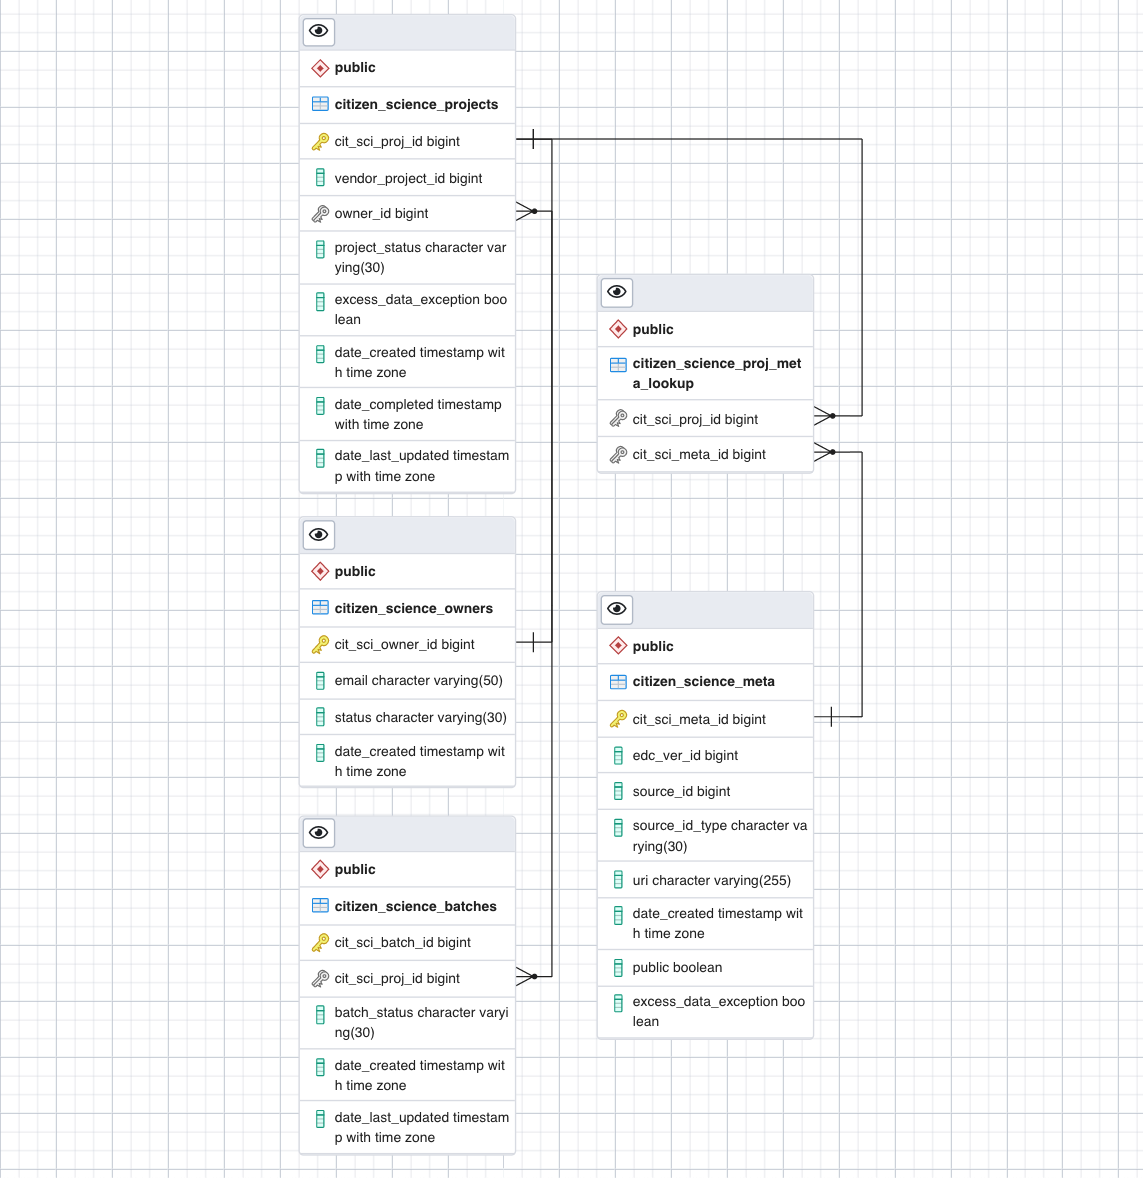
\includegraphics[width=3.12500in]{jira_imgs/2420.png}

}
\hdashrule[0.5ex]{\textwidth}{1pt}{3mm}
  Expected Result \\
{\footnotesize
The integrity of the citizen science tables can be verified.

}

\begin{tabular}{p{2cm}}
\toprule
Step 3  \\ \hline
\end{tabular}
 Description \\
{\footnotesize
Open up the following diagram which shows the structure of the Astro
Objects tables in the EDC to observe how the data is structured in order
to maintain scale precision and data integrity between the IDF and the
EDC.

}
\hdashrule[0.5ex]{\textwidth}{1pt}{3mm}
  Test Data \\
 {\footnotesize
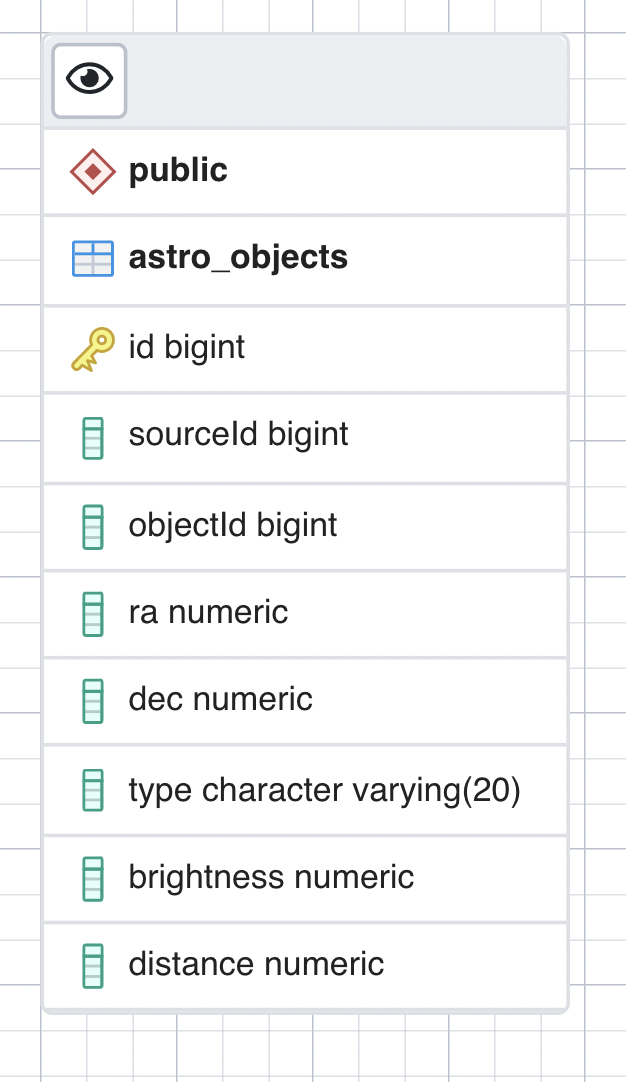
\includegraphics[width=3.12500in]{jira_imgs/2421.png}

}
\hdashrule[0.5ex]{\textwidth}{1pt}{3mm}
  Expected Result \\
{\footnotesize
The integrity of the Astro Objects table can be verified

}

\paragraph{ LVV-T2616 - Verify the Database Cluster in the EDC }\mbox{}\\

Version \textbf{1}.
Open  \href{https://jira.lsstcorp.org/secure/Tests.jspa#/testCase/LVV-T2616}{\textit{ LVV-T2616 } }
test case in Jira.

Verify the Database Cluster in the EDC

\textbf{ Preconditions}:\\


Final comment:\\\href{https://docushare.lsstcorp.org/docushare/dsweb/Get/Document-40975/EPO\%20-\%20Google\%20Cloud\%20-\%20Req\%20Ver.mp4}{\textbf{EPO
- Google Cloud - Req Ver}}\\
\textbf{Timemark:} 16:15


Detailed steps :

\begin{tabular}{p{2cm}}
\toprule
Step 1  \\ \hline
\end{tabular}
 Description \\
{\footnotesize
Open a web browser on a device connected to the internet, the type of
browser does not matter.

}
\hdashrule[0.5ex]{\textwidth}{1pt}{3mm}
  Expected Result \\
{\footnotesize
A web browser opens on the user's internet connected device

}

\begin{tabular}{p{2cm}}
\toprule
Step 2  \\ \hline
\end{tabular}
 Description \\
{\footnotesize
Type the following URL in the browser nav bar:

\begin{itemize}
\tightlist
\item
  https://github.com/lsst-epo/edc-deploy/blob/master/environment/deployments/epo/database/rubin/variables.tf\#L157-L180
\end{itemize}

}
\hdashrule[0.5ex]{\textwidth}{1pt}{3mm}
  Expected Result \\
{\footnotesize
The Github repository Terraform code previewer opens up in the browser.

}

\begin{tabular}{p{2cm}}
\toprule
Step 3  \\ \hline
\end{tabular}
 Description \\
{\footnotesize
Take note of the highlighted sections which defines that a read-only
replica will be created.

}
\hdashrule[0.5ex]{\textwidth}{1pt}{3mm}
  Expected Result \\
{\footnotesize
The Terraform code responsible for creating a read-only replicate is
visible in the browser.

}

\paragraph{ LVV-T2612 - Verify Object Store in EDC }\mbox{}\\

Version \textbf{1}.
Open  \href{https://jira.lsstcorp.org/secure/Tests.jspa#/testCase/LVV-T2612}{\textit{ LVV-T2612 } }
test case in Jira.

Verify that the EDC has the ability to store objects in an object store

\textbf{ Preconditions}:\\


Final comment:\\\href{https://docushare.lsstcorp.org/docushare/dsweb/Get/Document-40975/EPO\%20-\%20Google\%20Cloud\%20-\%20Req\%20Ver.mp4}{\textbf{EPO
- Google Cloud - Req Ver}}\\
\textbf{Timemark:} 4:55


Detailed steps :

\begin{tabular}{p{2cm}}
\toprule
Step 1  \\ \hline
\end{tabular}
 Description \\
{\footnotesize
Open a web browser on a device connected to the internet

}
\hdashrule[0.5ex]{\textwidth}{1pt}{3mm}
  Expected Result \\
{\footnotesize
A web browser opens on the internet-connected device

}

\begin{tabular}{p{2cm}}
\toprule
Step 2  \\ \hline
\end{tabular}
 Description \\
{\footnotesize
Type the following URL in the browser nav/URL bar:

\begin{itemize}
\tightlist
\item
  \url{https://console.cloud.google.com/}
\end{itemize}

}
\hdashrule[0.5ex]{\textwidth}{1pt}{3mm}
  Expected Result \\
{\footnotesize
\url{https://console.cloud.google.com/} loads in the browser.

}

\begin{tabular}{p{2cm}}
\toprule
Step 3  \\ \hline
\end{tabular}
 Description \\
{\footnotesize
Enter your @lsst.cloud email address in the ``Email or phone'' input
field

}
\hdashrule[0.5ex]{\textwidth}{1pt}{3mm}
  Expected Result \\
{\footnotesize
The email address of the user logging into the Google Cloud console
appears in the input field.

}

\begin{tabular}{p{2cm}}
\toprule
Step 4  \\ \hline
\end{tabular}
 Description \\
{\footnotesize
Click the ``Next'' button

}
\hdashrule[0.5ex]{\textwidth}{1pt}{3mm}
  Expected Result \\
{\footnotesize
The next page starts to load.

}

\begin{tabular}{p{2cm}}
\toprule
Step 5  \\ \hline
\end{tabular}
 Description \\
{\footnotesize
Enter your password in the password field.

}
\hdashrule[0.5ex]{\textwidth}{1pt}{3mm}
  Expected Result \\
{\footnotesize
The obfuscated password appears in the password field.

}

\begin{tabular}{p{2cm}}
\toprule
Step 6  \\ \hline
\end{tabular}
 Description \\
{\footnotesize
If prompted that 2-factor authentication is required to log in, click
``next'' and verify text on the page states that you will receive a text
message with a verification code.

}
\hdashrule[0.5ex]{\textwidth}{1pt}{3mm}
  Expected Result \\
{\footnotesize
2FA process is stated clearly on the screen.

}

\begin{tabular}{p{2cm}}
\toprule
Step 7  \\ \hline
\end{tabular}
 Description \\
{\footnotesize
Check your mobile device for a text message or Google message indicating
the verification code.

}
\hdashrule[0.5ex]{\textwidth}{1pt}{3mm}
  Expected Result \\
{\footnotesize
The verification code has been found on the user's device.

}

\begin{tabular}{p{2cm}}
\toprule
Step 8  \\ \hline
\end{tabular}
 Description \\
{\footnotesize
Enter the verification code from your mobile device into the input field
as indicated on the 2FA page in the browser and click next.

}
\hdashrule[0.5ex]{\textwidth}{1pt}{3mm}
  Expected Result \\
{\footnotesize
The Google form accepts the 2FA verification code.

}

\begin{tabular}{p{2cm}}
\toprule
Step 9  \\ \hline
\end{tabular}
 Description \\
{\footnotesize
The browser will then load the Google Cloud Platform dashboard, in the
``Select from'' dropdown in the modal that appears, select
``LSST.CLOUD''

}
\hdashrule[0.5ex]{\textwidth}{1pt}{3mm}
  Expected Result \\
{\footnotesize
A list of project will propagate once ``LSST.CLOUD'' is selected.

}

\begin{tabular}{p{2cm}}
\toprule
Step 10  \\ \hline
\end{tabular}
 Description \\
{\footnotesize
In the ``Search projects and folders'' search bar, type ``edc''

}
\hdashrule[0.5ex]{\textwidth}{1pt}{3mm}
  Expected Result \\
{\footnotesize
A list of projects prefixed with the letters ``edc'' will appear.

}

\begin{tabular}{p{2cm}}
\toprule
Step 11  \\ \hline
\end{tabular}
 Description \\
{\footnotesize
Click on ``edc-prod'' project

}
\hdashrule[0.5ex]{\textwidth}{1pt}{3mm}
  Expected Result \\
{\footnotesize
The ``edc-prod'' project will load.

}

\begin{tabular}{p{2cm}}
\toprule
Step 12  \\ \hline
\end{tabular}
 Description \\
{\footnotesize
Click on the three horizontal ``hamburger'' menu in the top left of the
page to expand the left-handed sidemenu

}
\hdashrule[0.5ex]{\textwidth}{1pt}{3mm}
  Expected Result \\
{\footnotesize
The left-handed side menu appears~

}

\begin{tabular}{p{2cm}}
\toprule
Step 13  \\ \hline
\end{tabular}
 Description \\
{\footnotesize
Scroll down to the ``Storage'' section of the side menu and click on
``Cloud Storage''

}
\hdashrule[0.5ex]{\textwidth}{1pt}{3mm}
  Expected Result \\
{\footnotesize
The Cloud Storage page loads in the main content area of the website,
with the title ``Bucket Browser'' appearing on the page

}

\begin{tabular}{p{2cm}}
\toprule
Step 14  \\ \hline
\end{tabular}
 Description \\
{\footnotesize
Note the various buckets, click on one of them (click on the ``Name'' of
the bucket)

}
\hdashrule[0.5ex]{\textwidth}{1pt}{3mm}
  Expected Result \\
{\footnotesize
The contents of that bucket loads in the table

}

\begin{tabular}{p{2cm}}
\toprule
Step 15  \\ \hline
\end{tabular}
 Description \\
{\footnotesize
\begin{longtable}[]{@{}l@{}}
\toprule
Note the files contained and the details of the bucket, this is the
object store and how it stores data\tabularnewline
\tabularnewline
\bottomrule
\end{longtable}

}
\hdashrule[0.5ex]{\textwidth}{1pt}{3mm}
  Expected Result \\
{\footnotesize
The objects in the object store are visible and can be observed

}

\paragraph{ LVV-T2614 - Verify Object Store Capacity in the EDC }\mbox{}\\

Version \textbf{1}.
Open  \href{https://jira.lsstcorp.org/secure/Tests.jspa#/testCase/LVV-T2614}{\textit{ LVV-T2614 } }
test case in Jira.

To Verify Object Store Capacity in the EDC

\textbf{ Preconditions}:\\


Final comment:\\\href{https://docushare.lsstcorp.org/docushare/dsweb/Get/Document-40975/EPO\%20-\%20Google\%20Cloud\%20-\%20Req\%20Ver.mp4}{\textbf{EPO
- Google Cloud - Req Ver}}\\
\textbf{Timemark:} 13:40


Detailed steps :

\begin{tabular}{p{2cm}}
\toprule
Step 1  \\ \hline
\end{tabular}
 Description \\
{\footnotesize
Open a web browser on a device connected to the internet. The type of
browser shouldn't matter.

}
\hdashrule[0.5ex]{\textwidth}{1pt}{3mm}
  Expected Result \\
{\footnotesize
A web browser opens up on the internet-connected device.

}

\begin{tabular}{p{2cm}}
\toprule
Step 2  \\ \hline
\end{tabular}
 Description \\
{\footnotesize
{Copy the following URL and paste it in the browser nav bar:}

\begin{itemize}
\tightlist
\item
  \href{https://cloud.google.com/blog/products/storage-data-transfer/how-does-your-cloud-storage-grow-with-a-scalable-plan-and-a-price-drop\#:~:text=You\%20can\%20use\%20Transfer\%20Appliance\%20to\%20get\%20petabytes\%20into\%20Cloud\%20Storage}{{https://cloud.google.com/blog/products/storage-data-transfer/how-does-your-cloud-storage-grow-with-a-scalable-plan-and-a-price-drop\#:\textasciitilde{}:text=You\%20can\%20use\%20Transfer\%20Appliance\%20to\%20get\%20petabytes\%20into\%20Cloud\%20Storage}}
\end{itemize}

}
\hdashrule[0.5ex]{\textwidth}{1pt}{3mm}
  Expected Result \\
{\footnotesize
The Google Cloud documentation page loads in the browser

}

\begin{tabular}{p{2cm}}
\toprule
Step 3  \\ \hline
\end{tabular}
 Description \\
{\footnotesize
Read the full article or, for brevity, scroll down to the third
paragraph and note the text ``You can use Transfer Appliance to get
petabytes into Cloud Storage quickly\ldots{}''

}
\hdashrule[0.5ex]{\textwidth}{1pt}{3mm}
  Expected Result \\
{\footnotesize
Observe how the documentation states that it is possible to start
petabytes of data in the Object Store.

}

\paragraph{ LVV-T2613 - Verify Object Store Quantity in EDC }\mbox{}\\

Version \textbf{1}.
Open  \href{https://jira.lsstcorp.org/secure/Tests.jspa#/testCase/LVV-T2613}{\textit{ LVV-T2613 } }
test case in Jira.

Verify Object Store Quantity in EDC

\textbf{ Preconditions}:\\


Final comment:\\\href{https://docushare.lsstcorp.org/docushare/dsweb/Get/Document-40975/EPO\%20-\%20Google\%20Cloud\%20-\%20Req\%20Ver.mp4}{\textbf{EPO
- Google Cloud - Req Ver}}\\
\textbf{Timemark:} 6:00


Detailed steps :

\begin{tabular}{p{2cm}}
\toprule
Step 1  \\ \hline
\end{tabular}
 Description \\
{\footnotesize
Open a web browser on a device connected to the internet

}
\hdashrule[0.5ex]{\textwidth}{1pt}{3mm}
  Expected Result \\
{\footnotesize
A web browser opens on the internet-connected device

}

\begin{tabular}{p{2cm}}
\toprule
Step 2  \\ \hline
\end{tabular}
 Description \\
{\footnotesize
Type the following URL in the browser nav/URL bar:

\begin{itemize}
\tightlist
\item
  \url{https://console.cloud.google.com/}
\end{itemize}

}
\hdashrule[0.5ex]{\textwidth}{1pt}{3mm}
  Expected Result \\
{\footnotesize
\url{https://console.cloud.google.com/} loads in the browser.

}

\begin{tabular}{p{2cm}}
\toprule
Step 3  \\ \hline
\end{tabular}
 Description \\
{\footnotesize
Enter your @lsst.cloud email address in the ``Email or phone'' input
field

}
\hdashrule[0.5ex]{\textwidth}{1pt}{3mm}
  Expected Result \\
{\footnotesize
The email address of the user logging into the Google Cloud console
appears in the input field.

}

\begin{tabular}{p{2cm}}
\toprule
Step 4  \\ \hline
\end{tabular}
 Description \\
{\footnotesize
Click the ``Next'' button

}
\hdashrule[0.5ex]{\textwidth}{1pt}{3mm}
  Expected Result \\
{\footnotesize
The next page starts to load.

}

\begin{tabular}{p{2cm}}
\toprule
Step 5  \\ \hline
\end{tabular}
 Description \\
{\footnotesize
Enter your password in the password field.

}
\hdashrule[0.5ex]{\textwidth}{1pt}{3mm}
  Expected Result \\
{\footnotesize
The obfuscated password appears in the password field.

}

\begin{tabular}{p{2cm}}
\toprule
Step 6  \\ \hline
\end{tabular}
 Description \\
{\footnotesize
If prompted that 2-factor authentication is required to log in, click
``next'' and verify text on the page states that you will receive a text
message with a verification code.

}
\hdashrule[0.5ex]{\textwidth}{1pt}{3mm}
  Expected Result \\
{\footnotesize
2FA process is stated clearly on the screen.

}

\begin{tabular}{p{2cm}}
\toprule
Step 7  \\ \hline
\end{tabular}
 Description \\
{\footnotesize
Check your mobile device for a text message or Google message indicating
the verification code.

}
\hdashrule[0.5ex]{\textwidth}{1pt}{3mm}
  Expected Result \\
{\footnotesize
The verification code has been found on the user's device.

}

\begin{tabular}{p{2cm}}
\toprule
Step 8  \\ \hline
\end{tabular}
 Description \\
{\footnotesize
Enter the verification code from your mobile device into the input field
as indicated on the 2FA page in the browser and click next.

}
\hdashrule[0.5ex]{\textwidth}{1pt}{3mm}
  Expected Result \\
{\footnotesize
The Google form accepts the 2FA verification code.

}

\begin{tabular}{p{2cm}}
\toprule
Step 9  \\ \hline
\end{tabular}
 Description \\
{\footnotesize
The browser will then load the Google Cloud Platform dashboard, in the
``Select from'' dropdown in the modal that appears, select
``LSST.CLOUD''

}
\hdashrule[0.5ex]{\textwidth}{1pt}{3mm}
  Expected Result \\
{\footnotesize
A list of project will propagate once ``LSST.CLOUD'' is selected.

}

\begin{tabular}{p{2cm}}
\toprule
Step 10  \\ \hline
\end{tabular}
 Description \\
{\footnotesize
In the ``Search projects and folders'' search bar, type ``edc''

}
\hdashrule[0.5ex]{\textwidth}{1pt}{3mm}
  Expected Result \\
{\footnotesize
A list of projects prefixed with the letters ``edc'' will appear.

}

\begin{tabular}{p{2cm}}
\toprule
Step 11  \\ \hline
\end{tabular}
 Description \\
{\footnotesize
Click on ``edc-prod'' project

}
\hdashrule[0.5ex]{\textwidth}{1pt}{3mm}
  Expected Result \\
{\footnotesize
The ``edc-prod'' project will load.

}

\begin{tabular}{p{2cm}}
\toprule
Step 12  \\ \hline
\end{tabular}
 Description \\
{\footnotesize
Click on the three horizontal ``hamburger'' menu in the top left of the
page to expand the left-handed side menu

}
\hdashrule[0.5ex]{\textwidth}{1pt}{3mm}
  Expected Result \\
{\footnotesize
The left-handed side menu appears

}

\begin{tabular}{p{2cm}}
\toprule
Step 13  \\ \hline
\end{tabular}
 Description \\
{\footnotesize
Scroll down to the ``Operations'' section of the side menu and click on
``Monitoring''

}
\hdashrule[0.5ex]{\textwidth}{1pt}{3mm}
  Expected Result \\
{\footnotesize
The Monitoring page loads in the main content area of the website

}

\begin{tabular}{p{2cm}}
\toprule
Step 14  \\ \hline
\end{tabular}
 Description \\
{\footnotesize
On the left-side of the page in the side menu under the ``Monitoring''
header, click ``Metrics explorer'' menu item

}
\hdashrule[0.5ex]{\textwidth}{1pt}{3mm}
  Expected Result \\
{\footnotesize
The Metrics Explorer loads~

}

\begin{tabular}{p{2cm}}
\toprule
Step 15  \\ \hline
\end{tabular}
 Description \\
{\footnotesize
On the ``Metrics explorer'' page that loads, click the ``SELECT A
METRIC'' dropdown

}
\hdashrule[0.5ex]{\textwidth}{1pt}{3mm}
  Expected Result \\
{\footnotesize
The dropdown appears with options to select

}

\begin{tabular}{p{2cm}}
\toprule
Step 16  \\ \hline
\end{tabular}
 Description \\
{\footnotesize
Scroll down in the dropdown to ``GCS Bucket'' and hover over this option

}
\hdashrule[0.5ex]{\textwidth}{1pt}{3mm}
  Expected Result \\
{\footnotesize
A new dropdown menu will appear to the right

}

\begin{tabular}{p{2cm}}
\toprule
Step 17  \\ \hline
\end{tabular}
 Description \\
{\footnotesize
In the new dropdown menu, click ``Storage''

}
\hdashrule[0.5ex]{\textwidth}{1pt}{3mm}
  Expected Result \\
{\footnotesize
A new dropdown menu will appear to the right again

}

\begin{tabular}{p{2cm}}
\toprule
Step 18  \\ \hline
\end{tabular}
 Description \\
{\footnotesize
In the new dropdown menu, click ``Object count''

}
\hdashrule[0.5ex]{\textwidth}{1pt}{3mm}
  Expected Result \\
{\footnotesize
The ``Object count'' option will be selected

}

\begin{tabular}{p{2cm}}
\toprule
Step 19  \\ \hline
\end{tabular}
 Description \\
{\footnotesize
Click the ``Apply'' button~

}
\hdashrule[0.5ex]{\textwidth}{1pt}{3mm}
  Expected Result \\
{\footnotesize
The dropdown closes

}

\begin{tabular}{p{2cm}}
\toprule
Step 20  \\ \hline
\end{tabular}
 Description \\
{\footnotesize
In the ``How do you want to view that data'' section that appears on the
page, click the ``Aggregator'' dropdown

}
\hdashrule[0.5ex]{\textwidth}{1pt}{3mm}
  Expected Result \\
{\footnotesize
A new dropdown appears

}

\begin{tabular}{p{2cm}}
\toprule
Step 21  \\ \hline
\end{tabular}
 Description \\
{\footnotesize
Select ``sum'' in the dropdown

}
\hdashrule[0.5ex]{\textwidth}{1pt}{3mm}
  Expected Result \\
{\footnotesize
The ``sum'' option is selected

}

\begin{tabular}{p{2cm}}
\toprule
Step 22  \\ \hline
\end{tabular}
 Description \\
{\footnotesize
Note the metric ``object\_count'' to the right of the dropdown, the
``Value'' column represents how many objects (files) are within the
object store, note that it is over 100,000 in value

}
\hdashrule[0.5ex]{\textwidth}{1pt}{3mm}
  Expected Result \\
{\footnotesize
The object count capacity is observed

}

\paragraph{ LVV-T2621 - Verify that image data can be preserved in the EDC object store }\mbox{}\\

Version \textbf{1}.
Open  \href{https://jira.lsstcorp.org/secure/Tests.jspa#/testCase/LVV-T2621}{\textit{ LVV-T2621 } }
test case in Jira.

The objective of this test case is to verify that image data can be
preserved in the EDC object store.

\textbf{ Preconditions}:\\


Final comment:\\\href{https://docushare.lsstcorp.org/docushare/dsweb/Get/Document-40975/EPO\%20-\%20Google\%20Cloud\%20-\%20Req\%20Ver.mp4}{\textbf{EPO
- Google Cloud - Req Ver}}\\
\textbf{Timemark:} 7:30\\
\&\\
\textbf{Timemark:} 15:30


Detailed steps :

\begin{tabular}{p{2cm}}
\toprule
Step 1  \\ \hline
\end{tabular}
 Description \\
{\footnotesize
Open a web browser on a device connected to the internet

}
\hdashrule[0.5ex]{\textwidth}{1pt}{3mm}
  Expected Result \\
{\footnotesize
A web browser opens on the internet-connected device

}

\begin{tabular}{p{2cm}}
\toprule
Step 2  \\ \hline
\end{tabular}
 Description \\
{\footnotesize
Type the following URL in the browser nav/URL bar:

\begin{itemize}
\tightlist
\item
  \url{https://console.cloud.google.com/}
\end{itemize}

}
\hdashrule[0.5ex]{\textwidth}{1pt}{3mm}
  Expected Result \\
{\footnotesize
\url{https://console.cloud.google.com/} loads in the browser.

}

\begin{tabular}{p{2cm}}
\toprule
Step 3  \\ \hline
\end{tabular}
 Description \\
{\footnotesize
Enter your @lsst.cloud email address in the ``Email or phone'' input
field

}
\hdashrule[0.5ex]{\textwidth}{1pt}{3mm}
  Expected Result \\
{\footnotesize
The email address of the user logging into the Google Cloud console
appears in the input field.

}

\begin{tabular}{p{2cm}}
\toprule
Step 4  \\ \hline
\end{tabular}
 Description \\
{\footnotesize
Click the ``Next'' button

}
\hdashrule[0.5ex]{\textwidth}{1pt}{3mm}
  Expected Result \\
{\footnotesize
The next page starts to load.

}

\begin{tabular}{p{2cm}}
\toprule
Step 5  \\ \hline
\end{tabular}
 Description \\
{\footnotesize
Enter your password in the password field.

}
\hdashrule[0.5ex]{\textwidth}{1pt}{3mm}
  Expected Result \\
{\footnotesize
The obfuscated password appears in the password field.

}

\begin{tabular}{p{2cm}}
\toprule
Step 6  \\ \hline
\end{tabular}
 Description \\
{\footnotesize
If prompted that 2-factor authentication is required to log in, click
``next'' and verify text on the page states that you will receive a text
message with a verification code.

}
\hdashrule[0.5ex]{\textwidth}{1pt}{3mm}
  Expected Result \\
{\footnotesize
2FA process is stated clearly on the screen.

}

\begin{tabular}{p{2cm}}
\toprule
Step 7  \\ \hline
\end{tabular}
 Description \\
{\footnotesize
Check your mobile device for a text message or Google message indicating
the verification code.

}
\hdashrule[0.5ex]{\textwidth}{1pt}{3mm}
  Expected Result \\
{\footnotesize
The verification code has been found on the user's device.

}

\begin{tabular}{p{2cm}}
\toprule
Step 8  \\ \hline
\end{tabular}
 Description \\
{\footnotesize
Enter the verification code from your mobile device into the input field
as indicated on the 2FA page in the browser and click next.

}
\hdashrule[0.5ex]{\textwidth}{1pt}{3mm}
  Expected Result \\
{\footnotesize
The Google form accepts the 2FA verification code.

}

\begin{tabular}{p{2cm}}
\toprule
Step 9  \\ \hline
\end{tabular}
 Description \\
{\footnotesize
The browser will then load the Google Cloud Platform dashboard, in the
``Select from'' dropdown in the modal that appears, select
``LSST.CLOUD''

}
\hdashrule[0.5ex]{\textwidth}{1pt}{3mm}
  Expected Result \\
{\footnotesize
A list of project will propagate once ``LSST.CLOUD'' is selected.

}

\begin{tabular}{p{2cm}}
\toprule
Step 10  \\ \hline
\end{tabular}
 Description \\
{\footnotesize
In the ``Search projects and folders'' search bar, type ``edc''

}
\hdashrule[0.5ex]{\textwidth}{1pt}{3mm}
  Expected Result \\
{\footnotesize
A list of projects prefixed with the letters ``edc'' will appear.

}

\begin{tabular}{p{2cm}}
\toprule
Step 11  \\ \hline
\end{tabular}
 Description \\
{\footnotesize
Click on ``edc-prod'' project

}
\hdashrule[0.5ex]{\textwidth}{1pt}{3mm}
  Expected Result \\
{\footnotesize
The ``edc-prod'' project will load.

}

\begin{tabular}{p{2cm}}
\toprule
Step 12  \\ \hline
\end{tabular}
 Description \\
{\footnotesize
Click on the three horizontal ``hamburger'' menu in the top left of the
page to expand the left-handed side menu

}
\hdashrule[0.5ex]{\textwidth}{1pt}{3mm}
  Expected Result \\
{\footnotesize
The left-handed side menu opens up

}

\begin{tabular}{p{2cm}}
\toprule
Step 13  \\ \hline
\end{tabular}
 Description \\
{\footnotesize
In the left-handed side menu, scroll down to ``Storage'' and click on
``Cloud Storage''

}
\hdashrule[0.5ex]{\textwidth}{1pt}{3mm}
  Expected Result \\
{\footnotesize
The Cloud Storage page loads in the main content area of the website

}

\begin{tabular}{p{2cm}}
\toprule
Step 14  \\ \hline
\end{tabular}
 Description \\
{\footnotesize
Click on the ``alerts-stream-data'' bucket in the ``Browser'' table and
the ``Bucket details'' page will open for that bucket

}
\hdashrule[0.5ex]{\textwidth}{1pt}{3mm}
  Expected Result \\
{\footnotesize
The ``alerts-payloads'' bucket details loads

}

\begin{tabular}{p{2cm}}
\toprule
Step 15  \\ \hline
\end{tabular}
 Description \\
{\footnotesize
In the ``Name'' column, click an alert image and the ``Object details''
page will open for that file

}
\hdashrule[0.5ex]{\textwidth}{1pt}{3mm}
  Expected Result \\
{\footnotesize
The object details page loads

}

\begin{tabular}{p{2cm}}
\toprule
Step 16  \\ \hline
\end{tabular}
 Description \\
{\footnotesize
Click the ``DOWNLOAD'' link

}
\hdashrule[0.5ex]{\textwidth}{1pt}{3mm}
  Expected Result \\
{\footnotesize
The image downloads

}

\begin{tabular}{p{2cm}}
\toprule
Step 17  \\ \hline
\end{tabular}
 Description \\
{\footnotesize
Click on the browser file download icon that appears at the bottom of
the browser once the download finishes

}
\hdashrule[0.5ex]{\textwidth}{1pt}{3mm}
  Expected Result \\
{\footnotesize
The image loads and a preview for the image is shown on the screen

}

\paragraph{ LVV-T2619 - Verify that textual data from the alert broker can be stored in a
relational, tabular database }\mbox{}\\

Version \textbf{1}.
Open  \href{https://jira.lsstcorp.org/secure/Tests.jspa#/testCase/LVV-T2619}{\textit{ LVV-T2619 } }
test case in Jira.

The objective of this test case is to verify that textual data from the
alert broker can be stored in a relational, tabular database.

\textbf{ Preconditions}:\\


Final comment:\\\href{https://docushare.lsstcorp.org/docushare/dsweb/Get/Document-40975/EPO\%20-\%20Google\%20Cloud\%20-\%20Req\%20Ver.mp4}{\textbf{EPO
- Google Cloud - Req Ver}}\\
\textbf{Timemark:} 7:30\\
\&\\
\textbf{Timemark:} 15:30


Detailed steps :

\begin{tabular}{p{2cm}}
\toprule
Step 1  \\ \hline
\end{tabular}
 Description \\
{\footnotesize
Open the Terminal app on an internet connected device Macbook~

}
\hdashrule[0.5ex]{\textwidth}{1pt}{3mm}
  Expected Result \\
{\footnotesize
The Terminal app opens on the internet connected device.

}

\begin{tabular}{p{2cm}}
\toprule
Step 2  \\ \hline
\end{tabular}
 Description \\
{\footnotesize
Enter the following command and then hit enter:

\begin{itemize}
\tightlist
\item
  cd \textasciitilde{}
\end{itemize}

}
\hdashrule[0.5ex]{\textwidth}{1pt}{3mm}
  Expected Result \\
{\footnotesize
The Terminal app navigates to the user's home directory.

}

\begin{tabular}{p{2cm}}
\toprule
Step 3  \\ \hline
\end{tabular}
 Description \\
{\footnotesize
Enter the following command and then hit enter:

\begin{itemize}
\tightlist
\item
  gcloud sql export sql --project edc-prod-eef0 astro\_artifacts
  \href{gs\%3A//skyviewer/skyviewer-export.sql}{gs://astro-artifacts-dumps/alerts-db-export.sql}
  --database=astro\_artifacts
\end{itemize}

}
\hdashrule[0.5ex]{\textwidth}{1pt}{3mm}
  Expected Result \\
{\footnotesize
The output in the terminal indicates that a SQL dump file was created in
a prod Google Cloud bucket named ``astro-artifacts-dumps''

}

\begin{tabular}{p{2cm}}
\toprule
Step 4  \\ \hline
\end{tabular}
 Description \\
{\footnotesize
Enter the following command and then hit enter:

\begin{itemize}
\tightlist
\item
  gsutil
  cp~\href{gs\%3A//skyviewer/skyviewer-export.sql}{gs://astro-artifacts-dumps/alerts-db-export.sql}
  \textasciitilde{}/alerts-db-export.sql
\end{itemize}

}
\hdashrule[0.5ex]{\textwidth}{1pt}{3mm}
  Expected Result \\
{\footnotesize
The SQL dump file is downloaded to the user's computer in the home
directory with the name ``alerts-db-export.sql''

}

\begin{tabular}{p{2cm}}
\toprule
Step 5  \\ \hline
\end{tabular}
 Description \\
{\footnotesize
Open up a text editing/viewing application

}
\hdashrule[0.5ex]{\textwidth}{1pt}{3mm}
  Expected Result \\
{\footnotesize
A text editing/viewing app opens up

}

\begin{tabular}{p{2cm}}
\toprule
Step 6  \\ \hline
\end{tabular}
 Description \\
{\footnotesize
Select the text editing/viewing application's option to open a file

}
\hdashrule[0.5ex]{\textwidth}{1pt}{3mm}
  Expected Result \\
{\footnotesize
A window appears to select a file to open

}

\begin{tabular}{p{2cm}}
\toprule
Step 7  \\ \hline
\end{tabular}
 Description \\
{\footnotesize
Select the file ``alerts-db-export.sql'' in the user's home directory to
open it up for viewing

}
\hdashrule[0.5ex]{\textwidth}{1pt}{3mm}
  Expected Result \\
{\footnotesize
The ``alerts-db-exporter.sql'' file opens up in the text editing/viewing
app.

}

\begin{tabular}{p{2cm}}
\toprule
Step 8  \\ \hline
\end{tabular}
 Description \\
{\footnotesize
With the text editing/viewing application in focus, hold the Control key
and press the `F' key to pull up the ``find in document'' window

}
\hdashrule[0.5ex]{\textwidth}{1pt}{3mm}
  Expected Result \\
{\footnotesize
The search window appears in the text editing/viewing application.

}

\begin{tabular}{p{2cm}}
\toprule
Step 9  \\ \hline
\end{tabular}
 Description \\
{\footnotesize
In the ``search for'' box, type ``create table alerts'' and click
``Search'' or ``Find'' to have the file autoscroll to the part of the
SQL script that defines the table that holds the alert data

}
\hdashrule[0.5ex]{\textwidth}{1pt}{3mm}
  Expected Result \\
{\footnotesize
The part of the SQL dump file that defines the creation of the alerts
table is auto-scrolled to in the text editing/viewing app.

}

\begin{tabular}{p{2cm}}
\toprule
Step 10  \\ \hline
\end{tabular}
 Description \\
{\footnotesize
Note the columns defined to hold the alerts data

}
\hdashrule[0.5ex]{\textwidth}{1pt}{3mm}
  Expected Result \\
{\footnotesize
The column definitions can be observed

}

\begin{tabular}{p{2cm}}
\toprule
Step 11  \\ \hline
\end{tabular}
 Description \\
{\footnotesize
In the ``search for'' box of the search window, replace the text
``create table alerts'' with ``Data for Name: alerts'' and hit
``Search''

}
\hdashrule[0.5ex]{\textwidth}{1pt}{3mm}
  Expected Result \\
{\footnotesize
The text editing/viewing app auto-scrolls to the section of the SQL dump
file that shows the tabular alerts data.

}

\begin{tabular}{p{2cm}}
\toprule
Step 12  \\ \hline
\end{tabular}
 Description \\
{\footnotesize
Note the alert data in text format

}
\hdashrule[0.5ex]{\textwidth}{1pt}{3mm}
  Expected Result \\
{\footnotesize
The alert data in tabular text format is observed.

}

\paragraph{ LVV-T2662 - Verify that the App Engine API projects can handle 80 concurrent
requests }\mbox{}\\

Version \textbf{1}.
Open  \href{https://jira.lsstcorp.org/secure/Tests.jspa#/testCase/LVV-T2662}{\textit{ LVV-T2662 } }
test case in Jira.

Verify that the App Engine API projects can handle 80 concurrent
requests

\textbf{ Preconditions}:\\


Final comment:\\\href{https://docushare.lsstcorp.org/docushare/dsweb/Get/Document-40975/EPO\%20-\%20Google\%20Cloud\%20-\%20Req\%20Ver.mp4}{\textbf{EPO
- Google Cloud - Req Ver}}\\
\textbf{Timemark:} 10:00\\
\textbf{Also:}\\
\href{https://docushare.lsstcorp.org/docushare/dsweb/Get/Document-43308/Rubin\%20EPO\%20Requirements\%20Validation\%20.pdf}{\textbf{Rubin
EPO Requirements Validation .pdf}~}


Detailed steps :

\begin{tabular}{p{2cm}}
\toprule
Step 1  \\ \hline
\end{tabular}
 Description \\
{\footnotesize
Open a web browser on a device connected to the internet

}
\hdashrule[0.5ex]{\textwidth}{1pt}{3mm}
  Expected Result \\
{\footnotesize
A web browser opens on the internet-connected device

}

\begin{tabular}{p{2cm}}
\toprule
Step 2  \\ \hline
\end{tabular}
 Description \\
{\footnotesize
Type the following URL in the browser nav/URL bar:

\begin{itemize}
\tightlist
\item
  \url{https://console.cloud.google.com/}
\end{itemize}

}
\hdashrule[0.5ex]{\textwidth}{1pt}{3mm}
  Expected Result \\
{\footnotesize
\url{https://console.cloud.google.com/} loads in the browser.

}

\begin{tabular}{p{2cm}}
\toprule
Step 3  \\ \hline
\end{tabular}
 Description \\
{\footnotesize
Enter your @lsst.cloud email address in the ``Email or phone'' input
field

}
\hdashrule[0.5ex]{\textwidth}{1pt}{3mm}
  Expected Result \\
{\footnotesize
The email address of the user logging into the Google Cloud console
appears in the input field.

}

\begin{tabular}{p{2cm}}
\toprule
Step 4  \\ \hline
\end{tabular}
 Description \\
{\footnotesize
Click the ``Next'' button

}
\hdashrule[0.5ex]{\textwidth}{1pt}{3mm}
  Expected Result \\
{\footnotesize
The next page starts to load.

}

\begin{tabular}{p{2cm}}
\toprule
Step 5  \\ \hline
\end{tabular}
 Description \\
{\footnotesize
Enter your password in the password field.

}
\hdashrule[0.5ex]{\textwidth}{1pt}{3mm}
  Expected Result \\
{\footnotesize
The obfuscated password appears in the password field.

}

\begin{tabular}{p{2cm}}
\toprule
Step 6  \\ \hline
\end{tabular}
 Description \\
{\footnotesize
If prompted that 2-factor authentication is required to log in, click
``next'' and verify text on the page states that you will receive a text
message with a verification code.

}
\hdashrule[0.5ex]{\textwidth}{1pt}{3mm}
  Expected Result \\
{\footnotesize
2FA process is stated clearly on the screen.

}

\begin{tabular}{p{2cm}}
\toprule
Step 7  \\ \hline
\end{tabular}
 Description \\
{\footnotesize
Check your mobile device for a text message or Google message indicating
the verification code.

}
\hdashrule[0.5ex]{\textwidth}{1pt}{3mm}
  Expected Result \\
{\footnotesize
The verification code has been found on the user's device.

}

\begin{tabular}{p{2cm}}
\toprule
Step 8  \\ \hline
\end{tabular}
 Description \\
{\footnotesize
Enter the verification code from your mobile device into the input field
as indicated on the 2FA page in the browser and click next.

}
\hdashrule[0.5ex]{\textwidth}{1pt}{3mm}
  Expected Result \\
{\footnotesize
The Google form accepts the 2FA verification code.

}

\begin{tabular}{p{2cm}}
\toprule
Step 9  \\ \hline
\end{tabular}
 Description \\
{\footnotesize
The browser will then load the Google Cloud Platform dashboard, in the
``Select from'' dropdown in the modal that appears, select
``LSST.CLOUD''

}
\hdashrule[0.5ex]{\textwidth}{1pt}{3mm}
  Expected Result \\
{\footnotesize
A list of project will propagate once ``LSST.CLOUD'' is selected.

}

\begin{tabular}{p{2cm}}
\toprule
Step 10  \\ \hline
\end{tabular}
 Description \\
{\footnotesize
In the ``Search projects and folders'' search bar, type ``edc''

}
\hdashrule[0.5ex]{\textwidth}{1pt}{3mm}
  Expected Result \\
{\footnotesize
A list of projects prefixed with the letters ``edc'' will appear.

}

\begin{tabular}{p{2cm}}
\toprule
Step 11  \\ \hline
\end{tabular}
 Description \\
{\footnotesize
Click on ``edc-prod'' project

}
\hdashrule[0.5ex]{\textwidth}{1pt}{3mm}
  Expected Result \\
{\footnotesize
The ``edc-prod'' project will load.

}

\begin{tabular}{p{2cm}}
\toprule
Step 12  \\ \hline
\end{tabular}
 Description \\
{\footnotesize
Open a web browser on a device connected to the internet

}
\hdashrule[0.5ex]{\textwidth}{1pt}{3mm}
  Expected Result \\
{\footnotesize
A web browser opens on the internet-connected device

}

\begin{tabular}{p{2cm}}
\toprule
Step 13  \\ \hline
\end{tabular}
 Description \\
{\footnotesize
Type the following URL in the browser nav/URL bar:

\begin{itemize}
\tightlist
\item
  \url{https://console.cloud.google.com/}
\end{itemize}

}
\hdashrule[0.5ex]{\textwidth}{1pt}{3mm}
  Expected Result \\
{\footnotesize
\url{https://console.cloud.google.com/} loads in the browser.

}

\begin{tabular}{p{2cm}}
\toprule
Step 14  \\ \hline
\end{tabular}
 Description \\
{\footnotesize
Enter your @lsst.cloud email address in the ``Email or phone'' input
field

}
\hdashrule[0.5ex]{\textwidth}{1pt}{3mm}
  Expected Result \\
{\footnotesize
The email address of the user logging into the Google Cloud console
appears in the input field.

}

\begin{tabular}{p{2cm}}
\toprule
Step 15  \\ \hline
\end{tabular}
 Description \\
{\footnotesize
Click the ``Next'' button

}
\hdashrule[0.5ex]{\textwidth}{1pt}{3mm}
  Expected Result \\
{\footnotesize
The next page starts to load.

}

\begin{tabular}{p{2cm}}
\toprule
Step 16  \\ \hline
\end{tabular}
 Description \\
{\footnotesize
Enter your password in the password field.

}
\hdashrule[0.5ex]{\textwidth}{1pt}{3mm}
  Expected Result \\
{\footnotesize
The obfuscated password appears in the password field.

}

\begin{tabular}{p{2cm}}
\toprule
Step 17  \\ \hline
\end{tabular}
 Description \\
{\footnotesize
If prompted that 2-factor authentication is required to log in, click
``next'' and verify text on the page states that you will receive a text
message with a verification code.

}
\hdashrule[0.5ex]{\textwidth}{1pt}{3mm}
  Expected Result \\
{\footnotesize
2FA process is stated clearly on the screen.

}

\begin{tabular}{p{2cm}}
\toprule
Step 18  \\ \hline
\end{tabular}
 Description \\
{\footnotesize
Check your mobile device for a text message or Google message indicating
the verification code.

}
\hdashrule[0.5ex]{\textwidth}{1pt}{3mm}
  Expected Result \\
{\footnotesize
The verification code has been found on the user's device.

}

\begin{tabular}{p{2cm}}
\toprule
Step 19  \\ \hline
\end{tabular}
 Description \\
{\footnotesize
Enter the verification code from your mobile device into the input field
as indicated on the 2FA page in the browser and click next.

}
\hdashrule[0.5ex]{\textwidth}{1pt}{3mm}
  Expected Result \\
{\footnotesize
The Google form accepts the 2FA verification code.

}

\begin{tabular}{p{2cm}}
\toprule
Step 20  \\ \hline
\end{tabular}
 Description \\
{\footnotesize
The browser will then load the Google Cloud Platform dashboard, in the
``Select from'' dropdown in the modal that appears, select
``LSST.CLOUD''

}
\hdashrule[0.5ex]{\textwidth}{1pt}{3mm}
  Expected Result \\
{\footnotesize
A list of project will propagate once ``LSST.CLOUD'' is selected.

}

\begin{tabular}{p{2cm}}
\toprule
Step 21  \\ \hline
\end{tabular}
 Description \\
{\footnotesize
In the ``Search projects and folders'' search bar, type ``edc''

}
\hdashrule[0.5ex]{\textwidth}{1pt}{3mm}
  Expected Result \\
{\footnotesize
A list of projects prefixed with the letters ``edc'' will appear.

}

\begin{tabular}{p{2cm}}
\toprule
Step 22  \\ \hline
\end{tabular}
 Description \\
{\footnotesize
Click on ``edc-prod'' project

}
\hdashrule[0.5ex]{\textwidth}{1pt}{3mm}
  Expected Result \\
{\footnotesize
The ``edc-prod'' project will load.

}

\begin{tabular}{p{2cm}}
\toprule
Step 23  \\ \hline
\end{tabular}
 Description \\
{\footnotesize
Click the hamburger menu with the three horizontal lines in the top left
of the page

}
\hdashrule[0.5ex]{\textwidth}{1pt}{3mm}
  Expected Result \\
{\footnotesize
The left-handed side menu expands from the left of the page

}

\begin{tabular}{p{2cm}}
\toprule
Step 24  \\ \hline
\end{tabular}
 Description \\
{\footnotesize
In the left-handed side menu, scroll down to the ``Security'' menu link
and click on it

}
\hdashrule[0.5ex]{\textwidth}{1pt}{3mm}
  Expected Result \\
{\footnotesize
The ``Security Command Center'' page opens up in the browser

}

\begin{tabular}{p{2cm}}
\toprule
Step 25  \\ \hline
\end{tabular}
 Description \\
{\footnotesize
On the left-hand side of the page, click on the ``Secret Manager'' link

}
\hdashrule[0.5ex]{\textwidth}{1pt}{3mm}
  Expected Result \\
{\footnotesize
The ``Secret Manager'' page loads in the browser

}

\begin{tabular}{p{2cm}}
\toprule
Step 26  \\ \hline
\end{tabular}
 Description \\
{\footnotesize
Click on any of the API projects, such as ``rubin-obs-api-appyaml''

}
\hdashrule[0.5ex]{\textwidth}{1pt}{3mm}
  Expected Result \\
{\footnotesize
The version information for the secret clicked on loads on the page

}

\begin{tabular}{p{2cm}}
\toprule
Step 27  \\ \hline
\end{tabular}
 Description \\
{\footnotesize
For the version with the highest number, which should also be at the top
of the versions table, click on the vertical three dots icon to the
right of the table

}
\hdashrule[0.5ex]{\textwidth}{1pt}{3mm}
  Expected Result \\
{\footnotesize
The options for that latest version appear on the screen

}

\begin{tabular}{p{2cm}}
\toprule
Step 28  \\ \hline
\end{tabular}
 Description \\
{\footnotesize
Click on the ``View Secret Value'' option

}
\hdashrule[0.5ex]{\textwidth}{1pt}{3mm}
  Expected Result \\
{\footnotesize
The ``Secret Value'' popup appears

}

\begin{tabular}{p{2cm}}
\toprule
Step 29  \\ \hline
\end{tabular}
 Description \\
{\footnotesize
Find the section of the secret that starts with ``automatic\_scaling:''

}
\hdashrule[0.5ex]{\textwidth}{1pt}{3mm}
  Expected Result \\
{\footnotesize
The ``automatic scaling'' section of the secret is visible on the screen

}

\begin{tabular}{p{2cm}}
\toprule
Step 30  \\ \hline
\end{tabular}
 Description \\
{\footnotesize
Note that the minimum instances are set to 4 and the maximum instances
are set to 5

}
\hdashrule[0.5ex]{\textwidth}{1pt}{3mm}
  Expected Result \\
{\footnotesize
The minimum and maximum number of instances are visible on the screen

}

\begin{tabular}{p{2cm}}
\toprule
Step 31  \\ \hline
\end{tabular}
 Description \\
{\footnotesize
Also in the same ``automatic\_scaling'' section, note that maximum
concurrent requests per instance is set to 80

}
\hdashrule[0.5ex]{\textwidth}{1pt}{3mm}
  Expected Result \\
{\footnotesize
The maximum number of concurrent requests is visible on the page

}

\paragraph{ LVV-T2618 - Verify the ability of the EDC to be configured for automatic scaling of
resources }\mbox{}\\

Version \textbf{1}.
Open  \href{https://jira.lsstcorp.org/secure/Tests.jspa#/testCase/LVV-T2618}{\textit{ LVV-T2618 } }
test case in Jira.

The objective of this test case is to verify the ability of the EDC to
be configured for automatic scaling of resources.

\textbf{ Preconditions}:\\


Final comment:\\\href{https://docushare.lsstcorp.org/docushare/dsweb/Get/Document-40975/EPO\%20-\%20Google\%20Cloud\%20-\%20Req\%20Ver.mp4}{\textbf{EPO
- Google Cloud - Req Ver}}\\
\textbf{Timemark:} 17:30


Detailed steps :

\begin{tabular}{p{2cm}}
\toprule
Step 1  \\ \hline
\end{tabular}
 Description \\
{\footnotesize
{Open a web browser on a device connected to the internet, the type of
browser does not matter.}

}
\hdashrule[0.5ex]{\textwidth}{1pt}{3mm}
  Expected Result \\
{\footnotesize
A web browser opens up on the internet-connected device.

}

\begin{tabular}{p{2cm}}
\toprule
Step 2  \\ \hline
\end{tabular}
 Description \\
{\footnotesize
{Type the following URL in the browser nav bar:}

\begin{itemize}
\tightlist
\item
  https://github.com/lsst-epo/edc-deploy/blob/b8559a569231fa6b59a9b2cdb115334d85ef00bb/environment/deployments/epo/env/int-database-rubin.tfvars\#L28
\end{itemize}

}
\hdashrule[0.5ex]{\textwidth}{1pt}{3mm}
  Expected Result \\
{\footnotesize
The Github page with the code preview for the PostgreSQL scaling option
of autoresizing the disk on-demand to make more disk space available

}

\begin{tabular}{p{2cm}}
\toprule
Step 3  \\ \hline
\end{tabular}
 Description \\
{\footnotesize
Click the following link which will show the read-only replica
configurations:

\begin{itemize}
\tightlist
\item
  https://github.com/lsst-epo/edc-deploy/blob/b8559a569231fa6b59a9b2cdb115334d85ef00bb/environment/deployments/epo/env/int-database-rubin.tfvars\#L47
\end{itemize}

}
\hdashrule[0.5ex]{\textwidth}{1pt}{3mm}
  Expected Result \\
{\footnotesize
The section where the creation of read-only replicas is defined is
visible on the screen.

}

\paragraph{ LVV-T2622 - Verify the integrity of the inbound data from the alert broker }\mbox{}\\

Version \textbf{1}.
Open  \href{https://jira.lsstcorp.org/secure/Tests.jspa#/testCase/LVV-T2622}{\textit{ LVV-T2622 } }
test case in Jira.

To verify the integrity of the inbound data from the alert broker.

\textbf{ Preconditions}:\\


Final comment:\\\href{https://docushare.lsstcorp.org/docushare/dsweb/Get/Document-40975/EPO\%20-\%20Google\%20Cloud\%20-\%20Req\%20Ver.mp4}{\textbf{EPO
- Google Cloud - Req Ver}}\\
\textbf{Timemark:} 9:00


Detailed steps :

\begin{tabular}{p{2cm}}
\toprule
Step 1  \\ \hline
\end{tabular}
 Description \\
{\footnotesize
Open up a web browser on an internet-connected device, the type of
browser does not matter.

}
\hdashrule[0.5ex]{\textwidth}{1pt}{3mm}
  Expected Result \\
{\footnotesize
A web browser opens up on the internet-connected device

}

\begin{tabular}{p{2cm}}
\toprule
Step 2  \\ \hline
\end{tabular}
 Description \\
{\footnotesize
In the URL input field of the browser, enter the following URL and press
enter:

\begin{itemize}
\tightlist
\item
  https://kafka.apache.org/08/documentation.html\#messages
\end{itemize}

}
\hdashrule[0.5ex]{\textwidth}{1pt}{3mm}
  Expected Result \\
{\footnotesize
The Apache Kafka documentation loads in the browser

}

\begin{tabular}{p{2cm}}
\toprule
Step 3  \\ \hline
\end{tabular}
 Description \\
{\footnotesize
Read through the ``Messages'' section of the documentation that
mentioned CRC32

}
\hdashrule[0.5ex]{\textwidth}{1pt}{3mm}
  Expected Result \\
{\footnotesize
The ``Messages'' section of the documentation describes how CRC32
ensures data integrity

}

\begin{tabular}{p{2cm}}
\toprule
Step 4  \\ \hline
\end{tabular}
 Description \\
{\footnotesize
Click on the URL input field of the web browser and enter the following
URL and press enter:

\begin{itemize}
\tightlist
\item
  https://en.wikipedia.org/wiki/Cyclic\_redundancy\_check
\end{itemize}

}
\hdashrule[0.5ex]{\textwidth}{1pt}{3mm}
  Expected Result \\
{\footnotesize
The Cyclic Redundancy Check wikipedia page loads in the browser

}

\begin{tabular}{p{2cm}}
\toprule
Step 5  \\ \hline
\end{tabular}
 Description \\
{\footnotesize
Read the text at the beginning of the Wikipedia page that describes how
CRC32 can ensure data integrity

}
\hdashrule[0.5ex]{\textwidth}{1pt}{3mm}
  Expected Result \\
{\footnotesize
The benefits of CRC32 ensuring data integrity are understood, and the
EDC integrates with the ANTARES alert broker which uses Apache Kafka to
deliver alerts.

}

\paragraph{ LVV-T2635 - Verify that the number of minimum instances for data processing backend
services is set to 4 and a maximum to 5 }\mbox{}\\

Version \textbf{1}.
Open  \href{https://jira.lsstcorp.org/secure/Tests.jspa#/testCase/LVV-T2635}{\textit{ LVV-T2635 } }
test case in Jira.

Verify that the number of minimum instances for data processing backend
services is set to 4 and a maximum to 5

\textbf{ Preconditions}:\\


Final comment:\\\href{https://docushare.lsstcorp.org/docushare/dsweb/Get/Document-40975/EPO\%20-\%20Google\%20Cloud\%20-\%20Req\%20Ver.mp4}{\textbf{EPO
- Google Cloud - Req Ver}}\\
\textbf{Timemark:} 10:00


Detailed steps :

\begin{tabular}{p{2cm}}
\toprule
Step 1  \\ \hline
\end{tabular}
 Description \\
{\footnotesize
Open a web browser on a device connected to the internet

}
\hdashrule[0.5ex]{\textwidth}{1pt}{3mm}
  Expected Result \\
{\footnotesize
A web browser opens on the internet-connected device

}

\begin{tabular}{p{2cm}}
\toprule
Step 2  \\ \hline
\end{tabular}
 Description \\
{\footnotesize
Type the following URL in the browser nav/URL bar:

\begin{itemize}
\tightlist
\item
  \url{https://console.cloud.google.com/}
\end{itemize}

}
\hdashrule[0.5ex]{\textwidth}{1pt}{3mm}
  Expected Result \\
{\footnotesize
\url{https://console.cloud.google.com/} loads in the browser.

}

\begin{tabular}{p{2cm}}
\toprule
Step 3  \\ \hline
\end{tabular}
 Description \\
{\footnotesize
Enter your @lsst.cloud email address in the ``Email or phone'' input
field

}
\hdashrule[0.5ex]{\textwidth}{1pt}{3mm}
  Expected Result \\
{\footnotesize
The email address of the user logging into the Google Cloud console
appears in the input field.

}

\begin{tabular}{p{2cm}}
\toprule
Step 4  \\ \hline
\end{tabular}
 Description \\
{\footnotesize
Click the ``Next'' button

}
\hdashrule[0.5ex]{\textwidth}{1pt}{3mm}
  Expected Result \\
{\footnotesize
The next page starts to load.

}

\begin{tabular}{p{2cm}}
\toprule
Step 5  \\ \hline
\end{tabular}
 Description \\
{\footnotesize
Enter your password in the password field.

}
\hdashrule[0.5ex]{\textwidth}{1pt}{3mm}
  Expected Result \\
{\footnotesize
The obfuscated password appears in the password field.

}

\begin{tabular}{p{2cm}}
\toprule
Step 6  \\ \hline
\end{tabular}
 Description \\
{\footnotesize
If prompted that 2-factor authentication is required to log in, click
``next'' and verify text on the page states that you will receive a text
message with a verification code.

}
\hdashrule[0.5ex]{\textwidth}{1pt}{3mm}
  Expected Result \\
{\footnotesize
2FA process is stated clearly on the screen.

}

\begin{tabular}{p{2cm}}
\toprule
Step 7  \\ \hline
\end{tabular}
 Description \\
{\footnotesize
Check your mobile device for a text message or Google message indicating
the verification code.

}
\hdashrule[0.5ex]{\textwidth}{1pt}{3mm}
  Expected Result \\
{\footnotesize
The verification code has been found on the user's device.

}

\begin{tabular}{p{2cm}}
\toprule
Step 8  \\ \hline
\end{tabular}
 Description \\
{\footnotesize
Enter the verification code from your mobile device into the input field
as indicated on the 2FA page in the browser and click next.

}
\hdashrule[0.5ex]{\textwidth}{1pt}{3mm}
  Expected Result \\
{\footnotesize
The Google form accepts the 2FA verification code.

}

\begin{tabular}{p{2cm}}
\toprule
Step 9  \\ \hline
\end{tabular}
 Description \\
{\footnotesize
The browser will then load the Google Cloud Platform dashboard, in the
``Select from'' dropdown in the modal that appears, select
``LSST.CLOUD''

}
\hdashrule[0.5ex]{\textwidth}{1pt}{3mm}
  Expected Result \\
{\footnotesize
A list of project will propagate once ``LSST.CLOUD'' is selected.

}

\begin{tabular}{p{2cm}}
\toprule
Step 10  \\ \hline
\end{tabular}
 Description \\
{\footnotesize
In the ``Search projects and folders'' search bar, type ``edc''

}
\hdashrule[0.5ex]{\textwidth}{1pt}{3mm}
  Expected Result \\
{\footnotesize
A list of projects prefixed with the letters ``edc'' will appear.

}

\begin{tabular}{p{2cm}}
\toprule
Step 11  \\ \hline
\end{tabular}
 Description \\
{\footnotesize
Click on ``edc-prod'' project

}
\hdashrule[0.5ex]{\textwidth}{1pt}{3mm}
  Expected Result \\
{\footnotesize
The ``edc-prod'' project will load.

}

\begin{tabular}{p{2cm}}
\toprule
Step 12  \\ \hline
\end{tabular}
 Description \\
{\footnotesize
Click the hamburger menu with the three horizontal lines in the top left
of the page

}
\hdashrule[0.5ex]{\textwidth}{1pt}{3mm}
  Expected Result \\
{\footnotesize
The left-handed side menu expands from the left of the page

}

\begin{tabular}{p{2cm}}
\toprule
Step 13  \\ \hline
\end{tabular}
 Description \\
{\footnotesize
In the left-handed side menu, scroll down to the ``Security'' menu link
and click on it

}
\hdashrule[0.5ex]{\textwidth}{1pt}{3mm}
  Expected Result \\
{\footnotesize
The ``Security Command Center'' page opens up in the browser

}

\begin{tabular}{p{2cm}}
\toprule
Step 14  \\ \hline
\end{tabular}
 Description \\
{\footnotesize
On the left-hand side of the page, click on the ``Secret Manager'' link

}
\hdashrule[0.5ex]{\textwidth}{1pt}{3mm}
  Expected Result \\
{\footnotesize
The ``Secret Manager'' page loads in the browser

}

\begin{tabular}{p{2cm}}
\toprule
Step 15  \\ \hline
\end{tabular}
 Description \\
{\footnotesize
Click on any of the API projects, such as ``rubin-obs-api-appyaml''

}
\hdashrule[0.5ex]{\textwidth}{1pt}{3mm}
  Expected Result \\
{\footnotesize
The version information for the secret clicked on loads on the page

}

\begin{tabular}{p{2cm}}
\toprule
Step 16  \\ \hline
\end{tabular}
 Description \\
{\footnotesize
For the version with the highest number, which should also be at the top
of the versions table, click on the vertical three dots icon to the
right of the table

}
\hdashrule[0.5ex]{\textwidth}{1pt}{3mm}
  Expected Result \\
{\footnotesize
The options for that latest version appear on the screen

}

\begin{tabular}{p{2cm}}
\toprule
Step 17  \\ \hline
\end{tabular}
 Description \\
{\footnotesize
Click on the ``View Secret Value'' option

}
\hdashrule[0.5ex]{\textwidth}{1pt}{3mm}
  Expected Result \\
{\footnotesize
The ``Secret Value'' popup appears

}

\begin{tabular}{p{2cm}}
\toprule
Step 18  \\ \hline
\end{tabular}
 Description \\
{\footnotesize
Find the section of the secret that starts with ``automatic\_scaling:''

}
\hdashrule[0.5ex]{\textwidth}{1pt}{3mm}
  Expected Result \\
{\footnotesize
The ``automatic scaling'' section of the secret is visible on the screen

}

\begin{tabular}{p{2cm}}
\toprule
Step 19  \\ \hline
\end{tabular}
 Description \\
{\footnotesize
Note that the minimum instances are set to 4 and the maximum instances
are set to 5

}
\hdashrule[0.5ex]{\textwidth}{1pt}{3mm}
  Expected Result \\
{\footnotesize
The minimum and maximum number of instances are visible on the screen

}

\paragraph{ LVV-T2682 - See the origin of the HiPS image survey in the DM GCP project and
observe how it also exists in the EDC }\mbox{}\\

Version \textbf{1}.
Open  \href{https://jira.lsstcorp.org/secure/Tests.jspa#/testCase/LVV-T2682}{\textit{ LVV-T2682 } }
test case in Jira.

See the origin of the HiPS image survey in the DM GCP project and
observe how it also exists in the EDC

\textbf{ Preconditions}:\\


Final comment:\\\href{https://docushare.lsstcorp.org/docushare/dsweb/Get/Document-40975/EPO\%20-\%20Google\%20Cloud\%20-\%20Req\%20Ver.mp4}{\textbf{EPO
- Google Cloud - Req Ver}}\\
\textbf{Timemark:} 11:11 → 11:44


Detailed steps :

\begin{tabular}{p{2cm}}
\toprule
Step 1  \\ \hline
\end{tabular}
 Description \\
{\footnotesize
Open a web browser on a device connected to the internet

}
\hdashrule[0.5ex]{\textwidth}{1pt}{3mm}
  Expected Result \\
{\footnotesize
A web browser opens on the internet-connected device

}

\begin{tabular}{p{2cm}}
\toprule
Step 2  \\ \hline
\end{tabular}
 Description \\
{\footnotesize
Type the following URL in the browser nav/URL bar:

\begin{itemize}
\tightlist
\item
  \url{https://console.cloud.google.com/}
\end{itemize}

}
\hdashrule[0.5ex]{\textwidth}{1pt}{3mm}
  Expected Result \\
{\footnotesize
\url{https://console.cloud.google.com/} loads in the browser.

}

\begin{tabular}{p{2cm}}
\toprule
Step 3  \\ \hline
\end{tabular}
 Description \\
{\footnotesize
Enter your @lsst.cloud email address in the ``Email or phone'' input
field

}
\hdashrule[0.5ex]{\textwidth}{1pt}{3mm}
  Expected Result \\
{\footnotesize
The email address of the user logging into the Google Cloud console
appears in the input field.

}

\begin{tabular}{p{2cm}}
\toprule
Step 4  \\ \hline
\end{tabular}
 Description \\
{\footnotesize
Click the ``Next'' button

}
\hdashrule[0.5ex]{\textwidth}{1pt}{3mm}
  Expected Result \\
{\footnotesize
The next page starts to load.

}

\begin{tabular}{p{2cm}}
\toprule
Step 5  \\ \hline
\end{tabular}
 Description \\
{\footnotesize
Enter your password in the password field.

}
\hdashrule[0.5ex]{\textwidth}{1pt}{3mm}
  Expected Result \\
{\footnotesize
The obfuscated password appears in the password field.

}

\begin{tabular}{p{2cm}}
\toprule
Step 6  \\ \hline
\end{tabular}
 Description \\
{\footnotesize
If prompted that 2-factor authentication is required to log in, click
``next'' and verify text on the page states that you will receive a text
message with a verification code.

}
\hdashrule[0.5ex]{\textwidth}{1pt}{3mm}
  Expected Result \\
{\footnotesize
2FA process is stated clearly on the screen.

}

\begin{tabular}{p{2cm}}
\toprule
Step 7  \\ \hline
\end{tabular}
 Description \\
{\footnotesize
Check your mobile device for a text message or Google message indicating
the verification code.

}
\hdashrule[0.5ex]{\textwidth}{1pt}{3mm}
  Expected Result \\
{\footnotesize
The verification code has been found on the user's device.

}

\begin{tabular}{p{2cm}}
\toprule
Step 8  \\ \hline
\end{tabular}
 Description \\
{\footnotesize
Enter the verification code from your mobile device into the input field
as indicated on the 2FA page in the browser and click next.

}
\hdashrule[0.5ex]{\textwidth}{1pt}{3mm}
  Expected Result \\
{\footnotesize
The Google form accepts the 2FA verification code.

}

\begin{tabular}{p{2cm}}
\toprule
Step 9  \\ \hline
\end{tabular}
 Description \\
{\footnotesize
The browser will then load the Google Cloud Platform dashboard, in the
``Select from'' dropdown in the modal that appears, select
``LSST.CLOUD''

}
\hdashrule[0.5ex]{\textwidth}{1pt}{3mm}
  Expected Result \\
{\footnotesize
A list of project will propagate once ``LSST.CLOUD'' is selected.

}

\begin{tabular}{p{2cm}}
\toprule
Step 10  \\ \hline
\end{tabular}
 Description \\
{\footnotesize
In the ``Search projects and folders'' search bar, type ``edc''

}
\hdashrule[0.5ex]{\textwidth}{1pt}{3mm}
  Expected Result \\
{\footnotesize
A list of projects prefixed with the letters ``edc'' will appear.

}

\begin{tabular}{p{2cm}}
\toprule
Step 11  \\ \hline
\end{tabular}
 Description \\
{\footnotesize
Click on ``edc-prod'' project

}
\hdashrule[0.5ex]{\textwidth}{1pt}{3mm}
  Expected Result \\
{\footnotesize
The ``edc-prod'' project will load.

}

\begin{tabular}{p{2cm}}
\toprule
Step 12  \\ \hline
\end{tabular}
 Description \\
{\footnotesize
Click on the dropdown in the top left navbar of the page, next to the
``Google Cloud'' text.

}
\hdashrule[0.5ex]{\textwidth}{1pt}{3mm}
  Expected Result \\
{\footnotesize
A ``Select from'' modal appears to look through the various projects
under the ``LSST.CLOUD'' organization

}

\begin{tabular}{p{2cm}}
\toprule
Step 13  \\ \hline
\end{tabular}
 Description \\
{\footnotesize
Click the ``All'' tab

}
\hdashrule[0.5ex]{\textwidth}{1pt}{3mm}
  Expected Result \\
{\footnotesize
All of the folders of projects are listed in the modal for selection

}

\begin{tabular}{p{2cm}}
\toprule
Step 14  \\ \hline
\end{tabular}
 Description \\
{\footnotesize
Expand the ``Processing'' folder, then ``Production'', and click on
``data-curation-prod''

}
\hdashrule[0.5ex]{\textwidth}{1pt}{3mm}
  Expected Result \\
{\footnotesize
The ``data-curation-prod'' project loads in the browser

}

\begin{tabular}{p{2cm}}
\toprule
Step 15  \\ \hline
\end{tabular}
 Description \\
{\footnotesize
Click the hamburger menu on the left-hand side of the page to expand the
side menu

}
\hdashrule[0.5ex]{\textwidth}{1pt}{3mm}
  Expected Result \\
{\footnotesize
The side menu expands from the left side of the page

}

\begin{tabular}{p{2cm}}
\toprule
Step 16  \\ \hline
\end{tabular}
 Description \\
{\footnotesize
Scroll down to the ``Storage'' section of the side menu

}
\hdashrule[0.5ex]{\textwidth}{1pt}{3mm}
  Expected Result \\
{\footnotesize
The options for the ``Storage'' section of the side menu are visible

}

\begin{tabular}{p{2cm}}
\toprule
Step 17  \\ \hline
\end{tabular}
 Description \\
{\footnotesize
Click on the ``Cloud Storage'' option

}
\hdashrule[0.5ex]{\textwidth}{1pt}{3mm}
  Expected Result \\
{\footnotesize
A listing of buckets appears on the page

}

\begin{tabular}{p{2cm}}
\toprule
Step 18  \\ \hline
\end{tabular}
 Description \\
{\footnotesize
Click on the bucket named ``static-us-central1-dp02-hips''

}
\hdashrule[0.5ex]{\textwidth}{1pt}{3mm}
  Expected Result \\
{\footnotesize
The ``static-us-central1-dp02-hips'' opens in the browser

}

\begin{tabular}{p{2cm}}
\toprule
Step 19  \\ \hline
\end{tabular}
 Description \\
{\footnotesize
In the ``static-us-central1-dp02-hips'' bucket details page, click on
the ``images'' folder, and observe the various image surveys available.

}
\hdashrule[0.5ex]{\textwidth}{1pt}{3mm}
  Expected Result \\
{\footnotesize
The various image surveys are listed, represented as individual folders.

}

\begin{tabular}{p{2cm}}
\toprule
Step 20  \\ \hline
\end{tabular}
 Description \\
{\footnotesize
If desirable, click into the ``color\_riz'' folder and explore the files
to see what this particularly HiPS image survey contains.

}
\hdashrule[0.5ex]{\textwidth}{1pt}{3mm}
  Expected Result \\
{\footnotesize
The ``color\_riz'' files and folders are visible in the page.

}

\begin{tabular}{p{2cm}}
\toprule
Step 21  \\ \hline
\end{tabular}
 Description \\
{\footnotesize
Click on the project selection dropdown again in the top left of the
navbar on the page.

}
\hdashrule[0.5ex]{\textwidth}{1pt}{3mm}
  Expected Result \\
{\footnotesize
The project selection modal will appear again over the page content.

}

\begin{tabular}{p{2cm}}
\toprule
Step 22  \\ \hline
\end{tabular}
 Description \\
{\footnotesize
Click on the ``All'' tab, then expand the ``EPO'' folder, then the
``Dev'' folder, then click on ``edc-dev''

}
\hdashrule[0.5ex]{\textwidth}{1pt}{3mm}
  Expected Result \\
{\footnotesize
The buckets in the EDC ``dev'' project will be visible on the page

}

\begin{tabular}{p{2cm}}
\toprule
Step 23  \\ \hline
\end{tabular}
 Description \\
{\footnotesize
Click on the ``hips-data'' bucket

}
\hdashrule[0.5ex]{\textwidth}{1pt}{3mm}
  Expected Result \\
{\footnotesize
The bucket details load for the ``hips-data'' bucket

}

\begin{tabular}{p{2cm}}
\toprule
Step 24  \\ \hline
\end{tabular}
 Description \\
{\footnotesize
Click on the ``dm-hips'' folder, and then click on the ``color\_riz''
folder

}
\hdashrule[0.5ex]{\textwidth}{1pt}{3mm}
  Expected Result \\
{\footnotesize
The contents of the ``color\_riz'' folder are visible on the page

}

\begin{tabular}{p{2cm}}
\toprule
Step 25  \\ \hline
\end{tabular}
 Description \\
{\footnotesize
If desirable, click around on the different folders and observe the
folder and file structure of the HiPS image survey

}
\hdashrule[0.5ex]{\textwidth}{1pt}{3mm}
  Expected Result \\
{\footnotesize
Observe the folder and file structure of the HiPS server

}

\paragraph{ LVV-T2681 - Log in to Rubin Science Platform Notebook Aspect }\mbox{}\\

Version \textbf{1}.
Open  \href{https://jira.lsstcorp.org/secure/Tests.jspa#/testCase/LVV-T2681}{\textit{ LVV-T2681 } }
test case in Jira.

Log in to Rubin Science Platform Notebook Aspect

\textbf{ Preconditions}:\\
Ensure that you have access to the RSP Notebook Aspect

Final comment:\\\href{https://docushare.lsstcorp.org/docushare/dsweb/Get/Document-40976/Citizen\%20Science\%20and\%20RSP\%20Test\%20Execution.mp4}{\textbf{Citizen
Science and RSP Test Execution}}\\
\textbf{Timemark:} 16:00


Detailed steps :

\begin{tabular}{p{2cm}}
\toprule
Step 1  \\ \hline
\end{tabular}
 Description \\
{\footnotesize
On a device connected to the internet, such as a laptop, open a web
browser application.

}
\hdashrule[0.5ex]{\textwidth}{1pt}{3mm}
  Expected Result \\
{\footnotesize
A web browser opens on the device.

}

\begin{tabular}{p{2cm}}
\toprule
Step 2  \\ \hline
\end{tabular}
 Description \\
{\footnotesize
Go to the URL: https://data.lsst.cloud/nb

}
\hdashrule[0.5ex]{\textwidth}{1pt}{3mm}
  Expected Result \\
{\footnotesize
The Login page, the Server Options page, or the Notebook Aspect will
load in the browser.

}

\begin{tabular}{p{2cm}}
\toprule
Step 3  \\ \hline
\end{tabular}
 Description \\
{\footnotesize
\textbf{Conditional:~}If the Login page loads, authenticate by
authorizing Github to login on your behalf.

}
\hdashrule[0.5ex]{\textwidth}{1pt}{3mm}
  Expected Result \\
{\footnotesize
The Server Options page loads in the browser

}

\begin{tabular}{p{2cm}}
\toprule
Step 4  \\ \hline
\end{tabular}
 Description \\
{\footnotesize
\textbf{Conditional:~}If the Server Options page loads, go with whatever
default values are already selected and click the orange ``Start''
button

}
\hdashrule[0.5ex]{\textwidth}{1pt}{3mm}
  Expected Result \\
{\footnotesize
The Notebook Aspect Jupyter Hub environment will load

}

\paragraph{ LVV-T2680 - Query data via TAP in the RSP Notebook Aspect and transfer it into the
EDC }\mbox{}\\

Version \textbf{1}.
Open  \href{https://jira.lsstcorp.org/secure/Tests.jspa#/testCase/LVV-T2680}{\textit{ LVV-T2680 } }
test case in Jira.

Query data via TAP in the RSP Notebook Aspect and transfer it into the
EDC

\textbf{ Preconditions}:\\


Final comment:\\\href{https://docushare.lsstcorp.org/docushare/dsweb/Get/Document-40976/Citizen\%20Science\%20and\%20RSP\%20Test\%20Execution.mp4}{\textbf{Citizen
Science and RSP Test Execution}}\\
\textbf{Timemark:} 12:00 → 14:58


Detailed steps :

\begin{tabular}{p{2cm}}
\toprule
Step 1  \\ \hline
\end{tabular}
 Description \\
{\footnotesize
On a device connected to the internet, such as a laptop, open a web
browser application.

}
\hdashrule[0.5ex]{\textwidth}{1pt}{3mm}
  Expected Result \\
{\footnotesize
A web browser opens on the device.

}

\begin{tabular}{p{2cm}}
\toprule
Step 2  \\ \hline
\end{tabular}
 Description \\
{\footnotesize
Go to the URL: https://data.lsst.cloud/nb

}
\hdashrule[0.5ex]{\textwidth}{1pt}{3mm}
  Expected Result \\
{\footnotesize
The Login page, the Server Options page, or the Notebook Aspect will
load in the browser.

}

\begin{tabular}{p{2cm}}
\toprule
Step 3  \\ \hline
\end{tabular}
 Description \\
{\footnotesize
\textbf{Conditional:~}If the Login page loads, authenticate by
authorizing Github to login on your behalf.

}
\hdashrule[0.5ex]{\textwidth}{1pt}{3mm}
  Expected Result \\
{\footnotesize
The Server Options page loads in the browser

}

\begin{tabular}{p{2cm}}
\toprule
Step 4  \\ \hline
\end{tabular}
 Description \\
{\footnotesize
\textbf{Conditional:~}If the Server Options page loads, go with whatever
default values are already selected and click the orange ``Start''
button

}
\hdashrule[0.5ex]{\textwidth}{1pt}{3mm}
  Expected Result \\
{\footnotesize
The Notebook Aspect Jupyter Hub environment will load

}

\begin{tabular}{p{2cm}}
\toprule
Step 5  \\ \hline
\end{tabular}
 Description \\
{\footnotesize
On a separate tab, go to the following URL and clone down the
repository:\\[2\baselineskip]https://github.com/lsst-epo/citizen-science-notebook\\[2\baselineskip]

}
\hdashrule[0.5ex]{\textwidth}{1pt}{3mm}
  Expected Result \\
{\footnotesize
The citizen science notebook repo will download will download

}

\begin{tabular}{p{2cm}}
\toprule
Step 6  \\ \hline
\end{tabular}
 Description \\
{\footnotesize
In the Notebook Aspect, ensure that the ``File Browser'' tab is selected
on the far left-hand side of the page, just below the orange Jupyter Hub
icon. If it is not selected, then click on it.

}
\hdashrule[0.5ex]{\textwidth}{1pt}{3mm}
  Expected Result \\
{\footnotesize
The Fire Browser tab is visible in the panel to the left of the page.

}

\begin{tabular}{p{2cm}}
\toprule
Step 7  \\ \hline
\end{tabular}
 Description \\
{\footnotesize
Click the up-pointed arrow icon in the top of the left-hand panel to
upload the Jupyter Notebook downloaded in the previous step.

}
\hdashrule[0.5ex]{\textwidth}{1pt}{3mm}
  Expected Result \\
{\footnotesize
A file selection window appears to select the Jupyter Notebook for
upload.

}

\begin{tabular}{p{2cm}}
\toprule
Step 8  \\ \hline
\end{tabular}
 Description \\
{\footnotesize
Locate the repo you cloned down, select the notebook named
``Citizen\_Science\_TAP\_Tutorial.ipynb'', and click ``Okay'' so that
the file uploads.

}
\hdashrule[0.5ex]{\textwidth}{1pt}{3mm}
  Expected Result \\
{\footnotesize
The Jupyter Notebook is uploaded to the Notebook Aspect's filesystem.

}

\begin{tabular}{p{2cm}}
\toprule
Step 9  \\ \hline
\end{tabular}
 Description \\
{\footnotesize
Double-click the newly uploaded Jupyter Notebook to open it up on the
file viewer panel to the right of the page.

}
\hdashrule[0.5ex]{\textwidth}{1pt}{3mm}
  Expected Result \\
{\footnotesize
The newly uploaded Notebook is visible in the panel on the right of the
page.

}

\begin{tabular}{p{2cm}}
\toprule
Step 10  \\ \hline
\end{tabular}
 Description \\
{\footnotesize
Work through the cells as noted in the Notebook in order to transfer
data to the EDC.

}
\hdashrule[0.5ex]{\textwidth}{1pt}{3mm}
  Expected Result \\
{\footnotesize
Data is transferred to the EDC.

}

\begin{tabular}{p{2cm}}
\toprule
Step 11  \\ \hline
\end{tabular}
 Description \\
{\footnotesize
Open a web browser on a device connected to the internet

}
\hdashrule[0.5ex]{\textwidth}{1pt}{3mm}
  Expected Result \\
{\footnotesize
A web browser opens on the internet-connected device

}

\begin{tabular}{p{2cm}}
\toprule
Step 12  \\ \hline
\end{tabular}
 Description \\
{\footnotesize
Type the following URL in the browser nav/URL bar:

\begin{itemize}
\tightlist
\item
  \url{https://console.cloud.google.com/}
\end{itemize}

}
\hdashrule[0.5ex]{\textwidth}{1pt}{3mm}
  Expected Result \\
{\footnotesize
\url{https://console.cloud.google.com/} loads in the browser.

}

\begin{tabular}{p{2cm}}
\toprule
Step 13  \\ \hline
\end{tabular}
 Description \\
{\footnotesize
Enter your @lsst.cloud email address in the ``Email or phone'' input
field

}
\hdashrule[0.5ex]{\textwidth}{1pt}{3mm}
  Expected Result \\
{\footnotesize
The email address of the user logging into the Google Cloud console
appears in the input field.

}

\begin{tabular}{p{2cm}}
\toprule
Step 14  \\ \hline
\end{tabular}
 Description \\
{\footnotesize
Click the ``Next'' button

}
\hdashrule[0.5ex]{\textwidth}{1pt}{3mm}
  Expected Result \\
{\footnotesize
The next page starts to load.

}

\begin{tabular}{p{2cm}}
\toprule
Step 15  \\ \hline
\end{tabular}
 Description \\
{\footnotesize
Enter your password in the password field.

}
\hdashrule[0.5ex]{\textwidth}{1pt}{3mm}
  Expected Result \\
{\footnotesize
The obfuscated password appears in the password field.

}

\begin{tabular}{p{2cm}}
\toprule
Step 16  \\ \hline
\end{tabular}
 Description \\
{\footnotesize
If prompted that 2-factor authentication is required to log in, click
``next'' and verify text on the page states that you will receive a text
message with a verification code.

}
\hdashrule[0.5ex]{\textwidth}{1pt}{3mm}
  Expected Result \\
{\footnotesize
2FA process is stated clearly on the screen.

}

\begin{tabular}{p{2cm}}
\toprule
Step 17  \\ \hline
\end{tabular}
 Description \\
{\footnotesize
Check your mobile device for a text message or Google message indicating
the verification code.

}
\hdashrule[0.5ex]{\textwidth}{1pt}{3mm}
  Expected Result \\
{\footnotesize
The verification code has been found on the user's device.

}

\begin{tabular}{p{2cm}}
\toprule
Step 18  \\ \hline
\end{tabular}
 Description \\
{\footnotesize
Enter the verification code from your mobile device into the input field
as indicated on the 2FA page in the browser and click next.

}
\hdashrule[0.5ex]{\textwidth}{1pt}{3mm}
  Expected Result \\
{\footnotesize
The Google form accepts the 2FA verification code.

}

\begin{tabular}{p{2cm}}
\toprule
Step 19  \\ \hline
\end{tabular}
 Description \\
{\footnotesize
The browser will then load the Google Cloud Platform dashboard, in the
``Select from'' dropdown in the modal that appears, select
``LSST.CLOUD''

}
\hdashrule[0.5ex]{\textwidth}{1pt}{3mm}
  Expected Result \\
{\footnotesize
A list of project will propagate once ``LSST.CLOUD'' is selected.

}

\begin{tabular}{p{2cm}}
\toprule
Step 20  \\ \hline
\end{tabular}
 Description \\
{\footnotesize
In the ``Search projects and folders'' search bar, type ``edc''

}
\hdashrule[0.5ex]{\textwidth}{1pt}{3mm}
  Expected Result \\
{\footnotesize
A list of projects prefixed with the letters ``edc'' will appear.

}

\begin{tabular}{p{2cm}}
\toprule
Step 21  \\ \hline
\end{tabular}
 Description \\
{\footnotesize
Click on ``edc-prod'' project

}
\hdashrule[0.5ex]{\textwidth}{1pt}{3mm}
  Expected Result \\
{\footnotesize
The ``edc-prod'' project will load.

}

\begin{tabular}{p{2cm}}
\toprule
Step 22  \\ \hline
\end{tabular}
 Description \\
{\footnotesize
Expand the hamburger menu on the left-hand side of the page

}
\hdashrule[0.5ex]{\textwidth}{1pt}{3mm}
  Expected Result \\
{\footnotesize
The hamburger menu slides open from the left

}

\begin{tabular}{p{2cm}}
\toprule
Step 23  \\ \hline
\end{tabular}
 Description \\
{\footnotesize
In the left-hand side menu, scroll down to the ``Storage'' section of
links

}
\hdashrule[0.5ex]{\textwidth}{1pt}{3mm}
  Expected Result \\
{\footnotesize
The ``Storage'' section of links is visible in the left-hand side menu.

}

\begin{tabular}{p{2cm}}
\toprule
Step 24  \\ \hline
\end{tabular}
 Description \\
{\footnotesize
Click on the ``Cloud Storage'' link

}
\hdashrule[0.5ex]{\textwidth}{1pt}{3mm}
  Expected Result \\
{\footnotesize
The Cloud Storage page will load with a listing of buckets

}

\begin{tabular}{p{2cm}}
\toprule
Step 25  \\ \hline
\end{tabular}
 Description \\
{\footnotesize
Click on the ``tap-catalog-data'' bucket to view its contents

}
\hdashrule[0.5ex]{\textwidth}{1pt}{3mm}
  Expected Result \\
{\footnotesize
The ``Bucket details'' page loads in the browser with a listing of the
files within the bucket

}

\begin{tabular}{p{2cm}}
\toprule
Step 26  \\ \hline
\end{tabular}
 Description \\
{\footnotesize
Locate the CSV file listed with the name you gave it in the notebook and
download it.

}
\hdashrule[0.5ex]{\textwidth}{1pt}{3mm}
  Expected Result \\
{\footnotesize
The CSV file is downloaded and can be opened in a text editor for
verification of its contents.

}

\paragraph{ LVV-T2629 - Verify that data rights are enforced on new Zooniverse projects }\mbox{}\\

Version \textbf{1}.
Open  \href{https://jira.lsstcorp.org/secure/Tests.jspa#/testCase/LVV-T2629}{\textit{ LVV-T2629 } }
test case in Jira.

The objective of this test case is to verify that the data rights are
enforced on new Zooniverse projects.

\textbf{ Preconditions}:\\


Final comment:\\\href{https://docushare.lsstcorp.org/docushare/dsweb/Get/Document-40976/Citizen\%20Science\%20and\%20RSP\%20Test\%20Execution.mp4}{\textbf{Citizen
Science and RSP Test Execution}}\\
\textbf{Timemark:} 0:00 → 1:00\\
\&\\
\textbf{Timemark:} 3:10 → 5:00


Detailed steps :

\begin{tabular}{p{2cm}}
\toprule
Step 1  \\ \hline
\end{tabular}
 Description \\
{\footnotesize
Open a web browser on an internet-connected device, the type of browser
does not matter.

}
\hdashrule[0.5ex]{\textwidth}{1pt}{3mm}
  Expected Result \\
{\footnotesize
A web browser opens up on the internet-connected device.

}

\begin{tabular}{p{2cm}}
\toprule
Step 2  \\ \hline
\end{tabular}
 Description \\
{\footnotesize
In the web browser, click on the URL bar and copy and paste the
following URL then hit enter:

\begin{itemize}
\tightlist
\item
  https://github.com/lsst-epo/rsp-data-exporter/blob/main/main.py
\end{itemize}

}
\hdashrule[0.5ex]{\textwidth}{1pt}{3mm}
  Expected Result \\
{\footnotesize
The Github repo code preview page opens up in the browser.

}

\begin{tabular}{p{2cm}}
\toprule
Step 3  \\ \hline
\end{tabular}
 Description \\
{\footnotesize
Scroll down to the ``lookup\_project\_record'' function definition

}
\hdashrule[0.5ex]{\textwidth}{1pt}{3mm}
  Expected Result \\
{\footnotesize
The ``lookup\_project\_record'' function definition is visible on the
page

}

\begin{tabular}{p{2cm}}
\toprule
Step 4  \\ \hline
\end{tabular}
 Description \\
{\footnotesize
Look for the line of code in the ``EXAMPLE CODE'' section of this step
and take note

}
\hdashrule[0.5ex]{\textwidth}{1pt}{3mm}
  Example Code \\
{\footnotesize
validator.data\_rights\_approved = row{[}``data\_rights\_approved''{]}

}
\hdashrule[0.5ex]{\textwidth}{1pt}{3mm}
  Expected Result \\
{\footnotesize
The way the validator.data\_rights\_approved field is set is noted

}

\begin{tabular}{p{2cm}}
\toprule
Step 5  \\ \hline
\end{tabular}
 Description \\
{\footnotesize
Scroll up to the ``download\_zip'' function definition

}
\hdashrule[0.5ex]{\textwidth}{1pt}{3mm}
  Example Code \\
{\footnotesize
def~{download\_zip}(bucket\_name, filename, file = None):

}
\hdashrule[0.5ex]{\textwidth}{1pt}{3mm}
  Expected Result \\
{\footnotesize
The ``download\_zip'' function definition is visible on the page

}

\begin{tabular}{p{2cm}}
\toprule
Step 6  \\ \hline
\end{tabular}
 Description \\
{\footnotesize
Scroll down to the code that matches the code in the ``EXAMPLE CODE''
section of this~

}
\hdashrule[0.5ex]{\textwidth}{1pt}{3mm}
  Example Code \\
{\footnotesize
max\_objects\_count = 100\\
if validator.data\_rights\_approved == True:\\
\hspace*{0.333em} ~ max\_objects\_count = 10000\\
else:\\
\hspace*{0.333em} ~ response.messages.append(``Your project has not been
approved by the data rights panel as of yet, as such you will not be
able to send any additional data to Zooniverse until your project is
approved.'')\\[3\baselineskip]

}
\hdashrule[0.5ex]{\textwidth}{1pt}{3mm}
  Expected Result \\
{\footnotesize
The data rights code is visible. It shows that by default only 100
objects can be sent, however, if the project has been approved by the
data rights panel, then the maximum number of objects that can be sent
is 10000.

}

\paragraph{ LVV-T2685 - Observe URL obfuscation strategy for citizen science data in the EDC
object store }\mbox{}\\

Version \textbf{1}.
Open  \href{https://jira.lsstcorp.org/secure/Tests.jspa#/testCase/LVV-T2685}{\textit{ LVV-T2685 } }
test case in Jira.

Observe URL obfuscation strategy for citizen science data in the EDC
object store

\textbf{ Preconditions}:\\


Final comment:\\\href{https://docushare.lsstcorp.org/docushare/dsweb/Get/Document-40975/EPO\%20-\%20Google\%20Cloud\%20-\%20Req\%20Ver.mp4}{\textbf{EPO
- Google Cloud - Req Ver}}\\
\textbf{Timemark:} 12:20


Detailed steps :

\begin{tabular}{p{2cm}}
\toprule
Step 1  \\ \hline
\end{tabular}
 Description \\
{\footnotesize
Open a web browser on a device connected to the internet

}
\hdashrule[0.5ex]{\textwidth}{1pt}{3mm}
  Expected Result \\
{\footnotesize
A web browser opens on the internet-connected device

}

\begin{tabular}{p{2cm}}
\toprule
Step 2  \\ \hline
\end{tabular}
 Description \\
{\footnotesize
Type the following URL in the browser nav/URL bar:

\begin{itemize}
\tightlist
\item
  \url{https://console.cloud.google.com/}
\end{itemize}

}
\hdashrule[0.5ex]{\textwidth}{1pt}{3mm}
  Expected Result \\
{\footnotesize
\url{https://console.cloud.google.com/} loads in the browser.

}

\begin{tabular}{p{2cm}}
\toprule
Step 3  \\ \hline
\end{tabular}
 Description \\
{\footnotesize
Enter your @lsst.cloud email address in the ``Email or phone'' input
field

}
\hdashrule[0.5ex]{\textwidth}{1pt}{3mm}
  Expected Result \\
{\footnotesize
The email address of the user logging into the Google Cloud console
appears in the input field.

}

\begin{tabular}{p{2cm}}
\toprule
Step 4  \\ \hline
\end{tabular}
 Description \\
{\footnotesize
Click the ``Next'' button

}
\hdashrule[0.5ex]{\textwidth}{1pt}{3mm}
  Expected Result \\
{\footnotesize
The next page starts to load.

}

\begin{tabular}{p{2cm}}
\toprule
Step 5  \\ \hline
\end{tabular}
 Description \\
{\footnotesize
Enter your password in the password field.

}
\hdashrule[0.5ex]{\textwidth}{1pt}{3mm}
  Expected Result \\
{\footnotesize
The obfuscated password appears in the password field.

}

\begin{tabular}{p{2cm}}
\toprule
Step 6  \\ \hline
\end{tabular}
 Description \\
{\footnotesize
If prompted that 2-factor authentication is required to log in, click
``next'' and verify text on the page states that you will receive a text
message with a verification code.

}
\hdashrule[0.5ex]{\textwidth}{1pt}{3mm}
  Expected Result \\
{\footnotesize
2FA process is stated clearly on the screen.

}

\begin{tabular}{p{2cm}}
\toprule
Step 7  \\ \hline
\end{tabular}
 Description \\
{\footnotesize
Check your mobile device for a text message or Google message indicating
the verification code.

}
\hdashrule[0.5ex]{\textwidth}{1pt}{3mm}
  Expected Result \\
{\footnotesize
The verification code has been found on the user's device.

}

\begin{tabular}{p{2cm}}
\toprule
Step 8  \\ \hline
\end{tabular}
 Description \\
{\footnotesize
Enter the verification code from your mobile device into the input field
as indicated on the 2FA page in the browser and click next.

}
\hdashrule[0.5ex]{\textwidth}{1pt}{3mm}
  Expected Result \\
{\footnotesize
The Google form accepts the 2FA verification code.

}

\begin{tabular}{p{2cm}}
\toprule
Step 9  \\ \hline
\end{tabular}
 Description \\
{\footnotesize
The browser will then load the Google Cloud Platform dashboard, in the
``Select from'' dropdown in the modal that appears, select
``LSST.CLOUD''

}
\hdashrule[0.5ex]{\textwidth}{1pt}{3mm}
  Expected Result \\
{\footnotesize
A list of project will propagate once ``LSST.CLOUD'' is selected.

}

\begin{tabular}{p{2cm}}
\toprule
Step 10  \\ \hline
\end{tabular}
 Description \\
{\footnotesize
In the ``Search projects and folders'' search bar, type ``edc''

}
\hdashrule[0.5ex]{\textwidth}{1pt}{3mm}
  Expected Result \\
{\footnotesize
A list of projects prefixed with the letters ``edc'' will appear.

}

\begin{tabular}{p{2cm}}
\toprule
Step 11  \\ \hline
\end{tabular}
 Description \\
{\footnotesize
Click on ``edc-prod'' project

}
\hdashrule[0.5ex]{\textwidth}{1pt}{3mm}
  Expected Result \\
{\footnotesize
The ``edc-prod'' project will load.

}

\begin{tabular}{p{2cm}}
\toprule
Step 12  \\ \hline
\end{tabular}
 Description \\
{\footnotesize
Click on the hamburger menu on the left hand side of the page to expand
the side menu.

}
\hdashrule[0.5ex]{\textwidth}{1pt}{3mm}
  Expected Result \\
{\footnotesize
The side menu expands from the left side of the page.

}

\begin{tabular}{p{2cm}}
\toprule
Step 13  \\ \hline
\end{tabular}
 Description \\
{\footnotesize
In the left-handed side menu, scroll down to the ``Storage'' section

}
\hdashrule[0.5ex]{\textwidth}{1pt}{3mm}
  Expected Result \\
{\footnotesize
The list of ``Storage'' options are visible in the side menu

}

\begin{tabular}{p{2cm}}
\toprule
Step 14  \\ \hline
\end{tabular}
 Description \\
{\footnotesize
Click on the ``Cloud Storage'' option

}
\hdashrule[0.5ex]{\textwidth}{1pt}{3mm}
  Expected Result \\
{\footnotesize
A list of buckets for the~\textbf{edc-dev} project are displayed on the
page

}

\begin{tabular}{p{2cm}}
\toprule
Step 15  \\ \hline
\end{tabular}
 Description \\
{\footnotesize
Click on the ``citizen-science-data-public'' bucket

}
\hdashrule[0.5ex]{\textwidth}{1pt}{3mm}
  Expected Result \\
{\footnotesize
The Bucket Details page for the ``citizen-science-data-public'' bucket
are displayed on the page

}

\begin{tabular}{p{2cm}}
\toprule
Step 16  \\ \hline
\end{tabular}
 Description \\
{\footnotesize
Note how each folder's filename is a randomly generated GUID for
obfuscation purposes

}
\hdashrule[0.5ex]{\textwidth}{1pt}{3mm}
  Expected Result \\
{\footnotesize
The obfuscation strategy is observed: Prevent developers from guess what
the folder/file structure is of the public bucket

}

\begin{tabular}{p{2cm}}
\toprule
Step 17  \\ \hline
\end{tabular}
 Description \\
{\footnotesize
Click on one of the folders to view the files for that folder and note
how each filename has a timestamp in milliseconds in the filename, for
obfuscation purposes

}
\hdashrule[0.5ex]{\textwidth}{1pt}{3mm}
  Expected Result \\
{\footnotesize
The obfuscation strategy is observed: The millisecond timestamp in the
filename prevents developers from guess a filename pattern as part of a
web scraping script.

}

\paragraph{ LVV-T2660 - Verify transferring maximum object count via citizen science pipeline as
a subset reaches defined requirement benchmark }\mbox{}\\

Version \textbf{1}.
Open  \href{https://jira.lsstcorp.org/secure/Tests.jspa#/testCase/LVV-T2660}{\textit{ LVV-T2660 } }
test case in Jira.

Verify transferring maximum object count via citizen science pipeline as
a subset reaches defined requirement benchmark

\textbf{ Preconditions}:\\


Final comment:\\\href{https://docushare.lsstcorp.org/docushare/dsweb/Get/Document-40976/Citizen\%20Science\%20and\%20RSP\%20Test\%20Execution.mp4}{\textbf{Citizen
Science and RSP Test Execution}}\\
\textbf{Timemark:} 10:00 → 11:48


Detailed steps :

\begin{tabular}{p{2cm}}
\toprule
Step 1  \\ \hline
\end{tabular}
 Description \\
{\footnotesize
Open a web browser on a device connected to the internet, the type of
browser does not matter

}
\hdashrule[0.5ex]{\textwidth}{1pt}{3mm}
  Expected Result \\
{\footnotesize
A web browser opens up on a device connected to the internet

}

\begin{tabular}{p{2cm}}
\toprule
Step 2  \\ \hline
\end{tabular}
 Description \\
{\footnotesize
Click on the URL input field in the web browser and enter the following
URL and hit enter:

\begin{itemize}
\tightlist
\item
  \url{https://github.com/lsst-epo/citizen-science-notebook}
\end{itemize}

}
\hdashrule[0.5ex]{\textwidth}{1pt}{3mm}
  Expected Result \\
{\footnotesize
The Github repo containing the Citizen Science notebooks loads in the
browser

}

\begin{tabular}{p{2cm}}
\toprule
Step 3  \\ \hline
\end{tabular}
 Description \\
{\footnotesize
Note the README.md describing how to import/load the notebook into the
Rubin Science Platform

}
\hdashrule[0.5ex]{\textwidth}{1pt}{3mm}
  Expected Result \\
{\footnotesize
The README.md contains sufficient instructions on how to load the
notebooks in the browser

}

\begin{tabular}{p{2cm}}
\toprule
Step 4  \\ \hline
\end{tabular}
 Description \\
{\footnotesize
Click on either notebook to view it in the browser:

\begin{itemize}
\tightlist
\item
  Citizen\_Science\_HiPS\_Tutorial
\item
  Citizen\_Science\_Butler\_Tutorial
\end{itemize}

}
\hdashrule[0.5ex]{\textwidth}{1pt}{3mm}
  Expected Result \\
{\footnotesize
The notebook loads in the browser

}

\begin{tabular}{p{2cm}}
\toprule
Step 5  \\ \hline
\end{tabular}
 Description \\
{\footnotesize
Note the various sections that detail and document how to use the
notebook to curate Rubin data and send it to the EDC object store

}
\hdashrule[0.5ex]{\textwidth}{1pt}{3mm}
  Expected Result \\
{\footnotesize
The notebook documentation describes how to use the notebook's cells to
curate data

}

\begin{tabular}{p{2cm}}
\toprule
Step 6  \\ \hline
\end{tabular}
 Description \\
{\footnotesize
Curate data amounting to 10000 cutouts as the above call-to-test step
mentions and then finally execute the ``Send the cutouts to Zooniverse''
cell. This may require the use of ``test'' code that duplicates a subset
of images/objects manually so as to verify the ability to send a maximum
of 10000 objects.

}
\hdashrule[0.5ex]{\textwidth}{1pt}{3mm}
  Expected Result \\
{\footnotesize
Output from the cell execution informs the user that their data is being
sent to Zooniverse

}

\begin{tabular}{p{2cm}}
\toprule
Step 7  \\ \hline
\end{tabular}
 Description \\
{\footnotesize
Allow for the cell to finish execution

}
\hdashrule[0.5ex]{\textwidth}{1pt}{3mm}
  Expected Result \\
{\footnotesize
Eventually, a message will appear as output to the cell that the data
has been sent to Zooniverse, but further processing is required.

}

\begin{tabular}{p{2cm}}
\toprule
Step 8  \\ \hline
\end{tabular}
 Description \\
{\footnotesize
In a new browser tab, open up the following URL by copying and pasting
it in the URL input field and pressing enter:

\begin{itemize}
\tightlist
\item
  https://www.zooniverse.org/
\end{itemize}

}
\hdashrule[0.5ex]{\textwidth}{1pt}{3mm}
  Expected Result \\
{\footnotesize
The Zooniverse web page opens up in the browser

}

\begin{tabular}{p{2cm}}
\toprule
Step 9  \\ \hline
\end{tabular}
 Description \\
{\footnotesize
Click the link in the top right of the Zooniverse homepage labeled
``SIGN IN''

}
\hdashrule[0.5ex]{\textwidth}{1pt}{3mm}
  Expected Result \\
{\footnotesize
A pop-up appears that contains a login form

}

\begin{tabular}{p{2cm}}
\toprule
Step 10  \\ \hline
\end{tabular}
 Description \\
{\footnotesize
Enter your username and password and hit login

}
\hdashrule[0.5ex]{\textwidth}{1pt}{3mm}
  Expected Result \\
{\footnotesize
A pop-up appears that contains a login form

}

\begin{tabular}{p{2cm}}
\toprule
Step 11  \\ \hline
\end{tabular}
 Description \\
{\footnotesize
In a new tab in the browser, go to the following URL:

\begin{itemize}
\tightlist
\item
  https://help.zooniverse.org/getting-started/\#:\textasciitilde{}:text=Click\%20on\%20the\%20\%E2\%80\%9CWorkflow\%E2\%80\%9D\%20tab,workflow\%20to\%20your\%20subject\%20sets.
\end{itemize}

}
\hdashrule[0.5ex]{\textwidth}{1pt}{3mm}
  Expected Result \\
{\footnotesize
The Zooniverse documentation page on setting up a project and
associating a subject set with a workflow loads in the browser

}

\begin{tabular}{p{2cm}}
\toprule
Step 12  \\ \hline
\end{tabular}
 Description \\
{\footnotesize
While following the steps, instead of uploading new subject set just
ignore that as you should have a subject set from the citizen science
notebook - reference this subject set when proceeding with the steps.

}
\hdashrule[0.5ex]{\textwidth}{1pt}{3mm}
  Expected Result \\
{\footnotesize
The subject set created from the citizen science notebook is visible in
Subject Sets page of the Zooniverse platform.

}

\begin{tabular}{p{2cm}}
\toprule
Step 13  \\ \hline
\end{tabular}
 Description \\
{\footnotesize
Wait for the Zooniverse platform to finish processing the batch of data.
You can periodically refresh the subject set (singular) page to see how
many of the subjects have been loaded. This can take 30 minutes or
longer.

}
\hdashrule[0.5ex]{\textwidth}{1pt}{3mm}
  Expected Result \\
{\footnotesize
The Zooniverse platform loads the maximum batch over a period of time.

}

\begin{tabular}{p{2cm}}
\toprule
Step 14  \\ \hline
\end{tabular}
 Description \\
{\footnotesize
Verify that the full batch has been loaded by the Zooniverse platform.

}
\hdashrule[0.5ex]{\textwidth}{1pt}{3mm}
  Expected Result \\
{\footnotesize
The subject set size of 10000 objects is visible on the Zooniverse
platform.

}

\begin{tabular}{p{2cm}}
\toprule
Step 15  \\ \hline
\end{tabular}
 Description \\
{\footnotesize
In a new browser tab, open up the following URL:

\begin{itemize}
\tightlist
\item
  https://console.cloud.google.com/logs
\end{itemize}

}
\hdashrule[0.5ex]{\textwidth}{1pt}{3mm}
  Expected Result \\
{\footnotesize
The Google Cloud Platform's Logging Explorer page loads in the browser

}

\begin{tabular}{p{2cm}}
\toprule
Step 16  \\ \hline
\end{tabular}
 Description \\
{\footnotesize
Ensure that ``edc-prod'' is selected in the project dropdown

}
\hdashrule[0.5ex]{\textwidth}{1pt}{3mm}
  Expected Result \\
{\footnotesize
The Logging Explorer has the production project loaded

}

\begin{tabular}{p{2cm}}
\toprule
Step 17  \\ \hline
\end{tabular}
 Description \\
{\footnotesize
Ensure that the ``Log Fields'' toggle field is active~

}
\hdashrule[0.5ex]{\textwidth}{1pt}{3mm}
  Expected Result \\
{\footnotesize
A list of filters is visible on the page to the left of the log listings

}

\begin{tabular}{p{2cm}}
\toprule
Step 18  \\ \hline
\end{tabular}
 Description \\
{\footnotesize
In the Log Fields section, check the following filter:

\begin{itemize}
\tightlist
\item
  Resource Type -\textgreater{} GAE Application
\end{itemize}

}
\hdashrule[0.5ex]{\textwidth}{1pt}{3mm}
  Expected Result \\
{\footnotesize
The Logging Explorer is filtered by App Engine apps

}

\begin{tabular}{p{2cm}}
\toprule
Step 19  \\ \hline
\end{tabular}
 Description \\
{\footnotesize
In the Log Fields section, check the following filter:

\begin{itemize}
\tightlist
\item
  Module ID -\textgreater{} rsp-data-exporter
\end{itemize}

}
\hdashrule[0.5ex]{\textwidth}{1pt}{3mm}
  Expected Result \\
{\footnotesize
The Logging Explorer is further filtered by logs from the
rsp-data-exporter

}

\begin{tabular}{p{2cm}}
\toprule
Step 20  \\ \hline
\end{tabular}
 Description \\
{\footnotesize
Search through the log listing for entries that contain the following
text:

\begin{itemize}
\tightlist
\item
  Start of metadata record insertion
\item
  End of metadata record insertion
\end{itemize}

}
\hdashrule[0.5ex]{\textwidth}{1pt}{3mm}
  Expected Result \\
{\footnotesize
There will be number values next to the text, make note of these values

}

\begin{tabular}{p{2cm}}
\toprule
Step 21  \\ \hline
\end{tabular}
 Description \\
{\footnotesize
Subtract the ``End of metadata record insertion'' numeric value from the
``Start of metadata record insertion'' numeric value to find the total
time DB record insertion takes for 10000 objects. Divide this number by
1000 to get the total time in seconds, the difference should be
approximately 30 seconds.

}
\hdashrule[0.5ex]{\textwidth}{1pt}{3mm}
  Expected Result \\
{\footnotesize
Total DB insertion time is determined for 10000 records.

}

\begin{tabular}{p{2cm}}
\toprule
Step 22  \\ \hline
\end{tabular}
 Description \\
{\footnotesize
Now determine the number of total records that can be inserted at this
velocity by multiplying:\\[2\baselineskip]24 hours * 60 minute = 1440
minutes *(20,000 records per minute) = 28,800,000

}
\hdashrule[0.5ex]{\textwidth}{1pt}{3mm}
  Expected Result \\
{\footnotesize
Citizen science data pipeline throughput amount for a
single~\textbf{rsp-data-exporter}~service is determined

}

\begin{tabular}{p{2cm}}
\toprule
Step 23  \\ \hline
\end{tabular}
 Description \\
{\footnotesize
Note that the~\textbf{rsp-data-exporter}~service can be scaled up to hit
the benchmark of 100,000,000 records per day.

}
\hdashrule[0.5ex]{\textwidth}{1pt}{3mm}
  Expected Result \\
{\footnotesize

}

\paragraph{ LVV-T2626 - Locate and download Burwood attachment }\mbox{}\\

Version \textbf{1}.
Open  \href{https://jira.lsstcorp.org/secure/Tests.jspa#/testCase/LVV-T2626}{\textit{ LVV-T2626 } }
test case in Jira.

Download the attachment that Burwood prepared and open it up for
reference for remaining steps

\textbf{ Preconditions}:\\


Final comment:\\\href{https://docushare.lsstcorp.org/docushare/dsweb/Get/Document-43308/Rubin\%20EPO\%20Requirements\%20Validation\%20.pdf}{\textbf{Rubin
EPO Requirements Validation .pdf}~}


Detailed steps :

\begin{tabular}{p{2cm}}
\toprule
Step 1  \\ \hline
\end{tabular}
 Description \\
{\footnotesize
Download the attachment in the ``Attachments'' section of this Test Case
called
"\href{https://jira.lsstcorp.org/rest/tests/1.0/attachment/2439}{Rubin
EPO Requirements Validation.docx.pdf}"

}
\hdashrule[0.5ex]{\textwidth}{1pt}{3mm}
  Expected Result \\
{\footnotesize
The file downloads

}

\begin{tabular}{p{2cm}}
\toprule
Step 2  \\ \hline
\end{tabular}
 Description \\
{\footnotesize
Locate the downloaded attachment on your device and open it in a PDF
editing/viewing application like Adobe PDF Reader.

}
\hdashrule[0.5ex]{\textwidth}{1pt}{3mm}
  Expected Result \\
{\footnotesize
The attachment opens

}

\paragraph{ LVV-T2628 - Verify the EDC is capable of routing requests }\mbox{}\\

Version \textbf{1}.
Open  \href{https://jira.lsstcorp.org/secure/Tests.jspa#/testCase/LVV-T2628}{\textit{ LVV-T2628 } }
test case in Jira.

The objective of this test case is to verify that the EDC is capable of
routing requests.~

\textbf{ Preconditions}:\\


Final comment:\\\href{https://docushare.lsstcorp.org/docushare/dsweb/Get/Document-43308/Rubin\%20EPO\%20Requirements\%20Validation\%20.pdf}{\textbf{Rubin
EPO Requirements Validation .pdf}~}


Detailed steps :

\begin{tabular}{p{2cm}}
\toprule
Step 1  \\ \hline
\end{tabular}
 Description \\
{\footnotesize
Download the attachment in the ``Attachments'' section of this Test Case
called
"\href{https://jira.lsstcorp.org/rest/tests/1.0/attachment/2439}{Rubin
EPO Requirements Validation.docx.pdf}"

}
\hdashrule[0.5ex]{\textwidth}{1pt}{3mm}
  Expected Result \\
{\footnotesize
The file downloads

}

\begin{tabular}{p{2cm}}
\toprule
Step 2  \\ \hline
\end{tabular}
 Description \\
{\footnotesize
Locate the downloaded attachment on your device and open it in a PDF
editing/viewing application like Adobe PDF Reader.

}
\hdashrule[0.5ex]{\textwidth}{1pt}{3mm}
  Expected Result \\
{\footnotesize
The attachment opens

}

\begin{tabular}{p{2cm}}
\toprule
Step 3  \\ \hline
\end{tabular}
 Description \\
{\footnotesize
In the document, scroll down to Section 5.2 on page 9.

}
\hdashrule[0.5ex]{\textwidth}{1pt}{3mm}
  Expected Result \\
{\footnotesize
The Routing section of the documentation page is visible.

}

\begin{tabular}{p{2cm}}
\toprule
Step 4  \\ \hline
\end{tabular}
 Description \\
{\footnotesize
Read through section 5.2.1, particularly the description of what each
command does and the output of the command.

}
\hdashrule[0.5ex]{\textwidth}{1pt}{3mm}
  Expected Result \\
{\footnotesize
The documentation describes the Virtual Provide Clouds that provide
routing in the EDC.

}

\begin{tabular}{p{2cm}}
\toprule
Step 5  \\ \hline
\end{tabular}
 Description \\
{\footnotesize
Scroll down to section 5.2.2 which describes Route Tables.

}
\hdashrule[0.5ex]{\textwidth}{1pt}{3mm}
  Expected Result \\
{\footnotesize
The Route Tables section of the document is visible.

}

\begin{tabular}{p{2cm}}
\toprule
Step 6  \\ \hline
\end{tabular}
 Description \\
{\footnotesize
Read through the description of the commands and the output.

}
\hdashrule[0.5ex]{\textwidth}{1pt}{3mm}
  Expected Result \\
{\footnotesize
The section describes what route rules are in place.

}

\begin{tabular}{p{2cm}}
\toprule
Step 7  \\ \hline
\end{tabular}
 Description \\
{\footnotesize
Scroll down to section 5.2.3 which describes Firewall Rules.

}
\hdashrule[0.5ex]{\textwidth}{1pt}{3mm}
  Expected Result \\
{\footnotesize
The Firewall Rules section of the document is visible on the page.

}

\begin{tabular}{p{2cm}}
\toprule
Step 8  \\ \hline
\end{tabular}
 Description \\
{\footnotesize
Read through the description of the commands and the output.

}
\hdashrule[0.5ex]{\textwidth}{1pt}{3mm}
  Expected Result \\
{\footnotesize
The section describes the Firewall Rules in place.

}

\begin{tabular}{p{2cm}}
\toprule
Step 9  \\ \hline
\end{tabular}
 Description \\
{\footnotesize
Scroll down to section 5.2.4 which describes DNS configurations.

}
\hdashrule[0.5ex]{\textwidth}{1pt}{3mm}
  Expected Result \\
{\footnotesize
The DNS section is visible on the page.

}

\begin{tabular}{p{2cm}}
\toprule
Step 10  \\ \hline
\end{tabular}
 Description \\
{\footnotesize
Read through the description in 5.2.4.1 which describes what DNS rules
are in place.

}
\hdashrule[0.5ex]{\textwidth}{1pt}{3mm}
  Expected Result \\
{\footnotesize
The DNS rules in place for the EDC are displayed in a table.

}

\begin{tabular}{p{2cm}}
\toprule
Step 11  \\ \hline
\end{tabular}
 Description \\
{\footnotesize
Read through the description, description of commands and their output
in section 5.2.4.2

}
\hdashrule[0.5ex]{\textwidth}{1pt}{3mm}
  Expected Result \\
{\footnotesize
The Cloud DNS configuration is further described.

}

\paragraph{ LVV-T2661 - Verify the ability of the EDC to meet the data storage demands of the
EPO web apps }\mbox{}\\

Version \textbf{1}.
Open  \href{https://jira.lsstcorp.org/secure/Tests.jspa#/testCase/LVV-T2661}{\textit{ LVV-T2661 } }
test case in Jira.

To verify the ability of the EDC to meet the data storage demands of the
EPO web apps.

\textbf{ Preconditions}:\\


Final comment:\\\href{https://docushare.lsstcorp.org/docushare/dsweb/Get/Document-43311/Requirement\%20Verification\%20for\%20EPO-REQ-0251.pdf}{\textbf{Requirement
Verification for EPO-REQ-0251.pdf}~}


Detailed steps :

\begin{tabular}{p{2cm}}
\toprule
Step 1  \\ \hline
\end{tabular}
 Description \\
{\footnotesize
See the Methodology and Results of cloud-based GCP managed DB solution
research in the attached PDF

}
\hdashrule[0.5ex]{\textwidth}{1pt}{3mm}
  Expected Result \\
{\footnotesize
Methodology explains assumptions and constraints. ~Results hypothesizes
upper limits of GCP DB storage and reasonable \& maximum EDC DB storage
needs. ~Comes to the conclusion that GCP offering is more than adequate

}

\paragraph{ LVV-T2624 - Verify the data integrity of the Object Store data in the EDC }\mbox{}\\

Version \textbf{1}.
Open  \href{https://jira.lsstcorp.org/secure/Tests.jspa#/testCase/LVV-T2624}{\textit{ LVV-T2624 } }
test case in Jira.

The objective of this test case is to verify the data integrity of the
Object Store data in the EDC.

\textbf{ Preconditions}:\\


Final comment:\\\href{https://docushare.lsstcorp.org/docushare/dsweb/Get/Document-43308/Rubin\%20EPO\%20Requirements\%20Validation\%20.pdf}{\textbf{Rubin
EPO Requirements Validation .pdf}~}


Detailed steps :

\begin{tabular}{p{2cm}}
\toprule
Step 1  \\ \hline
\end{tabular}
 Description \\
{\footnotesize
Download the attachment in the ``Attachments'' section of this Test Case
called
"\href{https://jira.lsstcorp.org/rest/tests/1.0/attachment/2439}{Rubin
EPO Requirements Validation.docx.pdf}"

}
\hdashrule[0.5ex]{\textwidth}{1pt}{3mm}
  Expected Result \\
{\footnotesize
The file downloads

}

\begin{tabular}{p{2cm}}
\toprule
Step 2  \\ \hline
\end{tabular}
 Description \\
{\footnotesize
Locate the downloaded attachment on your device and open it in a PDF
editing/viewing application like Adobe PDF Reader.

}
\hdashrule[0.5ex]{\textwidth}{1pt}{3mm}
  Expected Result \\
{\footnotesize
The attachment opens

}

\begin{tabular}{p{2cm}}
\toprule
Step 3  \\ \hline
\end{tabular}
 Description \\
{\footnotesize
In the document, scroll to section 1 on page 5

}
\hdashrule[0.5ex]{\textwidth}{1pt}{3mm}
  Expected Result \\
{\footnotesize
The ``Object Store'' availability and data integrity section is visible
in the document

}

\begin{tabular}{p{2cm}}
\toprule
Step 4  \\ \hline
\end{tabular}
 Description \\
{\footnotesize
Read through section 1.2 of the document, and reference the table figure
on the same page when needed

}
\hdashrule[0.5ex]{\textwidth}{1pt}{3mm}
  Expected Result \\
{\footnotesize
The document describes how Google Cloud Platform ensure data integrity
and availability.

}

\paragraph{ LVV-T2664 - Verify the ability for the EDC to handle a 100k requests each hour for 8
hours }\mbox{}\\

Version \textbf{1}.
Open  \href{https://jira.lsstcorp.org/secure/Tests.jspa#/testCase/LVV-T2664}{\textit{ LVV-T2664 } }
test case in Jira.

Verify the ability for the EDC to handle a 100k requests each hour for 8
hours

\textbf{ Preconditions}:\\


Final comment:\\\href{https://docushare.lsstcorp.org/docushare/dsweb/Get/Document-43308/Rubin\%20EPO\%20Requirements\%20Validation\%20.pdf}{\textbf{Rubin
EPO Requirements Validation .pdf}~}\\
Section 4


Detailed steps :

\begin{tabular}{p{2cm}}
\toprule
Step 1  \\ \hline
\end{tabular}
 Description \\
{\footnotesize
Open a web browser on a device connected to the internet

}
\hdashrule[0.5ex]{\textwidth}{1pt}{3mm}
  Expected Result \\
{\footnotesize
A web browser opens on the internet-connected device

}

\begin{tabular}{p{2cm}}
\toprule
Step 2  \\ \hline
\end{tabular}
 Description \\
{\footnotesize
Type the following URL in the browser nav/URL bar:

\begin{itemize}
\tightlist
\item
  \url{https://console.cloud.google.com/}
\end{itemize}

}
\hdashrule[0.5ex]{\textwidth}{1pt}{3mm}
  Expected Result \\
{\footnotesize
\url{https://console.cloud.google.com/} loads in the browser.

}

\begin{tabular}{p{2cm}}
\toprule
Step 3  \\ \hline
\end{tabular}
 Description \\
{\footnotesize
Enter your @lsst.cloud email address in the ``Email or phone'' input
field

}
\hdashrule[0.5ex]{\textwidth}{1pt}{3mm}
  Expected Result \\
{\footnotesize
The email address of the user logging into the Google Cloud console
appears in the input field.

}

\begin{tabular}{p{2cm}}
\toprule
Step 4  \\ \hline
\end{tabular}
 Description \\
{\footnotesize
Click the ``Next'' button

}
\hdashrule[0.5ex]{\textwidth}{1pt}{3mm}
  Expected Result \\
{\footnotesize
The next page starts to load.

}

\begin{tabular}{p{2cm}}
\toprule
Step 5  \\ \hline
\end{tabular}
 Description \\
{\footnotesize
Enter your password in the password field.

}
\hdashrule[0.5ex]{\textwidth}{1pt}{3mm}
  Expected Result \\
{\footnotesize
The obfuscated password appears in the password field.

}

\begin{tabular}{p{2cm}}
\toprule
Step 6  \\ \hline
\end{tabular}
 Description \\
{\footnotesize
If prompted that 2-factor authentication is required to log in, click
``next'' and verify text on the page states that you will receive a text
message with a verification code.

}
\hdashrule[0.5ex]{\textwidth}{1pt}{3mm}
  Expected Result \\
{\footnotesize
2FA process is stated clearly on the screen.

}

\begin{tabular}{p{2cm}}
\toprule
Step 7  \\ \hline
\end{tabular}
 Description \\
{\footnotesize
Check your mobile device for a text message or Google message indicating
the verification code.

}
\hdashrule[0.5ex]{\textwidth}{1pt}{3mm}
  Expected Result \\
{\footnotesize
The verification code has been found on the user's device.

}

\begin{tabular}{p{2cm}}
\toprule
Step 8  \\ \hline
\end{tabular}
 Description \\
{\footnotesize
Enter the verification code from your mobile device into the input field
as indicated on the 2FA page in the browser and click next.

}
\hdashrule[0.5ex]{\textwidth}{1pt}{3mm}
  Expected Result \\
{\footnotesize
The Google form accepts the 2FA verification code.

}

\begin{tabular}{p{2cm}}
\toprule
Step 9  \\ \hline
\end{tabular}
 Description \\
{\footnotesize
The browser will then load the Google Cloud Platform dashboard, in the
``Select from'' dropdown in the modal that appears, select
``LSST.CLOUD''

}
\hdashrule[0.5ex]{\textwidth}{1pt}{3mm}
  Expected Result \\
{\footnotesize
A list of project will propagate once ``LSST.CLOUD'' is selected.

}

\begin{tabular}{p{2cm}}
\toprule
Step 10  \\ \hline
\end{tabular}
 Description \\
{\footnotesize
In the ``Search projects and folders'' search bar, type ``edc''

}
\hdashrule[0.5ex]{\textwidth}{1pt}{3mm}
  Expected Result \\
{\footnotesize
A list of projects prefixed with the letters ``edc'' will appear.

}

\begin{tabular}{p{2cm}}
\toprule
Step 11  \\ \hline
\end{tabular}
 Description \\
{\footnotesize
Click on ``edc-prod'' project

}
\hdashrule[0.5ex]{\textwidth}{1pt}{3mm}
  Expected Result \\
{\footnotesize
The ``edc-prod'' project will load.

}

\begin{tabular}{p{2cm}}
\toprule
Step 12  \\ \hline
\end{tabular}
 Description \\
{\footnotesize
Open a web browser on a device connected to the internet

}
\hdashrule[0.5ex]{\textwidth}{1pt}{3mm}
  Expected Result \\
{\footnotesize
A web browser opens on the internet-connected device

}

\begin{tabular}{p{2cm}}
\toprule
Step 13  \\ \hline
\end{tabular}
 Description \\
{\footnotesize
Type the following URL in the browser nav/URL bar:

\begin{itemize}
\tightlist
\item
  \url{https://console.cloud.google.com/}
\end{itemize}

}
\hdashrule[0.5ex]{\textwidth}{1pt}{3mm}
  Expected Result \\
{\footnotesize
\url{https://console.cloud.google.com/} loads in the browser.

}

\begin{tabular}{p{2cm}}
\toprule
Step 14  \\ \hline
\end{tabular}
 Description \\
{\footnotesize
Enter your @lsst.cloud email address in the ``Email or phone'' input
field

}
\hdashrule[0.5ex]{\textwidth}{1pt}{3mm}
  Expected Result \\
{\footnotesize
The email address of the user logging into the Google Cloud console
appears in the input field.

}

\begin{tabular}{p{2cm}}
\toprule
Step 15  \\ \hline
\end{tabular}
 Description \\
{\footnotesize
Click the ``Next'' button

}
\hdashrule[0.5ex]{\textwidth}{1pt}{3mm}
  Expected Result \\
{\footnotesize
The next page starts to load.

}

\begin{tabular}{p{2cm}}
\toprule
Step 16  \\ \hline
\end{tabular}
 Description \\
{\footnotesize
Enter your password in the password field.

}
\hdashrule[0.5ex]{\textwidth}{1pt}{3mm}
  Expected Result \\
{\footnotesize
The obfuscated password appears in the password field.

}

\begin{tabular}{p{2cm}}
\toprule
Step 17  \\ \hline
\end{tabular}
 Description \\
{\footnotesize
If prompted that 2-factor authentication is required to log in, click
``next'' and verify text on the page states that you will receive a text
message with a verification code.

}
\hdashrule[0.5ex]{\textwidth}{1pt}{3mm}
  Expected Result \\
{\footnotesize
2FA process is stated clearly on the screen.

}

\begin{tabular}{p{2cm}}
\toprule
Step 18  \\ \hline
\end{tabular}
 Description \\
{\footnotesize
Check your mobile device for a text message or Google message indicating
the verification code.

}
\hdashrule[0.5ex]{\textwidth}{1pt}{3mm}
  Expected Result \\
{\footnotesize
The verification code has been found on the user's device.

}

\begin{tabular}{p{2cm}}
\toprule
Step 19  \\ \hline
\end{tabular}
 Description \\
{\footnotesize
Enter the verification code from your mobile device into the input field
as indicated on the 2FA page in the browser and click next.

}
\hdashrule[0.5ex]{\textwidth}{1pt}{3mm}
  Expected Result \\
{\footnotesize
The Google form accepts the 2FA verification code.

}

\begin{tabular}{p{2cm}}
\toprule
Step 20  \\ \hline
\end{tabular}
 Description \\
{\footnotesize
The browser will then load the Google Cloud Platform dashboard, in the
``Select from'' dropdown in the modal that appears, select
``LSST.CLOUD''

}
\hdashrule[0.5ex]{\textwidth}{1pt}{3mm}
  Expected Result \\
{\footnotesize
A list of project will propagate once ``LSST.CLOUD'' is selected.

}

\begin{tabular}{p{2cm}}
\toprule
Step 21  \\ \hline
\end{tabular}
 Description \\
{\footnotesize
In the ``Search projects and folders'' search bar, type ``edc''

}
\hdashrule[0.5ex]{\textwidth}{1pt}{3mm}
  Expected Result \\
{\footnotesize
A list of projects prefixed with the letters ``edc'' will appear.

}

\begin{tabular}{p{2cm}}
\toprule
Step 22  \\ \hline
\end{tabular}
 Description \\
{\footnotesize
Click on ``edc-prod'' project

}
\hdashrule[0.5ex]{\textwidth}{1pt}{3mm}
  Expected Result \\
{\footnotesize
The ``edc-prod'' project will load.

}

\begin{tabular}{p{2cm}}
\toprule
Step 23  \\ \hline
\end{tabular}
 Description \\
{\footnotesize
Click the hamburger menu with the three horizontal lines in the top left
of the page

}
\hdashrule[0.5ex]{\textwidth}{1pt}{3mm}
  Expected Result \\
{\footnotesize
The left-handed side menu expands from the left of the page

}

\begin{tabular}{p{2cm}}
\toprule
Step 24  \\ \hline
\end{tabular}
 Description \\
{\footnotesize
In the left-handed side menu, scroll down to the ``Security'' menu link
and click on it

}
\hdashrule[0.5ex]{\textwidth}{1pt}{3mm}
  Expected Result \\
{\footnotesize
The ``Security Command Center'' page opens up in the browser

}

\begin{tabular}{p{2cm}}
\toprule
Step 25  \\ \hline
\end{tabular}
 Description \\
{\footnotesize
On the left-hand side of the page, click on the ``Secret Manager'' link

}
\hdashrule[0.5ex]{\textwidth}{1pt}{3mm}
  Expected Result \\
{\footnotesize
The ``Secret Manager'' page loads in the browser

}

\begin{tabular}{p{2cm}}
\toprule
Step 26  \\ \hline
\end{tabular}
 Description \\
{\footnotesize
Click on any of the API projects, such as ``rubin-obs-api-appyaml''

}
\hdashrule[0.5ex]{\textwidth}{1pt}{3mm}
  Expected Result \\
{\footnotesize
The version information for the secret clicked on loads on the page

}

\begin{tabular}{p{2cm}}
\toprule
Step 27  \\ \hline
\end{tabular}
 Description \\
{\footnotesize
For the version with the highest number, which should also be at the top
of the versions table, click on the vertical three dots icon to the
right of the table

}
\hdashrule[0.5ex]{\textwidth}{1pt}{3mm}
  Expected Result \\
{\footnotesize
The options for that latest version appear on the screen

}

\begin{tabular}{p{2cm}}
\toprule
Step 28  \\ \hline
\end{tabular}
 Description \\
{\footnotesize
Click on the ``View Secret Value'' option

}
\hdashrule[0.5ex]{\textwidth}{1pt}{3mm}
  Expected Result \\
{\footnotesize
The ``Secret Value'' popup appears

}

\begin{tabular}{p{2cm}}
\toprule
Step 29  \\ \hline
\end{tabular}
 Description \\
{\footnotesize
Find the section of the secret that starts with ``automatic\_scaling:''

}
\hdashrule[0.5ex]{\textwidth}{1pt}{3mm}
  Expected Result \\
{\footnotesize
The ``automatic scaling'' section of the secret is visible on the screen

}

\begin{tabular}{p{2cm}}
\toprule
Step 30  \\ \hline
\end{tabular}
 Description \\
{\footnotesize
Note that the minimum instances are set to 4 and the maximum instances
are set to 5

}
\hdashrule[0.5ex]{\textwidth}{1pt}{3mm}
  Expected Result \\
{\footnotesize
The minimum and maximum number of instances are visible on the screen

}

\begin{tabular}{p{2cm}}
\toprule
Step 31  \\ \hline
\end{tabular}
 Description \\
{\footnotesize
Also in the same ``automatic\_scaling'' section, note that maximum
concurrent requests per instance is set to 80

}
\hdashrule[0.5ex]{\textwidth}{1pt}{3mm}
  Expected Result \\
{\footnotesize
The maximum number of concurrent requests is visible on the page

}

\begin{tabular}{p{2cm}}
\toprule
Step 32  \\ \hline
\end{tabular}
 Description \\
{\footnotesize
Take note that if we consider that, at most, the total time for a
response to be sent from a request to take 3 seconds, then at least 20
requests can be fulfilled each minute. With the ability for a single App
Engine instance running an API project to handle 80 concurrent requests,
that makes 1600 requests each minute.\\[2\baselineskip]Multiplying 1,600
request per minute amounts to 96k requests each hour. If the App Engine
API service scales out to two instances then 192k requests can be
fulfilled each hour. ~

}
\hdashrule[0.5ex]{\textwidth}{1pt}{3mm}
  Expected Result \\
{\footnotesize
The number of requests per hour is observed.

}

\paragraph{ LVV-T2627 - Verify the database capacity in the EDC }\mbox{}\\

Version \textbf{1}.
Open  \href{https://jira.lsstcorp.org/secure/Tests.jspa#/testCase/LVV-T2627}{\textit{ LVV-T2627 } }
test case in Jira.

The objective of this test case is to verify the database capacity in
the EDC.

\textbf{ Preconditions}:\\


Final comment:\\\href{https://docushare.lsstcorp.org/docushare/dsweb/Get/Document-43308/Rubin\%20EPO\%20Requirements\%20Validation\%20.pdf}{\textbf{Rubin
EPO Requirements Validation .pdf}~}


Detailed steps :

\begin{tabular}{p{2cm}}
\toprule
Step 1  \\ \hline
\end{tabular}
 Description \\
{\footnotesize
Download the attachment in the ``Attachments'' section of this Test Case
called
"\href{https://jira.lsstcorp.org/rest/tests/1.0/attachment/2439}{Rubin
EPO Requirements Validation.docx.pdf}"

}
\hdashrule[0.5ex]{\textwidth}{1pt}{3mm}
  Expected Result \\
{\footnotesize
The file downloads

}

\begin{tabular}{p{2cm}}
\toprule
Step 2  \\ \hline
\end{tabular}
 Description \\
{\footnotesize
Locate the downloaded attachment on your device and open it in a PDF
editing/viewing application like Adobe PDF Reader.

}
\hdashrule[0.5ex]{\textwidth}{1pt}{3mm}
  Expected Result \\
{\footnotesize
The attachment opens

}

\begin{tabular}{p{2cm}}
\toprule
Step 3  \\ \hline
\end{tabular}
 Description \\
{\footnotesize
In the document, scroll to section 2 on page 8

}
\hdashrule[0.5ex]{\textwidth}{1pt}{3mm}
  Expected Result \\
{\footnotesize
The Database ``Capacity'' section of the document is visible

}

\begin{tabular}{p{2cm}}
\toprule
Step 4  \\ \hline
\end{tabular}
 Description \\
{\footnotesize
Read through section 2.2 which describes that the Cloud SQL instances
can hold up to 64TB of data.

}
\hdashrule[0.5ex]{\textwidth}{1pt}{3mm}
  Expected Result \\
{\footnotesize
Section 2.2 describes that the Cloud SQL instances can hold up to 64TB
of data.

}

\begin{tabular}{p{2cm}}
\toprule
Step 5  \\ \hline
\end{tabular}
 Description \\
{\footnotesize
If desirable: Click on the link in the document which should load in the
default browser

}
\hdashrule[0.5ex]{\textwidth}{1pt}{3mm}
  Expected Result \\
{\footnotesize
A documentation web page for Google Cloud Platform loads.

}

\paragraph{ LVV-T2666 - Verify web server infrastructure concurrency and server load via Apache
Benchmark }\mbox{}\\

Version \textbf{1}.
Open  \href{https://jira.lsstcorp.org/secure/Tests.jspa#/testCase/LVV-T2666}{\textit{ LVV-T2666 } }
test case in Jira.

Verify web server infrastructure concurrency and server load via Apache
Benchmark

\textbf{ Preconditions}:\\


Final comment:\\\href{https://docushare.lsstcorp.org/docushare/dsweb/Get/Document-43308/Rubin\%20EPO\%20Requirements\%20Validation\%20.pdf}{\textbf{Rubin
EPO Requirements Validation .pdf}~}


Detailed steps :

\begin{tabular}{p{2cm}}
\toprule
Step 1  \\ \hline
\end{tabular}
 Description \\
{\footnotesize
Download the attachment in the ``Attachments'' section of this Test Case
called
"\href{https://jira.lsstcorp.org/rest/tests/1.0/attachment/2439}{Rubin
EPO Requirements Validation.docx.pdf}"

}
\hdashrule[0.5ex]{\textwidth}{1pt}{3mm}
  Expected Result \\
{\footnotesize
The file downloads

}

\begin{tabular}{p{2cm}}
\toprule
Step 2  \\ \hline
\end{tabular}
 Description \\
{\footnotesize
Locate the downloaded attachment on your device and open it in a PDF
editing/viewing application like Adobe PDF Reader.

}
\hdashrule[0.5ex]{\textwidth}{1pt}{3mm}
  Expected Result \\
{\footnotesize
The attachment opens

}

\begin{tabular}{p{2cm}}
\toprule
Step 3  \\ \hline
\end{tabular}
 Description \\
{\footnotesize
In the attachment, scroll down to section 3, titled ``EPO-REQ-0149''

}
\hdashrule[0.5ex]{\textwidth}{1pt}{3mm}
  Expected Result \\
{\footnotesize
Section three is visible in the document

}

\begin{tabular}{p{2cm}}
\toprule
Step 4  \\ \hline
\end{tabular}
 Description \\
{\footnotesize
Read through the analysis and charts/diagrams to understand how 100,000
requests with a concurrency of 1000 was run for 8 hours on a service
hosted in Google Cloud.

}
\hdashrule[0.5ex]{\textwidth}{1pt}{3mm}
  Expected Result \\
{\footnotesize

}

\paragraph{ LVV-T2684 - Review the Audit Report strategy for managing data consumption into the
EDC so as to maintain a level of data below 10\% of total Rubin data }\mbox{}\\

Version \textbf{1}.
Open  \href{https://jira.lsstcorp.org/secure/Tests.jspa#/testCase/LVV-T2684}{\textit{ LVV-T2684 } }
test case in Jira.

Review the Audit Report strategy for managing data consumption into the
EDC so as to maintain a level of data below 10\% of total Rubin data

\textbf{ Preconditions}:\\


Final comment:\\\href{https://jira.lsstcorp.org/rest/tests/1.0/attachment/3045}{EDC Data
Limit - Audit Report.pdf}


Detailed steps :

\begin{tabular}{p{2cm}}
\toprule
Step 1  \\ \hline
\end{tabular}
 Description \\
{\footnotesize
Click on the ``Attachments'' tab of this test case and click on the PDF
attachment labeled ``EDC Data Limit - Audit Report'' to download it

}
\hdashrule[0.5ex]{\textwidth}{1pt}{3mm}
  Expected Result \\
{\footnotesize
The PDF attachment downloads

}

\begin{tabular}{p{2cm}}
\toprule
Step 2  \\ \hline
\end{tabular}
 Description \\
{\footnotesize
Open up the PDF in an application suitable for reading PDFs and review
the content

}
\hdashrule[0.5ex]{\textwidth}{1pt}{3mm}
  Expected Result \\
{\footnotesize
The content of the PDF discusses how EPO will manage data levels to keep
total EDC data to under 10\% of total Rubin data via automated audit
reports.

}

\begin{tabular}{p{2cm}}
\toprule
Step 3  \\ \hline
\end{tabular}
 Description \\
{\footnotesize
If desirable, also download ``EDC - 10\% Cap Data Requirement - Req.
Ver.'' for further justification

}
\hdashrule[0.5ex]{\textwidth}{1pt}{3mm}
  Expected Result \\
{\footnotesize
The second attachment loads in the browser for review

}

\subsection{Test Cycle LVV-C218 }

Open test cycle {\it \href{https://jira.lsstcorp.org/secure/Tests.jspa#/testrun/LVV-C218}{EPO Citizen Science Test Cycle}} in Jira.

Test Cycle name: EPO Citizen Science Test Cycle\\
Status: Done

Verifying all of the requirements related to citizen science for EPO~

\subsubsection{Software Version/Baseline}
Not provided.

\subsubsection{Configuration}
Not provided.

\subsubsection{Test Cases in LVV-C218 Test Cycle}

\paragraph{ LVV-T2681 - Log in to Rubin Science Platform Notebook Aspect }\mbox{}\\

Version \textbf{1}.
Open  \href{https://jira.lsstcorp.org/secure/Tests.jspa#/testCase/LVV-T2681}{\textit{ LVV-T2681 } }
test case in Jira.

Log in to Rubin Science Platform Notebook Aspect

\textbf{ Preconditions}:\\
Ensure that you have access to the RSP Notebook Aspect

Final comment:\\\href{https://docushare.lsstcorp.org/docushare/dsweb/Get/Document-40976/Citizen\%20Science\%20and\%20RSP\%20Test\%20Execution.mp4}{Citizen
Science and RSP Execution\\
}\textbf{Time:} 15:00


Detailed steps :

\begin{tabular}{p{2cm}}
\toprule
Step 1  \\ \hline
\end{tabular}
 Description \\
{\footnotesize
On a device connected to the internet, such as a laptop, open a web
browser application.

}
\hdashrule[0.5ex]{\textwidth}{1pt}{3mm}
  Expected Result \\
{\footnotesize
A web browser opens on the device.

}

\begin{tabular}{p{2cm}}
\toprule
Step 2  \\ \hline
\end{tabular}
 Description \\
{\footnotesize
Go to the URL: https://data.lsst.cloud/nb

}
\hdashrule[0.5ex]{\textwidth}{1pt}{3mm}
  Expected Result \\
{\footnotesize
The Login page, the Server Options page, or the Notebook Aspect will
load in the browser.

}

\begin{tabular}{p{2cm}}
\toprule
Step 3  \\ \hline
\end{tabular}
 Description \\
{\footnotesize
\textbf{Conditional:~}If the Login page loads, authenticate by
authorizing Github to login on your behalf.

}
\hdashrule[0.5ex]{\textwidth}{1pt}{3mm}
  Expected Result \\
{\footnotesize
The Server Options page loads in the browser

}

\begin{tabular}{p{2cm}}
\toprule
Step 4  \\ \hline
\end{tabular}
 Description \\
{\footnotesize
\textbf{Conditional:~}If the Server Options page loads, go with whatever
default values are already selected and click the orange ``Start''
button

}
\hdashrule[0.5ex]{\textwidth}{1pt}{3mm}
  Expected Result \\
{\footnotesize
The Notebook Aspect Jupyter Hub environment will load

}

\paragraph{ LVV-T2564 - Citizen Science Data }\mbox{}\\

Version \textbf{1}.
Open  \href{https://jira.lsstcorp.org/secure/Tests.jspa#/testCase/LVV-T2564}{\textit{ LVV-T2564 } }
test case in Jira.

Load an EDC-hosted astro cutout image in a web browser.

\textbf{ Preconditions}:\\
Ensure a test astro cutout image has been uploaded to the EDC's Cloud
Storage citizen science bucket.

Final comment:\\\href{https://docushare.lsstcorp.org/docushare/dsweb/Get/Document-40976/Citizen\%20Science\%20and\%20RSP\%20Test\%20Execution.mp4}{Citizen
Science and RSP Execution\\
}\textbf{Time:}~11:45


Detailed steps :

\begin{tabular}{p{2cm}}
\toprule
Step 1  \\ \hline
\end{tabular}
 Description \\
{\footnotesize
Navigate to the URL for the citizen science astro cutout image.

}
\hdashrule[0.5ex]{\textwidth}{1pt}{3mm}
  Test Data \\
 {\footnotesize
https://storage.googleapis.com/citizen-science-data-public/2738296f-2d4c-40a8-8a26-5428fc5fac69/cutout-1654641795994-0.png

}
\hdashrule[0.5ex]{\textwidth}{1pt}{3mm}
  Expected Result \\
{\footnotesize
No 404 ``not found'' browser error page is shown.

}

\begin{tabular}{p{2cm}}
\toprule
Step 2  \\ \hline
\end{tabular}
 Description \\
{\footnotesize
Ensure astro cutout image loads in the browser.

}
\hdashrule[0.5ex]{\textwidth}{1pt}{3mm}
  Expected Result \\
{\footnotesize
A visible image of an astro cutout appears in the browser.

}

\paragraph{ LVV-T2623 - Verify the ability for the Citizen Science Notebooks to curate
pre-cursor data }\mbox{}\\

Version \textbf{1}.
Open  \href{https://jira.lsstcorp.org/secure/Tests.jspa#/testCase/LVV-T2623}{\textit{ LVV-T2623 } }
test case in Jira.

Verify the ability for the Citizen Science Notebooks to curate
pre-cursor data

\textbf{ Preconditions}:\\


Final comment:\\\href{https://docushare.lsstcorp.org/docushare/dsweb/Get/Document-40976/Citizen\%20Science\%20and\%20RSP\%20Test\%20Execution.mp4}{Citizen
Science and RSP Execution\\
}\textbf{Time:~}Entire video


Detailed steps :

\begin{tabular}{p{2cm}}
\toprule
Step 1  \\ \hline
\end{tabular}
 Description \\
{\footnotesize
Open a web browser on a device connected to the internet, the type of
browser does not matter

}
\hdashrule[0.5ex]{\textwidth}{1pt}{3mm}
  Expected Result \\
{\footnotesize
A web browser opens up on a device connected to the internet

}

\begin{tabular}{p{2cm}}
\toprule
Step 2  \\ \hline
\end{tabular}
 Description \\
{\footnotesize
Click on the URL input field in the web browser and enter the following
URL and hit enter:

\begin{itemize}
\tightlist
\item
  \url{https://github.com/lsst-epo/citizen-science-notebook}
\end{itemize}

}
\hdashrule[0.5ex]{\textwidth}{1pt}{3mm}
  Expected Result \\
{\footnotesize
The Github repo containing the Citizen Science notebooks loads in the
browser

}

\begin{tabular}{p{2cm}}
\toprule
Step 3  \\ \hline
\end{tabular}
 Description \\
{\footnotesize
Note the README.md describing how to import/load the notebook into the
Rubin Science Platform

}
\hdashrule[0.5ex]{\textwidth}{1pt}{3mm}
  Expected Result \\
{\footnotesize
The README.md contains sufficient instructions on how to load the
notebooks in the browser

}

\begin{tabular}{p{2cm}}
\toprule
Step 4  \\ \hline
\end{tabular}
 Description \\
{\footnotesize
Click on either notebook to view it in the browser:

\begin{itemize}
\tightlist
\item
  Citizen\_Science\_HiPS\_Tutorial
\item
  Citizen\_Science\_Butler\_Tutorial
\end{itemize}

}
\hdashrule[0.5ex]{\textwidth}{1pt}{3mm}
  Expected Result \\
{\footnotesize
The notebook loads in the browser

}

\begin{tabular}{p{2cm}}
\toprule
Step 5  \\ \hline
\end{tabular}
 Description \\
{\footnotesize
Note the various sections that detail and document how to use the
notebook to curate Rubin data and send it to the EDC object store

}
\hdashrule[0.5ex]{\textwidth}{1pt}{3mm}
  Expected Result \\
{\footnotesize
The notebook documentation describes how to use the notebook's cells to
curate data

}

\paragraph{ LVV-T2631 - Verify that the initial non-approved project can initiate batch
containing at most 100 objects sent to Zooniverse can be viewed by the
Data Rights Panel }\mbox{}\\

Version \textbf{1}.
Open  \href{https://jira.lsstcorp.org/secure/Tests.jspa#/testCase/LVV-T2631}{\textit{ LVV-T2631 } }
test case in Jira.

Verify that the initial non-approved project can initiate batch
containing at most 100 objects sent to Zooniverse can be viewed by the
Data Rights Panel

\textbf{ Preconditions}:\\


Final comment:\\\href{https://docushare.lsstcorp.org/docushare/dsweb/Get/Document-40976/Citizen\%20Science\%20and\%20RSP\%20Test\%20Execution.mp4}{Citizen
Science and RSP Execution\\
}\textbf{Time:} 0:28


Detailed steps :

\begin{tabular}{p{2cm}}
\toprule
Step 1  \\ \hline
\end{tabular}
 Description \\
{\footnotesize
Open a web browser on a device connected to the internet, the type of
browser does not matter

}
\hdashrule[0.5ex]{\textwidth}{1pt}{3mm}
  Expected Result \\
{\footnotesize
A web browser opens up on a device connected to the internet

}

\begin{tabular}{p{2cm}}
\toprule
Step 2  \\ \hline
\end{tabular}
 Description \\
{\footnotesize
Click on the URL input field in the web browser and enter the following
URL and hit enter:

\begin{itemize}
\tightlist
\item
  \url{https://github.com/lsst-epo/citizen-science-notebook}
\end{itemize}

}
\hdashrule[0.5ex]{\textwidth}{1pt}{3mm}
  Expected Result \\
{\footnotesize
The Github repo containing the Citizen Science notebooks loads in the
browser

}

\begin{tabular}{p{2cm}}
\toprule
Step 3  \\ \hline
\end{tabular}
 Description \\
{\footnotesize
Note the README.md describing how to import/load the notebook into the
Rubin Science Platform

}
\hdashrule[0.5ex]{\textwidth}{1pt}{3mm}
  Expected Result \\
{\footnotesize
The README.md contains sufficient instructions on how to load the
notebooks in the browser

}

\begin{tabular}{p{2cm}}
\toprule
Step 4  \\ \hline
\end{tabular}
 Description \\
{\footnotesize
Click on either notebook to view it in the browser:

\begin{itemize}
\tightlist
\item
  Citizen\_Science\_HiPS\_Tutorial
\item
  Citizen\_Science\_Butler\_Tutorial
\end{itemize}

}
\hdashrule[0.5ex]{\textwidth}{1pt}{3mm}
  Expected Result \\
{\footnotesize
The notebook loads in the browser

}

\begin{tabular}{p{2cm}}
\toprule
Step 5  \\ \hline
\end{tabular}
 Description \\
{\footnotesize
Note the various sections that detail and document how to use the
notebook to curate Rubin data and send it to the EDC object store

}
\hdashrule[0.5ex]{\textwidth}{1pt}{3mm}
  Expected Result \\
{\footnotesize
The notebook documentation describes how to use the notebook's cells to
curate data

}

\begin{tabular}{p{2cm}}
\toprule
Step 6  \\ \hline
\end{tabular}
 Description \\
{\footnotesize
Curate data as the above call-to-test step mentions and then finally
execute the ``Send the cutouts to Zooniverse'' cell

}
\hdashrule[0.5ex]{\textwidth}{1pt}{3mm}
  Expected Result \\
{\footnotesize
Output from the cell execution informs the user that their data is being
sent to Zooniverse

}

\begin{tabular}{p{2cm}}
\toprule
Step 7  \\ \hline
\end{tabular}
 Description \\
{\footnotesize
Allow for the cell to finish execution

}
\hdashrule[0.5ex]{\textwidth}{1pt}{3mm}
  Expected Result \\
{\footnotesize
Eventually, a message will appear as output to the cell that the data
has been sent to Zooniverse, but further processing is required.

}

\begin{tabular}{p{2cm}}
\toprule
Step 8  \\ \hline
\end{tabular}
 Description \\
{\footnotesize
In a new browser tab, open up the following URL by copying and pasting
it in the URL input field and pressing enter:

\begin{itemize}
\tightlist
\item
  https://www.zooniverse.org/
\end{itemize}

}
\hdashrule[0.5ex]{\textwidth}{1pt}{3mm}
  Expected Result \\
{\footnotesize
The Zooniverse web page opens up in the browser

}

\begin{tabular}{p{2cm}}
\toprule
Step 9  \\ \hline
\end{tabular}
 Description \\
{\footnotesize
Click the link in the top right of the Zooniverse homepage labeled
``SIGN IN''

}
\hdashrule[0.5ex]{\textwidth}{1pt}{3mm}
  Expected Result \\
{\footnotesize
A pop-up appears that contains a login form

}

\begin{tabular}{p{2cm}}
\toprule
Step 10  \\ \hline
\end{tabular}
 Description \\
{\footnotesize
Enter your username and password and hit login

}
\hdashrule[0.5ex]{\textwidth}{1pt}{3mm}
  Expected Result \\
{\footnotesize
The user is authenticated into the Zooniverse platform

}

\begin{tabular}{p{2cm}}
\toprule
Step 11  \\ \hline
\end{tabular}
 Description \\
{\footnotesize
In a new tab in the browser, go to the following URL:

\begin{itemize}
\tightlist
\item
  https://help.zooniverse.org/getting-started/\#:\textasciitilde{}:text=Click\%20on\%20the\%20\%E2\%80\%9CWorkflow\%E2\%80\%9D\%20tab,workflow\%20to\%20your\%20subject\%20sets.
\end{itemize}

}
\hdashrule[0.5ex]{\textwidth}{1pt}{3mm}
  Expected Result \\
{\footnotesize
The Zooniverse documentation page on setting up a project and
associating a subject set with a workflow loads in the browser

}

\begin{tabular}{p{2cm}}
\toprule
Step 12  \\ \hline
\end{tabular}
 Description \\
{\footnotesize
While following the steps, instead of uploading new subject set just
ignore that as you should have a subject set from the citizen science
notebook - reference this subject set when proceeding with the steps.

}
\hdashrule[0.5ex]{\textwidth}{1pt}{3mm}
  Expected Result \\
{\footnotesize
The subject set created from the citizen science notebook is visible in
Subject Sets page of the Zooniverse platform.

}

\begin{tabular}{p{2cm}}
\toprule
Step 13  \\ \hline
\end{tabular}
 Description \\
{\footnotesize
Click on the ``Workflows'' link on the left side of the project setup
page

}
\hdashrule[0.5ex]{\textwidth}{1pt}{3mm}
  Expected Result \\
{\footnotesize
The Workflows page loads in the browser.

}

\begin{tabular}{p{2cm}}
\toprule
Step 14  \\ \hline
\end{tabular}
 Description \\
{\footnotesize
Click on the ``New Workflow'' button in the middle-top of the page

}
\hdashrule[0.5ex]{\textwidth}{1pt}{3mm}
  Expected Result \\
{\footnotesize
A modal popup appears on the page to give the new workflow a name

}

\begin{tabular}{p{2cm}}
\toprule
Step 15  \\ \hline
\end{tabular}
 Description \\
{\footnotesize
Choose a name for the workflow(for example ``Initial max batch'' should
work fine) and then click the ``Add'' button

}
\hdashrule[0.5ex]{\textwidth}{1pt}{3mm}
  Expected Result \\
{\footnotesize
The workflow page loads in the browser

}

\begin{tabular}{p{2cm}}
\toprule
Step 16  \\ \hline
\end{tabular}
 Description \\
{\footnotesize
In the ``Tasks'' section, click ``Add a Task'', and then click ``Text''
in the list of task options that appears after

}
\hdashrule[0.5ex]{\textwidth}{1pt}{3mm}
  Expected Result \\
{\footnotesize
Task options appear to the right of the page

}

\begin{tabular}{p{2cm}}
\toprule
Step 17  \\ \hline
\end{tabular}
 Description \\
{\footnotesize
In the Task Options, under ``Instruction Text'', add the text ``Data
Rights Panel Feedback (if any)''

}
\hdashrule[0.5ex]{\textwidth}{1pt}{3mm}
  Expected Result \\
{\footnotesize
The Instruction Text is updated for the task

}

\begin{tabular}{p{2cm}}
\toprule
Step 18  \\ \hline
\end{tabular}
 Description \\
{\footnotesize
In the ``Associated Worklows'' section in the middle of the page, check
the newly added subject set

}
\hdashrule[0.5ex]{\textwidth}{1pt}{3mm}
  Expected Result \\
{\footnotesize
The workflow setup adds the subject set to the workflow

}

\begin{tabular}{p{2cm}}
\toprule
Step 19  \\ \hline
\end{tabular}
 Description \\
{\footnotesize
At the bottom of the page, ensure that ``Classification Count'' is set
for ``Subject Set Retirement'' and change the count from 15 to 1.

}
\hdashrule[0.5ex]{\textwidth}{1pt}{3mm}
  Expected Result \\
{\footnotesize
The retirement count is updated

}

\begin{tabular}{p{2cm}}
\toprule
Step 20  \\ \hline
\end{tabular}
 Description \\
{\footnotesize
On the project builder page, right click the blue ``View Project''
button in the top left of the screen and copy the address of the link

}
\hdashrule[0.5ex]{\textwidth}{1pt}{3mm}
  Expected Result \\
{\footnotesize
The URL to the project is copied to the clipboard

}

\begin{tabular}{p{2cm}}
\toprule
Step 21  \\ \hline
\end{tabular}
 Description \\
{\footnotesize
Email the URL to the data rights panel for review

}
\hdashrule[0.5ex]{\textwidth}{1pt}{3mm}
  Expected Result \\
{\footnotesize
The Data Rights Panel receives the email, can open it up in a browser,
and click through the subjects as a means of manual verification.

}

\paragraph{ LVV-T2630 - Verify that the Data Rights Panel can pull the same data that the
prospective citizen science RSP user can }\mbox{}\\

Version \textbf{1}.
Open  \href{https://jira.lsstcorp.org/secure/Tests.jspa#/testCase/LVV-T2630}{\textit{ LVV-T2630 } }
test case in Jira.

Verify that the Data Rights Panel can pull the same data that the
prospective citizen science RSP user can

\textbf{ Preconditions}:\\


Final comment:\\\href{https://docushare.lsstcorp.org/docushare/dsweb/Get/Document-40976/Citizen\%20Science\%20and\%20RSP\%20Test\%20Execution.mp4}{\textbf{Citizen
Science and RSP Execution}\\
}\textbf{Time:~}Entire
video\\[2\baselineskip]\href{https://docushare.lsstcorp.org/docushare/dsweb/Get/Document-43253/Citizen\%20Science\%20-\%20Data\%20Rights\%20Email.mp4}{\textbf{Citizen
Science - Data Rights Email}}\\
\textbf{Time:~}Entire video


Detailed steps :

\begin{tabular}{p{2cm}}
\toprule
Step 1  \\ \hline
\end{tabular}
 Description \\
{\footnotesize
Download the notebook that can be located in the Attachments section of
this test script

}
\hdashrule[0.5ex]{\textwidth}{1pt}{3mm}
  Expected Result \\
{\footnotesize
The citizen science notebook is downloaded

}

\begin{tabular}{p{2cm}}
\toprule
Step 2  \\ \hline
\end{tabular}
 Description \\
{\footnotesize
Open up a web browser in an internet connected device, the type of
browser does not matter

}
\hdashrule[0.5ex]{\textwidth}{1pt}{3mm}
  Expected Result \\
{\footnotesize
A web browser opens up in the internet-connected device

}

\begin{tabular}{p{2cm}}
\toprule
Step 3  \\ \hline
\end{tabular}
 Description \\
{\footnotesize
In the browser, click on the URL bar in the browser and copy and paste
the following URL and press enter:

\begin{itemize}
\tightlist
\item
  https://data.lsst.cloud/nb
\end{itemize}

}
\hdashrule[0.5ex]{\textwidth}{1pt}{3mm}
  Expected Result \\
{\footnotesize
The Notebook Aspect login page appears or the Notebook Selection page
appears if the user is already authenticated

}

\begin{tabular}{p{2cm}}
\toprule
Step 4  \\ \hline
\end{tabular}
 Description \\
{\footnotesize
If necessary: Log into the Notebook Aspect by entering your username,
password, and logging in

}
\hdashrule[0.5ex]{\textwidth}{1pt}{3mm}
  Expected Result \\
{\footnotesize
The user authenticates into the Notebook Aspect

}

\begin{tabular}{p{2cm}}
\toprule
Step 5  \\ \hline
\end{tabular}
 Description \\
{\footnotesize
Once inside the Notebook Aspect, ensure that the ``File Browser'' is
active on the left hand side of the page, if not then click on the
folder icon on the far-left side of the page

}
\hdashrule[0.5ex]{\textwidth}{1pt}{3mm}
  Expected Result \\
{\footnotesize
The File Browser is visible in the Notebook Aspect

}

\begin{tabular}{p{2cm}}
\toprule
Step 6  \\ \hline
\end{tabular}
 Description \\
{\footnotesize
Below the menu at the top-left of the page, click on the upload button -
its icon looks like an up-pointed arrow with an underline

}
\hdashrule[0.5ex]{\textwidth}{1pt}{3mm}
  Expected Result \\
{\footnotesize
A window pops up to select a file to upload

}

\begin{tabular}{p{2cm}}
\toprule
Step 7  \\ \hline
\end{tabular}
 Description \\
{\footnotesize
Select the citizen science notebook downloaded in the first step

}
\hdashrule[0.5ex]{\textwidth}{1pt}{3mm}
  Expected Result \\
{\footnotesize
The citizen science notebook uploads

}

\begin{tabular}{p{2cm}}
\toprule
Step 8  \\ \hline
\end{tabular}
 Description \\
{\footnotesize
If the uploaded notebook doesn't automatically upload, then double-click
it in the file browser to open it

}
\hdashrule[0.5ex]{\textwidth}{1pt}{3mm}
  Expected Result \\
{\footnotesize
The uploaded notebook opens up in the Notebook Aspect

}

\begin{tabular}{p{2cm}}
\toprule
Step 9  \\ \hline
\end{tabular}
 Description \\
{\footnotesize
The output cells from when it was run by the prospective Zooniverse
project owner, scroll down to the section that shows astro cutout
preview(s). This will be indicated in an email from the prospective
Zooniverse project owner in a real scenario, but here you can just
scroll down until you see the sample astro cutout.

}
\hdashrule[0.5ex]{\textwidth}{1pt}{3mm}
  Expected Result \\
{\footnotesize
The astro cutout is visible on the screen, along with comments and code
that describe how the data was curated.

}

\begin{tabular}{p{2cm}}
\toprule
Step 10  \\ \hline
\end{tabular}
 Description \\
{\footnotesize
Run the cell(s) where the data was curated and then review the output.

}
\hdashrule[0.5ex]{\textwidth}{1pt}{3mm}
  Expected Result \\
{\footnotesize
The Data Rights Panel should have everything they need to review the
data at this point.

}

\paragraph{ LVV-T2654 - Verify that a Data Rights Panel approved project can initiate sending a
batch of data containing at most 10000 objects sent to Zooniverse }\mbox{}\\

Version \textbf{1}.
Open  \href{https://jira.lsstcorp.org/secure/Tests.jspa#/testCase/LVV-T2654}{\textit{ LVV-T2654 } }
test case in Jira.

Verify that a Data Rights Panel approved project can initiate sending a
batch of data containing at most 10000 objects sent to Zooniverse

\textbf{ Preconditions}:\\
The citizen science project has been set to a status of ``approved'' in
the EDC astro\_artifacts database

Final comment:\\\href{https://docushare.lsstcorp.org/docushare/dsweb/Get/Document-40976/Citizen\%20Science\%20and\%20RSP\%20Test\%20Execution.mp4}{Citizen
Science and RSP Execution\\
}\textbf{Time:~}0:28 \&\& 14:30 (metadata/column scrubbing by matching
to database columns)


Detailed steps :

\begin{tabular}{p{2cm}}
\toprule
Step 1  \\ \hline
\end{tabular}
 Description \\
{\footnotesize
Open a web browser on a device connected to the internet, the type of
browser does not matter

}
\hdashrule[0.5ex]{\textwidth}{1pt}{3mm}
  Expected Result \\
{\footnotesize
A web browser opens up on a device connected to the internet

}

\begin{tabular}{p{2cm}}
\toprule
Step 2  \\ \hline
\end{tabular}
 Description \\
{\footnotesize
Click on the URL input field in the web browser and enter the following
URL and hit enter:

\begin{itemize}
\tightlist
\item
  \url{https://github.com/lsst-epo/citizen-science-notebook}
\end{itemize}

}
\hdashrule[0.5ex]{\textwidth}{1pt}{3mm}
  Expected Result \\
{\footnotesize
The Github repo containing the Citizen Science notebooks loads in the
browser

}

\begin{tabular}{p{2cm}}
\toprule
Step 3  \\ \hline
\end{tabular}
 Description \\
{\footnotesize
Note the README.md describing how to import/load the notebook into the
Rubin Science Platform

}
\hdashrule[0.5ex]{\textwidth}{1pt}{3mm}
  Expected Result \\
{\footnotesize
The README.md contains sufficient instructions on how to load the
notebooks in the browser

}

\begin{tabular}{p{2cm}}
\toprule
Step 4  \\ \hline
\end{tabular}
 Description \\
{\footnotesize
Click on either notebook to view it in the browser:

\begin{itemize}
\tightlist
\item
  Citizen\_Science\_HiPS\_Tutorial
\item
  Citizen\_Science\_Butler\_Tutorial
\end{itemize}

}
\hdashrule[0.5ex]{\textwidth}{1pt}{3mm}
  Expected Result \\
{\footnotesize
The notebook loads in the browser

}

\begin{tabular}{p{2cm}}
\toprule
Step 5  \\ \hline
\end{tabular}
 Description \\
{\footnotesize
Note the various sections that detail and document how to use the
notebook to curate Rubin data and send it to the EDC object store

}
\hdashrule[0.5ex]{\textwidth}{1pt}{3mm}
  Expected Result \\
{\footnotesize
The notebook documentation describes how to use the notebook's cells to
curate data

}

\begin{tabular}{p{2cm}}
\toprule
Step 6  \\ \hline
\end{tabular}
 Description \\
{\footnotesize
Curate data amounting to 10000 cutouts as the above call-to-test step
mentions and then finally execute the ``Send the cutouts to Zooniverse''
cell. This may require the use of ``test'' code that duplicates a subset
of images/objects manually so as to verify the ability to send a maximum
of 10000 objects.

}
\hdashrule[0.5ex]{\textwidth}{1pt}{3mm}
  Expected Result \\
{\footnotesize
Output from the cell execution informs the user that their data is being
sent to Zooniverse

}

\begin{tabular}{p{2cm}}
\toprule
Step 7  \\ \hline
\end{tabular}
 Description \\
{\footnotesize
Allow for the cell to finish execution

}
\hdashrule[0.5ex]{\textwidth}{1pt}{3mm}
  Expected Result \\
{\footnotesize
Eventually, a message will appear as output to the cell that the data
has been sent to Zooniverse, but further processing is required.

}

\begin{tabular}{p{2cm}}
\toprule
Step 8  \\ \hline
\end{tabular}
 Description \\
{\footnotesize
In a new browser tab, open up the following URL by copying and pasting
it in the URL input field and pressing enter:

\begin{itemize}
\tightlist
\item
  https://www.zooniverse.org/
\end{itemize}

}
\hdashrule[0.5ex]{\textwidth}{1pt}{3mm}
  Expected Result \\
{\footnotesize
The Zooniverse web page opens up in the browser

}

\begin{tabular}{p{2cm}}
\toprule
Step 9  \\ \hline
\end{tabular}
 Description \\
{\footnotesize
Click the link in the top right of the Zooniverse homepage labeled
``SIGN IN''

}
\hdashrule[0.5ex]{\textwidth}{1pt}{3mm}
  Expected Result \\
{\footnotesize
A pop-up appears that contains a login form

}

\begin{tabular}{p{2cm}}
\toprule
Step 10  \\ \hline
\end{tabular}
 Description \\
{\footnotesize
Enter your username and password and hit login

}
\hdashrule[0.5ex]{\textwidth}{1pt}{3mm}
  Expected Result \\
{\footnotesize
A pop-up appears that contains a login form

}

\begin{tabular}{p{2cm}}
\toprule
Step 11  \\ \hline
\end{tabular}
 Description \\
{\footnotesize
In a new tab in the browser, go to the following URL:

\begin{itemize}
\tightlist
\item
  https://help.zooniverse.org/getting-started/\#:\textasciitilde{}:text=Click\%20on\%20the\%20\%E2\%80\%9CWorkflow\%E2\%80\%9D\%20tab,workflow\%20to\%20your\%20subject\%20sets.
\end{itemize}

}
\hdashrule[0.5ex]{\textwidth}{1pt}{3mm}
  Expected Result \\
{\footnotesize
The Zooniverse documentation page on setting up a project and
associating a subject set with a workflow loads in the browser

}

\begin{tabular}{p{2cm}}
\toprule
Step 12  \\ \hline
\end{tabular}
 Description \\
{\footnotesize
While following the steps, instead of uploading new subject set just
ignore that as you should have a subject set from the citizen science
notebook - reference this subject set when proceeding with the steps.

}
\hdashrule[0.5ex]{\textwidth}{1pt}{3mm}
  Expected Result \\
{\footnotesize
The subject set created from the citizen science notebook is visible in
Subject Sets page of the Zooniverse platform.

}

\begin{tabular}{p{2cm}}
\toprule
Step 13  \\ \hline
\end{tabular}
 Description \\
{\footnotesize
Wait for the Zooniverse platform to finish processing the batch of data.
You can periodically refresh the subject set (singular) page to see how
many of the subjects have been loaded. This can take 30 minutes or
longer.

}
\hdashrule[0.5ex]{\textwidth}{1pt}{3mm}
  Expected Result \\
{\footnotesize
The Zooniverse platform loads the maximum batch over a period of time.

}

\begin{tabular}{p{2cm}}
\toprule
Step 14  \\ \hline
\end{tabular}
 Description \\
{\footnotesize
Verify that the full batch has been loaded by the Zooniverse platform.

}
\hdashrule[0.5ex]{\textwidth}{1pt}{3mm}
  Expected Result \\
{\footnotesize
The subject set size of 10000 objects is visible on the Zooniverse
platform.

}

\paragraph{ LVV-T1964 - Inspect analytics Zooniverse will offer to EPO }\mbox{}\\

Version \textbf{1}.
Open  \href{https://jira.lsstcorp.org/secure/Tests.jspa#/testCase/LVV-T1964}{\textit{ LVV-T1964 } }
test case in Jira.

Visually inspect that written documentation of agreement between
Zooniverse and EPO exists and details the analytics that will be
provided to EPO in Operations.

\textbf{ Preconditions}:\\


Final comment:\\


Detailed steps :

\begin{tabular}{p{2cm}}
\toprule
Step 1  \\ \hline
\end{tabular}
 Description \\
{\footnotesize
Visually inspect that written documentation of agreement between
Zooniverse and EPO exists and details the analytics that will be
provided to EPO in Operations.

}
\hdashrule[0.5ex]{\textwidth}{1pt}{3mm}
  Expected Result \\
{\footnotesize
Document clearly outlines what analytics will be shared and when with
EPO as citizen science projects are created

}

\paragraph{ LVV-T2688 - Confirm Rubin citizen pipeline can not be used outside the Rubin Science
Platform }\mbox{}\\

Version \textbf{1}.
Open  \href{https://jira.lsstcorp.org/secure/Tests.jspa#/testCase/LVV-T2688}{\textit{ LVV-T2688 } }
test case in Jira.

Run the citizen science jupyter notebook out the RSP to confirm the data
does not transfer.~

\textbf{ Preconditions}:\\


Final comment:\\


Detailed steps :

\begin{tabular}{p{2cm}}
\toprule
Step 1  \\ \hline
\end{tabular}
 Description \\
{\footnotesize
Download and open the EPO citizen science jupyter notebook in a local
terminal.

}
\hdashrule[0.5ex]{\textwidth}{1pt}{3mm}
  Test Data \\
 {\footnotesize
https://github.com/lsst-epo/citizen-science-notebook/blob/main/Citizen\_Science\_HiPS\_Tutorial.ipynb

}
\hdashrule[0.5ex]{\textwidth}{1pt}{3mm}
  Expected Result \\
{\footnotesize
The notebook downloads and opens when started in a terminal.~

}

\begin{tabular}{p{2cm}}
\toprule
Step 2  \\ \hline
\end{tabular}
 Description \\
{\footnotesize
Execute lines 1-3 .

}
\hdashrule[0.5ex]{\textwidth}{1pt}{3mm}
  Expected Result \\
{\footnotesize
Zooniverse Panoptes client loads and image cutouts are created.~

}

\begin{tabular}{p{2cm}}
\toprule
Step 3  \\ \hline
\end{tabular}
 Description \\
{\footnotesize
Execute line 4.~

}
\hdashrule[0.5ex]{\textwidth}{1pt}{3mm}
  Expected Result \\
{\footnotesize
Transfer of data to Zooniverse through the EDC fails since the user
hasn't logged into the Rubin Science Platform.~

}

\paragraph{ LVV-T1921 - Inspect Zooniverse-EPO code is open source }\mbox{}\\

Version \textbf{1}.
Open  \href{https://jira.lsstcorp.org/secure/Tests.jspa#/testCase/LVV-T1921}{\textit{ LVV-T1921 } }
test case in Jira.

Inspect that Rubin code for Zooniverse exists as open source in code
repository and documentation of an open-source license exists

\textbf{ Preconditions}:\\


Final comment:\\


Detailed steps :

\begin{tabular}{p{2cm}}
\toprule
Step 1  \\ \hline
\end{tabular}
 Description \\
{\footnotesize
Visually inspect that
\href{https://github.com/lsst-epo/rsp-edc-data-exporter}{Rubin code for
Zooniverse exists as open source in code repository}.

}
\hdashrule[0.5ex]{\textwidth}{1pt}{3mm}
  Expected Result \\
{\footnotesize
Code can be easily accessed through a public code repository.~

}

\begin{tabular}{p{2cm}}
\toprule
Step 2  \\ \hline
\end{tabular}
 Description \\
{\footnotesize
Visually inspect that an open-source MIT license exists.

}
\hdashrule[0.5ex]{\textwidth}{1pt}{3mm}
  Expected Result \\
{\footnotesize
Documentation of the open source license is easily findable.~

}

\begin{tabular}{p{2cm}}
\toprule
Step 3  \\ \hline
\end{tabular}
 Description \\
{\footnotesize
Visually inspect source code is freely available to users.

}
\hdashrule[0.5ex]{\textwidth}{1pt}{3mm}
  Expected Result \\
{\footnotesize
Github user can traverse the source code in github, and/or clone the
repo to their own computer

}

\paragraph{ LVV-T2690 - Inspect Data Rights Panel policy }\mbox{}\\

Version \textbf{1}.
Open  \href{https://jira.lsstcorp.org/secure/Tests.jspa#/testCase/LVV-T2690}{\textit{ LVV-T2690 } }
test case in Jira.

A Data Rights panel policy outlines the specified panel and issues that
will be considered for data rights holders interested in citizen science
projects.~

\textbf{ Preconditions}:\\


Final comment:\\


Detailed steps :

\begin{tabular}{p{2cm}}
\toprule
Step 1  \\ \hline
\end{tabular}
 Description \\
{\footnotesize
Open Data Rights Policy

}
\hdashrule[0.5ex]{\textwidth}{1pt}{3mm}
  Test Data \\
 {\footnotesize
https://docs.google.com/document/d/1fTKQncqqfY79aPK4L7OV5JaeZ0-uvOAmWoLyNkB8f0s/edit?usp=sharing

}
\hdashrule[0.5ex]{\textwidth}{1pt}{3mm}
  Expected Result \\
{\footnotesize
The document entitled ``Data Rights Panel'' opens.~

}

\begin{tabular}{p{2cm}}
\toprule
Step 2  \\ \hline
\end{tabular}
 Description \\
{\footnotesize
Inspect the section outlining the composition of the panel.~

}
\hdashrule[0.5ex]{\textwidth}{1pt}{3mm}
  Expected Result \\
{\footnotesize
The panel includes the required individuals.~

}

\begin{tabular}{p{2cm}}
\toprule
Step 3  \\ \hline
\end{tabular}
 Description \\
{\footnotesize
Inspect the section outlining data rights considerations.~

}
\hdashrule[0.5ex]{\textwidth}{1pt}{3mm}
  Expected Result \\
{\footnotesize
The section outlines data rights considerations for the panel.

}

\paragraph{ LVV-T2691 - Inspect Project Readiness Panel Policy }\mbox{}\\

Version \textbf{1}.
Open  \href{https://jira.lsstcorp.org/secure/Tests.jspa#/testCase/LVV-T2691}{\textit{ LVV-T2691 } }
test case in Jira.

A Project Readiness panel policy outlines the specified panel and issues
that will be considered for project readiness and launch to the public.~

\textbf{ Preconditions}:\\


Final comment:\\


Detailed steps :

\begin{tabular}{p{2cm}}
\toprule
Step 1  \\ \hline
\end{tabular}
 Description \\
{\footnotesize
Open Project Readiness Policy~

}
\hdashrule[0.5ex]{\textwidth}{1pt}{3mm}
  Test Data \\
 {\footnotesize
https://docs.google.com/document/d/1Gb5d-xguy4l8AcRPuEmU2OADWrl5ZrqvN9OMYuKic0E/edit?usp=sharing

}
\hdashrule[0.5ex]{\textwidth}{1pt}{3mm}
  Expected Result \\
{\footnotesize
The document entitled ``Project Readiness Panel'' opens.

}

\begin{tabular}{p{2cm}}
\toprule
Step 2  \\ \hline
\end{tabular}
 Description \\
{\footnotesize
Inspect the section outlining the composition of the panel.

}
\hdashrule[0.5ex]{\textwidth}{1pt}{3mm}
  Expected Result \\
{\footnotesize
The panel includes the required individuals.

}

\begin{tabular}{p{2cm}}
\toprule
Step 3  \\ \hline
\end{tabular}
 Description \\
{\footnotesize
Inspect the section outlining project authorization.~

}
\hdashrule[0.5ex]{\textwidth}{1pt}{3mm}
  Expected Result \\
{\footnotesize
The section outlines next steps after project approval.~

}

\subsection{Test Cycle LVV-C219 }

Open test cycle {\it \href{https://jira.lsstcorp.org/secure/Tests.jspa#/testrun/LVV-C219}{Verifying EPO Multimedia Requirements}} in Jira.

Test Cycle name: Verifying EPO Multimedia Requirements\\
Status: Done

EPO has requirements related to the types of media provided and in what
language. This test cycle verifies these related requirements.~

\subsubsection{Software Version/Baseline}
Not provided.

\subsubsection{Configuration}
Not provided.

\subsubsection{Test Cases in LVV-C219 Test Cycle}

\paragraph{ LVV-T1922 - Visually inspect the EPO multimedia gallery and its DAM }\mbox{}\\

Version \textbf{1}.
Open  \href{https://jira.lsstcorp.org/secure/Tests.jspa#/testCase/LVV-T1922}{\textit{ LVV-T1922 } }
test case in Jira.

To visually inspect that a library of assets exists on the EPO website
and that the assets are stored in an online digital management system.

\textbf{ Preconditions}:\\


Final comment:\\


Detailed steps :

\begin{tabular}{p{2cm}}
\toprule
Step 1  \\ \hline
\end{tabular}
 Description \\
{\footnotesize
Go to rubin.canto.com and log in

}
\hdashrule[0.5ex]{\textwidth}{1pt}{3mm}
  Expected Result \\
{\footnotesize
User can log into the Rubin EPO Digital Asset Manager

}

\begin{tabular}{p{2cm}}
\toprule
Step 2  \\ \hline
\end{tabular}
 Description \\
{\footnotesize
Visually inspect the assets are stored in an online digital management
system.

}
\hdashrule[0.5ex]{\textwidth}{1pt}{3mm}
  Expected Result \\
{\footnotesize
The EPO DAM system is online and contains EPO assets.~

}

\begin{tabular}{p{2cm}}
\toprule
Step 3  \\ \hline
\end{tabular}
 Description \\
{\footnotesize
Go to asset gallery on Rubin main site by clicking ``Gallery'' at the
top of rubinobs.org

}
\hdashrule[0.5ex]{\textwidth}{1pt}{3mm}
  Expected Result \\
{\footnotesize
Clicking on the link loads the online gallery

}

\begin{tabular}{p{2cm}}
\toprule
Step 4  \\ \hline
\end{tabular}
 Description \\
{\footnotesize
Visually inspect that a library or gallery of multimedia assets exists
on the EPO website.~

}
\hdashrule[0.5ex]{\textwidth}{1pt}{3mm}
  Expected Result \\
{\footnotesize
This multimedia gallery loads and contains content.~

}

\paragraph{ LVV-T1899 - Demonstrate EPO provides both Standard and Full-Dome videos }\mbox{}\\

Version \textbf{1}.
Open  \href{https://jira.lsstcorp.org/secure/Tests.jspa#/testCase/LVV-T1899}{\textit{ LVV-T1899 } }
test case in Jira.

Demonstrate that videos display correctly in either flat or full-dome
formats

\textbf{ Preconditions}:\\


Final comment:\\


Detailed steps :

\begin{tabular}{p{2cm}}
\toprule
Step 1  \\ \hline
\end{tabular}
 Description \\
{\footnotesize
Visit Rubin Observatory's YouTube channel

}
\hdashrule[0.5ex]{\textwidth}{1pt}{3mm}
  Test Data \\
 {\footnotesize
\url{https://www.youtube.com/c/RubinObservatory}

}
\hdashrule[0.5ex]{\textwidth}{1pt}{3mm}
  Expected Result \\
{\footnotesize
Rubin Observatory YouTube channel loads.~

}

\begin{tabular}{p{2cm}}
\toprule
Step 2  \\ \hline
\end{tabular}
 Description \\
{\footnotesize
Visually identify that the Observatory shares videos in standard
format.~

}
\hdashrule[0.5ex]{\textwidth}{1pt}{3mm}
  Expected Result \\
{\footnotesize
Videos about the observatory are loaded, including ``Catching the
Universe in Action''~

}

\begin{tabular}{p{2cm}}
\toprule
Step 3  \\ \hline
\end{tabular}
 Description \\
{\footnotesize
Visit the Canto portal containing the planetarium assets at
https://rubin.canto.com/v/RubinPlanetariumAssets/landing?viewIndex=0

}
\hdashrule[0.5ex]{\textwidth}{1pt}{3mm}
  Expected Result \\
{\footnotesize

}

\begin{tabular}{p{2cm}}
\toprule
Step 4  \\ \hline
\end{tabular}
 Description \\
{\footnotesize
Visually identify that the Observatory shares videos in full-dome
format.

}
\hdashrule[0.5ex]{\textwidth}{1pt}{3mm}
  Expected Result \\
{\footnotesize
The videos featured in the portal are all in full-dome format.~

}

\paragraph{ LVV-T1933 - Inspect that EPO multimedia assets exist in Spanish. }\mbox{}\\

Version \textbf{1}.
Open  \href{https://jira.lsstcorp.org/secure/Tests.jspa#/testCase/LVV-T1933}{\textit{ LVV-T1933 } }
test case in Jira.

To visually inspect that EPO multimedia assets exist in
Spanish\\[2\baselineskip]

\textbf{ Preconditions}:\\


Final comment:\\


Detailed steps :

\begin{tabular}{p{2cm}}
\toprule
Step 1  \\ \hline
\end{tabular}
 Description \\
{\footnotesize
Open the Rubin EPO image gallery.~

}
\hdashrule[0.5ex]{\textwidth}{1pt}{3mm}
  Test Data \\
 {\footnotesize
https://rubin.canto.com/v/gallery/album/HDSNU?display=curatedView\&viewIndex=2

}
\hdashrule[0.5ex]{\textwidth}{1pt}{3mm}
  Expected Result \\
{\footnotesize
The Rubin image gallery loads successfully.~

}

\begin{tabular}{p{2cm}}
\toprule
Step 2  \\ \hline
\end{tabular}
 Description \\
{\footnotesize
Click on the first image
(\href{https://rubin.canto.com/v/gallery/album/HDSNU?display=curatedView\&viewIndex=2\&column=image\&id=kcg0oujc9h1q3dobm135pjg91j}{direct
link}).

}
\hdashrule[0.5ex]{\textwidth}{1pt}{3mm}
  Expected Result \\
{\footnotesize
The first image loads.~

}

\begin{tabular}{p{2cm}}
\toprule
Step 3  \\ \hline
\end{tabular}
 Description \\
{\footnotesize
{On the right, identify that the images have Spanish captions and
descriptions.~}

}
\hdashrule[0.5ex]{\textwidth}{1pt}{3mm}
  Expected Result \\
{\footnotesize
The Spanish captions and descriptions are found.~

}

\begin{tabular}{p{2cm}}
\toprule
Step 4  \\ \hline
\end{tabular}
 Description \\
{\footnotesize
Visit
\href{https://www.dropbox.com/sh/lqf7ksphe9vxz7h/AAB5PNvdNhsXtp8ynYKqwbVIa?dl=0}{the
repository of videos} as part of the EPO animated video series on
Dropbox.

}
\hdashrule[0.5ex]{\textwidth}{1pt}{3mm}
  Test Data \\
 {\footnotesize
https://www.dropbox.com/sh/lqf7ksphe9vxz7h/AAB5PNvdNhsXtp8ynYKqwbVIa?dl=0

}
\hdashrule[0.5ex]{\textwidth}{1pt}{3mm}
  Expected Result \\
{\footnotesize
The Dropbox folder loads containing the animated video assets.~

}

\begin{tabular}{p{2cm}}
\toprule
Step 5  \\ \hline
\end{tabular}
 Description \\
{\footnotesize
Visually inspect that every video in English has a Spanish counterpart.~

}
\hdashrule[0.5ex]{\textwidth}{1pt}{3mm}
  Expected Result \\
{\footnotesize
Each English video has a Spanish counterpart.~

}

\subsection{Test Cycle LVV-C220 }

Open test cycle {\it \href{https://jira.lsstcorp.org/secure/Tests.jspa#/testrun/LVV-C220}{Verifying EPO Classroom Investigation Requirements}} in Jira.

Test Cycle name: Verifying EPO Classroom Investigation Requirements\\
Status: Done



\subsubsection{Software Version/Baseline}
Not provided.

\subsubsection{Configuration}
Not provided.

\subsubsection{Test Cases in LVV-C220 Test Cycle}

\paragraph{ LVV-T1956 - Demonstrate that classroom activities allow for student collaboration }\mbox{}\\

Version \textbf{1}.
Open  \href{https://jira.lsstcorp.org/secure/Tests.jspa#/testCase/LVV-T1956}{\textit{ LVV-T1956 } }
test case in Jira.

Demonstrate that classroom activities provide unique instances to each
student so that they can collaborate in real time.

\textbf{ Preconditions}:\\
You will need a partner to complete this test, or you can pretend to be
your own partner by opening the activity in two separate browsers, or on
two separate computers. N.B. Opening in two separate windows in the same
browser will not suffice.~ The Test Case steps will refer to ``you and
your partner.''~ You may interpret this as you and your pretend partner,
if applicable.

Final comment:\\


Detailed steps :

\begin{tabular}{p{2cm}}
\toprule
Step 1  \\ \hline
\end{tabular}
 Description \\
{\footnotesize
On computers in Chrome web browsers, you and your partner, go to the
\href{https://surveyingthesolarsystem.netlify.app/}{Surveying the Solar
System Formal Education Investigation}.

}
\hdashrule[0.5ex]{\textwidth}{1pt}{3mm}
  Expected Result \\
{\footnotesize
Surveying the Solar System homepage loads free of errors

}

\begin{tabular}{p{2cm}}
\toprule
Step 2  \\ \hline
\end{tabular}
 Description \\
{\footnotesize
Individually/Independently, you and your partner navigate through the
first couple pages of the investigation, filling out form fields as you
go, as prompted.

}
\hdashrule[0.5ex]{\textwidth}{1pt}{3mm}
  Expected Result \\
{\footnotesize
Each page with form fields (i.e. questions to be answered) require
responses before the User is allowed to navigate to subsequent pages.

}

\begin{tabular}{p{2cm}}
\toprule
Step 3  \\ \hline
\end{tabular}
 Description \\
{\footnotesize
After proceeding through at least two pages where you populated form
fields, you and your partner navigate back to some previous page with
form field responses.

}
\hdashrule[0.5ex]{\textwidth}{1pt}{3mm}
  Expected Result \\
{\footnotesize
Navigating back to pages with previously answered questions load both
the page elements and user supplied responses/interactions.

}

\begin{tabular}{p{2cm}}
\toprule
Step 4  \\ \hline
\end{tabular}
 Description \\
{\footnotesize
Observe you and your partners responses to questions persist between
page loads, and are unique to your we browser (i.e. the answers on the
page are ``yours''). ~With persistent answers, you and your partner may
collaborate in-person (or virtually over screenshare) on any activity or
answering any questions, but your individual responses are still unique
to you.

}
\hdashrule[0.5ex]{\textwidth}{1pt}{3mm}
  Expected Result \\
{\footnotesize
User answers persist between page loads and are unique to browser
session.

}

\begin{tabular}{p{2cm}}
\toprule
Step 5  \\ \hline
\end{tabular}
 Description \\
{\footnotesize
For further asynchronous collaboration all questions with answers may be
printed, or downloaded as a pdf, and then shared between you and your
partner, from
\href{https://surveyingthesolarsystem.netlify.app/qa-review/}{this page
of the Surveying the Solar System Investigation}.

}
\hdashrule[0.5ex]{\textwidth}{1pt}{3mm}
  Expected Result \\
{\footnotesize
Page loads with all questions, and User responses

}

\paragraph{ LVV-T1910 - Inspect education activities exist, are reachable from the Operations
site, contain data, and User results are sharable }\mbox{}\\

Version \textbf{1}.
Open  \href{https://jira.lsstcorp.org/secure/Tests.jspa#/testCase/LVV-T1910}{\textit{ LVV-T1910 } }
test case in Jira.

Visually inspect that the Surveying the Solar System investigation
exists, is reachable from the Operations site, contains data, and User
results are sharable

\textbf{ Preconditions}:\\


Final comment:\\


Detailed steps :

\begin{tabular}{p{2cm}}
\toprule
Step 1  \\ \hline
\end{tabular}
 Description \\
{\footnotesize
\textbf{Demonstrate education activity is reachable from Operations
site}\\
Visit
\href{https://rubinobs.org/education/investigations-2}{https://rubinobs.org/education/investigations-2~}on
a computer (not a mobile device) in Google Chrome.

}
\hdashrule[0.5ex]{\textwidth}{1pt}{3mm}
  Expected Result \\
{\footnotesize
Reach a page presenting all Formal education investigations in
development (available and ``coming soon'')

}

\begin{tabular}{p{2cm}}
\toprule
Step 2  \\ \hline
\end{tabular}
 Description \\
{\footnotesize
\textbf{Demonstrate education activity exists}\\
Click through to the Surveying the Solar System
investigation\\[2\baselineskip]\textbf{Demonstrate education activity is
shareable}\\
Observe this is a data-rich educational experience that is entirely
web-based, requiring no coding foreknowledge

}
\hdashrule[0.5ex]{\textwidth}{1pt}{3mm}
  Expected Result \\
{\footnotesize
The first page of the Surveying the Solar System loads free of errors

}

\begin{tabular}{p{2cm}}
\toprule
Step 3  \\ \hline
\end{tabular}
 Description \\
{\footnotesize
Progress through any number of investigation questions, activities, and
pages

}
\hdashrule[0.5ex]{\textwidth}{1pt}{3mm}
  Expected Result \\
{\footnotesize
User interacts generates at least one answer

}

\begin{tabular}{p{2cm}}
\toprule
Step 4  \\ \hline
\end{tabular}
 Description \\
{\footnotesize
\textbf{Demonstrate education activity uses data}\\
Visit
\href{https://surveyingthesolarsystem.netlify.app/characterizing-neo/}{the
7th page of the investigation} to see an example of numerical data used
in the Surveying the Solar System investigation to present a graph

}
\hdashrule[0.5ex]{\textwidth}{1pt}{3mm}
  Expected Result \\
{\footnotesize
The ``Characterizing NEO'' page shows histograms presenting the range of
values for orbit sizes, eccentricities, and inclinations for an
assortment of NEO

}

\begin{tabular}{p{2cm}}
\toprule
Step 5  \\ \hline
\end{tabular}
 Description \\
{\footnotesize
\textbf{Demonstrate education activity uses data}\\
Visit
\url{https://surveyingthesolarsystem.netlify.app/identifying-groups-1/}
to see an example of numerical data used in the Surveying the Solar
System investigation to render a visualization

}
\hdashrule[0.5ex]{\textwidth}{1pt}{3mm}
  Expected Result \\
{\footnotesize
The ``Identifying Groups'' page shows a simulation of the solar system

}

\begin{tabular}{p{2cm}}
\toprule
Step 6  \\ \hline
\end{tabular}
 Description \\
{\footnotesize
\textbf{Demonstrate education activity results can be shared}\\
Visit \url{https://surveyingthesolarsystem.netlify.app/qa-review/} on a
computer (not a mobile device) to see the Surveying the Solar System
investigation Answer review page

}
\hdashrule[0.5ex]{\textwidth}{1pt}{3mm}
  Expected Result \\
{\footnotesize
The page shows an ordered list of all of the questions, with the user's
answers, and any user-generated tables and graphs

}

\begin{tabular}{p{2cm}}
\toprule
Step 7  \\ \hline
\end{tabular}
 Description \\
{\footnotesize
\textbf{Demonstrate education activity results can be shared}\\
Click the ``Print Your Answers'' button at the bottom of the page

}
\hdashrule[0.5ex]{\textwidth}{1pt}{3mm}
  Expected Result \\
{\footnotesize

}

\begin{tabular}{p{2cm}}
\toprule
Step 8  \\ \hline
\end{tabular}
 Description \\
{\footnotesize
\textbf{Demonstrate education activity results can be shared}\\
Print to paper, or to pdf

}
\hdashrule[0.5ex]{\textwidth}{1pt}{3mm}
  Expected Result \\
{\footnotesize
A paper or pdf version of the user's answers is created ready to be
shared with others

}

\paragraph{ LVV-T2570 - Persistent Student responses }\mbox{}\\

Version \textbf{1}.
Open  \href{https://jira.lsstcorp.org/secure/Tests.jspa#/testCase/LVV-T2570}{\textit{ LVV-T2570 } }
test case in Jira.

To verify the persistent student responses.

\textbf{ Preconditions}:\\


Final comment:\\


Detailed steps :

\begin{tabular}{p{2cm}}
\toprule
Step 1  \\ \hline
\end{tabular}
 Description \\
{\footnotesize
Visit
\url{https://surveyingthesolarsystem.netlify.app/identifying-groups/} on
a computer (not a mobile device) in Google Chrome to see the Surveying
the Solar System investigation, one example of EPO's education
activities

}
\hdashrule[0.5ex]{\textwidth}{1pt}{3mm}
  Expected Result \\
{\footnotesize
``Distributions of Solar System Objects'' page loads free of errors

}

\begin{tabular}{p{2cm}}
\toprule
Step 2  \\ \hline
\end{tabular}
 Description \\
{\footnotesize
Enter text into the text field for the question in the middle-left of
the page.

}
\hdashrule[0.5ex]{\textwidth}{1pt}{3mm}
  Expected Result \\
{\footnotesize
Text populated the text field below the question

}

\begin{tabular}{p{2cm}}
\toprule
Step 3  \\ \hline
\end{tabular}
 Description \\
{\footnotesize
Use the page navigation links at the bottom of the page to proceed to
either the next or previous page of the investigation

}
\hdashrule[0.5ex]{\textwidth}{1pt}{3mm}
  Expected Result \\
{\footnotesize
New page loads free of errors

}

\begin{tabular}{p{2cm}}
\toprule
Step 4  \\ \hline
\end{tabular}
 Description \\
{\footnotesize
Use the page navigation links at the bottom of the page to return to the
page where you entered an
answer:~\url{https://surveyingthesolarsystem.netlify.app/identifying-groups/};
Re-visit~\url{https://surveyingthesolarsystem.netlify.app/identifying-groups/}

}
\hdashrule[0.5ex]{\textwidth}{1pt}{3mm}
  Expected Result \\
{\footnotesize
``Distributions of Solar System Objects'' page loads and the answer
previously supplied is still present

}

\begin{tabular}{p{2cm}}
\toprule
Step 5  \\ \hline
\end{tabular}
 Description \\
{\footnotesize
Replace the text into the text field for the question in the middle-left
of the page.

}
\hdashrule[0.5ex]{\textwidth}{1pt}{3mm}
  Expected Result \\
{\footnotesize
New text populates the text field below the question

}

\begin{tabular}{p{2cm}}
\toprule
Step 6  \\ \hline
\end{tabular}
 Description \\
{\footnotesize
Reload the page using browser controls/commands

}
\hdashrule[0.5ex]{\textwidth}{1pt}{3mm}
  Expected Result \\
{\footnotesize
``Distributions of Solar System Objects'' page reloads and the answer
supplied is still present

}

\begin{tabular}{p{2cm}}
\toprule
Step 7  \\ \hline
\end{tabular}
 Description \\
{\footnotesize
Exit the web browser

}
\hdashrule[0.5ex]{\textwidth}{1pt}{3mm}
  Expected Result \\
{\footnotesize
Web browser closes without errors

}

\begin{tabular}{p{2cm}}
\toprule
Step 8  \\ \hline
\end{tabular}
 Description \\
{\footnotesize
Open the same web browser

}
\hdashrule[0.5ex]{\textwidth}{1pt}{3mm}
  Expected Result \\
{\footnotesize
Blank web browser page opens

}

\begin{tabular}{p{2cm}}
\toprule
Step 9  \\ \hline
\end{tabular}
 Description \\
{\footnotesize
Re-visit
\url{https://surveyingthesolarsystem.netlify.app/identifying-groups/}

}
\hdashrule[0.5ex]{\textwidth}{1pt}{3mm}
  Expected Result \\
{\footnotesize
``Distributions of Solar System Objects'' page reloads and the answer
supplied is still present

}

\paragraph{ LVV-T2580 - Capacity to provide students unique datasets }\mbox{}\\

Version \textbf{1}.
Open  \href{https://jira.lsstcorp.org/secure/Tests.jspa#/testCase/LVV-T2580}{\textit{ LVV-T2580 } }
test case in Jira.

A student receives 1 of any number of pre-vetted datasets unique per
session

\textbf{ Preconditions}:\\


Final comment:\\


Detailed steps :

\begin{tabular}{p{2cm}}
\toprule
Step 1  \\ \hline
\end{tabular}
 Description \\
{\footnotesize
Visit https://surveyingthesolarsystem.netlify.app/classifying-objects/
on a computer (not a mobile device) in Google Chrome to see the
Surveying the Solar System investigation, one example of EPO's education
activities

}
\hdashrule[0.5ex]{\textwidth}{1pt}{3mm}
  Expected Result \\
{\footnotesize
Classifying Newly Detected Solar System Objects - 1 page renders free of
errors

}

\begin{tabular}{p{2cm}}
\toprule
Step 2  \\ \hline
\end{tabular}
 Description \\
{\footnotesize
Observe the orbital dataset used to render the solar system simulation
in the widget in the right column of the page

}
\hdashrule[0.5ex]{\textwidth}{1pt}{3mm}
  Expected Result \\
{\footnotesize
The OrbitViewer shows an object, its orbital path, and some general info
about it

}

\begin{tabular}{p{2cm}}
\toprule
Step 3  \\ \hline
\end{tabular}
 Description \\
{\footnotesize
Fill in answers for the questions on the page (accuracy/veracity of the
answers is irrelevant to this test)

}
\hdashrule[0.5ex]{\textwidth}{1pt}{3mm}
  Expected Result \\
{\footnotesize
Navigation is no longer disabled

}

\begin{tabular}{p{2cm}}
\toprule
Step 4  \\ \hline
\end{tabular}
 Description \\
{\footnotesize
Navigate to the next page of the investigation
(https://surveyingthesolarsystem.netlify.app/classifying-objects-1/)
using the page navigation in the footer

}
\hdashrule[0.5ex]{\textwidth}{1pt}{3mm}
  Expected Result \\
{\footnotesize
Classifying Newly Detected Solar System Objects - 2 page renders free of
errors

}

\begin{tabular}{p{2cm}}
\toprule
Step 5  \\ \hline
\end{tabular}
 Description \\
{\footnotesize
Navigate back to Classifying Objects 1 page
(https://surveyingthesolarsystem.netlify.app/classifying-objects/) using
the page navigation in the footer

}
\hdashrule[0.5ex]{\textwidth}{1pt}{3mm}
  Expected Result \\
{\footnotesize
Classifying Newly Detected Solar System Objects - 1 page renders free of
errors

}

\begin{tabular}{p{2cm}}
\toprule
Step 6  \\ \hline
\end{tabular}
 Description \\
{\footnotesize
Observe the unique data previous shown has persisted between page views

}
\hdashrule[0.5ex]{\textwidth}{1pt}{3mm}
  Expected Result \\
{\footnotesize
The OrbitViewer shows an object, its orbital path, and some general info
about it

}

\begin{tabular}{p{2cm}}
\toprule
Step 7  \\ \hline
\end{tabular}
 Description \\
{\footnotesize
Hard reload the page

}
\hdashrule[0.5ex]{\textwidth}{1pt}{3mm}
  Expected Result \\
{\footnotesize
Classifying Newly Detected Solar System Objects - 1 page renders free of
errors

}

\begin{tabular}{p{2cm}}
\toprule
Step 8  \\ \hline
\end{tabular}
 Description \\
{\footnotesize
Observe the unique data previous shown has persisted between page views

}
\hdashrule[0.5ex]{\textwidth}{1pt}{3mm}
  Expected Result \\
{\footnotesize
The OrbitViewer shows an object, its orbital path, and some general info
about it

}

\begin{tabular}{p{2cm}}
\toprule
Step 9  \\ \hline
\end{tabular}
 Description \\
{\footnotesize
Clear browser cache

}
\hdashrule[0.5ex]{\textwidth}{1pt}{3mm}
  Expected Result \\
{\footnotesize
LocalStorage, where all user data is persisted for investigations, is
emptied out

}

\begin{tabular}{p{2cm}}
\toprule
Step 10  \\ \hline
\end{tabular}
 Description \\
{\footnotesize
Hard reload the page

}
\hdashrule[0.5ex]{\textwidth}{1pt}{3mm}
  Expected Result \\
{\footnotesize
Classifying Newly Detected Solar System Objects - 1 page renders free of
errors

}

\begin{tabular}{p{2cm}}
\toprule
Step 11  \\ \hline
\end{tabular}
 Description \\
{\footnotesize
Observe a new unique dataset is in use (n.b. these data sets are pulled
at random from a non-infinite pool so if you're a very lucky you could
theoretically load the same data set twice in a row. ~If you do, stop
testing immediately and go buy a lottery ticket, 'cause damn)

}
\hdashrule[0.5ex]{\textwidth}{1pt}{3mm}
  Expected Result \\
{\footnotesize
The OrbitViewer shows a differnt object, its orbital path, and some
general info about it

}

\paragraph{ LVV-T1979 - Inspect EPO technology and design choice evaluation }\mbox{}\\

Version \textbf{1}.
Open  \href{https://jira.lsstcorp.org/secure/Tests.jspa#/testCase/LVV-T1979}{\textit{ LVV-T1979 } }
test case in Jira.

Visual inspection of notes from our user testing sessions and evaluation
of development technology while building major web tools.

\textbf{ Preconditions}:\\


Final comment:\\


Detailed steps :

\begin{tabular}{p{2cm}}
\toprule
Step 1  \\ \hline
\end{tabular}
 Description \\
{\footnotesize
Visual inspection of notes from our user testing sessions and evaluation
of development technology while building major web tools.~ Considering
the Formal Education Investigations as an example:

\begin{itemize}
\tightlist
\item
  \href{https://docs.google.com/document/d/1oScbfM7zDUDTGFR8IICLpUbOSuQaTAN7p0-X2wtHmcc/edit?usp=sharing}{this
  document synthesizes student and educator feedback based on the first
  round of User Testing} the ``Surveying the Solar System''
  Investigation. ~
\item
  Based on this feedback, the EPO dev team created a
  \href{https://docs.google.com/document/d/1K0QJAXOhktRK-fn4XUhefNeOgIzOx562fxDeeOPoso8/edit\#bookmark=id.i6ud86j7yv4v}{User
  Testing Revisions Scope of Work}, and subsequently delivered features
  and bug fixes based on that SOW. ~
\item
  The Surveying the Solar System investigation then enjoyed a second
  round of user testing (hereby referred to as Pilot Testing).
  ~\href{https://docs.google.com/document/d/1gvJN3a81tSRYP6jmXfWiYYayD2IKaiBTCZUGxXOvUnY/edit?usp=sharing}{This
  document synthesizes student and educator feedback based on pilot
  testing}. ~
\item
  The EPO dev team created an
  \href{https://docs.google.com/document/d/17Wff6StEycFBBKwTvK6Quib4jnf0-3Wfgd63oxUv8zo/edit?usp=sharing}{a
  Pilot Testing Revisions SOW} and subsequently delivered features and
  bug fixes based on that SOW.
\item
  The result is the
  \href{https://surveyingthesolarsystem.netlify.app/}{Surveying the
  Solar System investigation} available currently.
\end{itemize}

}
\hdashrule[0.5ex]{\textwidth}{1pt}{3mm}
  Expected Result \\
{\footnotesize
Notes document results of if tools suit user needs and if technology
represents best solution at time of development.

}

\paragraph{ LVV-T1968 - Inspect results of moderated desktop user testing of EPO Portal }\mbox{}\\

Version \textbf{1}.
Open  \href{https://jira.lsstcorp.org/secure/Tests.jspa#/testCase/LVV-T1968}{\textit{ LVV-T1968 } }
test case in Jira.

Visually inspect documentation detailing the moderated user testing done
with a desktop computer.

\textbf{ Preconditions}:\\


Final comment:\\


Detailed steps :

\begin{tabular}{p{2cm}}
\toprule
Step 1  \\ \hline
\end{tabular}
 Description \\
{\footnotesize
Visually inspect User \& Pilot Testing Reports detailing moderated and
unmoderated user testing done with a desktop computer (Solar System
Investigation used as exemplar):

\begin{itemize}
\tightlist
\item
  \href{https://docs.google.com/document/d/1bSaQpR0jET4K70OWFLFad1BgVIn78oXkKqhN7c5yGU4/edit?usp=sharing}{User
  Testing Demographics Report}
\item
  \href{https://docs.google.com/document/d/1oScbfM7zDUDTGFR8IICLpUbOSuQaTAN7p0-X2wtHmcc/edit?usp=sharing}{User
  Testing Report}
\item
  \href{https://docs.google.com/document/d/1gvJN3a81tSRYP6jmXfWiYYayD2IKaiBTCZUGxXOvUnY/edit?usp=sharing}{Pilot
  Testing Report}
\item
  \href{https://docs.google.com/document/d/1EuZFU00kw5JhlPFsIrqozWIIArlM2bq1BfgvSxubyew/edit?usp=sharing}{Pilot
  Testing Demographics Report}
\end{itemize}

}
\hdashrule[0.5ex]{\textwidth}{1pt}{3mm}
  Expected Result \\
{\footnotesize
Documentation shows testing to get feedback as to whether the EPO Formal
Education Investigations are user-friendly for visitors on a desktop
computer.

}

\subsection{Test Cycle LVV-C221 }

Open test cycle {\it \href{https://jira.lsstcorp.org/secure/Tests.jspa#/testrun/LVV-C221}{Verifying EPO Website requirements}} in Jira.

Test Cycle name: Verifying EPO Website requirements\\
Status: Done

EPO has a large number of requirements related to the website - required
content and required functionality. This test cycle verifies them all.~

\subsubsection{Software Version/Baseline}
Not provided.

\subsubsection{Configuration}
Not provided.

\subsubsection{Test Cases in LVV-C221 Test Cycle}

\paragraph{ LVV-T2719 - For scientists page promotes the Rubin data access options }\mbox{}\\

Version \textbf{1}.
Open  \href{https://jira.lsstcorp.org/secure/Tests.jspa#/testCase/LVV-T2719}{\textit{ LVV-T2719 } }
test case in Jira.

For Scientists page exists and provides links to resources related to
data access

\textbf{ Preconditions}:\\


Final comment:\\


Detailed steps :

\begin{tabular}{p{2cm}}
\toprule
Step 1  \\ \hline
\end{tabular}
 Description \\
{\footnotesize
Visit the \href{https://rubinobs.org/for-scientists}{For Scientists
page}

}
\hdashrule[0.5ex]{\textwidth}{1pt}{3mm}
  Expected Result \\
{\footnotesize
Page loads free of errors

}

\begin{tabular}{p{2cm}}
\toprule
Step 2  \\ \hline
\end{tabular}
 Description \\
{\footnotesize
~Observe it has information related to Rubin data access, as well as
links to relevant resources

}
\hdashrule[0.5ex]{\textwidth}{1pt}{3mm}
  Expected Result \\
{\footnotesize
It is apparent where to go for additional details and resources related
to data access

}

\paragraph{ LVV-T2643 - Rubin Social media channels are regularly updated }\mbox{}\\

Version \textbf{1}.
Open  \href{https://jira.lsstcorp.org/secure/Tests.jspa#/testCase/LVV-T2643}{\textit{ LVV-T2643 } }
test case in Jira.

Demonstrate by way of a report that social channels are updated at an
average frequency of daily, week over week.

\textbf{ Preconditions}:\\


Final comment:\\


Detailed steps :

\begin{tabular}{p{2cm}}
\toprule
Step 1  \\ \hline
\end{tabular}
 Description \\
{\footnotesize
Review the attached HootSuite report
(\href{https://jira.lsstcorp.org/rest/tests/1.0/attachment/3139}{socialmedia\_posts\_august2022.pdf})
and observe it records activity across official Rubin channels that has
new content produced at an average rate of daily

}
\hdashrule[0.5ex]{\textwidth}{1pt}{3mm}
  Expected Result \\
{\footnotesize
New content is published daily

}

\paragraph{ LVV-T2656 - Package version management and risk assessment used for dependencies }\mbox{}\\

Version \textbf{1}.
Open  \href{https://jira.lsstcorp.org/secure/Tests.jspa#/testCase/LVV-T2656}{\textit{ LVV-T2656 } }
test case in Jira.

Dependency version management and automated risk assessment of
dependencies demonstrates a commitment to technology relevancy,
security, and compatability

\textbf{ Preconditions}:\\


Final comment:\\See the attached screen recording in docushare:
\href{https://docushare.lsst.org/docushare/dsweb/Get/Document-41058/Screen\%20Recording\%202022-09-07\%20at\%202.55.09\%20PM.mov}{\textbf{Screen
Recording 2022-09-07 at 2.55.09 PM.mov}}\\
See the attached screen recording in docushare:
\href{https://docushare.lsst.org/docushare/dsweb/Get/Document-41059/Screen\%20Recording\%202022-09-07\%20at\%202.59.40\%20PM.mov}{\textbf{Screen
Recording 2022-09-07 at 2.59.40 PM.mov}}


Detailed steps :

\begin{tabular}{p{2cm}}
\toprule
Step 1  \\ \hline
\end{tabular}
 Description \\
{\footnotesize
Using the Rubin Operation site as an example, visually confirm the
client repo uses a
\href{https://github.com/lsst-epo/rubin-obs-client/blob/master/package.json}{package.json}
file to define what dependencies are used, and a
\href{https://github.com/lsst-epo/rubin-obs-client/blob/master/yarn.lock}{yarn.lock}
file to ``lock'' packages at specified versions.

}
\hdashrule[0.5ex]{\textwidth}{1pt}{3mm}
  Expected Result \\
{\footnotesize
package.json and yarn.lock files are present

}

\begin{tabular}{p{2cm}}
\toprule
Step 2  \\ \hline
\end{tabular}
 Description \\
{\footnotesize
\href{https://github.com/lsst-epo/rubin-obs-client/security/dependabot}{Dependbot
is making suggestions} for version updates, deprecations, etc. based on
packages used

}
\hdashrule[0.5ex]{\textwidth}{1pt}{3mm}
  Expected Result \\
{\footnotesize
Dependbot is running and propagating alerts based on packages in use

}

\begin{tabular}{p{2cm}}
\toprule
Step 3  \\ \hline
\end{tabular}
 Description \\
{\footnotesize
Using the Rubin Operation site as an example, visually confirm the api
repo uses a
\href{https://github.com/lsst-epo/rubin-obs-api/blob/master/api/composer.json}{composer.json}
file to define what dependencies are used, and a
\href{https://github.com/lsst-epo/rubin-obs-api/blob/master/api/composer.lock}{composer.lock}
file to ``lock'' packages at specified versions.

}
\hdashrule[0.5ex]{\textwidth}{1pt}{3mm}
  Expected Result \\
{\footnotesize
composer.json and composer.lock files are present

}

\begin{tabular}{p{2cm}}
\toprule
Step 4  \\ \hline
\end{tabular}
 Description \\
{\footnotesize
\href{https://github.com/lsst-epo/rubin-obs-api/security/dependabot}{Dependbot
is making suggestions} for version updates, deprecations, etc. based on
packages used

}
\hdashrule[0.5ex]{\textwidth}{1pt}{3mm}
  Expected Result \\
{\footnotesize
Dependbot is running and propagating alerts based on packages in use

}

\begin{tabular}{p{2cm}}
\toprule
Step 5  \\ \hline
\end{tabular}
 Description \\
{\footnotesize
\href{https://api.rubinobs.com/admin/utilities/deprecation-errors}{Craft
CMS alerts deprecation warnings for packages or methods in use}

}
\hdashrule[0.5ex]{\textwidth}{1pt}{3mm}
  Expected Result \\
{\footnotesize
Aleerts are present in CMS utilities panel

}

\begin{tabular}{p{2cm}}
\toprule
Step 6  \\ \hline
\end{tabular}
 Description \\
{\footnotesize
\href{https://api.rubinobs.com/admin/utilities/updates}{Craft CMS alerts
availability of available/suggested Craft updates}

}
\hdashrule[0.5ex]{\textwidth}{1pt}{3mm}
  Expected Result \\
{\footnotesize
Aleerts are present in CMS utilities panel

}

\paragraph{ LVV-T1881 - (Computer) Demonstrating functionality of Operations homepage }\mbox{}\\

Version \textbf{1}.
Open  \href{https://jira.lsstcorp.org/secure/Tests.jspa#/testCase/LVV-T1881}{\textit{ LVV-T1881 } }
test case in Jira.

The verifier can load the homepage, click each top-level navigation menu
option, and demonstrate that the associated page loads without errors.

\textbf{ Preconditions}:\\


Final comment:\\See the attached screen recording in
docushare:~\href{https://docushare.lsstcorp.org/docushare/dsweb/Get/Document-41040/Screen\%20Recording\%202022-09-09\%20at\%202.38.19\%20PM.mov}{\textbf{Screen
Recording 2022-09-09 at 2.38.19 PM.mov}}\\
See the attached screen recording in
docushare:~\href{https://docushare.lsstcorp.org/docushare/dsweb/Get/Document-41041/Screen\%20Recording\%202022-09-09\%20at\%202.41.41\%20PM.mov}{\textbf{Screen
Recording 2022-09-09 at 2.41.41 PM.mov}}


Detailed steps :

\begin{tabular}{p{2cm}}
\toprule
Step 1  \\ \hline
\end{tabular}
 Description \\
{\footnotesize
On a computer, visit \href{http://rubinobs.org}{rubinobs.org} in the
Chrome web browser\\[2\baselineskip]\textbf{\textbf{Homepage load
time}}\\
You will need to take note of time elapsed for the homepage to load.
Recommend using a stop watch. ~Note how much time elapsed between
directing your web browser to the homepage url, and the page loading.

}
\hdashrule[0.5ex]{\textwidth}{1pt}{3mm}
  Expected Result \\
{\footnotesize
Observe the hompage loads and includes a main header navigation, a
variety of links to other site content, images, callouts, etc. The
homepage, along with the majority of its content, should load in 2
seconds or less.

}

\begin{tabular}{p{2cm}}
\toprule
Step 2  \\ \hline
\end{tabular}
 Description \\
{\footnotesize
Click on each link in the main header navigation bar and confirm all
links load the expected corresponding pages

}
\hdashrule[0.5ex]{\textwidth}{1pt}{3mm}
  Expected Result \\
{\footnotesize
Each link opens each corresponding webpage

}

\paragraph{ LVV-T2562 - (Mobile) Demonstrating functionality of Operations homepage }\mbox{}\\

Version \textbf{1}.
Open  \href{https://jira.lsstcorp.org/secure/Tests.jspa#/testCase/LVV-T2562}{\textit{ LVV-T2562 } }
test case in Jira.

The verifier can load the homepage, click each top-level navigation menu
option, and demonstrate that the associated page loads without errors.

\textbf{ Preconditions}:\\


Final comment:\\See the attached screen recording in
docushare:~\href{https://docushare.lsstcorp.org/docushare/dsweb/Get/Document-41053/Screen\%20Recording\%202022-09-09\%20at\%202.49.37\%20PM.mov}{\textbf{Screen
Recording 2022-09-09 at 2.49.37 PM.mov}}\\
See the attached screen recording in
docushare:~\href{https://docushare.lsstcorp.org/docushare/dsweb/Get/Document-41052/Screen\%20Recording\%202022-09-09\%20at\%202.52.27\%20PM.mov}{\textbf{Screen
Recording 2022-09-09 at 2.52.27 PM.mov}}


Detailed steps :

\begin{tabular}{p{2cm}}
\toprule
Step 1  \\ \hline
\end{tabular}
 Description \\
{\footnotesize
In the safari web browser on a mobile device running iOS, visit
\href{http://rubinobs.org}{rubinobs.org} (homepage)

}
\hdashrule[0.5ex]{\textwidth}{1pt}{3mm}
  Expected Result \\
{\footnotesize
Observe the hompage loads and includes a main header navigation, a
variety of links to other site content, images, callouts, etc.

}

\begin{tabular}{p{2cm}}
\toprule
Step 2  \\ \hline
\end{tabular}
 Description \\
{\footnotesize
Go to each link in the main header navigation bar and confirm all links
load the expected corresponding pages

}
\hdashrule[0.5ex]{\textwidth}{1pt}{3mm}
  Expected Result \\
{\footnotesize
Each link opens each corresponding webpage

}

\begin{tabular}{p{2cm}}
\toprule
Step 3  \\ \hline
\end{tabular}
 Description \\
{\footnotesize
In the chrome web browser on a mobile device running android, visit
\href{http://rubinobs.org}{rubinobs.org} (homepage)

}
\hdashrule[0.5ex]{\textwidth}{1pt}{3mm}
  Expected Result \\
{\footnotesize
Observe the hompage loads and includes a main header navigation, a
variety of links to other site content, images, callouts, etc.

}

\begin{tabular}{p{2cm}}
\toprule
Step 4  \\ \hline
\end{tabular}
 Description \\
{\footnotesize
Go to each link in the main header navigation bar and confirm all links
load the expected corresponding pages

}
\hdashrule[0.5ex]{\textwidth}{1pt}{3mm}
  Expected Result \\
{\footnotesize
Each link opens each corresponding webpage

}

\paragraph{ LVV-T1897 - Demonstrate website content can be shared via social media. }\mbox{}\\

Version \textbf{1}.
Open  \href{https://jira.lsstcorp.org/secure/Tests.jspa#/testCase/LVV-T1897}{\textit{ LVV-T1897 } }
test case in Jira.

Demonstrate website content that are NOT scientific discoveries can be
shared via social media.\\[2\baselineskip]

\textbf{ Preconditions}:\\


Final comment:\\See the attached screen recording in
docushare:~\href{https://docushare.lsstcorp.org/docushare/dsweb/Get/Document-41048/Screen\%20Recording\%202022-09-09\%20at\%202.56.41\%20PM.mov}{\textbf{Screen
Recording 2022-09-09 at 2.56.41 PM.mov}}


Detailed steps :

\begin{tabular}{p{2cm}}
\toprule
Step 1  \\ \hline
\end{tabular}
 Description \\
{\footnotesize
Visit \url{https://rubinobs.org/about/history}\\[2\baselineskip]

}
\hdashrule[0.5ex]{\textwidth}{1pt}{3mm}
  Expected Result \\
{\footnotesize
Page loads free of errors

}

\begin{tabular}{p{2cm}}
\toprule
Step 2  \\ \hline
\end{tabular}
 Description \\
{\footnotesize
Inspect buttons for sharing links to social media platforms exists below
the page title.

}
\hdashrule[0.5ex]{\textwidth}{1pt}{3mm}
  Expected Result \\
{\footnotesize
Share buttons exist

}

\begin{tabular}{p{2cm}}
\toprule
Step 3  \\ \hline
\end{tabular}
 Description \\
{\footnotesize
Click on one of the share buttons to inspect appropriate language and
visuals precipitate through to designated social media platform post

}
\hdashrule[0.5ex]{\textwidth}{1pt}{3mm}
  Expected Result \\
{\footnotesize
Format of linked to page is more verbose that a url alone

}

\paragraph{ LVV-T1896 - Demonstrate ability to subscribe to updates on the website }\mbox{}\\

Version \textbf{1}.
Open  \href{https://jira.lsstcorp.org/secure/Tests.jspa#/testCase/LVV-T1896}{\textit{ LVV-T1896 } }
test case in Jira.

Demonstrate a site visitor can subscribe to Rubin updates via social
media

\textbf{ Preconditions}:\\


Final comment:\\See the attached screen recording in
docushare:~\href{https://docushare.lsstcorp.org/docushare/dsweb/Get/Document-41047/Screen\%20Recording\%202022-09-09\%20at\%203.02.38\%20PM.mov}{\textbf{Screen
Recording 2022-09-09 at 3.02.38 PM.mov}}


Detailed steps :

\begin{tabular}{p{2cm}}
\toprule
Step 1  \\ \hline
\end{tabular}
 Description \\
{\footnotesize
Visit \href{http://rubinobs.org}{rubinobs.org}, scroll to the bottom of
the page, and visually identify the ``Let's Connect'' section of the
footer.~

}
\hdashrule[0.5ex]{\textwidth}{1pt}{3mm}
  Expected Result \\
{\footnotesize
Clicking on social media icon opens the Rubin observatory page for a
person to follow on their own account

}

\begin{tabular}{p{2cm}}
\toprule
Step 2  \\ \hline
\end{tabular}
 Description \\
{\footnotesize
Click on each of the social media icons to navigate to the corresponding
Rubin Social Media presence where a visitor can subscribe.~

}
\hdashrule[0.5ex]{\textwidth}{1pt}{3mm}
  Expected Result \\
{\footnotesize
Confirm that each social media icon directs to the correct platform.~

}

\paragraph{ LVV-T1971 - Demonstrate EPO contact/feedback form }\mbox{}\\

Version \textbf{1}.
Open  \href{https://jira.lsstcorp.org/secure/Tests.jspa#/testCase/LVV-T1971}{\textit{ LVV-T1971 } }
test case in Jira.

~Demonstrate that the ``Contact Us'' page welcomes feedback and that
filling out the form generates an email for EPO.

\textbf{ Preconditions}:\\


Final comment:\\See the attached screen recording in
docushare:~\href{https://docushare.lsstcorp.org/docushare/dsweb/Get/Document-43312/Screen\%20Recording\%202022-09-09\%20at\%203.10.37\%20PM.mov}{\textbf{Screen
Recording 2022-09-09 at 3.10.37 PM.mov}}


Detailed steps :

\begin{tabular}{p{2cm}}
\toprule
Step 1  \\ \hline
\end{tabular}
 Description \\
{\footnotesize
Visit \url{https://rubinobs.org/}

}
\hdashrule[0.5ex]{\textwidth}{1pt}{3mm}
  Expected Result \\
{\footnotesize
Homepage loads free of errors

}

\begin{tabular}{p{2cm}}
\toprule
Step 2  \\ \hline
\end{tabular}
 Description \\
{\footnotesize
Scroll to the bottom of the page and locate the contact form

}
\hdashrule[0.5ex]{\textwidth}{1pt}{3mm}
  Expected Result \\
{\footnotesize
There is a contact form in the footer

}

\begin{tabular}{p{2cm}}
\toprule
Step 3  \\ \hline
\end{tabular}
 Description \\
{\footnotesize
Compose and send a message via the contact form

}
\hdashrule[0.5ex]{\textwidth}{1pt}{3mm}
  Expected Result \\
{\footnotesize
Message sends

}

\begin{tabular}{p{2cm}}
\toprule
Step 4  \\ \hline
\end{tabular}
 Description \\
{\footnotesize
Confirm that a Jira ticket is automatically generated from contact form
email

}
\hdashrule[0.5ex]{\textwidth}{1pt}{3mm}
  Expected Result \\
{\footnotesize
Body and subject from contact form email is in Jira ticket

}

\paragraph{ LVV-T1883 - Demonstrate a News pages exist and can be shared via social media }\mbox{}\\

Version \textbf{1}.
Open  \href{https://jira.lsstcorp.org/secure/Tests.jspa#/testCase/LVV-T1883}{\textit{ LVV-T1883 } }
test case in Jira.

Demonstrate discoveries on the News page can be shared via social media

\textbf{ Preconditions}:\\


Final comment:\\See the attached screen recording in
docushare:~\href{https://docushare.lsstcorp.org/docushare/dsweb/Get/Document-41043/Screen\%20Recording\%202022-09-09\%20at\%203.19.04\%20PM.mov}{\textbf{Screen
Recording 2022-09-09 at 3.19.04 PM.mov}}
and~\href{https://docushare.lsstcorp.org/docushare/dsweb/Get/Document-41042/Screen\%20Recording\%202022-09-09\%20at\%203.20.40\%20PM.mov}{\textbf{Screen
Recording 2022-09-09 at 3.20.40 PM.mov}}


Detailed steps :

\begin{tabular}{p{2cm}}
\toprule
Step 1  \\ \hline
\end{tabular}
 Description \\
{\footnotesize
Visit \href{http://rubinobs.org/news}{rubinobs.org/news} in Google
Chrome

}
\hdashrule[0.5ex]{\textwidth}{1pt}{3mm}
  Expected Result \\
{\footnotesize
News page opens free of errors

}

\begin{tabular}{p{2cm}}
\toprule
Step 2  \\ \hline
\end{tabular}
 Description \\
{\footnotesize
Inspect that the News page contains News articles as a grid of items.

}
\hdashrule[0.5ex]{\textwidth}{1pt}{3mm}
  Expected Result \\
{\footnotesize
On the News site, the tester sees a series of News articles in a grid on
the site.~

}

\begin{tabular}{p{2cm}}
\toprule
Step 3  \\ \hline
\end{tabular}
 Description \\
{\footnotesize
Click on a News article

}
\hdashrule[0.5ex]{\textwidth}{1pt}{3mm}
  Expected Result \\
{\footnotesize
Clicking on the News article indicated takes the tester to a new page
where the article can be read in full.~

}

\begin{tabular}{p{2cm}}
\toprule
Step 4  \\ \hline
\end{tabular}
 Description \\
{\footnotesize
Demonstrate that this News article can be shared on Facebook by clicking
on the Facebook share button underneath the title.

}
\hdashrule[0.5ex]{\textwidth}{1pt}{3mm}
  Expected Result \\
{\footnotesize
Clicking on the Facbook icon brings up a modal that allows the tester to
share the content directly on their Facebook news feed.~

}

\begin{tabular}{p{2cm}}
\toprule
Step 5  \\ \hline
\end{tabular}
 Description \\
{\footnotesize
Demonstrate that this News article can be shared on Twitter by clicking
on the Twitter share button underneath the title.

}
\hdashrule[0.5ex]{\textwidth}{1pt}{3mm}
  Expected Result \\
{\footnotesize
Clicking on the Twitter icon brings up a modal that allows the tester to
share the content directly on their Twitter feed.

}

\paragraph{ LVV-T1893 - Demonstrate accuracy of summit status display on Operations website }\mbox{}\\

Version \textbf{1}.
Open  \href{https://jira.lsstcorp.org/secure/Tests.jspa#/testCase/LVV-T1893}{\textit{ LVV-T1893 } }
test case in Jira.

Demonstrate the summit status as presented on the EPO website is
consistent with data reported from the telescope

\textbf{ Preconditions}:\\


Final comment:\\See the attached screen recording in
docushare:~\href{https://docushare.lsstcorp.org/docushare/dsweb/Get/Document-41044/Screen\%20Recording\%202022-09-09\%20at\%203.43.19\%20PM.mov}{\textbf{Screen
Recording 2022-09-09 at 3.43.19 PM.mov}}


Detailed steps :

\begin{tabular}{p{2cm}}
\toprule
Step 1  \\ \hline
\end{tabular}
 Description \\
{\footnotesize
Demonstrate \href{https://rubinobs.org/gallery/summit-webcam}{the summit
status as presented on the EPO website} is consistent
with\href{https://gallery.lsst.org/bp/\#/}{~data reported from the
construction site}

}
\hdashrule[0.5ex]{\textwidth}{1pt}{3mm}
  Test Data \\
 {\footnotesize
\href{https://gallery.lsst.org/bp/\#/}{Accurate summit status data as
reported by the observatory}

}
\hdashrule[0.5ex]{\textwidth}{1pt}{3mm}
  Expected Result \\
{\footnotesize
Confirm that the summit status reported on the website is accurate and
matches the observatory values

}

\paragraph{ LVV-T2571 - Demonstrate the User Analytics software installed on the Operations site
tracks the EPO promised metrics }\mbox{}\\

Version \textbf{1}.
Open  \href{https://jira.lsstcorp.org/secure/Tests.jspa#/testCase/LVV-T2571}{\textit{ LVV-T2571 } }
test case in Jira.

EPO promised metrics include: total visits, direct vs. referral traffic,
geolocation, session duration/engagement, entry \& exit pages, browser,
and device

\textbf{ Preconditions}:\\


Final comment:\\See the attached screen recording in
docushare:~\href{https://docushare.lsstcorp.org/docushare/dsweb/Get/Document-41054/Screen\%20Recording\%202022-09-09\%20at\%203.49.35\%20PM.mov}{\textbf{Screen
Recording 2022-09-09 at 3.49.35 PM.mov}}


Detailed steps :

\begin{tabular}{p{2cm}}
\toprule
Step 1  \\ \hline
\end{tabular}
 Description \\
{\footnotesize
Visit the
\href{https://plausible.io/share/rubinobs.org?auth=2PAgRtIiAcrMry0NGaXgV}{Plausible
User Analytics Dashboard}

}
\hdashrule[0.5ex]{\textwidth}{1pt}{3mm}
  Expected Result \\
{\footnotesize
User Metrics dashboard page loads free of errors

}

\begin{tabular}{p{2cm}}
\toprule
Step 2  \\ \hline
\end{tabular}
 Description \\
{\footnotesize
Demonstrate that the plug-in is tracking total visits.~

}
\hdashrule[0.5ex]{\textwidth}{1pt}{3mm}
  Expected Result \\
{\footnotesize
A counter of total visitors and total pageviews is provided.

}

\begin{tabular}{p{2cm}}
\toprule
Step 3  \\ \hline
\end{tabular}
 Description \\
{\footnotesize
Demonstrate that the plug-in is tracking direct vs. referral traffic.

}
\hdashrule[0.5ex]{\textwidth}{1pt}{3mm}
  Expected Result \\
{\footnotesize
A list of sources (including no source, i.e. direct traffic) is provided

}

\begin{tabular}{p{2cm}}
\toprule
Step 4  \\ \hline
\end{tabular}
 Description \\
{\footnotesize
Demonstrate that the plug-in is tracking geolocation.

}
\hdashrule[0.5ex]{\textwidth}{1pt}{3mm}
  Expected Result \\
{\footnotesize
A list of locations (in some cases down to the city) is provided.

}

\begin{tabular}{p{2cm}}
\toprule
Step 5  \\ \hline
\end{tabular}
 Description \\
{\footnotesize
Demonstrate that the plug-in is tracking session duration.

}
\hdashrule[0.5ex]{\textwidth}{1pt}{3mm}
  Expected Result \\
{\footnotesize
A counter of average session durations is provided

}

\begin{tabular}{p{2cm}}
\toprule
Step 6  \\ \hline
\end{tabular}
 Description \\
{\footnotesize
Demonstrate that the plug-in is tracking entry \& exit pages

}
\hdashrule[0.5ex]{\textwidth}{1pt}{3mm}
  Expected Result \\
{\footnotesize
A list of entry and exit pages by frequency is provided

}

\begin{tabular}{p{2cm}}
\toprule
Step 7  \\ \hline
\end{tabular}
 Description \\
{\footnotesize
Demonstrate that the plug-in is tracking browser.

}
\hdashrule[0.5ex]{\textwidth}{1pt}{3mm}
  Expected Result \\
{\footnotesize
A list of browsers by frequency is provided.

}

\begin{tabular}{p{2cm}}
\toprule
Step 8  \\ \hline
\end{tabular}
 Description \\
{\footnotesize
Demonstrate that the plug-in is tracking device.

}
\hdashrule[0.5ex]{\textwidth}{1pt}{3mm}
  Expected Result \\
{\footnotesize
A list of devices by frequency is provided.

}

\paragraph{ LVV-T1923 - Demonstrate user analytics tracking software is installed on the
Operations site }\mbox{}\\

Version \textbf{1}.
Open  \href{https://jira.lsstcorp.org/secure/Tests.jspa#/testCase/LVV-T1923}{\textit{ LVV-T1923 } }
test case in Jira.

Demonstrate that the metric tracking plug-in is installed

\textbf{ Preconditions}:\\


Final comment:\\See the attached screen recording in docushare:
\url{https://docushare.lsstcorp.org/docushare/dsweb/Get/Document-41049/Screen\%20Recording\%202022-09-09\%20at\%203.49.35\%20PM.mov}


Detailed steps :

\begin{tabular}{p{2cm}}
\toprule
Step 1  \\ \hline
\end{tabular}
 Description \\
{\footnotesize
Visit \url{https://rubinobs.org}~in Google Chrome

}
\hdashrule[0.5ex]{\textwidth}{1pt}{3mm}
  Expected Result \\
{\footnotesize
Ops Site homepage loads free of errors

}

\begin{tabular}{p{2cm}}
\toprule
Step 2  \\ \hline
\end{tabular}
 Description \\
{\footnotesize
Right click anywhere on the page

}
\hdashrule[0.5ex]{\textwidth}{1pt}{3mm}
  Expected Result \\
{\footnotesize
Context menu pops up

}

\begin{tabular}{p{2cm}}
\toprule
Step 3  \\ \hline
\end{tabular}
 Description \\
{\footnotesize
Select ``Inspect'' from the context menu

}
\hdashrule[0.5ex]{\textwidth}{1pt}{3mm}
  Expected Result \\
{\footnotesize
Page source (raw html) opens in a new window/tab

}

\begin{tabular}{p{2cm}}
\toprule
Step 4  \\ \hline
\end{tabular}
 Description \\
{\footnotesize
Search the page source for the Plausible javascript snippet. ~It will
looking something like the example provided in the ``Test Data.''

}
\hdashrule[0.5ex]{\textwidth}{1pt}{3mm}
  Test Data \\
 {\footnotesize
\textless{}script defer
src=``https://plausible.io/test/js/script.beacon.js''
data-api=``https://plausible.io/test/api/event''\textgreater{}\textless{}/script\textgreater{}\\
\textless{}script defer
src=``https://plausible.io/js/script.js''\textgreater{}\textless{}/script\textgreater{}\\
\textless{}script\textgreater{}window.plausible = window.plausible
\textbar{}\textbar{} function() \{ (window.plausible.q =
window.plausible.q \textbar{}\textbar{} {[}{]}).push(arguments)
\}\textless{}/script\textgreater{}

}
\hdashrule[0.5ex]{\textwidth}{1pt}{3mm}
  Expected Result \\
{\footnotesize
Plausible javascript snippet is present

}

\paragraph{ LVV-T2641 - A Teacher type User can sign up, login, and access ``Teacher-only''
urls. }\mbox{}\\

Version \textbf{1}.
Open  \href{https://jira.lsstcorp.org/secure/Tests.jspa#/testCase/LVV-T2641}{\textit{ LVV-T2641 } }
test case in Jira.

The objective of this test case is to demonstrate that EPO Portal
website allow ``Teachers'' exclusive access to certain urls and
downloadable educational materials.~~

\textbf{ Preconditions}:\\


Final comment:\\See the attached screen recording in docushare:
\url{https://docushare.lsstcorp.org/docushare/dsweb/Get/Document-41056/Screen\%20Recording\%202022-09-09\%20at\%204.14.11\%20PM.mov}
and
\url{https://docushare.lsstcorp.org/docushare/dsweb/Get/Document-41057/Screen\%20Recording\%202022-09-09\%20at\%204.22.06\%20PM.mov}


Detailed steps :

\begin{tabular}{p{2cm}}
\toprule
Step 1  \\ \hline
\end{tabular}
 Description \\
{\footnotesize
Visit \url{https://rubinobs.com/?register=true}

}
\hdashrule[0.5ex]{\textwidth}{1pt}{3mm}
  Expected Result \\
{\footnotesize
Homepage loads with fullscreen user registration modal visible

}

\begin{tabular}{p{2cm}}
\toprule
Step 2  \\ \hline
\end{tabular}
 Description \\
{\footnotesize
Click ``I'm a teacher'' button at the top of the modal

}
\hdashrule[0.5ex]{\textwidth}{1pt}{3mm}
  Expected Result \\
{\footnotesize
Modal info and color scheme updates to that of the Teacher-type User

}

\begin{tabular}{p{2cm}}
\toprule
Step 3  \\ \hline
\end{tabular}
 Description \\
{\footnotesize
Sign up as a Teacher-type User (using the email/password flow)

}
\hdashrule[0.5ex]{\textwidth}{1pt}{3mm}
  Expected Result \\
{\footnotesize
Sign up results in email confirmation.

}

\begin{tabular}{p{2cm}}
\toprule
Step 4  \\ \hline
\end{tabular}
 Description \\
{\footnotesize
CMS Admin user activates user

}
\hdashrule[0.5ex]{\textwidth}{1pt}{3mm}
  Expected Result \\
{\footnotesize
After activated, user is notified their account is no longer pending
review.

}

\begin{tabular}{p{2cm}}
\toprule
Step 5  \\ \hline
\end{tabular}
 Description \\
{\footnotesize
Visit \url{https://rubinobs.org/?signIn=true}, select ``I'm a Teacher''
radio button, login using email and password credentials created in step
3

}
\hdashrule[0.5ex]{\textwidth}{1pt}{3mm}
  Expected Result \\
{\footnotesize
Login success should land you back on the homepage

}

\begin{tabular}{p{2cm}}
\toprule
Step 6  \\ \hline
\end{tabular}
 Description \\
{\footnotesize
Visit
\url{https://rubinobs.org/education/educators/investigations/surveying-the-solar-system/assessments/surveying-the-solar-system-pre-posttest}
and observe the page loads as expected, including links to answer keys
and assessments

}
\hdashrule[0.5ex]{\textwidth}{1pt}{3mm}
  Expected Result \\
{\footnotesize
Page loads free of errors

}

\begin{tabular}{p{2cm}}
\toprule
Step 7  \\ \hline
\end{tabular}
 Description \\
{\footnotesize
Open the User dropdown in the top right corner of the main header and
click the logout button.

}
\hdashrule[0.5ex]{\textwidth}{1pt}{3mm}
  Expected Result \\
{\footnotesize
You are no longer logged in as a teacher

}

\begin{tabular}{p{2cm}}
\toprule
Step 8  \\ \hline
\end{tabular}
 Description \\
{\footnotesize
Visit
\url{https://rubinobs.org/education/educators/investigations/surveying-the-solar-system/assessments/surveying-the-solar-system-pre-posttest}
and observe that there is a message telling you access to this page is
restricted, prompting you to log in as a teacher

}
\hdashrule[0.5ex]{\textwidth}{1pt}{3mm}
  Expected Result \\
{\footnotesize
You can't see assessments and answer keys unless you are logged in as a
teacher

}

\paragraph{ LVV-T2638 - Visually inspect Education section of the Rubin Main Site includes
information about educational resources and links to Formal Education
Investigations }\mbox{}\\

Version \textbf{1}.
Open  \href{https://jira.lsstcorp.org/secure/Tests.jspa#/testCase/LVV-T2638}{\textit{ LVV-T2638 } }
test case in Jira.

To visually inspect Education section of the Rubin Main Site includes
information about educational resources and links to Formal Education
Investigations

\textbf{ Preconditions}:\\


Final comment:\\See the attached screen recording in
docushare:~\href{https://docushare.lsstcorp.org/docushare/dsweb/Get/Document-41055/Screen\%20Recording\%202022-09-09\%20at\%204.29.20\%20PM.mov}{\textbf{Screen
Recording 2022-09-09 at 4.29.20 PM.mov}}


Detailed steps :

\begin{tabular}{p{2cm}}
\toprule
Step 1  \\ \hline
\end{tabular}
 Description \\
{\footnotesize
Go to \url{https://rubinobs.org/education/educators}

}
\hdashrule[0.5ex]{\textwidth}{1pt}{3mm}
  Expected Result \\
{\footnotesize
Rubin Education landing page for educators loads free of errors

}

\begin{tabular}{p{2cm}}
\toprule
Step 2  \\ \hline
\end{tabular}
 Description \\
{\footnotesize
Go to \url{https://rubinobs.org/education/investigations-2}

}
\hdashrule[0.5ex]{\textwidth}{1pt}{3mm}
  Expected Result \\
{\footnotesize
Grid of investigation tile links available; Currently unavailable
investigations are greyed out and links are disabled; Currently
available investigations are not greyed out and links are enabled

}

\begin{tabular}{p{2cm}}
\toprule
Step 3  \\ \hline
\end{tabular}
 Description \\
{\footnotesize
Go to
\url{https://rubinobs.org/education/educators/investigations/surveying-the-solar-system}

}
\hdashrule[0.5ex]{\textwidth}{1pt}{3mm}
  Expected Result \\
{\footnotesize
Page loads free of errors; ~This is an example of available resources
specific to an investigatiion

}

\begin{tabular}{p{2cm}}
\toprule
Step 4  \\ \hline
\end{tabular}
 Description \\
{\footnotesize
Go to \url{https://rubinobs.org/education/educators/program-guide}

}
\hdashrule[0.5ex]{\textwidth}{1pt}{3mm}
  Expected Result \\
{\footnotesize
Page loads free of errors; ~This is an example of available resources
general to the Rubin EPO Educational program

}

\paragraph{ LVV-T1954 - EPO classroom investigations support basic classroom management }\mbox{}\\

Version \textbf{1}.
Open  \href{https://jira.lsstcorp.org/secure/Tests.jspa#/testCase/LVV-T1954}{\textit{ LVV-T1954 } }
test case in Jira.

The requirement is successfully verified when the basic classroom
management functions listed here (modify, assign, monitor, and grade
activities) can be achieved by teachers

\textbf{ Preconditions}:\\


Final comment:\\See the attached screen recording in
docushare:~\href{https://docushare.lsstcorp.org/docushare/dsweb/Get/Document-41060/Screen\%20Recording\%202022-09-09\%20at\%204.35.03\%20PM.mov}{\textbf{Screen
Recording 2022-09-09 at 4.35.03 PM.mov}}


Detailed steps :

\begin{tabular}{p{2cm}}
\toprule
Step 1  \\ \hline
\end{tabular}
 Description \\
{\footnotesize
Demonstrate teachers can assign a given EPO classroom activity by
providing them with
\href{https://surveyingthesolarsystem.netlify.app/}{links directly to
the start of the investigation}, or
\href{https://rubinobs.org/education/educators/investigations/surveying-the-solar-system}{an
investigation landing page link} which provides direct access to the
investigation + additional information

}
\hdashrule[0.5ex]{\textwidth}{1pt}{3mm}
  Expected Result \\
{\footnotesize
Copying the link to the investigation landing page and pasting it in a
new browser window takes the tester to the correct landing page.~

}

\begin{tabular}{p{2cm}}
\toprule
Step 2  \\ \hline
\end{tabular}
 Description \\
{\footnotesize
Demonstrate teachers can grade a given EPO classroom activity by testing
\href{https://surveyingthesolarsystem.netlify.app/qa-review/}{the
investigation produces a pdf of student answers that can be saved}.

}
\hdashrule[0.5ex]{\textwidth}{1pt}{3mm}
  Expected Result \\
{\footnotesize
Following the last page of an investigation, a pdf is generated with
student answers that can be saved.~

}

\begin{tabular}{p{2cm}}
\toprule
Step 3  \\ \hline
\end{tabular}
 Description \\
{\footnotesize
Log into the EPO portal as a teacher using the login button in the top
right of the main header, and
\href{https://share.1password.com/s\#vmLVxn0ohHsZHHeM42cip4kQ71Cr_BmguutVzIniNLM}{these
test credentials}

}
\hdashrule[0.5ex]{\textwidth}{1pt}{3mm}
  Expected Result \\
{\footnotesize

}

\begin{tabular}{p{2cm}}
\toprule
Step 4  \\ \hline
\end{tabular}
 Description \\
{\footnotesize
Visit
\href{https://rubinobs.org/education/educators/investigations/surveying-the-solar-system/assessments/surveying-the-solar-system-pre-posttest}{the
assessments page} (which also have answer keys) for examples of
additional forms of student evaluation/testing.

}
\hdashrule[0.5ex]{\textwidth}{1pt}{3mm}
  Expected Result \\
{\footnotesize
Formal ed assessments and answer keys are available for download and
visible in the browser

}

\begin{tabular}{p{2cm}}
\toprule
Step 5  \\ \hline
\end{tabular}
 Description \\
{\footnotesize
Demonstrate teachers can modify an EPO classroom activity by
supplementing and augmenting the provided investigation with
\href{https://rubinobs.org/education/educators/investigations/surveying-the-solar-system/surveying-the-solar-system-teacher-guide/differentiation-and-ideas-for-further-study}{differentiation
suggestions as found in the DEI section of the Teacher Guide}

}
\hdashrule[0.5ex]{\textwidth}{1pt}{3mm}
  Expected Result \\
{\footnotesize
As a logged in teacher, the supplementary materials for the
investigation include a document outlining options for differentiation
of the investigation.~

}

\paragraph{ LVV-T2632 - Inspect that links to news articles exist on the homepage and those
links can be shared via social media }\mbox{}\\

Version \textbf{1}.
Open  \href{https://jira.lsstcorp.org/secure/Tests.jspa#/testCase/LVV-T2632}{\textit{ LVV-T2632 } }
test case in Jira.

To inspect that links to news articles exist on the homepage and those
links can be shared via social media.

\textbf{ Preconditions}:\\


Final comment:\\See the attached screen recording in
docushare:~\href{https://docushare.lsstcorp.org/docushare/dsweb/Get/Document-41063/Screen\%20Recording\%202022-09-09\%20at\%203.24.27\%20PM.mov}{\textbf{Screen
Recording 2022-09-09 at 3.24.27 PM.mov}}


Detailed steps :

\begin{tabular}{p{2cm}}
\toprule
Step 1  \\ \hline
\end{tabular}
 Description \\
{\footnotesize
Visit \href{http://rubinobs.org}{rubinobs.org} in Google Chrome

}
\hdashrule[0.5ex]{\textwidth}{1pt}{3mm}
  Expected Result \\
{\footnotesize

}

\begin{tabular}{p{2cm}}
\toprule
Step 2  \\ \hline
\end{tabular}
 Description \\
{\footnotesize
Scroll to the bottom of the homepage.

}
\hdashrule[0.5ex]{\textwidth}{1pt}{3mm}
  Expected Result \\
{\footnotesize
Bottom of the page is reached, where the links to New Articles reside

}

\begin{tabular}{p{2cm}}
\toprule
Step 3  \\ \hline
\end{tabular}
 Description \\
{\footnotesize
Inspect that there are links to News articles (organized in a grid of
tiles at the bottom of the homepage).

}
\hdashrule[0.5ex]{\textwidth}{1pt}{3mm}
  Expected Result \\
{\footnotesize
The homepage design clearly presents new scientific discoveries.

}

\begin{tabular}{p{2cm}}
\toprule
Step 4  \\ \hline
\end{tabular}
 Description \\
{\footnotesize
Inspect that there is a share button located in the bottom right corner
of each News Article Link tile

}
\hdashrule[0.5ex]{\textwidth}{1pt}{3mm}
  Expected Result \\
{\footnotesize
The website design clearly provides indicators that the material can be
shared via social media.

}

\begin{tabular}{p{2cm}}
\toprule
Step 5  \\ \hline
\end{tabular}
 Description \\
{\footnotesize
Click the share button in the bottom right corner of a News Article Link
tile

}
\hdashrule[0.5ex]{\textwidth}{1pt}{3mm}
  Expected Result \\
{\footnotesize
Share full screen modal opens and offers quick links to share across
many social media sites

}

\paragraph{ LVV-T2313 - Inspect EPO Privacy Policy }\mbox{}\\

Version \textbf{1}.
Open  \href{https://jira.lsstcorp.org/secure/Tests.jspa#/testCase/LVV-T2313}{\textit{ LVV-T2313 } }
test case in Jira.

To inspect the privacy policy of the EPO website.

\textbf{ Preconditions}:\\


Final comment:\\See the attached screen recording in
docushare:~\href{https://docushare.lsstcorp.org/docushare/dsweb/Get/Document-41064/Screen\%20Recording\%202022-09-09\%20at\%204.44.31\%20PM.mov}{\textbf{Screen
Recording 2022-09-09 at 4.44.31 PM.mov}}


Detailed steps :

\begin{tabular}{p{2cm}}
\toprule
Step 1  \\ \hline
\end{tabular}
 Description \\
{\footnotesize
Visit \url{https://rubinobs.org/about/contact-us/privacy-policy} in
Google Chrome

}
\hdashrule[0.5ex]{\textwidth}{1pt}{3mm}
  Expected Result \\
{\footnotesize
Privacy Policy page loads free of errors

}

\begin{tabular}{p{2cm}}
\toprule
Step 2  \\ \hline
\end{tabular}
 Description \\
{\footnotesize
Inspect the privacy policy includes stipulations of what identifying
information is stored, and with whom it is shared.

}
\hdashrule[0.5ex]{\textwidth}{1pt}{3mm}
  Expected Result \\
{\footnotesize
Language to the effect of: "Creating an account on our site is not the
same as creating an account for the
\href{https://data.lsst.cloud/}{Rubin Science Platform} and does not
grant you access to any Rubin Data Management (DM) data or software.
~Your identifying information will never be shared with or stored within
the Rubin DM System. Access and Use of the Rubin DM System are subject
to \href{https://data.lsst.cloud/terms}{Rubin DM's Acceptable Use
Policy}." is found on the page.

}

\begin{tabular}{p{2cm}}
\toprule
Step 3  \\ \hline
\end{tabular}
 Description \\
{\footnotesize
Inspect the privacy policy includes stipulations of what participation
in a citizen science project entails for the Project Investigator and
the Citizen Scientist.

}
\hdashrule[0.5ex]{\textwidth}{1pt}{3mm}
  Expected Result \\
{\footnotesize
Participation in Citizen Science projects is provided through a
partnership with \href{https://www.zooniverse.org/}{Zooniverse} and
subject to \href{https://www.zooniverse.org/privacy}{Zooniverse's User
Agreement and Privacy Policy}. Any citizen science project results
incorporated into the Rubin DM system (e.g. object annotations or
classifications) will be the responsibility of the project's Principal
Investigator (PI).

}

\paragraph{ LVV-T1885 - Inspect Operations website contains list of active Citizen Science
projects }\mbox{}\\

Version \textbf{1}.
Open  \href{https://jira.lsstcorp.org/secure/Tests.jspa#/testCase/LVV-T1885}{\textit{ LVV-T1885 } }
test case in Jira.

EPO aims to promote all active Citizen Science projects that use LSST
data. One method for doing this is maintaining an updated list of
projects on the EPO Operations website.

\textbf{ Preconditions}:\\


Final comment:\\See the attached screen recording in docushare:
\url{https://docushare.lsstcorp.org/docushare/dsweb/Get/Document-41065/Screen\%20Recording\%202022-09-09\%20at\%204.51.21\%20PM.mov}
and
​\url{https://docushare.lsstcorp.org/docushare/dsweb/Get/Document-43315/Screen\%20Recording\%202022-09-23\%20at\%208.18.01\%20AM.mov}​​​


Detailed steps :

\begin{tabular}{p{2cm}}
\toprule
Step 1  \\ \hline
\end{tabular}
 Description \\
{\footnotesize
Visit \url{http://rubinobs.org/explore/citizen-science} in Chrome
browser

}
\hdashrule[0.5ex]{\textwidth}{1pt}{3mm}
  Expected Result \\
{\footnotesize
Observe the Citizen Science page loads, that the breadcrumb reflects the
url path, and the page includes relevant content.

}

\begin{tabular}{p{2cm}}
\toprule
Step 2  \\ \hline
\end{tabular}
 Description \\
{\footnotesize
Inspect that webpage contains link to active projects on the
Zooniverse.~

}
\hdashrule[0.5ex]{\textwidth}{1pt}{3mm}
  Expected Result \\
{\footnotesize
A grid of projects relating to different citizen science projects exists
and loads.~

}

\begin{tabular}{p{2cm}}
\toprule
Step 3  \\ \hline
\end{tabular}
 Description \\
{\footnotesize
Click the link to the Planets zooniverse project.

}
\hdashrule[0.5ex]{\textwidth}{1pt}{3mm}
  Expected Result \\
{\footnotesize
This takes you to the active citizen science project ``Backyard Worlds''
on Zooniverse~

}

\begin{tabular}{p{2cm}}
\toprule
Step 4  \\ \hline
\end{tabular}
 Description \\
{\footnotesize
Visit \url{https://rubinobs.org/explore/staff/colin-orion-chandler} in
Chrome browser

}
\hdashrule[0.5ex]{\textwidth}{1pt}{3mm}
  Expected Result \\
{\footnotesize

}

\begin{tabular}{p{2cm}}
\toprule
Step 5  \\ \hline
\end{tabular}
 Description \\
{\footnotesize
Inspect that webpage contains link to active projects on the Zooniverse.

}
\hdashrule[0.5ex]{\textwidth}{1pt}{3mm}
  Expected Result \\
{\footnotesize

}

\begin{tabular}{p{2cm}}
\toprule
Step 6  \\ \hline
\end{tabular}
 Description \\
{\footnotesize
Click the link to the Active Asteroids zooniverse project.

}
\hdashrule[0.5ex]{\textwidth}{1pt}{3mm}
  Expected Result \\
{\footnotesize

}

\paragraph{ LVV-T1920 - Inspect existence of dynamic counter on EPO website }\mbox{}\\

Version \textbf{1}.
Open  \href{https://jira.lsstcorp.org/secure/Tests.jspa#/testCase/LVV-T1920}{\textit{ LVV-T1920 } }
test case in Jira.

This test inspects if a dynamic counter is on the EPO website.

\textbf{ Preconditions}:\\


Final comment:\\See the attached screen recording in
docushare:~\href{https://docushare.lsstcorp.org/docushare/dsweb/Get/Document-41066/Screen\%20Recording\%202022-09-09\%20at\%204.53.48\%20PM.mov}{\textbf{Screen
Recording 2022-09-09 at 4.53.48 PM.mov}}


Detailed steps :

\begin{tabular}{p{2cm}}
\toprule
Step 1  \\ \hline
\end{tabular}
 Description \\
{\footnotesize
Visually inspect that a dynamic counter of LSST data metrics exists at
the bottom of the homepage design file (see attachment)

}
\hdashrule[0.5ex]{\textwidth}{1pt}{3mm}
  Expected Result \\
{\footnotesize
The reviewer is easily able to find the dynamic counter.

}

\begin{tabular}{p{2cm}}
\toprule
Step 2  \\ \hline
\end{tabular}
 Description \\
{\footnotesize
Visually inspect that the meaning of the counts is easily understood.

}
\hdashrule[0.5ex]{\textwidth}{1pt}{3mm}
  Expected Result \\
{\footnotesize
What each number represents is easily understood

}

\paragraph{ LVV-T2312 - Inspect EPO website for accessibility compliance }\mbox{}\\

Version \textbf{1}.
Open  \href{https://jira.lsstcorp.org/secure/Tests.jspa#/testCase/LVV-T2312}{\textit{ LVV-T2312 } }
test case in Jira.

The goal of this test is to inspect that the EPO website conforms to
WCAG 2.0 Level AA requirements.~

\textbf{ Preconditions}:\\


Final comment:\\


Detailed steps :

\begin{tabular}{p{2cm}}
\toprule
Step 1  \\ \hline
\end{tabular}
 Description \\
{\footnotesize
Review
\href{https://jira.lsstcorp.org/rest/tests/1.0/attachment/2994}{attached
accessibility report} detailing the initial number and variety of
violations (i.e. before remediation), and an overall aggregate ``score''
for EPO website to conform with WCAG 2.0 Level AA requirements.\\
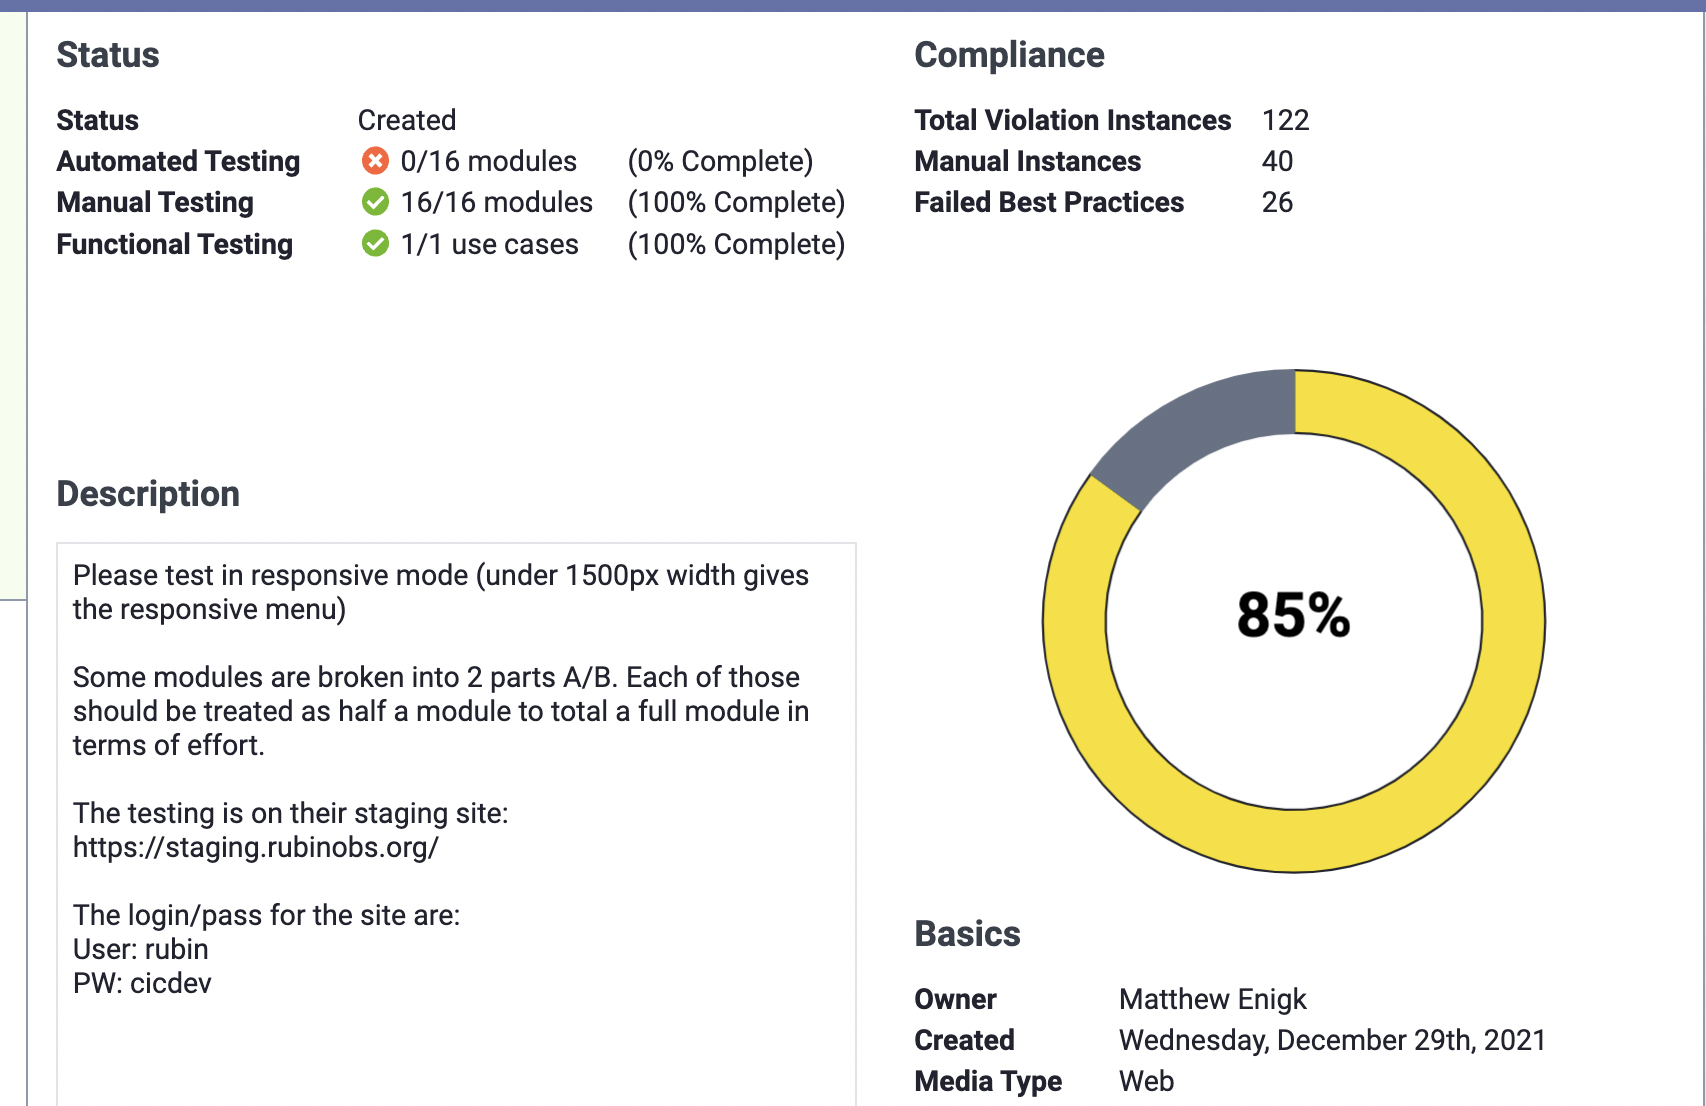
\includegraphics[width=3.12500in]{jira_imgs/2722.png}

}
\hdashrule[0.5ex]{\textwidth}{1pt}{3mm}
  Expected Result \\
{\footnotesize
Reports give a clear sense of the magnitude and severity of
accessibility related issues.

}

\begin{tabular}{p{2cm}}
\toprule
Step 2  \\ \hline
\end{tabular}
 Description \\
{\footnotesize
Observe the highest impact changes (i.e. changes resulting in
remediation of the largest number of violation occurrences addressed,
and/or the most severe violations) are
\href{https://github.com/orgs/lsst-epo/projects/1/views/9}{logged as
github issues}~

}
\hdashrule[0.5ex]{\textwidth}{1pt}{3mm}
  Expected Result \\
{\footnotesize
Report results have been reflected in github issues

}

\begin{tabular}{p{2cm}}
\toprule
Step 3  \\ \hline
\end{tabular}
 Description \\
{\footnotesize
Observe all gitub issues are marked as done, and have commits/PRs and/or
comments detailing steps taken to address the issues

}
\hdashrule[0.5ex]{\textwidth}{1pt}{3mm}
  Expected Result \\
{\footnotesize
All github issues are done

}

\begin{tabular}{p{2cm}}
\toprule
Step 4  \\ \hline
\end{tabular}
 Description \\
{\footnotesize
Inspect
\href{https://jira.lsstcorp.org/rest/tests/1.0/attachment/3160}{report
detailing the current number and variety of violations (i.e. after
remediation)}, and an overall aggregate ``score'' for EPO website to
conform with WCAG 2.0 Level AA requirements.~\\
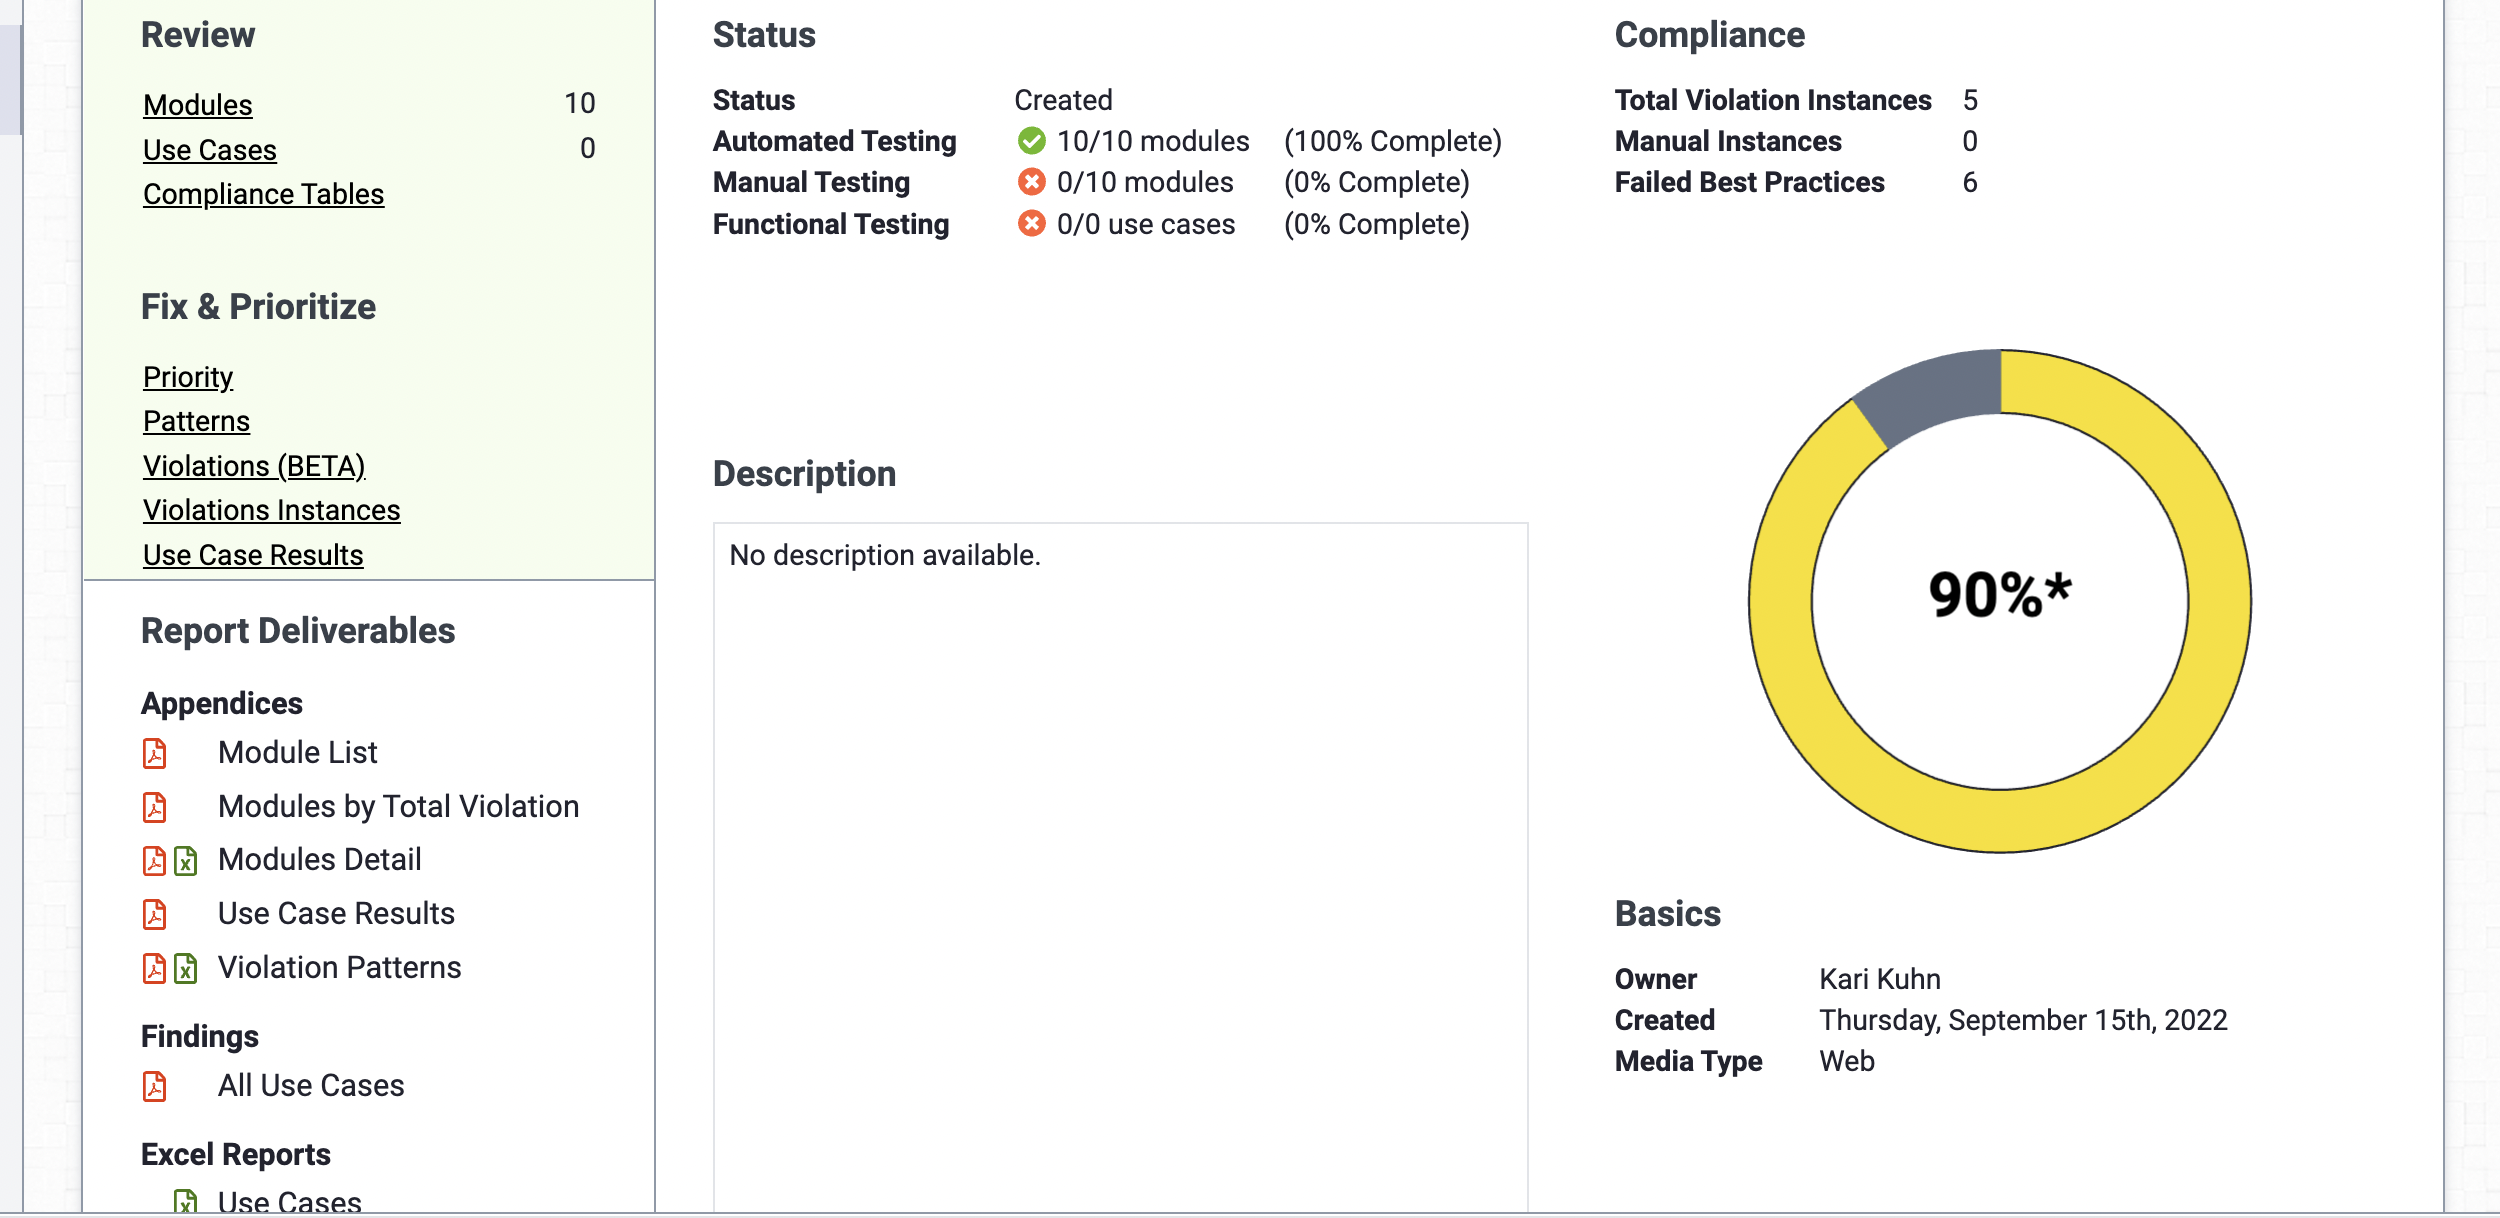
\includegraphics[width=3.12500in]{jira_imgs/3161.png}

}
\hdashrule[0.5ex]{\textwidth}{1pt}{3mm}
  Expected Result \\
{\footnotesize
Reports give a clear sense of the magnitude and severity of
accessibility related issues.

}

\paragraph{ LVV-T1889 - Inspect Operations website for media gallery }\mbox{}\\

Version \textbf{1}.
Open  \href{https://jira.lsstcorp.org/secure/Tests.jspa#/testCase/LVV-T1889}{\textit{ LVV-T1889 } }
test case in Jira.

Visually inspect that a gallery featuring Rubin Observatory multimedia
assets exists and can be viewed.

\textbf{ Preconditions}:\\


Final comment:\\


Detailed steps :

\begin{tabular}{p{2cm}}
\toprule
Step 1  \\ \hline
\end{tabular}
 Description \\
{\footnotesize
Visit \url{https://rubinobs.org/gallery} and visually inspect that the
Gallery exists

}
\hdashrule[0.5ex]{\textwidth}{1pt}{3mm}
  Expected Result \\
{\footnotesize
page loads free of errors

}

\begin{tabular}{p{2cm}}
\toprule
Step 2  \\ \hline
\end{tabular}
 Description \\
{\footnotesize
Confirm that the media assets can be browsed in the grid layout

}
\hdashrule[0.5ex]{\textwidth}{1pt}{3mm}
  Expected Result \\
{\footnotesize
Media assets are browsable

}

\begin{tabular}{p{2cm}}
\toprule
Step 3  \\ \hline
\end{tabular}
 Description \\
{\footnotesize
Enter ``dome'' into the gallery search bar

}
\hdashrule[0.5ex]{\textwidth}{1pt}{3mm}
  Expected Result \\
{\footnotesize
Search results include assets tagged, or with metadata that includes the
term ``dome''

}

\begin{tabular}{p{2cm}}
\toprule
Step 4  \\ \hline
\end{tabular}
 Description \\
{\footnotesize
Click on any asset thumbnail in the gallery view

}
\hdashrule[0.5ex]{\textwidth}{1pt}{3mm}
  Expected Result \\
{\footnotesize
Gallery asset detail page loads free of errors

}

\begin{tabular}{p{2cm}}
\toprule
Step 5  \\ \hline
\end{tabular}
 Description \\
{\footnotesize
Click the ``Download Image'' button

}
\hdashrule[0.5ex]{\textwidth}{1pt}{3mm}
  Expected Result \\
{\footnotesize
Redirected to image url ready for copy/paste use, or to be right clicked
and downloaded to your computer

}

\paragraph{ LVV-T1943 - Inspect Rubin Ops public site gallery slideshow }\mbox{}\\

Version \textbf{1}.
Open  \href{https://jira.lsstcorp.org/secure/Tests.jspa#/testCase/LVV-T1943}{\textit{ LVV-T1943 } }
test case in Jira.

Successfully visually identify how lists have been incorporated in the
Rubin Ops public site

\textbf{ Preconditions}:\\


Final comment:\\


Detailed steps :

\begin{tabular}{p{2cm}}
\toprule
Step 1  \\ \hline
\end{tabular}
 Description \\
{\footnotesize
Visit \url{https://rubinobs.org/gallery/slideshows}~

}
\hdashrule[0.5ex]{\textwidth}{1pt}{3mm}
  Expected Result \\
{\footnotesize
A list of all slideshows appears for the test

}

\begin{tabular}{p{2cm}}
\toprule
Step 2  \\ \hline
\end{tabular}
 Description \\
{\footnotesize
Click on the Slideshow ``Welcome to Rubin Observatory'' ~first
slideshow.~

}
\hdashrule[0.5ex]{\textwidth}{1pt}{3mm}
  Expected Result \\
{\footnotesize
The first slide of the gallery slideshow loads.~

}

\begin{tabular}{p{2cm}}
\toprule
Step 3  \\ \hline
\end{tabular}
 Description \\
{\footnotesize
Click through all slides to confirm listicle items all load free of
errors

}
\hdashrule[0.5ex]{\textwidth}{1pt}{3mm}
  Expected Result \\
{\footnotesize
Each slide loads and shows the next item in the list of content for the
user.~

}

\paragraph{ LVV-T1929 - Inspect that the multimedia gallery contains 3D models. }\mbox{}\\

Version \textbf{1}.
Open  \href{https://jira.lsstcorp.org/secure/Tests.jspa#/testCase/LVV-T1929}{\textit{ LVV-T1929 } }
test case in Jira.

To inspect that 3D models in a commonly accepted format is provided in
the EPO multimedia gallery

\textbf{ Preconditions}:\\


Final comment:\\


Detailed steps :

\begin{tabular}{p{2cm}}
\toprule
Step 1  \\ \hline
\end{tabular}
 Description \\
{\footnotesize
Visit
\href{https://rubin.canto.com/v/gallery/library?display=fitView\&viewIndex=2\&filter=\%7B\%22tagLiteral\%22:\%22CAD\%22\%7D}{this
gallery page}, pre-filtered to show available CAD files in Google Chrome

}
\hdashrule[0.5ex]{\textwidth}{1pt}{3mm}
  Expected Result \\
{\footnotesize
Page loads free of errors

}

\begin{tabular}{p{2cm}}
\toprule
Step 2  \\ \hline
\end{tabular}
 Description \\
{\footnotesize
Visually inspect that 3D models are provided in the EPO multimedia
gallery.

}
\hdashrule[0.5ex]{\textwidth}{1pt}{3mm}
  Expected Result \\
{\footnotesize
Gallery grid should be populated exclusively with 3D files thumbnails

}

\begin{tabular}{p{2cm}}
\toprule
Step 3  \\ \hline
\end{tabular}
 Description \\
{\footnotesize
Click on one of the 3D model thumbnails in the Gallery grid to visit its
Gallery Item Details page

}
\hdashrule[0.5ex]{\textwidth}{1pt}{3mm}
  Expected Result \\
{\footnotesize
Page loads free of errors

}

\begin{tabular}{p{2cm}}
\toprule
Step 4  \\ \hline
\end{tabular}
 Description \\
{\footnotesize
Click through the download button to save to your device

}
\hdashrule[0.5ex]{\textwidth}{1pt}{3mm}
  Expected Result \\
{\footnotesize
File successfully downloads onto your computer~

}

\begin{tabular}{p{2cm}}
\toprule
Step 5  \\ \hline
\end{tabular}
 Description \\
{\footnotesize
Visually inspect that the 3D model is provided in a commonly accepted
format.

}
\hdashrule[0.5ex]{\textwidth}{1pt}{3mm}
  Test Data \\
 {\footnotesize
Pre-defined commonly accepted format~

}
\hdashrule[0.5ex]{\textwidth}{1pt}{3mm}
  Expected Result \\
{\footnotesize
The models are in the pre-specified format.~

}

\paragraph{ LVV-T1928 - Inspect multimedia gallery includes images assets in flat and fisheye
formats }\mbox{}\\

Version \textbf{1}.
Open  \href{https://jira.lsstcorp.org/secure/Tests.jspa#/testCase/LVV-T1928}{\textit{ LVV-T1928 } }
test case in Jira.

Inspect that the EPO multimedia gallery is inspected to have images in
both flat and fisheye formats.

\textbf{ Preconditions}:\\


Final comment:\\


Detailed steps :

\begin{tabular}{p{2cm}}
\toprule
Step 1  \\ \hline
\end{tabular}
 Description \\
{\footnotesize
Visit \href{https://rubinobs.com/gallery}{the rubin gallery page} in
Google Chrome

}
\hdashrule[0.5ex]{\textwidth}{1pt}{3mm}
  Expected Result \\
{\footnotesize
Page loads free of errors

}

\begin{tabular}{p{2cm}}
\toprule
Step 2  \\ \hline
\end{tabular}
 Description \\
{\footnotesize
Visually inspect that the EPO multimedia gallery contains Flat images.
~\href{https://rubin.canto.com/v/gallery/album/HDSNU?display=curatedView\&viewIndex=2\&column=image\&id=kcg0oujc9h1q3dobm135pjg91j}{This
is one such example}.

}
\hdashrule[0.5ex]{\textwidth}{1pt}{3mm}
  Expected Result \\
{\footnotesize
The gallery grid will show a mix of thumbnails for all kinds of image
formats, flat images included

}

\begin{tabular}{p{2cm}}
\toprule
Step 3  \\ \hline
\end{tabular}
 Description \\
{\footnotesize
Visually inspect that the EPO multimedia gallery contains fisheye
images.
~\href{https://rubin.canto.com/v/gallery/album/HDSNU?display=curatedView\&viewIndex=2\&from=curatedView\&filter=\%7B\%22tagLiteral\%22:\%22Fisheye\%22\%7D}{Here
are the Gallery Assets pre-filtered for Fisheye format}

}
\hdashrule[0.5ex]{\textwidth}{1pt}{3mm}
  Expected Result \\
{\footnotesize
The gallery grid will show a mix of thumbnails for all kinds of image
formats, fisheye images included

}

\paragraph{ LVV-T2584 - IMERSA AFDI Dome Master metadata saved to Fulldome (Planeteria) videos }\mbox{}\\

Version \textbf{1}.
Open  \href{https://jira.lsstcorp.org/secure/Tests.jspa#/testCase/LVV-T2584}{\textit{ LVV-T2584 } }
test case in Jira.

To test full dome video for presence of metadata.

\textbf{ Preconditions}:\\


Final comment:\\


Detailed steps :

\begin{tabular}{p{2cm}}
\toprule
Step 1  \\ \hline
\end{tabular}
 Description \\
{\footnotesize
Visit
\href{https://rubin.canto.com/v/RubinPlanetariumAssets/landing}{Rubin
Planetarium Assets Landing Page} in Google Chrome

}
\hdashrule[0.5ex]{\textwidth}{1pt}{3mm}
  Expected Result \\
{\footnotesize
Full dome planetarium video details page loads free of errors

}

\begin{tabular}{p{2cm}}
\toprule
Step 2  \\ \hline
\end{tabular}
 Description \\
{\footnotesize
Checkout
\href{https://rubin.canto.com/v/RubinPlanetariumAssets/album/HGA21}{one
of the Fulldome videos}

}
\hdashrule[0.5ex]{\textwidth}{1pt}{3mm}
  Expected Result \\
{\footnotesize

}

\begin{tabular}{p{2cm}}
\toprule
Step 3  \\ \hline
\end{tabular}
 Description \\
{\footnotesize
Click the ``Download'' button in the bottom right corner of each
available asset (image sequence zip, suggested narration pdf, video
preview, and metadata file)

}
\hdashrule[0.5ex]{\textwidth}{1pt}{3mm}
  Expected Result \\
{\footnotesize
Files downloads to your computer no prob

}

\begin{tabular}{p{2cm}}
\toprule
Step 4  \\ \hline
\end{tabular}
 Description \\
{\footnotesize
Inspect the fulldome video preview plays as expected

}
\hdashrule[0.5ex]{\textwidth}{1pt}{3mm}
  Expected Result \\
{\footnotesize
video preview plays

}

\begin{tabular}{p{2cm}}
\toprule
Step 5  \\ \hline
\end{tabular}
 Description \\
{\footnotesize
Visually inspect that details in the metadata file are consistent
~include any required
\href{http://www.imersa.org/images/standards/AFDI\%20standards\%20v1.0.pdf}{IMERSA
AFDI Dome Master metadata fields}

}
\hdashrule[0.5ex]{\textwidth}{1pt}{3mm}
  Test Data \\
 {\footnotesize
XML samples of fulldome fields:
\href{https://jira.lsstcorp.org/rest/tests/1.0/attachment/3162}{samplefulldomexml.dml}

}
\hdashrule[0.5ex]{\textwidth}{1pt}{3mm}
  Expected Result \\
{\footnotesize
IMERSA AFDI Dome Master metadata fields are present and have values
where applicable

}

\begin{tabular}{p{2cm}}
\toprule
Step 6  \\ \hline
\end{tabular}
 Description \\
{\footnotesize
Open narration pdf and confirm its contents align with provided video

}
\hdashrule[0.5ex]{\textwidth}{1pt}{3mm}
  Expected Result \\
{\footnotesize
Timecode matches, and attributions and contents are appropriate to the
fulldome video

}

\begin{tabular}{p{2cm}}
\toprule
Step 7  \\ \hline
\end{tabular}
 Description \\
{\footnotesize
Unzip image sequence and observe it is a directory of video frames
numbered in sequence

}
\hdashrule[0.5ex]{\textwidth}{1pt}{3mm}
  Expected Result \\
{\footnotesize
Image files have sequential file names and consistent file types

}

\paragraph{ LVV-T1925 - Inspect metadata of EPO assets excluding telescope images and
planetarium videos }\mbox{}\\

Version \textbf{1}.
Open  \href{https://jira.lsstcorp.org/secure/Tests.jspa#/testCase/LVV-T1925}{\textit{ LVV-T1925 } }
test case in Jira.

Inspect that the specified metadata exist for the appropriate assets
that are neither telescope images or planetarium videos

\textbf{ Preconditions}:\\


Final comment:\\


Detailed steps :

\begin{tabular}{p{2cm}}
\toprule
Step 1  \\ \hline
\end{tabular}
 Description \\
{\footnotesize
Consider that image metadata should include, at a minimum ``Type, Title,
Description, Credit, MetadataDate, MetadataVersion, PublisherID,
ResourceID, ResourceURL, DateCreated (in ISO 8601 notation), and
UsageTerms''

}
\hdashrule[0.5ex]{\textwidth}{1pt}{3mm}
  Expected Result \\
{\footnotesize
Take note of these fields as you'll be referencing them in the next
steps

}

\begin{tabular}{p{2cm}}
\toprule
Step 2  \\ \hline
\end{tabular}
 Description \\
{\footnotesize
Visit
\href{https://rubin.canto.com/v/gallery/album/HDSNU?display=curatedView\&viewIndex=2\&column=image\&id=0br386177p6l19tftvetlrj361}{this
Gallery Asset page} in Google Chrome

}
\hdashrule[0.5ex]{\textwidth}{1pt}{3mm}
  Expected Result \\
{\footnotesize
Image details page loads free of errors

}

\begin{tabular}{p{2cm}}
\toprule
Step 3  \\ \hline
\end{tabular}
 Description \\
{\footnotesize
Right click and ``save as image'' to your device, or click through
``Download Image'' button and then right click and ``save as image'' to
your device

}
\hdashrule[0.5ex]{\textwidth}{1pt}{3mm}
  Expected Result \\
{\footnotesize
File downloads to your computer no prob

}

\begin{tabular}{p{2cm}}
\toprule
Step 4  \\ \hline
\end{tabular}
 Description \\
{\footnotesize
Visit \href{http://exif.tools}{exif.tools} in Google Chrome.

}
\hdashrule[0.5ex]{\textwidth}{1pt}{3mm}
  Expected Result \\
{\footnotesize
Page loads free of errors, presenting a simple file upload interface

}

\begin{tabular}{p{2cm}}
\toprule
Step 5  \\ \hline
\end{tabular}
 Description \\
{\footnotesize
Upload the image you saved and click ``Upload''

}
\hdashrule[0.5ex]{\textwidth}{1pt}{3mm}
  Expected Result \\
{\footnotesize
Image uploads successfully; no error messages on upload; New page with
list of all image metadata in a table

}

\begin{tabular}{p{2cm}}
\toprule
Step 6  \\ \hline
\end{tabular}
 Description \\
{\footnotesize
Scroll through metadata table and identify the default fields (as
provided in step 1) are used in the AVM specific fields and have value

}
\hdashrule[0.5ex]{\textwidth}{1pt}{3mm}
  Expected Result \\
{\footnotesize
Default fields and value align with inspected metadata

}

\paragraph{ LVV-T1924 - Inspect telescope images in the multimedia gallery for the appropriate
metadata. }\mbox{}\\

Version \textbf{1}.
Open  \href{https://jira.lsstcorp.org/secure/Tests.jspa#/testCase/LVV-T1924}{\textit{ LVV-T1924 } }
test case in Jira.

Visually confirm that the metadata in the correct format are provided
for images in the Rubin multimedia gallery.

\textbf{ Preconditions}:\\


Final comment:\\


Detailed steps :

\begin{tabular}{p{2cm}}
\toprule
Step 1  \\ \hline
\end{tabular}
 Description \\
{\footnotesize
Consider that image metadata should include, at a minimum,
Spatial.CoordinateFrame, Spatial.ReferenceValue,
Spatial.ReferenceDimension, Spatial.ReferencePixel, Spatial.Scale,
Spatial.Rotation, and Spatial.CoordsystemProjection

}
\hdashrule[0.5ex]{\textwidth}{1pt}{3mm}
  Expected Result \\
{\footnotesize
Take note of these fields as you'll be referencing them in the next
steps

}

\begin{tabular}{p{2cm}}
\toprule
Step 2  \\ \hline
\end{tabular}
 Description \\
{\footnotesize
Visit
\href{https://rubin.canto.com/v/gallery/library?keyword=deep\&viewIndex=2\&display=fitView\&from=curatedView\&column=image\&id=ai03ln71vt1bl84fu316jig871}{this
gallery asset page} in Google Chrome\\[2\baselineskip]

}
\hdashrule[0.5ex]{\textwidth}{1pt}{3mm}
  Expected Result \\
{\footnotesize
Gallery Image Details page loads free of errors

}

\begin{tabular}{p{2cm}}
\toprule
Step 3  \\ \hline
\end{tabular}
 Description \\
{\footnotesize
Click the download button and select your desired image quality to
download to your computer

}
\hdashrule[0.5ex]{\textwidth}{1pt}{3mm}
  Expected Result \\
{\footnotesize
File downloads to your computer no prob

}

\begin{tabular}{p{2cm}}
\toprule
Step 4  \\ \hline
\end{tabular}
 Description \\
{\footnotesize
Visit \href{http://exif.tools}{exif.tools} in Google Chrome

}
\hdashrule[0.5ex]{\textwidth}{1pt}{3mm}
  Expected Result \\
{\footnotesize
Image uploads successfully; no error messages on upload; New page with
list of all image metadata in a table

}

\begin{tabular}{p{2cm}}
\toprule
Step 5  \\ \hline
\end{tabular}
 Description \\
{\footnotesize
Scroll through metadata table and identify AVM specific fields with
values appropriate to image subject

}
\hdashrule[0.5ex]{\textwidth}{1pt}{3mm}
  Expected Result \\
{\footnotesize
AVM info present in metadata table

}

\subsection{Test Cycle LVV-C223 }

Open test cycle {\it \href{https://jira.lsstcorp.org/secure/Tests.jspa#/testrun/LVV-C223}{EPO October Verification}} in Jira.

Test Cycle name: EPO October Verification\\
Status: Done

These test cases are the few that can not be verified as part of the
original September campaign by EPO.~

\subsubsection{Software Version/Baseline}
Not provided.

\subsubsection{Configuration}
Not provided.

\subsubsection{Test Cases in LVV-C223 Test Cycle}

\paragraph{ LVV-T2722 - Verify that images curated via the TAP -\textgreater{} Butler
-\textgreater{} AWF workflow can be sent to Zooniverse for the creation
of a subject set based on the curated image data }\mbox{}\\

Version \textbf{1}.
Open  \href{https://jira.lsstcorp.org/secure/Tests.jspa#/testCase/LVV-T2722}{\textit{ LVV-T2722 } }
test case in Jira.

Verify that images curated via the TAP -\textgreater{} Butler
-\textgreater{} AWF workflow can be sent to Zooniverse for the creation
of a subject set based on the curated image data

\textbf{ Preconditions}:\\


Final comment:\\


Detailed steps :

\begin{tabular}{p{2cm}}
\toprule
Step 1  \\ \hline
\end{tabular}
 Description \\
{\footnotesize
On a device connected to the internet, such as a laptop, open a web
browser application.

}
\hdashrule[0.5ex]{\textwidth}{1pt}{3mm}
  Expected Result \\
{\footnotesize
A web browser opens on the device.

}

\begin{tabular}{p{2cm}}
\toprule
Step 2  \\ \hline
\end{tabular}
 Description \\
{\footnotesize
Go to the URL: https://data.lsst.cloud/nb

}
\hdashrule[0.5ex]{\textwidth}{1pt}{3mm}
  Expected Result \\
{\footnotesize
The Login page, the Server Options page, or the Notebook Aspect will
load in the browser.

}

\begin{tabular}{p{2cm}}
\toprule
Step 3  \\ \hline
\end{tabular}
 Description \\
{\footnotesize
\textbf{Conditional:~}If the Login page loads, authenticate by
authorizing Github to login on your behalf.

}
\hdashrule[0.5ex]{\textwidth}{1pt}{3mm}
  Expected Result \\
{\footnotesize
The Server Options page loads in the browser

}

\begin{tabular}{p{2cm}}
\toprule
Step 4  \\ \hline
\end{tabular}
 Description \\
{\footnotesize
\textbf{Conditional:~}If the Server Options page loads, go with whatever
default values are already selected and click the orange ``Start''
button

}
\hdashrule[0.5ex]{\textwidth}{1pt}{3mm}
  Expected Result \\
{\footnotesize
The Notebook Aspect Jupyter Hub environment will load

}

\begin{tabular}{p{2cm}}
\toprule
Step 5  \\ \hline
\end{tabular}
 Description \\
{\footnotesize
Run the cell to log into the Zooniverse platform

}
\hdashrule[0.5ex]{\textwidth}{1pt}{3mm}
  Expected Result \\
{\footnotesize
The user is authenticated into the Zooniverse platform

}

\begin{tabular}{p{2cm}}
\toprule
Step 6  \\ \hline
\end{tabular}
 Description \\
{\footnotesize
Proceed through the tutorial notebook to activate the Citizen Science
SDK cells

}
\hdashrule[0.5ex]{\textwidth}{1pt}{3mm}
  Expected Result \\
{\footnotesize
The SDK cells are activated

}

\begin{tabular}{p{2cm}}
\toprule
Step 7  \\ \hline
\end{tabular}
 Description \\
{\footnotesize
Use the TAP query service to query for points of interest

}
\hdashrule[0.5ex]{\textwidth}{1pt}{3mm}
  Expected Result \\
{\footnotesize
The TAP query results are returned with records containing points of
interest

}

\begin{tabular}{p{2cm}}
\toprule
Step 8  \\ \hline
\end{tabular}
 Description \\
{\footnotesize
Use the results of the TAP query to use the Butler to retrieve image
data related to the points of interest

}
\hdashrule[0.5ex]{\textwidth}{1pt}{3mm}
  Expected Result \\
{\footnotesize
The Butler service returns the image data

}

\begin{tabular}{p{2cm}}
\toprule
Step 9  \\ \hline
\end{tabular}
 Description \\
{\footnotesize
Use the SDK cells, which contain functions that make use of the DM AFW
tools, to produce PNGs and save them to the filesystem

}
\hdashrule[0.5ex]{\textwidth}{1pt}{3mm}
  Expected Result \\
{\footnotesize
The PNGs are created and saved to the filesystem

}

\begin{tabular}{p{2cm}}
\toprule
Step 10  \\ \hline
\end{tabular}
 Description \\
{\footnotesize
Use the proceeding cells to give your subject set a name

}
\hdashrule[0.5ex]{\textwidth}{1pt}{3mm}
  Expected Result \\
{\footnotesize
A name is given to the new subject set

}

\begin{tabular}{p{2cm}}
\toprule
Step 11  \\ \hline
\end{tabular}
 Description \\
{\footnotesize
Call the~\textbf{send\_data()} Citizen Science SDK to send the cutouts
to Zooniverse

}
\hdashrule[0.5ex]{\textwidth}{1pt}{3mm}
  Expected Result \\
{\footnotesize
The data is sent to Zooniverse and a message appears notifying the user
as such

}

\begin{tabular}{p{2cm}}
\toprule
Step 12  \\ \hline
\end{tabular}
 Description \\
{\footnotesize
Go onto the Zooniverse platform and verify that the data was transferred
successfully

}
\hdashrule[0.5ex]{\textwidth}{1pt}{3mm}
  Expected Result \\
{\footnotesize
The user verifies that the new subject set appears on the Zooniverse
platform containing the image data they curated.

}

\paragraph{ LVV-T2689 - Demonstrate citizen science pipeline with two scientists }\mbox{}\\

Version \textbf{1}.
Open  \href{https://jira.lsstcorp.org/secure/Tests.jspa#/testCase/LVV-T2689}{\textit{ LVV-T2689 } }
test case in Jira.

The EPO Citizen Science pipeline should be usable without moderation
from a member of the EPO team. This test will verify with two different
people that they can use our notebook to successfully send data from the
RSP to a Zooniverse project.~\\
The Precursor Citizen Science Projects requirement shall be verified by
demonstration. A representative for each citizen science project shall
document a demonstration of how their project was successfully provided
data starting from a data collection in the RSP to use in a Zooniverse
project.

\textbf{ Preconditions}:\\


Final comment:\\


Detailed steps :

\begin{tabular}{p{2cm}}
\toprule
Step 1  \\ \hline
\end{tabular}
 Description \\
{\footnotesize
Inspect pdf of executed citizen science notebook by astronomer 1.~

}
\hdashrule[0.5ex]{\textwidth}{1pt}{3mm}
  Expected Result \\
{\footnotesize
The pdf shows the EPO citizen science notebook successfully sent 100
objects to the Zooniverse.~

}

\begin{tabular}{p{2cm}}
\toprule
Step 2  \\ \hline
\end{tabular}
 Description \\
{\footnotesize
Inspect screenshot of the Zooniverse project builder too for astronomer
1.

}
\hdashrule[0.5ex]{\textwidth}{1pt}{3mm}
  Expected Result \\
{\footnotesize
The screenshot shows the subject set named in the citizen science
notebook is associated with the correct project on the Zooniverese
site.~

}

\begin{tabular}{p{2cm}}
\toprule
Step 3  \\ \hline
\end{tabular}
 Description \\
{\footnotesize
Inspect pdf of executed citizen science notebook by astronomer 2.

}
\hdashrule[0.5ex]{\textwidth}{1pt}{3mm}
  Expected Result \\
{\footnotesize
The pdf shows the EPO citizen science notebook successfully sent 100
objects to the Zooniverse.~

}

\begin{tabular}{p{2cm}}
\toprule
Step 4  \\ \hline
\end{tabular}
 Description \\
{\footnotesize
Inspect screenshot of the Zooniverse project builder too for astronomer
2.

}
\hdashrule[0.5ex]{\textwidth}{1pt}{3mm}
  Expected Result \\
{\footnotesize
The screenshot shows the subject set named in the citizen science
notebook is associated with the correct project on the Zooniverese
site.~

}

\paragraph{ LVV-T2008 - Identify fulldome projection of the night sky in EPO media gallery }\mbox{}\\

Version \textbf{1}.
Open  \href{https://jira.lsstcorp.org/secure/Tests.jspa#/testCase/LVV-T2008}{\textit{ LVV-T2008 } }
test case in Jira.

Identify fulldome projection of the LSST night sky. This requirement is
considered successful when a planetarium video of the night sky is
successfully played from the gallery.

\textbf{ Preconditions}:\\


Final comment:\\See the attached screen recording in
docushare:~\href{https://docushare.lsstcorp.org/docushare/dsweb/Get/Document-43309/Screen\%20Recording\%202022-10-21\%20at\%202.17.30\%20PM.mov}{\textbf{Screen
Recording 2022-10-21 at 2.17.30 PM.mov}}


Detailed steps :

\begin{tabular}{p{2cm}}
\toprule
Step 1  \\ \hline
\end{tabular}
 Description \\
{\footnotesize
Visit this
\href{https://rubin.canto.com/v/RubinPlanetariumAssets/album/S35P1?display=fitView\&viewIndex=2\&from=fitView\&column=video\&id=608u0g5qhh19b7t2n7gd9oud5s}{fulldome
night sky video page} in Chrome

}
\hdashrule[0.5ex]{\textwidth}{1pt}{3mm}
  Expected Result \\
{\footnotesize
Page loads free of errors

}

\begin{tabular}{p{2cm}}
\toprule
Step 2  \\ \hline
\end{tabular}
 Description \\
{\footnotesize
Use provided UI to play the video.~ Observe it is fulldome (fisheye) and
depicts the night sky over the Rubin observatory site

}
\hdashrule[0.5ex]{\textwidth}{1pt}{3mm}
  Expected Result \\
{\footnotesize
The video plays a fulldome sky projection.

}

\paragraph{ LVV-T1930 - Inspect 3D solar system model on EPO website }\mbox{}\\

Version \textbf{1}.
Open  \href{https://jira.lsstcorp.org/secure/Tests.jspa#/testCase/LVV-T1930}{\textit{ LVV-T1930 } }
test case in Jira.

To visually inspect that a 3D solar system model is available on the
website.

\textbf{ Preconditions}:\\


Final comment:\\


Detailed steps :

\begin{tabular}{p{2cm}}
\toprule
Step 1  \\ \hline
\end{tabular}
 Description \\
{\footnotesize
Visually inspect \href{https://vera-rubin.netlify.app/}{the EPO 3D solar
system model} is available.

}
\hdashrule[0.5ex]{\textwidth}{1pt}{3mm}
  Expected Result \\
{\footnotesize
The website contains the 3D solar system model.~

}

\paragraph{ LVV-T2569 - Inspect availability of Spanish language Educational Activities }\mbox{}\\

Version \textbf{1}.
Open  \href{https://jira.lsstcorp.org/secure/Tests.jspa#/testCase/LVV-T2569}{\textit{ LVV-T2569 } }
test case in Jira.

To Inspect availability of Spanish language Educational Activities.

\textbf{ Preconditions}:\\


Final comment:\\


Detailed steps :

\begin{tabular}{p{2cm}}
\toprule
Step 1  \\ \hline
\end{tabular}
 Description \\
{\footnotesize
Visit \url{https://surveyingthesolarsystem.netlify.app/es}~in Chrome to
see the Spanish version of the Surveying the Solar System investigation,
one example of EPO's education activities

}
\hdashrule[0.5ex]{\textwidth}{1pt}{3mm}
  Expected Result \\
{\footnotesize
First page of the Surveying the Solar System Investigation loads free of
errors

}

\begin{tabular}{p{2cm}}
\toprule
Step 2  \\ \hline
\end{tabular}
 Description \\
{\footnotesize
Navigate through any number of questions and pages

}
\hdashrule[0.5ex]{\textwidth}{1pt}{3mm}
  Expected Result \\
{\footnotesize
Observe all text and image content are appropriate for a Spanish
speaking audience

}

\paragraph{ LVV-T2568 - Inspect availability of Spanish language Educational Materials }\mbox{}\\

Version \textbf{1}.
Open  \href{https://jira.lsstcorp.org/secure/Tests.jspa#/testCase/LVV-T2568}{\textit{ LVV-T2568 } }
test case in Jira.

The objective of this test case is to inspect availability of Spanish
language Educational Materials

\textbf{ Preconditions}:\\


Final comment:\\See the attached docushare
\href{https://docushare.lsst.org/docushare/dsweb/Get/Document-43122/Screen\%20Recording\%202022-11-04\%20at\%203.53.24\%20PM.mov}{screen
recording}.~


Detailed steps :

\begin{tabular}{p{2cm}}
\toprule
Step 1  \\ \hline
\end{tabular}
 Description \\
{\footnotesize
Visit https://rubinobs.org/es/for-educators/educators in Chrome and
browse any number of pages to verify comparable content is available in
english and spanish

}
\hdashrule[0.5ex]{\textwidth}{1pt}{3mm}
  Expected Result \\
{\footnotesize
Loads the Spanish version of the
~https://rubinobs.org/es/for-educators/educators

}

\paragraph{ LVV-T1887 - Inspect availability of Spanish language EPO materials }\mbox{}\\

Version \textbf{1}.
Open  \href{https://jira.lsstcorp.org/secure/Tests.jspa#/testCase/LVV-T1887}{\textit{ LVV-T1887 } }
test case in Jira.

Inspect that core EPO materials for the Operations website and the
education program are translated and published in Spanish.

\textbf{ Preconditions}:\\


Final comment:\\See the attached docushare
\href{https://docushare.lsst.org/docushare/dsweb/Get/Document-43123/Screen\%20Recording\%202022-11-04\%20at\%203.58.44\%20PM.mov}{screen
recording}.


Detailed steps :

\begin{tabular}{p{2cm}}
\toprule
Step 1  \\ \hline
\end{tabular}
 Description \\
{\footnotesize
Visit \href{http://rubinobs.org}{rubinobs.org} in any modern web
browsers (e.g. Chrome, Firefox, Safari, Edge, etc.)

}
\hdashrule[0.5ex]{\textwidth}{1pt}{3mm}
  Expected Result \\
{\footnotesize
Loads the Rubin Ops homepage

}

\begin{tabular}{p{2cm}}
\toprule
Step 2  \\ \hline
\end{tabular}
 Description \\
{\footnotesize
Visit \url{http://rubinobs.org/es} in any modern web browsers (e.g.
Chrome, Firefox, Safari, Edge, etc.)\\[2\baselineskip]

}
\hdashrule[0.5ex]{\textwidth}{1pt}{3mm}
  Expected Result \\
{\footnotesize
Loads the Spanish version of the Rubin Ops homepage

}

\begin{tabular}{p{2cm}}
\toprule
Step 3  \\ \hline
\end{tabular}
 Description \\
{\footnotesize
Click the language toggle in the top right corner of the page (on mobile
is at the top of the hamburger dropdown menu)

}
\hdashrule[0.5ex]{\textwidth}{1pt}{3mm}
  Expected Result \\
{\footnotesize
If on \url{http://rubinobs.org/es} will switch to the English version of
the homepage: \url{http://rubinobs.org}. ~If on
\url{http://rubinobs.org} will switch to the Spanish version of the
homepage:~\url{http://rubinobs.org/es}

}

\begin{tabular}{p{2cm}}
\toprule
Step 4  \\ \hline
\end{tabular}
 Description \\
{\footnotesize
Inspect the translated materials for conceptual similarities.

}
\hdashrule[0.5ex]{\textwidth}{1pt}{3mm}
  Expected Result \\
{\footnotesize
Language-specific content may not, and need not, be a literal 1:1
translation. ~The language-specific content should be appropriate to
English and Spanish speaking audiences, especially US and Chilean
audiences.

}

\paragraph{ LVV-T1884 - Inspect bios exist on Operations website }\mbox{}\\

Version \textbf{1}.
Open  \href{https://jira.lsstcorp.org/secure/Tests.jspa#/testCase/LVV-T1884}{\textit{ LVV-T1884 } }
test case in Jira.

Confirm that the correct number of bios featuring personal vignettes are
included on the website by the end of transition into Operations.~

\textbf{ Preconditions}:\\


Final comment:\\See the docushare
\href{https://docushare.lsstcorp.org/docushare/dsweb/Get/Document-43048/Screen\%20Recording\%202022-10-21\%20at\%202.45.41\%20PM.mov}{screenshot}~.


Detailed steps :

\begin{tabular}{p{2cm}}
\toprule
Step 1  \\ \hline
\end{tabular}
 Description \\
{\footnotesize
Visit www.rubinobs.org/explore/voices/all-rubin-voices

}
\hdashrule[0.5ex]{\textwidth}{1pt}{3mm}
  Expected Result \\
{\footnotesize
The link takes the tester to the Rubin Voices webpage.~

}

\begin{tabular}{p{2cm}}
\toprule
Step 2  \\ \hline
\end{tabular}
 Description \\
{\footnotesize
Inspect that the collection that appears contains 12+ profiles of Rubin
Community members

}
\hdashrule[0.5ex]{\textwidth}{1pt}{3mm}
  Expected Result \\
{\footnotesize
The tester can visually confirm that 12+ profiles of Rubin Community
members

}

\begin{tabular}{p{2cm}}
\toprule
Step 3  \\ \hline
\end{tabular}
 Description \\
{\footnotesize
Inspect that these bio of Sarah Brough contains personal vignettes.

}
\hdashrule[0.5ex]{\textwidth}{1pt}{3mm}
  Test Data \\
 {\footnotesize
https://rubinobs.org/explore/staff/sarah-brough

}
\hdashrule[0.5ex]{\textwidth}{1pt}{3mm}
  Expected Result \\
{\footnotesize
Confirm that the bio of Sarah Brough contain personal vignettes relating
to the scientist being highlighted.

}

\begin{tabular}{p{2cm}}
\toprule
Step 4  \\ \hline
\end{tabular}
 Description \\
{\footnotesize
Inspect that these bio of Nushkia Chamba contains personal vignettes.

}
\hdashrule[0.5ex]{\textwidth}{1pt}{3mm}
  Test Data \\
 {\footnotesize
https://rubinobs.org/explore/staff/nushkia-chamba

}
\hdashrule[0.5ex]{\textwidth}{1pt}{3mm}
  Expected Result \\
{\footnotesize
Confirm that the bio of Nushkia Chamba contain personal vignettes
relating to the scientist being highlighted.

}

\begin{tabular}{p{2cm}}
\toprule
Step 5  \\ \hline
\end{tabular}
 Description \\
{\footnotesize
Inspect that these bio of Louise Edwards contains personal vignettes.

}
\hdashrule[0.5ex]{\textwidth}{1pt}{3mm}
  Test Data \\
 {\footnotesize
https://rubinobs.org/explore/staff/louise-edwards

}
\hdashrule[0.5ex]{\textwidth}{1pt}{3mm}
  Expected Result \\
{\footnotesize
Confirm that the bio of Louise Edwards contain personal vignettes
relating to the scientist being highlighted.

}

\begin{tabular}{p{2cm}}
\toprule
Step 6  \\ \hline
\end{tabular}
 Description \\
{\footnotesize
Inspect that these bio of Colin Orion Chandler contains personal
vignettes.

}
\hdashrule[0.5ex]{\textwidth}{1pt}{3mm}
  Test Data \\
 {\footnotesize
https://rubinobs.org/explore/staff/colin-orion-chandler

}
\hdashrule[0.5ex]{\textwidth}{1pt}{3mm}
  Expected Result \\
{\footnotesize
Confirm that the bio of Colin Orion Chandler contain personal vignettes
relating to the scientist being highlighted.

}

\begin{tabular}{p{2cm}}
\toprule
Step 7  \\ \hline
\end{tabular}
 Description \\
{\footnotesize
Inspect that these bio of Adam Snyder contains personal vignettes.

}
\hdashrule[0.5ex]{\textwidth}{1pt}{3mm}
  Test Data \\
 {\footnotesize
https://rubinobs.org/explore/staff/adam-snyder

}
\hdashrule[0.5ex]{\textwidth}{1pt}{3mm}
  Expected Result \\
{\footnotesize
Confirm that the bio of Adam Snyder contain personal vignettes relating
to the scientist being highlighted.

}

\begin{tabular}{p{2cm}}
\toprule
Step 8  \\ \hline
\end{tabular}
 Description \\
{\footnotesize
Inspect that these bio of Qingling Ni contains personal vignettes.

}
\hdashrule[0.5ex]{\textwidth}{1pt}{3mm}
  Test Data \\
 {\footnotesize
https://rubinobs.org/explore/staff/qingling-ni

}
\hdashrule[0.5ex]{\textwidth}{1pt}{3mm}
  Expected Result \\
{\footnotesize
Confirm that the bio of Qingling Ni contain personal vignettes relating
to the scientist being highlighted.

}

\begin{tabular}{p{2cm}}
\toprule
Step 9  \\ \hline
\end{tabular}
 Description \\
{\footnotesize
Inspect that these bio of Anais Moeller contains personal vignettes.

}
\hdashrule[0.5ex]{\textwidth}{1pt}{3mm}
  Test Data \\
 {\footnotesize
https://rubinobs.org/explore/staff/anais-moeller

}
\hdashrule[0.5ex]{\textwidth}{1pt}{3mm}
  Expected Result \\
{\footnotesize
Confirm that the bio of Anais Moeller contain personal vignettes
relating to the scientist being highlighted.

}

\begin{tabular}{p{2cm}}
\toprule
Step 10  \\ \hline
\end{tabular}
 Description \\
{\footnotesize
Inspect that these bio of Ardis Herrold contains personal vignettes.

}
\hdashrule[0.5ex]{\textwidth}{1pt}{3mm}
  Test Data \\
 {\footnotesize
https://rubinobs.org/explore/staff/ardis-herrold

}
\hdashrule[0.5ex]{\textwidth}{1pt}{3mm}
  Expected Result \\
{\footnotesize
Confirm that the bio of Ardis Herrold contain personal vignettes
relating to the scientist being highlighted.

}

\begin{tabular}{p{2cm}}
\toprule
Step 11  \\ \hline
\end{tabular}
 Description \\
{\footnotesize
Inspect that these bio of Bruno Quint contains personal vignettes.

}
\hdashrule[0.5ex]{\textwidth}{1pt}{3mm}
  Test Data \\
 {\footnotesize
https://rubinobs.org/explore/staff/bruno-quint

}
\hdashrule[0.5ex]{\textwidth}{1pt}{3mm}
  Expected Result \\
{\footnotesize
Confirm that the bio of Bruno Quint contain personal vignettes relating
to the scientist being highlighted.

}

\begin{tabular}{p{2cm}}
\toprule
Step 12  \\ \hline
\end{tabular}
 Description \\
{\footnotesize
Inspect that these bio of Christian Aganze contains personal vignettes.

}
\hdashrule[0.5ex]{\textwidth}{1pt}{3mm}
  Test Data \\
 {\footnotesize
https://rubinobs.org/explore/staff/christian-aganze

}
\hdashrule[0.5ex]{\textwidth}{1pt}{3mm}
  Expected Result \\
{\footnotesize
Confirm that the bio of Christian Aganze contain personal vignettes
relating to the scientist being highlighted.

}

\begin{tabular}{p{2cm}}
\toprule
Step 13  \\ \hline
\end{tabular}
 Description \\
{\footnotesize
Inspect that these bio of Sandrine Thomas contains personal vignettes.

}
\hdashrule[0.5ex]{\textwidth}{1pt}{3mm}
  Test Data \\
 {\footnotesize
https://rubinobs.org/explore/staff/sandrine-thomas

}
\hdashrule[0.5ex]{\textwidth}{1pt}{3mm}
  Expected Result \\
{\footnotesize
Confirm that the bio of Sandrine Thomas contain personal vignettes
relating to the scientist being highlighted.

}

\begin{tabular}{p{2cm}}
\toprule
Step 14  \\ \hline
\end{tabular}
 Description \\
{\footnotesize
Inspect that these bio of Somayeh Khakpash contains personal vignettes.

}
\hdashrule[0.5ex]{\textwidth}{1pt}{3mm}
  Test Data \\
 {\footnotesize
https://rubinobs.org/explore/staff/somayeh-khakpash

}
\hdashrule[0.5ex]{\textwidth}{1pt}{3mm}
  Expected Result \\
{\footnotesize
Confirm that the bio of Somayeh Khakpash contain personal vignettes
relating to the scientist being highlighted.

}

\paragraph{ LVV-T2009 - Inspect JSON data feed of curated EPO multimedia }\mbox{}\\

Version \textbf{1}.
Open  \href{https://jira.lsstcorp.org/secure/Tests.jspa#/testCase/LVV-T2009}{\textit{ LVV-T2009 } }
test case in Jira.

This requirement is considered successfully met when a tester can
identify the JSON data feed of curated LSST multimedia that complies
with the Data2Dome JSON Specification.

\textbf{ Preconditions}:\\


Final comment:\\


Detailed steps :

\begin{tabular}{p{2cm}}
\toprule
Step 1  \\ \hline
\end{tabular}
 Description \\
{\footnotesize
\href{https://rubinobs.org/feeds/data2dome/feed.json}{Identify the JSON
data feed of curated LSST multimedia}.

}
\hdashrule[0.5ex]{\textwidth}{1pt}{3mm}
  Expected Result \\
{\footnotesize
JSON data feed exists and can be found on the EPO website.~

}

\begin{tabular}{p{2cm}}
\toprule
Step 2  \\ \hline
\end{tabular}
 Description \\
{\footnotesize
Identify that the feed complies with the Data2Dome JSON Specification.

}
\hdashrule[0.5ex]{\textwidth}{1pt}{3mm}
  Test Data \\
 {\footnotesize
\href{https://jira.lsstcorp.org/secure/attachment/33703/d2dschema.json}{JSON
Data Schema for Data2Dome spec}\\[2\baselineskip]

}
\hdashrule[0.5ex]{\textwidth}{1pt}{3mm}
  Expected Result \\
{\footnotesize
JSON data feed complies with the Data2Dome specification.~

}

\paragraph{ LVV-T2680 - Query data via TAP in the RSP Notebook Aspect and transfer it into the
EDC }\mbox{}\\

Version \textbf{1}.
Open  \href{https://jira.lsstcorp.org/secure/Tests.jspa#/testCase/LVV-T2680}{\textit{ LVV-T2680 } }
test case in Jira.

Query data via TAP in the RSP Notebook Aspect and transfer it into the
EDC

\textbf{ Preconditions}:\\


Final comment:\\


Detailed steps :

\begin{tabular}{p{2cm}}
\toprule
Step 1  \\ \hline
\end{tabular}
 Description \\
{\footnotesize
On a device connected to the internet, such as a laptop, open a web
browser application.

}
\hdashrule[0.5ex]{\textwidth}{1pt}{3mm}
  Expected Result \\
{\footnotesize
A web browser opens on the device.

}

\begin{tabular}{p{2cm}}
\toprule
Step 2  \\ \hline
\end{tabular}
 Description \\
{\footnotesize
Go to the URL: https://data.lsst.cloud/nb

}
\hdashrule[0.5ex]{\textwidth}{1pt}{3mm}
  Expected Result \\
{\footnotesize
The Login page, the Server Options page, or the Notebook Aspect will
load in the browser.

}

\begin{tabular}{p{2cm}}
\toprule
Step 3  \\ \hline
\end{tabular}
 Description \\
{\footnotesize
\textbf{Conditional:~}If the Login page loads, authenticate by
authorizing Github to login on your behalf.

}
\hdashrule[0.5ex]{\textwidth}{1pt}{3mm}
  Expected Result \\
{\footnotesize
The Server Options page loads in the browser

}

\begin{tabular}{p{2cm}}
\toprule
Step 4  \\ \hline
\end{tabular}
 Description \\
{\footnotesize
\textbf{Conditional:~}If the Server Options page loads, go with whatever
default values are already selected and click the orange ``Start''
button

}
\hdashrule[0.5ex]{\textwidth}{1pt}{3mm}
  Expected Result \\
{\footnotesize
The Notebook Aspect Jupyter Hub environment will load

}

\begin{tabular}{p{2cm}}
\toprule
Step 5  \\ \hline
\end{tabular}
 Description \\
{\footnotesize
On a separate tab, go to the following URL and clone down the
repository:\\[2\baselineskip]https://github.com/lsst-epo/citizen-science-notebook\\[2\baselineskip]

}
\hdashrule[0.5ex]{\textwidth}{1pt}{3mm}
  Expected Result \\
{\footnotesize
The citizen science notebook repo will download will download

}

\begin{tabular}{p{2cm}}
\toprule
Step 6  \\ \hline
\end{tabular}
 Description \\
{\footnotesize
In the Notebook Aspect, ensure that the ``File Browser'' tab is selected
on the far left-hand side of the page, just below the orange Jupyter Hub
icon. If it is not selected, then click on it.

}
\hdashrule[0.5ex]{\textwidth}{1pt}{3mm}
  Expected Result \\
{\footnotesize
The Fire Browser tab is visible in the panel to the left of the page.

}

\begin{tabular}{p{2cm}}
\toprule
Step 7  \\ \hline
\end{tabular}
 Description \\
{\footnotesize
Click the up-pointed arrow icon in the top of the left-hand panel to
upload the Jupyter Notebook downloaded in the previous step.

}
\hdashrule[0.5ex]{\textwidth}{1pt}{3mm}
  Expected Result \\
{\footnotesize
A file selection window appears to select the Jupyter Notebook for
upload.

}

\begin{tabular}{p{2cm}}
\toprule
Step 8  \\ \hline
\end{tabular}
 Description \\
{\footnotesize
Locate the repo you cloned down, select the notebook named
``Citizen\_Science\_TAP\_Tutorial.ipynb'', and click ``Okay'' so that
the file uploads.

}
\hdashrule[0.5ex]{\textwidth}{1pt}{3mm}
  Expected Result \\
{\footnotesize
The Jupyter Notebook is uploaded to the Notebook Aspect's filesystem.

}

\begin{tabular}{p{2cm}}
\toprule
Step 9  \\ \hline
\end{tabular}
 Description \\
{\footnotesize
Double-click the newly uploaded Jupyter Notebook to open it up on the
file viewer panel to the right of the page.

}
\hdashrule[0.5ex]{\textwidth}{1pt}{3mm}
  Expected Result \\
{\footnotesize
The newly uploaded Notebook is visible in the panel on the right of the
page.

}

\begin{tabular}{p{2cm}}
\toprule
Step 10  \\ \hline
\end{tabular}
 Description \\
{\footnotesize
Work through the cells as noted in the Notebook in order to transfer
data to the EDC.

}
\hdashrule[0.5ex]{\textwidth}{1pt}{3mm}
  Expected Result \\
{\footnotesize
Data is transferred to the EDC.

}

\begin{tabular}{p{2cm}}
\toprule
Step 11  \\ \hline
\end{tabular}
 Description \\
{\footnotesize
Open a web browser on a device connected to the internet

}
\hdashrule[0.5ex]{\textwidth}{1pt}{3mm}
  Expected Result \\
{\footnotesize
A web browser opens on the internet-connected device

}

\begin{tabular}{p{2cm}}
\toprule
Step 12  \\ \hline
\end{tabular}
 Description \\
{\footnotesize
Type the following URL in the browser nav/URL bar:

\begin{itemize}
\tightlist
\item
  \url{https://console.cloud.google.com/}
\end{itemize}

}
\hdashrule[0.5ex]{\textwidth}{1pt}{3mm}
  Expected Result \\
{\footnotesize
\url{https://console.cloud.google.com/} loads in the browser.

}

\begin{tabular}{p{2cm}}
\toprule
Step 13  \\ \hline
\end{tabular}
 Description \\
{\footnotesize
Enter your @lsst.cloud email address in the ``Email or phone'' input
field

}
\hdashrule[0.5ex]{\textwidth}{1pt}{3mm}
  Expected Result \\
{\footnotesize
The email address of the user logging into the Google Cloud console
appears in the input field.

}

\begin{tabular}{p{2cm}}
\toprule
Step 14  \\ \hline
\end{tabular}
 Description \\
{\footnotesize
Click the ``Next'' button

}
\hdashrule[0.5ex]{\textwidth}{1pt}{3mm}
  Expected Result \\
{\footnotesize
The next page starts to load.

}

\begin{tabular}{p{2cm}}
\toprule
Step 15  \\ \hline
\end{tabular}
 Description \\
{\footnotesize
Enter your password in the password field.

}
\hdashrule[0.5ex]{\textwidth}{1pt}{3mm}
  Expected Result \\
{\footnotesize
The obfuscated password appears in the password field.

}

\begin{tabular}{p{2cm}}
\toprule
Step 16  \\ \hline
\end{tabular}
 Description \\
{\footnotesize
If prompted that 2-factor authentication is required to log in, click
``next'' and verify text on the page states that you will receive a text
message with a verification code.

}
\hdashrule[0.5ex]{\textwidth}{1pt}{3mm}
  Expected Result \\
{\footnotesize
2FA process is stated clearly on the screen.

}

\begin{tabular}{p{2cm}}
\toprule
Step 17  \\ \hline
\end{tabular}
 Description \\
{\footnotesize
Check your mobile device for a text message or Google message indicating
the verification code.

}
\hdashrule[0.5ex]{\textwidth}{1pt}{3mm}
  Expected Result \\
{\footnotesize
The verification code has been found on the user's device.

}

\begin{tabular}{p{2cm}}
\toprule
Step 18  \\ \hline
\end{tabular}
 Description \\
{\footnotesize
Enter the verification code from your mobile device into the input field
as indicated on the 2FA page in the browser and click next.

}
\hdashrule[0.5ex]{\textwidth}{1pt}{3mm}
  Expected Result \\
{\footnotesize
The Google form accepts the 2FA verification code.

}

\begin{tabular}{p{2cm}}
\toprule
Step 19  \\ \hline
\end{tabular}
 Description \\
{\footnotesize
The browser will then load the Google Cloud Platform dashboard, in the
``Select from'' dropdown in the modal that appears, select
``LSST.CLOUD''

}
\hdashrule[0.5ex]{\textwidth}{1pt}{3mm}
  Expected Result \\
{\footnotesize
A list of project will propagate once ``LSST.CLOUD'' is selected.

}

\begin{tabular}{p{2cm}}
\toprule
Step 20  \\ \hline
\end{tabular}
 Description \\
{\footnotesize
In the ``Search projects and folders'' search bar, type ``edc''

}
\hdashrule[0.5ex]{\textwidth}{1pt}{3mm}
  Expected Result \\
{\footnotesize
A list of projects prefixed with the letters ``edc'' will appear.

}

\begin{tabular}{p{2cm}}
\toprule
Step 21  \\ \hline
\end{tabular}
 Description \\
{\footnotesize
Click on ``edc-prod'' project

}
\hdashrule[0.5ex]{\textwidth}{1pt}{3mm}
  Expected Result \\
{\footnotesize
The ``edc-prod'' project will load.

}

\begin{tabular}{p{2cm}}
\toprule
Step 22  \\ \hline
\end{tabular}
 Description \\
{\footnotesize
Expand the hamburger menu on the left-hand side of the page

}
\hdashrule[0.5ex]{\textwidth}{1pt}{3mm}
  Expected Result \\
{\footnotesize
The hamburger menu slides open from the left

}

\begin{tabular}{p{2cm}}
\toprule
Step 23  \\ \hline
\end{tabular}
 Description \\
{\footnotesize
In the left-hand side menu, scroll down to the ``Storage'' section of
links

}
\hdashrule[0.5ex]{\textwidth}{1pt}{3mm}
  Expected Result \\
{\footnotesize
The ``Storage'' section of links is visible in the left-hand side menu.

}

\begin{tabular}{p{2cm}}
\toprule
Step 24  \\ \hline
\end{tabular}
 Description \\
{\footnotesize
Click on the ``Cloud Storage'' link

}
\hdashrule[0.5ex]{\textwidth}{1pt}{3mm}
  Expected Result \\
{\footnotesize
The Cloud Storage page will load with a listing of buckets

}

\begin{tabular}{p{2cm}}
\toprule
Step 25  \\ \hline
\end{tabular}
 Description \\
{\footnotesize
Click on the ``tap-catalog-data'' bucket to view its contents

}
\hdashrule[0.5ex]{\textwidth}{1pt}{3mm}
  Expected Result \\
{\footnotesize
The ``Bucket details'' page loads in the browser with a listing of the
files within the bucket

}

\begin{tabular}{p{2cm}}
\toprule
Step 26  \\ \hline
\end{tabular}
 Description \\
{\footnotesize
Locate the CSV file listed with the name you gave it in the notebook and
download it.

}
\hdashrule[0.5ex]{\textwidth}{1pt}{3mm}
  Expected Result \\
{\footnotesize
The CSV file is downloaded and can be opened in a text editor for
verification of its contents.

}




% This appendix is put in as part of the template. You may edit and add to it.
% It is not overwritten by Docsteady.

\newpage
\appendix
\section{Documentation}
The verification process is defined in \citeds{LSE-160}.
The use of Docsteady to format Jira information in various test and planing documents is
described in \citeds{DMTN-140} and practical commands are given in \citeds{DMTN-178}.

\section{Acronyms used in this document}\label{sec:acronyms}
\input{acronyms.tex}

\newpage

% Uncomment this if Docsteady makes you additional appendix
%\input{SCTR-71.appendix.tex}

\end{document}
